% !TEX TS-program = pdflatex
% !BIB TS-program = biber
% !TEX root = lfgw.tex

\RequirePackage{iftex}
\RequireLuaTeX
\RequirePackage{luatex85}

\documentclass[%
   ibycus,polutonikogreek,english,french,latin,ngerman,%global definiert!
   %%%draft=false,%
   fontsize=11pt,%
   paper=17cm:24cm,%
   DIV=13,%
   listof=totoc,%
   bibliography=totoc,%
   pagesize%
   ]{scrbook}

\KOMAoption{bibliography}{leveldown}

\usepackage{yfonts}
\usepackage{textgreek}
\usepackage{cjhebrew}[2017/03/06]
\usepackage{amsmath,amssymb} % für forrest
%%%\usepackage{textcomp}
\usepackage{unicode-math}
\usepackage{fontspec}
\defaultfontfeatures{Ligatures=TeX,Scale=MatchLowercase}
%\newfontfamily\GFSDidot{GFS Didot}
\newcommand\gkk[1]{%{\GFSDidot
#1}

\usepackage[]{babel}
%\usepackage[ngerman,noftligs]{selnolig}
%%%\setmainfont{Libertinus Serif} %reicht auch, unten evtl. besser wegen SB
\setmainfont{libertinusserif}[
   Extension = {.otf},
   UprightFont = {*-regular}, ItalicFont = {*-italic},
   BoldFont = {*-bold}, BoldItalicFont = {*-bolditalic},%
   FontFace = {sb}{\updefault}{*-semibold},%
   FontFace = {sb}{it}{*-semibolditalic}]%
\setsansfont{Libertinus Sans}
\setmonofont[Scale=MatchLowercase,FakeStretch=0.85]{DejaVu Sans}%das wird für Griechisch in Codebeispielen gebraucht
\setmathfont{Libertinus Math}
\makeatletter
\newcommand*\sustyle{\addfontfeatures{VerticalPosition=Superior}}
\DeclareTextFontCommand{\textsu}{\sustyle}
\def\@makefnmark{\hbox{\sustyle\@thefnmark}}
\makeatother
\DeclareTextCommandDefault{\textborn}{{\char"002A}}
\DeclareTextCommandDefault{\textdied}{{\char"2020}}
\usepackage[% microtype
   final,%
   tracking=smallcaps,%
   expansion=alltext,%
   protrusion=true%
   ]{microtype}%
\SetTracking{encoding=*,shape=sc}{50}%
\UseMicrotypeSet[protrusion]{basicmath} % disable protrusion for tt fonts

\usepackage[headsepline]{scrlayer-scrpage}
\clearscrheadfoot
\ihead{\headmark}
\ohead{\pagemark}
\pagestyle{scrheadings}

\usepackage[autostyle]{csquotes}
\usepackage[newcommands]{ragged2e}

\usepackage{graphicx}
\graphicspath{{bilder/}}

\usepackage{grffile}
\usepackage[a4,center,cross]{crop}

\usepackage{listings}
\lstdefinestyle{listinglfgw}{%
  inputencoding=utf8,
  extendedchars=true,
  language=[LaTeX]{TeX},
  numbers=left, 
  %stepnumber=3,
  numbersep=5pt, 
  numberfirstline=false,  
  numberstyle=\tiny\textsf,
  basicstyle=\ttfamily\footnotesize,
  keywordstyle=\bfseries,%
  texcsstyle=*\ttfamily\footnotesize\bfseries,%
  %frame=tlrb,
  breaklines=true,
  breakatwhitespace=true,
  breakindent=5pt,
  %postbreak=\mbox{$\hookrightarrow$},
  escapeinside={*@}{@*},
  %showstringspace=false, 
  captionpos=b,
  upquote=true,
  %%%classoffset=0,
  morekeywords={%
  %a
  addbibresource,addplot,Afootnote,alteSeite,autocite,autopar,answerline,alertblock,
  %b
  beginnumbering,Bfootnote,biblerefformat,biblerefmap,biblerefstyle,bonuspointpoints,bibleref,block,
  %c
  Cfootnote,chapter,chbpword,chpword,chpgword,chqword,chsword,chtword,citeauthor,cites,citetitle,columnrulewidth,Columns,columnsposition, center,
  chronology,columns,
  %d
  draw,dictum,deffootnote,deffootnote,description,
  %e
  edtext,endnumbering,enquote,enumi,example,exampleblock,
  %f
  firstlinenum,firstlinenumR,firstpageheadrule,footcite,footcites,footfullcite,fullcite,fillwithgrid,fillwithlines,fillwithdottedlines,Forest,Forest*,
  footnotemargin,fillwithlines, fillwithgrid,
  %h
  hpword,hqword,hsword,htword,hypertarget,hyperlink,hideallsubsection,
  %i
  includegraphics,includeonlyframes,ibibleref,invisible,
  %l
  Lcolwidth,ledsidenote,lemma,linenumincrement,linenumincrementR,
  %m
  msdata,mode,maketitle,multifootsep,
  %n
  newfontface,newfontfamily,node,
  %o
  only,onslide,
  %p
  Pages,parencite,parencites,part,pend,pibibleverse,pbibleverse,pointpoints,printbibheading,printbibliography,printindex,pstart,pgfimage,pgfusepath,
  pgfplothandlerlineto,pgfplotsset,pgfplotxyfile,pbibleref,pibibleref,pgf-pie,plain,
  %q
  quell,question,quote,quotaion,
  %r
  Rcolwidth,reledmac,
  %s
 selectlanguage,setlength,setmainfont,setmonofont,setmsdatalabel,setromanfont,setsansfont,smartcite,smartcites,solutiontitle,setbeamerfont,setbeamercovered,subsection,subsection*,subsubsection,subtitle,solution,solutionorgrid,
  %t
  text,textborn,textcite,textcites,textdelta,textDelta,textdied,texteuro,textgamma,textGamma,textmarried,textsubscript,thealteSeite,tableofcontents,th,TH,
  textalpha, textbeta, textgamma, textdelta, textepsilon, textzeta, texteta, texttheta, textiota, textkappa, textlambda, textmu, textnu,
  textxi, textomikron, textpi, textrho, textsigma, texttau, textupsilon, textphi, textchi,  textpsi, textomega,
  textAlpha, textBeta, textGamma, textDelta, textEpsilon, textZeta, textEta, textTheta, textIota, textKappa, textLambda, textMu, textNu,
  textXi, textOmikron, textPi, textRho, textSigma, textTau, textUpsilon, textPhi, textChi,  textPsi, textOmega, twocolumn,
  %u
  usetheme,usecolortheme,usebackgroundtemplate,useforestlibrary,usepackage,usetikzlibrary,
  %v
  vari,verse,
  %x
  Xafternumber,Xarrangement,Xlemmaseparator,Xinplaceoflemmaseparator,Xinplaceofnumber,Xnonbreakableafternumber,Xnotenumfont,Xnumberonlyfirstinline,Xnumberonlyfirstintwolines,Xsymlinenum,Xtwolines,Xtwolinesbutnotmore,Xtxtbeforenotes
  },   
  literate=
  {á}{{\'a}}1 {é}{{\'e}}1 {í}{{\'i}}1 {ó}{{\'o}}1 {ú}{{\'u}}1
  {Á}{{\'A}}1 {É}{{\'E}}1 {Í}{{\'I}}1 {Ó}{{\'O}}1 {Ú}{{\'U}}1
  {à}{{\`a}}1 {è}{{\`e}}1 {ì}{{\`i}}1 {ò}{{\`o}}1 {ù}{{\`u}}1
  {À}{{\`A}}1 {È}{{\'E}}1 {Ì}{{\`I}}1 {Ò}{{\`O}}1 {Ù}{{\`U}}1
  {ä}{{\"a}}1 {ë}{{\"e}}1 {ï}{{\"i}}1 {ö}{{\"o}}1 {ü}{{\"u}}1
  {Ä}{{\"A}}1 {Ë}{{\"E}}1 {Ï}{{\"I}}1 {Ö}{{\"O}}1 {Ü}{{\"U}}1
  {â}{{\^a}}1 {ê}{{\^e}}1 {î}{{\^i}}1 {ô}{{\^o}}1 {û}{{\^u}}1
  {Â}{{\^A}}1 {Ê}{{\^E}}1 {Î}{{\^I}}1 {Ô}{{\^O}}1 {Û}{{\^U}}1
  {œ}{{\oe}}1 {Œ}{{\OE}}1 {æ}{{\ae}}1 {Æ}{{\AE}}1 {ß}{{\ss}}1
  {ç}{{\c c}}1 {Ç}{{\c C}}1 {ø}{{\o}}1 {å}{{\r a}}1 {Å}{{\r A}}1
  {€}{{\EUR}}1 {£}{{\pounds}}1
}
\lstset{style=listinglfgw}
  
\usepackage[% tcolorbox
  skins,%
  listings,%
  breakable,%
]{tcolorbox}
\tcbset{%
lfgwstyle/.style={%
    before skip=\baselineskip,
    boxrule=0pt,
    %bottomrule=2pt,
    %toprule=2pt,
    %colframe=black,
    colback=black!5,
    coltitle=white,
    bicolor,
    sharp corners,
    colbacklower=white,
    fonttitle=\sffamily\bfseries,
    breakable,
    %label=#1,
}}


\newtcblisting[auto counter,number within=chapter]{lfgwexample}[1]{%
    lfgwstyle,
    fontupper=\small\ttfamily,
    sidebyside,
    listing and text,
    title={Beispiel \thetcbcounter},
    listing options={style=listinglfgw},
    #1,
%text and listing,
}

\newtcblisting[use counter from=lfgwexample,number within=chapter]{lfgwcode}[1]{%
    lfgwstyle,
    fontupper=\small\ttfamily,
    listing only,
    title={Beispiel \thetcbcounter},
    listing options={style=listinglfgw},
    #1,
}

\newtcblisting[use counter from=lfgwexample,number within=chapter]{lfgwprint}[1]{%
    fontupper=\small,
    lfgwstyle,
    text only,
    title={Beispiel \thetcbcounter},
    listing options={style=listinglfgw},
    #1,
}


\usepackage{showexpl}
%\lstset{explpreset={escapeinside={*@}{@*}}}

\usepackage[pagewise]{lineno}
\usepackage{sidenotes}
\usepackage{multicol}
% Für den Abschnitt über Konstituentenanylyse von C. Römer:
\usepackage[linguistics]{forest}
\forestapplylibrarydefaults{linguistics,edges}
\useforestlibrary{edges}
\makeatletter
\let\pgfmathModX=\pgfmathMod@
\usepackage{pgfplots}%
\pgfplotsset{compat=1.14}
\let\pgfmathMod@=\pgfmathModX
\makeatother
%http://tex.stackexchange.com/questions/328972/presence-of-pgfplots-package-breaks-forest-environment-%w-folder-option-en/329015

% Pakete im Bereich Kapitel 3 - Diagramme zeichnen
\usepackage{tikz}
\usepackage[all]{genealogytree}
\usepackage{chronology}
\usepackage{pgf-pie}
\usetikzlibrary{pgfplots.dateplot}
\usetikzlibrary{mindmap}

\deffootnote[1.5em]{1.5em}{1.5em}{\makebox[1.5em][l]{{\fontseries{sb}\selectfont\thefootnotemark\ }}}

\usepackage{enumitem}			% for simple list modifications
\setlist{leftmargin=*,before=\setlength{\rightmargin}{\leftmargin}}

%\usepackage{parallel}


%- Für Lyrik-Satz, Christine Römer:
\usepackage{verse}
\newcommand\He{\textbackslash\xspace}
\newcommand\Se{$\cup$\xspace} 
\newcommand*{\Zr}{\unskip\textunderscore}
\newcommand\daktylus{\textbackslash$\cup\cup$\xspace} 
\newcommand\anapaest{$\cup\cup$\textbackslash\xspace}

% ------------
\usepackage{runic}
\usepackage{hieroglf}
\usepackage[normalem]{ulem} %%% MS: Wofür? Unterstreichungen sollten vermieden werden! LCB: kann \xout
%\usepackage{letterspace} %%% MS: Wofür. Besser direkt \textls aus dem Microtypepaket
%% ------------------------------------------------------------------------
%%   This is a stand-alone version that only provides the letterspacing
%%   commands. Do not use this package together with the `microtype' package.
%%   Please refer to section 7 of the `microtype' documentation.
%% ------------------------------------------------------------------------ 
\usepackage[hyphens]{url}
\usepackage{hologo}
\usepackage{philex}
\def\fg{}
\usepackage{siunitx} %Supreme typesetting of units
%\sisetup{%
%    tight-spacing=true, %
%    %math-rm=\mathsf, 
%    %		text-rm=\sffamily,
%    detect-all, %Zahlen werden in der aktuellen Schrift angezeigt
%    detect-family,
%    exponent-to-prefix  	= true,%
%    round-mode          	= places,% 
%    round-precision     	= 2,%
%    group-minimum-digits 	= 4, % Für "Tausenderpunkt" --> 1.234 anstatt 1234
%    group-separator			={.},% für "12.345" statt "12 345"
%    %  scientific-notation = engineering, % Use multiples of 3 as exponent
%    locale					=DE, % Typeset numbers and units the German way
%    range-phrase 			={$\times$},%
%    %		zero-decimal-to-integer,%aus "2.0" wird "2"
%    range-units				=single,  % --> 2 x 2 m, - auskommentieren für 2 m x 2 m
%    %%%---------
%%    unit-color=myred,
%}

\usepackage[german]{keystroke}% Computer-Tastatur-Tasten in Anweisungs-Texte zu setzen (z.B. \Shift, \Ctrl, \Spacebar).

\usepackage{imakeidx}
\indexsetup{level = \subsection*, toclevel = subsection, noclearpage, headers = {\indexname}{\indexname}}
\makeindex[                title = {Allgemeiner Index}]
\makeindex[name = pakete,  title = {Verzeichnis der Paketnamen}]
\usepackage[% biblatex
   style=authoryear,  
%  style=historische-zeitschrift, % das am liebsten - aber der geht (bei mir?) nicht!
%  pageref=true,
	backend=biber
	]{biblatex}
\addbibresource{lfgw-bibliographie.bib}
%%%\defbibheading{bibliography}{\addchap{#1}} %%%Besser bei \addchap bleiben

\usepackage{fancyvrb}
\makeatletter
\usepackage[% reledmac
   series={A,B,C},%nur die Apparate A B C aktivieren
   noend,%keine Endotenapparate
   noeledsec%keine eledsections et al.
   %noledgroup%keine ledgroups -- das muss hier auskommentiert werden, damit die minipages funktionieren!
]{reledmac}%
\@ifpackagelater{reledmac}{2017/03/20}{%
   % Package is new enough
}{%
\PackageError{reledmac}{Es wird reledmac >= 2.18.1 benötigt.}%
}
\makeatother
\usepackage{reledpar}

\usepackage{varioref}
\usepackage{hyperxmp}
\usepackage{hyperref}
\hypersetup{					% setup the hyperref-package options
	pdftitle={LaTeX für Geisteswissenschaftler},	% 	- title (PDF meta)
	pdfsubject={Handbuch},% 	- subject (PDF meta)
	pdfauthor={varia},	% 	- author (PDF meta)
	pdfauthortitle={},
	pdfcopyright={Copyright (c) \the\year\. All rights reserved.},
	pdfhighlight=/N,
	pdfdisplaydoctitle=true,
	pdfdate={\the\year-\the\month-\the\day}
	pdflang={de},
   pdfencoding=unicode,   % Sorgt für korrekte Umlaute in den pdf-Lesezeichen - thm
	pdfcaptionwriter={varia},
	pdfkeywords={{LaTeX}, {Geisteswissenschaften}},
	pdfproducer={LuaLaTeX},
	pdflicenseurl={http://creativecommons.org/licenses/by-nc-nd/4.0/},
	plainpages=false,			% 	- 
   colorlinks   = true, %Colours links instead of ugly boxes
   urlcolor     =  blue!50!black, %Colour for external hyperlinks
   linkcolor    = blue, %Colour of internal links
   citecolor   = green!50!black, %Colour of citations
   linktoc=page,
  	pdfborder={0 0 0},			% 	-
	breaklinks=true,			% 	- allow line break inside links
 %   bookmarks=true,
	bookmarksnumbered=true,		%
	bookmarksopenlevel=2,
	bookmarksopen=true,		%
   bookmarksdepth=3,
   pdfdisplaydoctitle,
	final=true	% = true, nur bei web-Dokument!! (wichtig!!)
}
\usepackage{bookmark}%advanced bookmarks
\usepackage[% cleveref
  sort,
  nameinlink
  ]{cleveref}%nach hyperref laden

\crefname{tcb@cnt@lfgwexample}{Beispiel}{Beispiele}
\addto\captionsngerman{%
    \crefformat{lfgwexample}{#2Beispiel\,#1#3}%
    \crefformat{lfgwcode}{#2Beispiel\,#1#3}%
    \crefformat{lfgwprint}{#2Beispiel\,#1#3}%
}

\setkomafont{pagehead}{\normalcolor\normalfont\small\upshape}
\setkomafont{pagenumber}{\normalcolor\normalfont\normalsize\bfseries}

\renewcommand*{\glqq}{\textquotedblleft}
\renewcommand*{\grqq}{\quotedblbase}

\providecommand*{\reledmac}{\mbox{\Package{reledmac}}\xspace}

\providecommand*{\LaTeXTeX}{\hologo{(La)TeX}}
\providecommand*{\AmSLaTeX}{\hologo{AmSLaTeX}}
\providecommand*{\AmSTeX}{\hologo{AmSTeX}}
\providecommand*{\biber}{\hologo{biber}}
\providecommand*{\BibTeX}{\hologo{BibTeX}}
\providecommand*{\BibTeXacht}{\hologo{BibTeX8}}
\providecommand*{\ConTeXt}{\hologo{ConTeXt}}
\let\context\ConTeXt
\providecommand*{\emTeX}{\hologo{emTeX}}
\providecommand*{\eTeX}{\hologo{eTeX}}
\providecommand*{\ExTeX}{\hologo{ExTeX}}
\providecommand*{\HanTheThanh}{\hologo{HanTheThanh}}
\providecommand*{\iniTeX}{\hologo{iniTeX}}
\providecommand*{\KOMAScript}{\hologo{KOMAScript}}
\providecommand*{\LaTeX}{\hologo{LaTeX}}
\providecommand*{\LaTeXe}{\hologo{LaTeX2e}}
\providecommand*{\LaTeXIII}{\hologo{LaTeX3}}
\providecommand*{\LaTeXML}{\hologo{LaTeXML}}
\providecommand*{\LuaLaTeX}{\hologo{LuaLaTeX}}
\let\lualatex\LuaLaTeX
\providecommand*{\LuaTeX}{\hologo{LuaTeX}}
\let\luatex\LuaTeX
\providecommand*{\LyX}{\hologo{LyX}}
\providecommand*{\METAFONT}{\hologo{METAFONT}}
\let\MF\METAFONT
\providecommand*{\MetaFun}{\hologo{MetaFun}}
\providecommand*{\METAPOST}{\hologo{METAPOST}}
\providecommand*{\MetaPost}{\hologo{MetaPost}}
\let\MP\METAPOST
\providecommand*{\MiKTeX}{\hologo{MiKTeX}}
\providecommand*{\NTS}{\hologo{NTS}}
\providecommand*{\OzMF}{\hologo{OzMF}}
\providecommand*{\OzMP}{\hologo{OzMP}}
\providecommand*{\OzTeX}{\hologo{OzTeX}}
\providecommand*{\OzTtH}{\hologo{OzTth}}
\providecommand*{\PCTeX}{\hologo{PCTeX}}
\providecommand*{\pdfTeX}{\hologo{pdfTeX}}
\let\pdftex\pdfTeX
\providecommand*{\pdfLaTeX}{\hologo{pdfLaTeX}}
\let\pdflatex\pdfLaTeX
\providecommand*{\PiC}{\hologo{PiC}}
\providecommand*{\PiCTeX}{\hologo{PiCTeX}}
\providecommand*{\plainTeX}{\hologo{plainTeX}}
\providecommand*{\SageTeX}{\hologo{SageTeX}}
\providecommand*{\SLiTeX}{\hologo{SLiTeX}}
\providecommand*{\teTeX}{\hologo{teTeX}}
\providecommand*{\TeXivht}{\hologo{TeX4ht}}
\providecommand*{\TTH}{\hologo{TTH}}
\providecommand*{\virTeX}{\hologo{virTeX}}
\providecommand*{\VTeX}{\hologo{VTeX}}
\providecommand*{\XeLaTeX}{\hologo{XeLaTeX}}
\providecommand*{\XeTeX}{\hologo{XeTeX}}
%%
\newcommand\BibTool{\textsc{Bib\hskip-.1em
      T\hskip-.15emo\hskip-.05emo\hskip-.05eml}\xspace}
\providecommand*{\TikZ}{\textsf{Ti\textit{k}Z}}
%\providecommand*{\pgf/tikz}{\textsf{pgf/Ti\textit{k}Z}}
\def\pgf/tikz{\textsf{pgf/Ti\textit{k}Z}}
\providecommand*{\ALEPH}{\ensuremath{\aleph}}

\providecommand\eV{e.V\kern-0.18em\@ifnextchar.{}{.}\kern0.18em}
\providecommand\dante{\mbox{DANTE~\eV}}
\providecommand\Dante{DANTE,
   Deutschsprachige Anwendervereinigung \TeX~\eV}
\providecommand\DTK{Die \TeX\-ni\-sche Ko\-m{\"o}\-die}
\providecommand\PS{Post\-Script}
\providecommand\TUG{\TeX{} Users Group}
\providecommand\TUGboat{\textsl{TUGboat}}
\let\DANTE\dantelogo
\providecommand*{\TeXLive}{\TeX{}Live}

\def\BibLaTeX{Bib\hologo{LaTeX}}
\let\biblatex\BibLaTeX
\providecommand*{\CTAN}{\texttt{CTAN}\xspace}

\providecommand*{\prog}[1]{\texttt{#1}}
\let\Program\prog

\providerobustcmd*{\paket}[2][]{\textsf{#2}\index[pakete]{\if$#1$#2\else#1\fi}}
\let\Package\paket%zwecks kompatibilität mit DTK
\let\Paket\paket
\newcommand*{\opt}[1]{\texttt{#1}}
\newcommand*{\file}[1]{\texttt{#1}}
\newcommand*{\env}[1]{\texttt{#1}}

\makeatletter
\DeclareRobustCommand\cs[1]{\texttt{\bfseries\char`\\#1}}
\DeclareRobustCommand\meta[1]{%
   \ensuremath\langle
   \ifmmode \expandafter \nfss@text \fi
   {%
      \meta@font@select
      \edef\meta@hyphen@restore
      {\hyphenchar\the\font\the\hyphenchar\font}%
      \hyphenchar\font\m@ne
      \language\l@nohyphenation
      #1\/%
      \meta@hyphen@restore
   }\ensuremath\rangle
}
\def\marg{\@ifstar{\@@marg}{\@marg}}
\providecommand\@marg[1]{%
   {\ttfamily\mdseries\char`\{}\meta{#1}{\ttfamily\mdseries\char`\}}}
\providecommand\@@marg[1]{%
   {\ttfamily\mdseries\char`\{}{\mdseries #1}{\ttfamily\mdseries\char`\}}}
\def\oarg{\@ifstar{\@@oarg}{\@oarg}}
\providecommand\@oarg[1]{%
   {\ttfamily\mdseries[}\meta{#1}{\ttfamily\mdseries]}}
\providecommand\@@oarg[1]{%
   {\ttfamily\mdseries[}{#1}{\ttfamily\mdseries]}}
\providecommand\parg[1]{%
   {\ttfamily\mdseries(}\meta{#1}{\ttfamily\mdseries)}}
\def\meta@font@select{\itshape\mdseries}
\makeatother

\tolerance 1414
\hbadness 1414
\emergencystretch 1.5em
\hfuzz 0.3pt
\widowpenalty=10000
\displaywidowpenalty=10000
\clubpenalty=5000
\interfootnotelinepenalty=9999
\brokenpenalty=2000
\vfuzz \hfuzz
%%%\raggedbottom


% Autorkennung:   Wie soll's aussehen?
\providecommand{\autor}[1]{\hfill\textbf{#1}}

\endinput

\begin{document}
% !TeX root = lfgw.tex
\extratitle{\LaTeX{} für Geisteswissenschaftler
\newpage

\thispagestyle{empty}
\centering{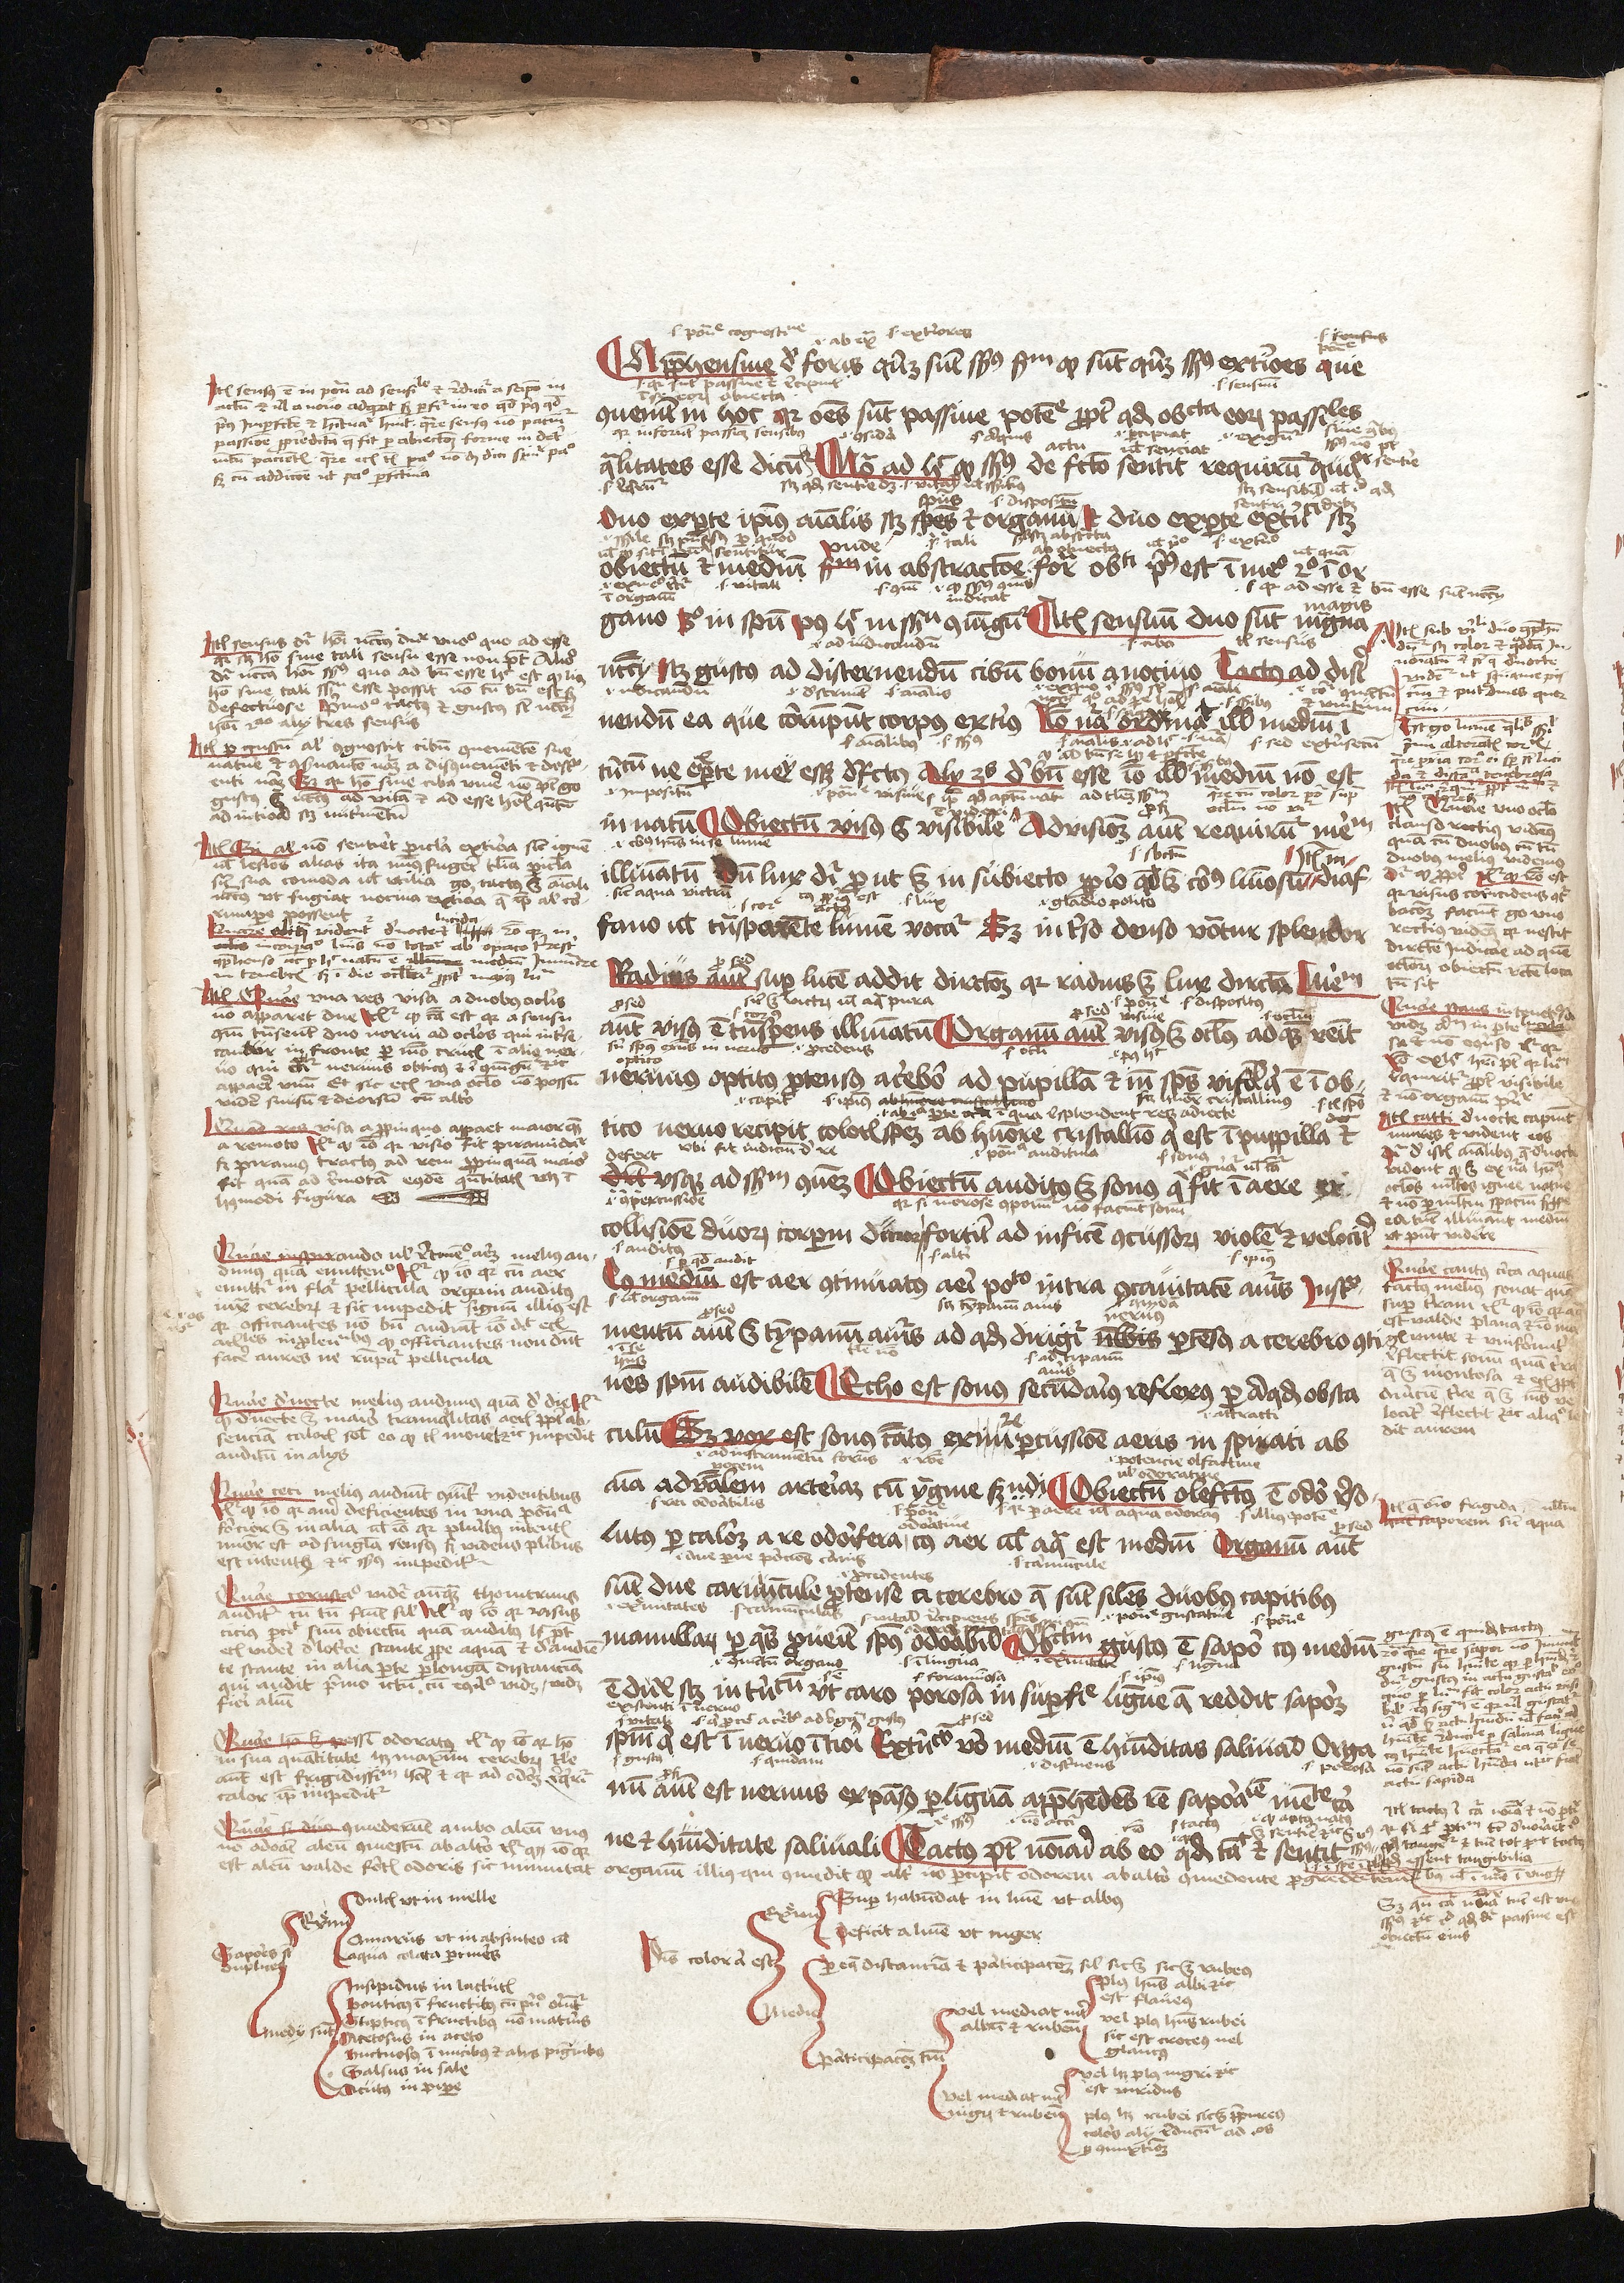
\includegraphics[width=.85\textwidth]{aristoteles_de_anima}}
\medskip

\centering{Eine Passage aus Aristoteles' De Anima in einer mittelalterlichen Handschrift mit 
Interlinear- und Marginalglossen}
}

%\subject{edition dante}

\title{\LaTeX{} für Geisteswissenschaftler}
\subtitle{Ein Überblick über die wichtigsten Hilfsmittel für die Arbeit mit 
Texten als Forschungsgegenstand}

\author{Lukas C. Bossert \and Axel Kielhorn \and Thomas Hilarius Meyer \and Craig Parker-Feldmann \and Philipp Pilhofer \and Martin Sievers \and Uwe Ziegenhagen}
\date{}
\publishers{DANTE~e.\,V.}

\lowertitleback{\copyright{} 2016 bei den Autoren
	Satz mit \LaTeXe{} und \KOMAScript (vgl. Kolophon)\\
        Haftungsausschluss: }

\maketitle

% !TeX root = lfgw.tex
\chapter{Vorwort}

Philologie bedeutet

also müssten Philologen besondere Sorgfalt und liebe zur Erstellung ...

Dieses Skript richtet sich an zwei Zielgruppen, deren Bedürfnisse verwandt, aber doch verschieden sind:

\begin{itemize}
 \item Angehörige der Geistes- und Sozialwissenschaften, die \LaTeX{} im Rahmen ihrer Arbeit
 -- sei es zur Erstellung einer Seminararbeit, einer Bachelor- oder Masterarbeit, eines
 Dissertationsprojektes oder eines komplexen Editionsvorhabens --
 einsetzen möchten und keine oder nur sehr geringe Kenntnisse des \LaTeX{}-Systems haben.
 \item Erfahrene \TeX-niker
\end{itemize}

Am Beginn dieses Buches muss ich den Leser um Vergebung für eine eigentlich unverzeihliche begriffliche
Unsauberkeit bitten: nichtmathematische Geisteswissenschaftler!

\LaTeX{} wird von einer sehr aktiven Community weiterentwickelt.

DTK verzeichnet ca. 50 NEUE Pakete im Quartal.

Deshalb große Unübersichtlichkeit: Neulinge finden oft auch veraltetes bzw,. sehen vor lauter
Wald die Bäume nicht.

Deshalb Idee dieses Buches: Für die häufigsten Bedürfnisse im geisteswissenschaftlichen
Bereich gangbare, aktuelle Lösungen vorstellen.

Nähere Infos zur Intensiveren Nutzung enthalten immer die Paketdokumentationen.

Herzlichen Dank 
\endinput
\tableofcontents
% !TEX root = lfgw.tex
\chapter{Grundsätzliches}

Der Einsteiger in die Welt von \TeX{} und \LaTeX{} wird mit einer Vielzahl von Programmnamen und 
Spezialbegriffen konfrontiert, die zunächst einmal Verwirrung stiftet.
Wie so oft hilft ein Blick in die Geschichte, die Vielfalt der Gegenwart zu verstehen~\dots


\section{Zur Geschichte von \TeX{}, \LaTeX{} und Co. -- zugleich eine Begriffsklärung}

Am Anfang der gesamten Entwicklung steht Donald Knuth, ein US-amerikanischer Mathematiker und 
Informatiker, der mit der typografischen Qualität zeitgenössischer mathematischer Texte 
unzufrieden war:

\begin{foreigndisplayquote}{english}
 Mathematics books and journals do not look as beautiful as they used to.
 It is not that mathemathical content is unsatisfactory, rather than the old and 
 well-developed traditions of typesetting have become too expensive.
 Fortunately it now appears that mathematics itself can be used to solve this problem.%
 \footcite[Zitiert nach:][1]{voss:einfuehrung}
\end{foreigndisplayquote}

Die Antwort von Donald Knuth auf das von ihm wahrgenommene ästhetische Defizit war das  
Programm \TeX. Als Ergänzung entwickelte er das \METAFONT-System zur Definition von 
Zeichensätzen.
\TeX{} bildet bis heute, die Grundlage des Gesamtsystems, doch wurde das Programm immer 
wieder erweitert und angepasst.

Die wichtigste Erweiterung erfolgte durch Leslie Lamport der eine ganze Reihe von 
inhaltlich ausgerichteten Befehlen auf \TeX-Basis definierte: \LaTeX{} war geboren.
Die bislang letzte Version dieses Programmes -- \LaTeXe{} -- stammt aus dem Jahre 1994
und definiert das Grundgerüst. Aus Kompatibilitätsgründen gab es für diese Version nur
Fehlerkorrekturen.

Zwei Dinge haben sich seither weiterentwickelt:

Das Ausgabeformat PDF hat sich als universelles Dokumentformat durchgesetzt; es wird von neueren
\LaTeX-Entwicklungen direkt erzeugt. (\TeX{} und das ursprüngliche \LaTeX{} erzeugten DeVice 
Independent~(DVI)-Dateien, die man mit einem speziellen Druckertreiber ausdrucken,
oder zu PS- oder PDF-Dateien konvertieren konnte.)
Das ausführende Programm hieß nun \pdfLaTeX. 
Selbstverständlich versteht es auch Dateien in reinem \TeX{};
es kann per Kommandozeilenoption dazu gebracht werden, DVI-Dateien zu erzeugen, wenn dies aus 
bestimmten Gründen gewünscht ist.
Ruft man den Kommandozeilenbefehl \lstinline/latex/ auf, wird in aller Regel das Programm 
\pdfLaTeX{} gestartet.

Die zweite große Änderung betrifft das Eingabeformat:
\TeX{} und \LaTeX{} wurden so umgebaut, dass sie unmittelbar Unicode-Zeichen verstehen.
Das ist vor allem für Sprachwissenschaftler interessant, stehen doch jetzt praktisch alle Schriftzeichen
der Welt unmittelbar zur Verfügung. 
Man kann das traditionelle \pdfLaTeX-Programm mit Hilfe eines sogenannten Paketes dazu bringen, Unicode-Zeichen
zu verstehen
(Die entsprechenden Befehle heißen: \lstinline/\usepackage[utf8]{inputenc}/ 
und \lstinline/\usepackage[T1]{fontenc}/.)
oder eine speziell für die Unicode-Untersützung entwickelte \TeX{}-Version wie \XeLaTeX{} 
oder \LuaLaTeX{} verwenden.

Die neueste Entwicklung in der Welt der \TeX-Programme ist die Integration der Skriptsprache
Lua in die \TeX-engine: \LuaLaTeX{} wird als der kommende Standard gehandelt.

Dieses Buch wurde mit \LuaLaTeX{} erstellt, die meisten Beispiele funktionieren aber auch mit \pdfLaTeX{}.
Der Vorteil von \pdfLaTeX{} ist die höhere Bearbeitungsgeschwindigkeit, bei über 200 Seiten merkt man
den Unterschied.

Wenn \LuaLaTeX{} erforderlich ist, wird im Beispiel darauf hingewiesen.

\section{Arbeitswerkzeuge}

Empfehlenswert für die tägliche Arbeit mit \LaTeX{} gerade bei größeren Projekten ist eine 
IDE (Integrated Developement Environment = Integrierte Entwicklungsumgebung).
Doch zuerst sollte man die Einzelwerkzeuge kennen, die in solchen \enquote{Meta-Werkzeugen}
zusammengefasst sind.

\minisec{Einzelwerkzeuge}

\LaTeX{}-Dokumente lassen sich mit jedem beliebigen \textbf{Editor} erstellen.

Diese Buch entstand als Kooperation mehrerer Autoren, die unterschiedliche Editoren
auf unterschiedlichen Betriebssystemen benutzt haben:

\begin{itemize}
\item \Program{TeXShop} auf macOS
\item \Program{Vim} auf macOS
\item \Program{Kile} auf Linux
\item \Program{\TeX{}studio} auf Debian GNU/Linux
\end{itemize}

\marginnote{Bitte ergänzen}

Das ist möglich, da es sich bei den Dateien um reine Textdateien handelt.

Doch es gibt ein paar Qualitätsmerkmale, auf die man bei der Auswahl achten sollte, weil
sie die tägliche Arbeit wesentlich erleichtern:

\begin{labeling}{\Program{TechnicCenter}}

\item[Syntaxhervorhebung] (Highlighting) hebt \LaTeX-Befehle sowie bestimmte
  Inhalte wie Überschriften etc. farblich hervor, was die Übersicht über das
  Dokument wesentlich erleichtert. Auch die Navigation in den manchmal
  geschachtelten geschweiften Klammern kann durch einen guten Editor
  wesentlich erleichtert werden: Fährt man eine schließende Klammer an, wird
  die jeweils dazugehörende öffnende Klammer hervorgehoben.

\item [Unicode Unterstützung] sollte im 21.\ Jahrhundert selbstverständlich
  sein.  Zur Darstellung benötigt man einen geeigneten Zeichensatz, der die
  erforderlichen Symbole enthält. Alle hier vorgestellten Programme
  unterstützten Unicode.

\item [Faltung] Einige Editoren erlauben es Umgebungen oder Abschnitte
  einzufalten.  Es bleibt dann nur noch die erste Zeile sichtbar. So behält
  man auch bei großen Dokumenten den Überblick.

\item [Synchronisation] (SyncTeX) zwischen Eingabe und PDF ermöglicht es im
  Quelltext auf eine Textstelle zu klicken und in der entsprechenden Stelle
  im PDF zu landen, bzw.  umgekehrt aus dem PDF in den Quelltext
  zurückzuspringen. Hier sind die IDEs den Editoren klar überlegen.

\end{labeling}

Bei der Auswahl des Programms für die Bearbeitung kann man grundsätzlich zwischen Texteditoren und kompletten Entwicklungsumgebungen unterscheiden.
Die Texteditoren einigen sich dafür, kleinere Korrekturen vorzunehmen.
Für die umfassendere Bearbeitung eignen sich komplette Entwicklungsumgebungen.
Auch hier ist es Geschmackssache des Urhebers, welches Werkzeug er bevorzugt.
Im Folgenden sollen Repräsentanten für beide Kategorien vorgestellt werden.

Einige empfehlenswerte Editoren mit grundlegender Unterstützung für die Arbeit mit \LaTeX{} sind die folgenden:

\begin{labeling}{\Program{TechnicCenter}}
\item[\Program{kwrite}] (Linux) 

\item[\Program{kate}] (Linux)

\item[\Program{Notepad++}] (Windows) \url{https://notepad-plus-plus.org} Ein
  kostenloser Editor mit Syntaxhervorhebung.  

\item[\Program{TextEdit}]
  (macOS) Dieser Editor wird mit dem Betriebssystem ausgeliefert.  Anders
  als der Name vermuten lässt, speichert er jedoch keinen reinen Text
  sondern RTF.  Eine Datei muss vor dem Speichern in reinen Text umgewandelt
  werden.

\item[\Program{Atom}] (Windows + Linux + macOS)
  \url{https://atom.io} Der Editor von GitHub.  Es gibt Erweiterungspakete
  die Syntaxhervorhebung sowie den Aufruf von \LaTeX{} nachrüsten.

\item[\Program{Vim}] (Windows + Linux + macOS) \url{http://www.vim.org} Eine
  verbesserte Version des Klassikers \Program{vi}. \Program{Vim} bietet
  neben der Syntaxhervorhebung eine Funktion zum Falten des Textes. Öffnet
  man eine Datei, so sind nur die Überschriften sichtbar. Das erleichtert
  besonders bei großen Dokumenten die Navigation.  Die
  \Program{vim-latex-suite} erweitert den Editor zu einer IDE, die meisten
  Befehle können dann mit zwei bis drei Tasten eingegeben werden, außerdem
  werden die geschweiften Klammern automatisch eingefügt, gerade auf einer
  deutschen Tastatur ist das extrem hilfreich.  Zusätzlich bietet er mit
  \Program{fugitive} eine Integration in die Versionsverwaltung
  \Program{git}.  \Program{Vim} ist ein sehr mächtiges Werkzeug, das den
  Anfänger leicht überfordert.  Für den langjährigen \Program{VIM}-Nutzer
  ist es jedoch unverständlich, wie jemand etwas anderes benutzen kann.
  \Program{Vim} ist Charityware, der Autor bittet um Spenden für Waisenkinder in Uganda.

\item[\Program{Emacs}] (Windows + Linux + macOS) 
  \url{https://www.gnu.org/software/emacs/emacs.html} In Verbindung mit
  \Program{AucTeX} ist der Emacs eine integrierte Entwicklungsumgebung
  für alle, die nicht ständig zur Maus greifen wollen.  Der Einstieg ist
  noch etwas schwieriger als beim \Program{Vim}, dafür dafür gibt es auch
  deutlich mehr Funktionen. Selbstverständlich ist auch hier eine
  Versionsverwaltung integriert.  Für Anfänger ist der \Program{Emacs} nur
  dann geeignet, wenn am Nachbartisch ein erfahrener Emacs-Anwender sitzt.
  Selbst dann verbringt man leicht mehr Zeit damit \Program{Emacs} zu
  lernen, als damit \LaTeX{} zu lernen. Für den langjährigen 
  \Program{Emacs}-Nutzer ist es jedoch unverständlich, 
  wie jemand etwas anderes benutzen kann.
  
  Der \Program{Emacs} wird von der Free Software Foundation entwickelt
  und ist frei (wie in Freiheit) verfügbar.
\end{labeling}

\minisec{Kommandozeile}

Eine \LaTeX{}-Standardinstallation enthält über 400 Programme, von denen man zu Glück nur einen Bruchteil benötigt.

\begin{labeling}{makeindex}
\item[\Program{pdflatex}] Ein \LaTeX{} das weitgehend dem Stand von 1982 entspricht, jedoch direkt PDF-Dateien erzeugen kann.
\item[\Program{xelatex}] Ein \LaTeX{} mit Unicode Unterstützung und der Möglichkeit von rechts nach links zu schreiben.
\item[\Program{lualatex}] Ein \LaTeX{} mit Unicode Unterstützung und integrierter Programmiersprache.
\item[\Program{biber}] Das Programm zum Erstellen des Literaturverzeichnisses.
\item[\Program{makeindex}] Ein Programm zum Erstellen eines Schlagwortverzeichnisses.
\end{labeling}

\minisec{Integrierte Entwicklungsumgebungen (IDE)}

\begin{labeling}{\Program{TechnicCenter}}
\item[\Program{TeXShell}] (Atari ca. 1990) Der Atari war wegen seiner
  grafischen Oberfläche sehr beliebt.  Natürlich wollte niemand auf so
  einem Rechner eine Kommandozeile benutzen.  Zum Glück gab es mit der
  \Program{TeXShell} eine Oberfläche, die die einzelnen Programme hinter
  Knöpfen versteckte.  Eine farbliche Syntaxhervorhebung gab es natürlich
  nicht, das hätte auf dem Monochrommonitor auch nichts gebracht.

\item[\Program{TexnicCenter}] (Windows 1999)
  \url{http://www.texniccenter.org}  Bei Windows-Nutzern ist die
  Kommandozeile noch weniger beliebt als bei Atari-Nutzern.  Das
  \Program{TexnicCenter} war die erste wirklich integrierte
  Entwicklungsumgebung.  So konnte man \LaTeX{} ohne \Program{command.com}
  benutzen.

\item[\Program{Texshop}] (macOS 2001)
  \url{http://pages.uoregon.edu/koch/texshop/about.html}  Kurz nach dem
  Erscheinen von macOS (née OS X) erschien mit \Program{TeXShop} eine IDE
  für den Mac.  Nach heutigem Standard ist der Funktionsumfang eher
  minimalistisch, aber Syntaxhervorhebung und Makros zum Aufrufen der
  gängigen \LaTeX{}-Befehle sind vorhanden.  Durch den geringen
  Funktionsumfang ist das Programm sehr aufgeräumt.

\item[\Program{TeXworks}] (Win + Linux + macOS 2009)
  \url{https://www.tug.org/texworks/}  Da \Program{TeXShop} nur auf dem Mac
  läuft, wurde versucht mit \Program{TeXworks} eine Version für alle
  gängigen Betriebssysteme zu schaffen.  Das Design ist eher aufgeräumt und
  übersichtlich.

\item[\Program{TeXStudio}] (Win + Linux + macOS 2009)
  \url{https://www.texstudio.org/}  Das rundum sorglos Programm für
  große Projekte.
  Neben den üblichen Features der Syntaxhervorherbung enthält es insbesondere folgende zwei Features enthält:
  Unterstützung der Grammatikprüfung mittels LanguageTool (\url{https://languagetool.org/de/}) und der Sprung vom PDF zum \LaTeX{}-Quelltext.
  Weiterhin bietet \Program{TeXStudio} neben einem Projektbrowser, der alle zum Projekt
  gehörenden Dateien zeigt, bietet auch eine integrierte
  Versionsverwaltung mit \Program{SVN}.  Die Syntaxhervorhebung erkennt die
  verwendeten Pakete und lädt die benötigten Definitionen bei Bedarf nach.
  So werden ungültige Befehle erkannt und farblich markiert, man merkt den
  Tippfehler also schon bei der Eingabe. Außerdem lassen sich Umgebungen
  und Abschnitte einfalten.

\item[Kile] (Win + Linux) \url{http://kile.sourceforge.net}

\end{labeling}

\minisec{Online-Lösungen}

Mit Overleaf\footcite{meyer:dtk2015/1} \url{https://www.overleaf.com}\index{overleaf}
gibt es eine Möglichkeit \LaTeX-Dokumente im Internet zu bearbeiten.
So spart man sich die Installation und kann von jedem Rechner darauf zugreifen.
Allerdings sind die Daten dann auch im Internet und man muss sich auf den Datenschutz der Betreiber verlassen.

Die Minimalversion ist kostenlos, ein erweitertes Paket für bis zu 10 Mitarbeiter pro Projekt kostet 14~Euro im Monat.
(Stand 2019)

Das Projekt Sharelatex\index{sharelatex} \url{www.sharelatex.com}  wurde von Overleaf übernommen und existiert
nicht mehr als eigenes Angebot.

\section{Erste Schritte in \LaTeX}

Anlegen einer Datei

Dokumentstruktur: Präambel, Dokumentklasse etc.

Übersetzen der \LaTeX{}-Datei

Betrachten und evtl. Ausdrucken der PDF-Datei


\section{Musterprojekt: eine beispielhafte Hausarbeit}

Angenommen, wir sollen eine Hausarbeit schreiben.
Wir wollen Grafiken einbauen, unsere Literatur automatisch verarbeiten und ein Register erstellen.
Außerdem soll die Typografie schön sein.

Also brauchen wir für den Anfang erst einmal eine Datei mit ein paar Zauberworten:


\minisec{Datei: hausarbeit.tex}

\begin{lfgwcode}{label={hausarbeit}}
% !TEX TS-program = pdfLaTeX
% !TEX encoding = UTF-8
\documentclass[german]{scrreprt}
 
\usepackage[utf8]{inputenc}
\usepackage[T1]{fontenc}

\usepackage[ngerman]{babel}
\usepackage{csquotes}

\usepackage{graphicx}

\usepackage{imakeidx}

\usepackage[style=verbose-inote,pageref=true]{biblatex}
\addbibresource{meine-bibliographie.bib}

\title{\LaTeX{} und der Sinn des Lebens}
\subtitle{Eine vielosofische Hausarbeit}

\author{Eberhard Knesenbeck}
\date{[Stand: \today]}

\begin{document}

\maketitle

\tableofcontents

blubb, blah \dots

\printbibliography
\end{document}
\end{lfgwcode}

Was bedeuten die Anweisungen im einzelnen?

\begin{labeling}{3-4}

 \item[1-2] Zeilen, die mit einen \%-Zeichen beginnen, sind Kommentare und
   werden von \LaTeX{} ignoriert. Bei diesen beiden Zeilen handelt es sich
   um Anweisungen an die IDE, die so die richtige Codierung und das
   erforderliche Programm erfährt.  Leider sind sich die unterschiedlichen
   IDEs nicht einig, welche Parameter wie codiert werden, mal sind die
   Leerzeichen um das Gleichheitszeichen erforderlich, mal sind sie
   verboten.

 \item[3] Das Einstellen der Dokumentklasse definiert das grundsätzliche
   Aussehen des Textes: geht es um ein Buch, einen Artikel oder -- wie hier
   -- eine Hausarbeit.  Die Angabe \lstinline/scrreprt/ bedeutet, dass ein
   \enquote{Report} (also z.\,B. eine Hausarbeit) mit Hilfe der Definitionen
   des \KOMAScript-Paketes von Markus Kohm erstellt werden soll.  (Mehr dazu
   vgl. S.~\pageref{komaskript}) Das Buch (\lstinline/book//\lstinline/scrbook/)
   oder der Report  (\lstinline/report//\lstinline/scrreprt/) haben
   als oberste Gliederungsebene das Kapitel (\lstinline/\chapter/), der Artikel
   (\lstinline/article//\lstinline/scrartcl/) dagegen \lstinline/\section/.
   Dadurch ist es möglich mehrere Artikel zu einem Report oder Buch zusammenzufassen.
 
 \item[5-6] Zwei Zauberzeilen, die dazu führen, dass alle möglichen
   Unicode"=Sonderzeichen benutzt werden dürfen und auch ausgegeben werden
   können wie z.\,B. ä, ö, ü, ß, æ, ï oder þ.  (Achtung! Der Editor muss auf
   Unicode eingestellt sein! -- vgl. S.~\pageref{unicode} und die verwendete
   Schrift muss die Zeichen enthalten.)
 
 \item[8-9] \LaTeX{} benutzt jetzt deutsche Begriffe (Bibliographie statt
   Bibliography) und Silbentrennmuster (\paket{babel}).\footnote{Etwas
   genauer: Es gelten die Regeln der Rechtschreibreform von 1996.
   Sollen die Regeln von 1901 gelten, muss als Option stattdessen
   \lstinline/german/ angegeben werden. Vgl. \ref{babel} auf
   S.~\pageref{babel}} Außerdem werden deutsche Gepflogenheiten bei
   den Anführungszeichen verwendet (\paket{csquotes}).  Die beiden
   Zaubersprüche sollten in keiner deutschen Datei fehlen.
 
 \item[11] Das Paket \paket{graphicx} ist ein mächtiges Werkzeug um Grafiken
   einzubinden.  Wir laden es vorsorglich; wenn unser Text nicht lang genug
   ist, können wir Bilder dazunehmen \dots
 
 \item[13] Das paket \paket{imakeidx} wird uns später erlauben, sehr einfach
   ein Register zu unserer Arbeit auszugeben.  Für komplexere Aufgaben wie
   Orts- und Personenregister, Bibelstellenregister etc. lässt sich imakeidx
   umfangreich konfigurieren.
 
 \item[15-16] Diese beiden recht abschreckenden Zauberformeln werden uns
   erlauben, unsere gesamte Literaturverwaltung mit allen Formalien
   automatisch erledigen zu lassen.  Hier sagen wir \LaTeX{}, dass wir
   unsere Bibliographiedaten in einer Datei namens
   \file{meine-bibliographie.bib} aufheben, dass das Programm
   \Program{biblatex} für uns die Arbeit machen soll und dass es sich dabei
   an einem bestimmten, eher traditionellen geisteswissenschaftlichen Stil
   ausrichten soll.

 \item[18-19] Erst mal legen wir einen guten Titel und Untertitel fest \dots

 \item[21] \dots\ und sagen, wer wir sind.
 
 \item[22] Diese Zeile sorgt dafür, dass auf dem Titelblatt das jeweils
   aktuelle Datum als Stand der Arbeit ausgegeben wird. Das kann praktisch
   sein, wenn man seltener seinen Schreibtisch aufräumt, als neue Fassungen
   ausdruckt.\\ Achtung! Soll (z.\,B. in der Endfassung) kein Datum
   ausgegeben werden, so muss man explizit \lstinline/\date{}/ angeben.
   Löscht man die \lstinline/\date/-Anweisung ganz, wird automatisch das
   heutige Datum ausgegeben!

 \item[24] Jetzt wird es ernst: Unser eigentliches Dokument beginnt.
 
 \item[26] Achtung! Erst mit dem Befehl \lstinline/\maketitle/ wird \LaTeX{}
   dazu gebracht, die definierten Titelseiten auch wirklich
   \emph{auszugeben}!

 \item[28] Dieser Befehl gibt das Inhaltsverzeichnis aus.

 \item[30] Jetzt kommen endlich unsere wertvollen Inhalte.
 
 \item[32] Hier wird das automatisch erstellte Literaturverzeichnis ausgegeben.
 
 \item[33] Diese letzte Zeile schließt das \LaTeX{}-Dokumente ab.

 \end{labeling}

Das gleiche Beispiel nun mit \LuaLaTeX{}, es ändern sich nur drei Zeilen.
 
\begin{lfgwcode}{label={hausarbeit-lualatex}}
% !TEX TS-program = LuaLaTeX
% !TEX encoding = UTF-8
\documentclass[german]{scrreprt}
 
\usepackage{fontspec}

\usepackage[ngerman]{babel}

\begin{document}

\end{document}
\end{lfgwcode}

\begin{labeling}{3-4}

 \item[1] Hier wird jetzt \LuaLaTeX{} als zuständiges Programm ausgewählt. 
  
 \item[5] \Paket{inputenc} und \Paket{fontenc} werden nicht mehr benötigt,
   stattdessen übernimmt \Paket{fontspec} das Laden der Zeichensätze.  Die
   Standardschrift ist jetzt \texttt{Latin Modern Roman}, die Unterschiede
   zu \texttt{Computer Modern Roman} sind aber nur minimal. 

 \item[7] Babel funktioniert auch mit \LuaLaTeX{}.
 
 \item[9] Jetzt wird es ernst: Unser eigentliches Dokument beginnt.
 
 \item[11] Diese letzte Zeile schließt das \LaTeX -Dokumente ab.

 \end{labeling}

 
\minisec{Datei: meine-bibliographie.bib}

Damit sich die Datei kompilieren lässt, muss die in Zeile 16 angekündigte Datei mit 
bibliografischen Angaben auch existieren!

Sie habe einen einzigen Eintrag mit einem wichtigen Buch für \LaTeX -Einsteiger.
Legen wir sie an:

\begin{lfgwcode}{label={hausarbeit-bib}}
@Book{voss:einfuehrung,
 author    = {Herbert Voß}, 
 title     = {Einführung in \LaTeX},
 publisher = {DANTE~e.\,V. and Lehmanns Media},
 location  = {Berlin and Heidelberg},
 year      = {2016},
 edition   = {2},
}
\end{lfgwcode}

Die Bibliografie-Datei unseres Projektes enthält also einen einzigen Eintrag:
\bigskip

\framebox[75mm]{
  \parbox{65mm}{
    \cite{voss:einfuehrung}
  }
}
\parbox{40mm}{
   \emph{übrigens sehr lesenswert \dots}
}
\bigskip

Dieser Titel ist übrigens automatisch aufgelöst worden; 
in der Datei steht nur \lstinline/\cite{voss:einfuehrung}/.
Allein diese Funktionalität -- und all die Tricks, die sich in dem Zusammenhang anstellen
lassen, rechtfertigen den Einsatz von \LaTeX{} und Co. (Mehr dazu S.~\pageref{biblatex}\,ff.)

\section{Allgemeine Literatur}

Dieses Buch behandelt die besondren Anforderungen der Geisteswissenschaften.
Es ist ausdrücklich \emph{keine} Einführung in \LaTeX.
Das ist auch nicht notwendig, da es zu diesem Thema bereits genug Literatur gibt.

Das erste Dokument, die \citetitle{l2kurz} \parencite{l2kurz}, wird normalerweise mit \TeX{} mitgeliefert.
Mit dem Befehl \lstinline/texdoc l2kurz/ in der Kommandozeile wird es automatisch aufgerufen.
Ansonsten kann man im \TeX\ Verzeichnis nach \lstinline/l2kurz.pdf/ suchen.
Dieses Dokument erklärt auf weniger als 60 Seiten die Grundlagen um mit \LaTeX{} zu arbeiten.

Mit knapp 1000 Seiten ist die \citetitle{voss:einfuehrung} \parencite{voss:einfuehrung} deutlich ausführlicher
und bietet weit mehr als eine Einführung.

\citetitle{kohm:2020} \parencite{kohm:2020} vom Markus Kohm beschreibt die vom ihm entwickelten Dokumentklassen.
Es ist somit ein sehr spezielles Buch, da es sich nur mit einem Packet beschäftigt.
Die in diesem Paket definierten Klassen haben im europäischen Raum eine große Bedeutung 
und dienen anderen Klassen (z.\,B. Dissertationen verschiedener Universitäten) als Basis.
Sie sind ein guter Ausgangspunkt für eigene Dokumente, da sie bereits viele Layoutdetails gut umsetzen.
Außerdem gibt es Optionen um das Layout an die eigenen Wünsche anzupassen.
Eine gekürzte Version des Buches wird mit \TeX{} mitgeliefert und kann mit \lstinline/texdoc scrguide/ aufgerufen werden.

Für dieses Buch wird die Klasse \lstinline/scrbook/ aus dem KOMA-Sript Paket verwendet.

Neben klassischen Büchern gibt es auch einige Online Quellen.
Hier ist besonders \url{https://www.learnlatex.org/de/} zu empfehlen.
Theoretisch soll es hier auch eine deutsche Anleitung geben, 
für die meisten Artikel existiert aber nur das englische Original.

Das Forum \url{https://golatex.de} bietet die Möglichkeit Fragen zu stellen, 
diese werden dann von anderen Nutzern beantwortet.
Natürlich empfiehlt es sich vorher nach ähnlichen Fragen zu suchen.

\endinput



% !TeX root = lfgw.tex
%\chapter{Typographische Gestaltung}
% !TEX root = lfgw.tex

\chapter{Texte schreiben}
\autor{Thomas Hilarius Meyer}

Geistes- und humanwissenschaftliche Arbeiten haben besondere Anforderungen an die typografische
Gestaltung.
Die häufigsten Anforderungen werden im folgenden der Reihe nach durchgegangen.
Manches davon ist \LaTeX-Standard; anderes wird außerhalb der Geisteswissenschaften eher
selten gebraucht.
Ein großer Bereich, für den \LaTeX{} eigentlich bekannt ist, bleibt ganz außen vor:
der Satz von komplexen mathematischen Formeln und Gleichungen.


\section{Vorüberlegungen zu typografischer Schönheit und Funktionalität}

\dictum[Louis Sullivan]{Form follows function.}

Der Grundgedanke bei der Benutzung von \LaTeX\ ist, dass sich der Autor um die inhaltliche Seite seines
Textes kümmert, und die typografische Aufbereitung den Algorithmen der Software überlässt,
die aus der ihr mitgeteilten logischen Struktur anhand der traditionellen Regeln funktionaler Setzerkunst
eine schön -- im Sinne funktionaler Ästhetik -- aufbereitete Druckfassung erstellt.

Dieser Ansatz widerspricht der weitverbreiteten Do-it-yourself-Mentalität der Typografie des
PC-Zeitalters, die im sehr lesenswerten Leitfaden \enquote{Erste Hilfe Typografie} der Setzer-Koryphäen
Hans Peter Willberg und Friedrich Forssmann karikiert wird:

\begin{quote}
 Das Selbermachen ist längst üblich, die Ergebnisse sind oft fragwürdig,
 weil die Laien-Typografen nicht sehen, was nicht stimmt und nicht wissen
 können, worauf es ankommt.
 So gewöhnt man sich an falsche und schlechte Typografie.
 \footcite[9]{erste_hilfe}
 \end{quote}

\begin{quotation}
 \emph{Du warst doch mal Sekretärin.
 Ich muss meine Diss schreiben, kannst Du mir zeigen, wie das geht?}

 \emph{Was} ein Doktorand oder Diplomand zu schreiben hat, das hat er studiert.
 \emph{Wie} er es zu schreiben hat, hat er nicht studiert, er setzt irgendwie drauflos.
 Mit unübersichtlicher und schlecht lesbarer Laien-Typografie schadet er oft genug seiner Arbeit.
 \footcite[86]{erste_hilfe}
\end{quotation}

Natürlich beinhaltet auch eine moderne \LaTeX -Installation keine künstliche Intelligenz mit
vollständiger Setzerlehre und vor allem sind die Spezialanforderungen gerade an die Satzerstellung im
humanwissenschaftlichen Bereich so speziell und individuell, dass es gelegentlich nicht ohne
\enquote{Selbermachen} und \enquote{Basteln} geht, aber dennoch ist es wichtig, sich den Grundsatz
klarzumachen: In einem \LaTeX -Dokument wird primär der \emph{Inhalt} ausgezeichnet, und erst sekundär
die Repräsentation der inhaltlichen Struktur in ein Druckbild.

Um was geht es im einzelnen beim Erstellen von Texten mit \LaTeX ?


\section{Wahl der Dokumentklasse}

In der ersten Zeile eines \LaTeX -Dokumentes wird die Dokumentklasse des folgenden Textes
festgelegt. Die Dokumentklasse definiert die grundsätzlichen Spielregeln:
Welche Gliederungsebenen sind vorgesehen, wie ist die grundsätzliche Formatierung aufgebaut etc.

Es existiert eine sehr große Vielzahl von verschiedenen Dokumentklassen;
so gibt es für Hausarbeiten oder Dissertationen zahlreicher Universitäten eine eigene
Dokumentklasse. Existiert eine solche, sollte man sie i.\,d.\,R. auch benutzen.

Die folgende Einführung beschränkt sich auf die Klassen des \KOMAScript-Paketes von
Markus Kohm, weil diese eine überragende typografische Qualität sowie zahllose Möglichkeiten
zur individuellen Anpassung bieten.%
\footnote{Wer allerdings ihre volle Funktionalität nutzen will, sollte sich die originale
Dokumentation beschaffen und sich mit ihrer Hilfe genauer einarbeiten \dots}
Hinzu treten zwei Dokumentklassen für speziellere Fälle, nämlich für Präsentationen und
Prüfungen.

\begin{labeling}{scrreprt}
 \item[scrartcl] ist die \KOMAScript-Klasse für Artikel.
 \item[scrreprt] kann gut für längere Seminar- oder auch Bachelor-Arbeiten genutzt werden.
 \item[scrbook] ist die Klasse für Bücher mit zahlreichen ausgereiften Funktionen für
  die Titelei etc.
 \item[exam] ist eine eigene Klasse zur Entwicklung von Aufgabenblättern zu Prüfungszwecken.
 \item[beamer] stellt eine ganze Reihe von Features für die Erstellung von Präsentationen
  zur Verfügung. Mit etwas Einarbeitung gelingen damit schneller bessere Präsentationen als
  mit der verbreiteten Konkurrenz.
\end{labeling}


\minisec{Zum Unterschied zwischen \enquote{Klasse} und \enquote{Paket}}

\dictum[Goethe, Faust 1337]{Was ist mit diesem Rätselwort gemeint?}

In \LaTeX -Kreisen ebenso wie innerhalb dieser Anleitung ist häufig von \enquote{Paketen} die Rede,
die \enquote{geladen} werden müssen, um eine bestimmte Funktionalität zu gewährleisten.
Andererseits stellen zahlreiche \enquote{Klassen} bereits Features zur Verfügung etc.
-- wie sind diese Begriffe zu verstehen?

Eine \textbf{Dokumentklasse} definiert die grundlegende Struktur zur Bearbeitung einer Textgattung
mit Hilfe von \LaTeX. Das kann ganz allgemein sein -- wie die ursprünglichen Standardklassen book, report,
article -- oder sehr speziell -- wie die Vorlage einer Dissertation in Elektrotechnik an einer ganz
bestimmten Technischen Hochschule.

Die gewünschte Dokumentklasse wird ganz am Anfang angegeben durch das Kommando
\cs{documentclass\oarg{Optionen}\marg{NAME}}.
% sollte hier nicht deutlich gemacht werden, dass LaTeX genau dies
% auszeichnet: man muss nicht mit den atomaren Elementen aus TeX arbeiten,
% sondern nutzt eine Dokumentenklasse, die viele Detaileinstellungen vornimmt
% und darüber hinaus eine Reihe von logisch strukturierenden Voreinstellungen
% bereitstellt, die für den jeweiligen Anwendungsfall festgelegt wurden.
% Auch könnte auf die Äquivalenz zwischen Dokumentenklasse und Vorlagen bei
% Textverarbeitungssystemen hingewiesen werden.

Grundsätzlich gilt: Je spezieller eine Dokumentklasse ist, desto genauer passt sie zu einer spezifischen
Aufgabenstellung und desto eher wird sie spezifische Sonderanforderungen befriedigen -- bis hin zur
Integration des Universitätslogos etc.
Je allgemeiner eine Klasse ist, desto eher wird man bei Spezialbedürfnissen darauf angewiesen sein,
diese auf anderem Wege zu implementieren.
Jetzt kommen die Pakete ins Spiel:

\textbf{Pakete} erweitern die Funktionalität einer %beliebigen
Dokumentklasse um einzelne, meist
thematisch zusammenhängende Funktionen. Beispiele sind etwa die Möglichkeit zur Einbindung von
Grafiken, die Erstellung von Registern, bessere Möglichkeiten zur Erstellung von komplexen Tabellen etc.
Die meisten in dieser Anleitung vorgestellten Möglichkeiten basieren auf besonderen Paketen, die
oftmals von und für Geisteswissenschaftler[n] entwickelt wurden.

Das \enquote{Laden} eines Paketes erfolgt durch den Befehl \cs{usepackage}\oarg{Optionen} \marg{PAKETNAME}

Dokumentklassen und Pakete enthalten in der Regel eine ziemlich gute Dokumentation, die man
ggf. zu Rate ziehen sollte, um ihren vollen Funktionsumfang ausnutzen zu können.%
\footnote{Wie kann man die Paketdokumentation aufrufen?
    Vgl. hierzu \ref{paketdoku} auf S.~\pageref{paketdoku} }


\section{Nationale Besonderheiten -- das Paket babel}
\label{babel}

\dictum[Gen 11,7]{Wohlan, lasst uns hinabfahren und daselbst ihre Sprache verwirren, dass keiner mehr
    des anderen Sprache verstehe.}

Das vielleicht wichtigste Paket, das in praktisch jedem Dokument zu laden ist, heißt \paket{babel}.
Es sorgt dafür, dass \LaTeX\ an die verschiedenen nationalsprachlichen Besonderheiten angepasst wird.
Das betrifft auch automatisch eingesetzte Begriffe wie \enquote{Kapitel} statt \enquote{chapter} sowie
sprachspezifische typografische Regelungen.

Der Aufruf des Paketes \paket{babel} erfolgt wie bei allen Paketen:
% Ich würde nicht von Aufruf, sondern von Bereitstellen der Funktionalität sprechen
\cs{usepackage\oarg{Liste mit benutzen Sprachen}\marg{babel}}
Die in der Liste zuletzt angegebene Sprache ist die Standardsprache des Dokuments.
%(die am Anfang eingestellt ist) dar.

Babel unterstützt eine ganze Reihe von Sprachen; für Geisteswissenschaftler am wichtigsten sind
wohl:

\begin{labeling}{polutonikogreek}
 \item[german] Deutsch, alte Rechtschreibung (1901)
 \item[ngerman] Deutsch gemäß der Rechtschreibreform von 1996
 \item[greek] Neugriechisch (nur Akut, keine \emph{spiritus}, wahrscheinlich auch kein \emph{Iota subscriptum})
%von Philipp angepaßt, war vorher:
% \item[polutonikogreek] (XXX was ist der Unterschied)
 \item[greek.ancient] oder \ldots
 \item[polutonikogreek] Altgriechisch (Akut, Gravis, Zirkumflex; spiritus lenis und asper; Iota subscriptum)
\end{labeling}


Auch der Dokumentklasse sollte man die Standardsprache des Dokumentes bekanntgeben.
Denn zahlreiche Pakete, die später geladen werden, werten diese Sprachoption aus und
passen sich an (z.\,B. \paket{varioref}).
% Ausdruck ist anthropomorphisierend -- nicht passen sich an, sondern
% passen sprachsensible Konstruktionen an

Somit ergibt sich folgender typischer Dokumentbeginn:

\begin{lfgwcode}{label={lis:dokumentbeginn}}
 \documentclass[ngerman]{scrreprt}
 \usepackage[polutonikogreek,ngerman]{babel}
\end{lfgwcode}

(Wenn keine griechischen Einschübe benutzt werden, kann die Angabe von \lstinline/polutonikogreek/
%natürlich wegbleiben.)
entfallen.)

\minisec{Wechsel zu einer anderen Sprache}

Im laufenden Dokument kann auf eine der im Paketaufruf angegebenen Sprachen umgeschaltet werden:

\begin{lfgwcode}{label={lis:sprachumschaltung}}
 \selectlanguage{polutonikogreek}
\end{lfgwcode}


%\minisec{Alternative: Das Paket \paket{polyglossia}}
%
%\paket{polyglossia}


\section{Seitengestaltung und Seitenspiegel}
\label{komaskript}
\index{Seitenspiegel} \index{Goldener Schnitt}

Die folgenden Angaben sind nur von Interesse, wenn man als Papierformat nicht DIN"~A4-Papier
nutzen will und/oder nicht die eingebauten Satzspiegelkonstruktionen verwenden kann.
In den allermeisten Fällen empfiehlt es sich, den Vorgaben insbesondere der Dokumentklassen von
\KOMAScript{} zu überlassen, wie das Verhältnis von bedrucktem Bereich und Rändern aufzuteilen ist,
da der Klassenautor Markus Kohm sehr viel Aufwand in die Definition des Satzspiegels gesteckt hat und
klassische Ideale wie den Goldenen Schnitt berücksichtigt.

Dazu reicht es, bei der Angabe der Dokumentklasse das Papierformat als Option \lstinline/paper=.../ anzugeben.
Vordefiniert sind: letter, legal, executive, a0, a1, a2, a3, a4, a5, a6, a7, a8, b0 bis b8, c0 bis c8 und
d0 bis d8.
% statt
% a0, a1, a2, a3, a4, a5, a6, a7, a8
% besser: a0 bis a8
%

Außerdem ist es möglich, die Breite und Höhe des Papiers direkt anzugeben:
\lstinline/paper=200mm:200mm/.

Lediglich, wenn z.\,B. spezielle Vorgaben des Verlages es erforderlich machen, empfiehlt es sich
die Einstellungen der Seitenränder sowie ihrer zahlreichen Bestandteile (Marginalspalten, Bereiche
für Fußnoten und Seitenzahlen, Kolumnentitel usw.) direkt zu verändern.


\minisec{Direktes Einstellen des Papierformats und Satzspiegels}

Dies lässt sich am einfachsten mit Hilfe des Paketes \paket{geometry} von Hideo Umeki erreichen.
Mit seiner Hilfe ist es problemlos möglich, besondere Wünsche des Verlages hinsichtlich der Satzspiegelgestaltung zu erfüllen. Das Paket übergibt dem Nutzer die volle Kontrolle über die
Randeinstellungen -- überlässt ihm aber auch die ganze Verantwortung in ästhetischer Hinsicht.

\minisec{Beschnittmarken}
\index{Beschnittmarken}

Wenn man eine Druckvorlage für ein besonders Papierformat erzeugt, aber seine Korrekturausdrucke
auf üblichen DIN"~A4-Papier erstellt, kann man sich die \enquote{wirklichen} Größenverhältnisse von
Textblöcken und Rändern oft nicht gut vorstellen.

Hier hilft das Paket \paket{crop}, das Randmarkierungen, Beschnittmarken, in verschiedener
Ausprägung erzeugt, wie sie auch von manchen Buchbindereien gewünscht werden, um den Buchblock
präzise auf das endgültige Maß zuschneiden zu können.


\minisec{Ein- oder zweiseitiges Layout}

Bei der Einstellung der Dokumentklasse kann durch die Optionen \opt{oneside} bzw.
\opt{twoside} ein- bzw. zweiseitiges Layout verlangt werden.

Beim einseitigen Layout sind alle Seiten gleich gestaltet, während beim zweiseitigen Layout zwischen
linken und rechten Seiten unterschieden wird. Definitionsgemäß haben \enquote{linke} Seiten gerade
Seitenzahlen und \enquote{rechte} Seiten ungerade.

Die Unterscheidung hat z.\,B. auf die Positionierung der Seitenzahlen (mittig oder außen),
Kolumnentitel und Marginalien Einfluss.


\section{Textgliederung}

\minisec{Automatischer Zeilenumbruch und Absatzwechsel}

\TeX\ führt den Zeilenumbruch automatisch durch.

Die Absatzgrenze wird durch eine Leerzeile markiert.

Alternativ kann durch \lstinline/\\/ ein Zeilenwechsel erzwungen werden.%
\footnote{Ganz so einfach ist es nicht.}
% Wieso nicht?
% Entweder erklären oder löschen.

\minisec{Gliederung durch Zwischenüberschriften}

\begin{lfgwcode}{}
 \begin{document}
 \part{Ein Teil des Teils}
 \chapter{Ein Kapitel}
 \section{Ein Abschnitt}
 \subsection{Ein Unterabschnitt}
 \subsubsection{Ein kleiner Unterabschnitt}

 \chapter*{Ein Kapitel ohne Eintrag im Inhaltsverzeichnis}
 \section*{Ein Abschnitt ohne Eintrag im Inhaltsverz.}
 \subsection*{Ein Unterabs. o. E. im Iv.}
 \subsubsection*{Ein kleiner Unterabschnitt o.\,E.i.\,I.}

 \chapter[Kurzfssg. f. d. Kolumnentitel]{Ein Kapitel}
 \section[Kurzfssg. f. d. Kolumnentitel]{Ein Abschnitt}
 \subsection[Kurzfssg. f. d. Kolumnentitel]{Ein Unterabschnitt}

 \end{document}
\end{lfgwcode}

Texte lassen sich in \LaTeX{} mit Hilfe eines hierarchischen Systems von Überschriften gliedern:

\begin{labeling}{Hummel}
 \item[2-6] Texte der Kategorien
    \lstinline/book/,
    \lstinline/scrbook/,
    \lstinline/report/ und
    \lstinline/scrreprt/
 bestehen aus Teilen (\lstinline/\part{}/)
 \footnote{Ehrlich gesagt: eher selten.
 \lstinline/part/
 erzeugt einen \enquote{Zwischentitel},
 der im deutschsprachigen Raum eher unüblich ist. Ausprobieren! }
 und Kapitel (\lstinline/\chapter/);
 desweiteren lassen sich alle Texte in Abschnitte und Unterabschnitte untergliedern
 (\lstinline/\section{}/ bis \lstinline/\subsubsection{}/)
 gliedern.
 Jede Überschrift beeinflusst die Kolumnentitel (s.\,u.) und erzeugt automatisch einen Eintrag
 im Inhaltsverzeichnis.

 \item[8-11] Die \enquote{Sternvarianten} der Gliederungsbefehle erzeugen die gleiche
 Formatierung der Überschriften, hinterlassen aber keinen Eintrag im Inhaltsverzeichnis.
 Außerdem werden die Überschriften nicht nummeriert.

 \item[13-15] Die Kapitel und ggf. Abschnittsüberschriften werden auch als lebende Kolumnentitel
 verwendet. Wenn sie dafür zu lang sind, kann man in eckigen Klammern einen alternativen
 Kurztitel zur Verwendung als Kolumnentitel angeben. \index{Kolumnentitel}
\end{labeling}



\section{Schriftauszeichnungen}
\index{Auszeichnungsschriften}

\dictum[Mies van der Rohe]{Weniger ist mehr.}

Innerhalb gedruckter Texte lassen sich auf drei Weisen verschiedene Passagen typografisch voneinander
absetzen:
durch eine Veränderung des Schriftschnittes,
der Schriftgröße und
der Schriftart.

\subsection{Auszeichnung über Schriftschnitt}
\index{Schriftschnitt}
\index{kursiv}
\index{Kapitälchen}
\index{fett}
\index{Unterstreichung}

Standardmäßig erlaubt \LaTeX\ die typischen Auszeichnungen:

\begin{center}
\begin{tabular}{lll}
      Befehl                &       Beschreibung                        & typograf. Bewertung \\
      \hline
 \lstinline/\emph{}/        &   \emph{hervorgehoben} (z.\,B. kursiv in recte-Texten)        &   $+$ \\
 \lstinline/\textit{}/      &       \textsl{kursiv}                     &   $--$\\
 \lstinline/\textsl{}/      &       \textsl{schräggestellt}             &   $--$\\
 \lstinline/\textsc{}/      &       \textsc{Kapitälchen}                &   $+$ \\
 \lstinline/\textbf{}/      &       \textbf{fett}                       &   $+/-$ \\
 \lstinline/\underline{}/   &       \underline{unterstrichen}           &   $-$ \\
 \lstinline/\texttt{}/      &       \texttt{Schreibmaschinenschrift}    &   ? \\
 \lstinline/\textsuperscript{}/ &   Text\textsuperscript{hochgestellt}  &     \\
 \lstinline/\textsubscript{}/ &     Text\textsubscript{tiefgestellt}    &     \\
 \end{tabular}
\end{center}

\minisec{Unterstreichungen}

In der anspruchsvolleren Typografie gelten Unterstreichungen als verpöntes Überbleibsel
aus der Schreibmaschinenzeit. Im klassischen Bleisatz wurde nicht mit Unterstreichungen
gearbeitet.

Dennoch können Unterstreichungen in Sonderfällen sinnvoll sein.

Oftmals wünscht man sich dann sogar eine größere Auswahl an verschiedenen
Unterstreichungsarten, um etwa verschiedene Textherkünfte o.\,ä. markieren zu können.

Abhilfe schafft das Paket \paket{ulem}, das verschiedene Arten der Unterstreichung
ermöglicht:

\begin{center}
  \begin{tabular}{ll}
      Befehl &      Beschreibung \\
      \hline
      \lstinline/\uline{text}/ &    \uline{einfaches Unterstreichen} \\
      \lstinline/\uuline{text}/ &   \uuline{doppeltes Unterstreichen}\\
      \lstinline/\uwave{text}/ &    \uwave{wellenförmiges Unterstreichen}\\
      \lstinline/\sout{text}/ &     \sout{Durchstreichen} \\
      \lstinline/\xout{text}/ &     \xout{Ausschraffieren von Text} \\
  \end{tabular}
\end{center}


\minisec{Texte sperren}

Eine sehr elegant-konservative typografische Möglichkeit zur aktiven Auszeichnung ist das
\textls{Sperren}
von Textpassagen. Hierzu stellt das Paket \paket{microtype} den Befehl
\lstinline/\textls{Text}/ zur Verfügung.
% Das ist jetzt nicht Ernst gemeint.
% "A man who would letterspace lower case would steal sheep" Frederic Goudy

\subsection{Veränderung der Schriftgröße}
\index{Schriftgröße}

Die Schriftgröße lässt sich sehr leicht verändern, wobei anzumerken ist, dass
die konkrete Bedeutung der Größenangaben von der Dokumentklasse vorgenommen werden:

\begin{center}
\begin{tabular}{ll}
          Befehl &      Beschreibung \\
          \hline
 \lstinline/\Huge{}/        &   \Huge{\strut Riesig!} \\
 \lstinline/\huge{}/        &   \Huge{\strut riesig} \\
 \lstinline/\LARGE{}/       &   \LARGE{\strut sehr, sehr groß} \\
 \lstinline/\Large{}/       &   \Large{\strut sehr groß} \\
 \lstinline/\large{}/       &   \large{\strut groß} \\
 \lstinline/\normalsize{}/  &   \normalsize{normal groß (Grundschriftgröße)} \\
 \lstinline/\small{}/       &   \small{klein} \\
 \lstinline/\footnotesize{}/    &   \footnotesize{so groß wie die Fußnoten} \\
 \lstinline/\scriptsize{}/  &   \scriptsize{für Kleingedrucktes} \\
 \lstinline/\tiny{}/        &   \tiny{wirklich winzig} \\
\end{tabular}
\end{center}

\subsection{Verschiedene Schriftarten}

\minisec{Normale Schriften}
\label{sec:normale-schriften}

In den 90er Jahren konnte man ein \LaTeX-Dokument sofort an der Schrift erkennen.
Die meisten Dokumente wurden in der \TeX-Schrift \texttt{Computer Modern Roman} erstellt.
Man konnte auch andere Schriften installieren, das war aber mit einigem Aufwand verbunden.

Dank \LuaLaTeX{} ist es heutzutage möglich beliebige TrueType oder OpenType Schriften zu benutzen.
Gleichzeitig nahm die Zahl der qualitativ hochwertigen freien Schriften zu.
Viele dieser Schriften sind Bestandteil von \TeXLive{} und können so ohne Aufwand benutzt werden.

Ein weiterer Vorteil der OpenType Schriften ist die Verwendung von erweiterten Attributen,
so lassen sich z.\,B. unterschiedliche Ziffern auswählen.

\newfontfamily\LIMOfont[Ligatures=TeX,Numbers={Monospaced,OldStyle}]{Linux Libertine O}
\newfontfamily\LIVOfont[Ligatures=TeX,Numbers={Proportional,OldStyle}]{Linux Libertine O}
\newfontfamily\LIMLfont[Ligatures=TeX,Numbers={Monospaced,Lining}]{Linux Libertine O}
\newfontfamily\LIVLfont[Ligatures=TeX,Numbers={Proportional,Lining}]{Linux Libertine O}

  \begin{tabular}{ll}
    {\LIMOfont 0123456789} &\verb+Numbers={Monospaced,OldStyle}+\\
    {\LIMLfont 0123456789} &\verb+Numbers={Monospaced,Lining}+\\
    {\LIVOfont 0123456789} &\verb+Numbers={Proportional,OldStyle}+\\
    {\LIVLfont 0123456789} &\verb+Numbers={Proportional,Lining}+
  \end{tabular}

\LuaLaTeX{} kennt drei verschiedene Schriften, siehe Beispiel~\ref{lst:luatex-schriften}.
Diese werde von \LaTeX{} für die entsprechenden Befehle benutzt.
Der Befehl \cs{setsansfont} definiert die Schrift für \cs{textsf},
\cs{setmonofont} die Schrift für \cs{texttt} und \cs{setromanfont} die normale Textschrift.

Die Option \texttt{[Ligature=TeX]} aktiviert ein paar Ligaturen,
die die Eingabe von Text erleichtern und bei den Standard \LaTeX{}-Schriften ebenfalls definiert waren.
Aus der Eingabe \verb+--+ wird ein \enquote{--}, aus der Eingabe \verb+---+ wird ein \enquote{---}.
Diese Definition sorgt manchmal für Überraschungen,
da auch \verb+!`+ zu \enquote{!`} und \verb+?`+ zu \enquote{?`} gewandelt wird.
Gibt man den Text direkt in Unicode ein, kann man auf die Ligaturen verzichten.
In vielen alten Texten werden sie jedoch verwendet, daher diese Option.

Außerdem ist es möglich zusätzliche Schriftfamilien zu definieren,
diese können dann für andere Sprachen benutzt werden,
wenn die Hauptschrift nicht über die benötigten Zeichen verfügt.
Oder man definiert für Tabellen eine eigene Schrift,
damit alle Ziffern die gleiche Breite haben.

\begin{lfgwcode}{label={lst:luatex-schriften}}
  % !TEX TS-program = LuaLaTeX
  % !TEX encoding = UTF-8
  \setromanfont[Ligatures=TeX]{Linux Libertine}
  \setsansfont[Ligatures=TeX]{Linux Libertine}
  \setmonofont[Ligatures=TeX]{Linux Libertine}
  \newfontfamily\LITABfont[Ligatures=TeX,Numbers={Monospaced,Lining}]{Linux Libertine}
\end{lfgwcode}

Benötigt man nur eine Schrift, weil es z.\,B. keine kursive oder fette Variante der Schrift gibt,
so reicht der \cs{newfonface}-Befehl.
Für arabische, hebräische oder chinesische Schriften gibt es normalerweise nur eine Variante.
Gleiches gilt für Symbolschriften wir im Beispiel \ref{lst:luatex-schriften-einzel}.
In diesem Fall wäre es aber besser gewesen, das \paket{fontawesome} Paket zu verwenden,
mit diesem kann man die Symbole mit ihrem Namen ansprechen.

\begin{lfgwcode}{label={lst:luatex-schriften-einzel}}
  % !TEX TS-program = LuaLaTeX
  % !TEX encoding = UTF-8
  \newfontface\AWsome{FontAwesome}
  % besser, funktioniert auch mit pdfLaTeX:
  \usepackage{fontawesome}
\end{lfgwcode}

Für viele der hier vorgestellten Schriften gibt es auch \LaTeX-Pakete,
die die Verwendung mit \pdfLaTeX{} ermöglichen (siehe \ref{lst:pdflatex-schriften}).
Dann stehen aber weniger Optionen zur Verfügung.
So fehlen z.\,B. die nichtlateinischen Buchstaben und es gibt nur eine Art Ziffern.

\begin{lfgwcode}{label={lst:pdflatex-schriften}}
  \usepackage{libertine}
\end{lfgwcode}


\minisec{Die \TeX-User-Group-Schriften}

Verschiedene \TeX-User-Gruppen haben sich zusammengetan um die Weiterentwicklung der
\texttt{Computer Modern Roman} zur \texttt{Latin Modern Roman} zu finanzieren.
Diese Schrift sollte alle Lateinischen Schriftzeichen und Akzente umfassen und
somit auch für komplizierte Schriften wie Vietnamesisch geeignet sein.

Nach dem Erfolg dieser Erweiterung wurden dann auch die klassischen PostScript-Schriften überarbeitet.
Da die Namen rechtlich geschützt sind, wurden ähnlich klingende Namen gewählt,
die mit etwas Fantasie den Rückschluss auf die Originalnamen zulassen.
Diese Schriften wurden in der \texttt{TeX Gyre} Familie zusammengefasst.

Im Jahre 2007 wurde von Microsoft \Program{Office 2007} eingeführt und damit eine
Codierung für mathematische Zeichensätze definiert.
In der Folge entstand ein Mathematikzeichensatz für \texttt{Latin Modern Roman} sowie etwas später
entsprechende Zeichensätze für die weiteren Schriften.

\newfontfamily\LMRfont[Ligatures=TeX,Numbers={Proportional,OldStyle}]{Latin Modern Roman}
\newfontfamily\ADfont[Ligatures=TeX,Numbers={Proportional,OldStyle}]{TeX Gyre Adventor}
\newfontfamily\BOfont[Ligatures=TeX,Numbers={Proportional,OldStyle}]{TeX Gyre Bonum}
\newfontfamily\CHfont[Ligatures=TeX,Numbers={Proportional,OldStyle}]{TeX Gyre Chorus}
\newfontfamily\CUfont[Ligatures=TeX,Numbers={Proportional,OldStyle}]{TeX Gyre Cursor}
\newfontfamily\HEfont[Ligatures=TeX,Numbers={Proportional,OldStyle}]{TeX Gyre Heros}
\newfontfamily\PAfont[Ligatures=TeX,Numbers={Proportional,OldStyle}]{TeX Gyre Pagella}
\newfontfamily\SCfont[Ligatures=TeX,Numbers={Proportional,OldStyle}]{TeX Gyre Schola}
\newfontfamily\TEfont[Ligatures=TeX,Numbers={Proportional,OldStyle}]{TeX Gyre Termes}

\begin{tabular}{llll}
Schriftname & Buchstaben & Textziffern \\\hline
\LMRfont Latin Modern Roman &\LMRfont abcdef ABCDEF &\LMRfont 1234567890 \\
\ADfont TeX Gyre Adventor   &\ADfont abcdef ABCDEF  &\ADfont 1234567890 \\
\BOfont TeX Gyre Bonum      &\BOfont abcdef ABCDEF  &\BOfont 1234567890 \\
\CHfont TeX Gyre Chorus     &\CHfont abcdef ABCDEF  &\CHfont 1234567890 \\
\CUfont TeX Gyre Cursor     &\CUfont abcdef ABCDEF  &\CUfont 1234567890 \\
\HEfont TeX Gyre Heros      &\HEfont abcdef ABCDEF  &\HEfont 1234567890 \\
\PAfont TeX Gyre Pagella    &\PAfont abcdef ABCDEF  &\PAfont 1234567890 \\
\SCfont TeX Gyre Schola     &\SCfont abcdef ABCDEF  &\SCfont 1234567890 \\
\TEfont TeX Gyre Termes     &\TEfont abcdef ABCDEF  &\TEfont 1234567890 \\
\end{tabular}

\minisec{Weitere \TeXLive-Schriften}

\TeXLive{} bringt bereits eine große Auswahl an Schriften mit.
Der Unterbaum \texttt{fonts} ist mit knapp 2~GigaByte das zweitgrößte Verzeichnis.
Hier lohnt sich der Blick in die Unterverzeichnisse \texttt{truetype} und \texttt{opentype}.

\newfontfamily\LLfont[Ligatures=TeX,Scale=0.9,Numbers={Proportional,OldStyle}]{Linux Libertine O}
\newfontfamily\LBfont[Ligatures=TeX,Scale=0.9,Numbers={Proportional,OldStyle}]{Linux Biolinum O}
\newfontfamily\OSfont[Ligatures=TeX,Scale=0.9,Numbers={Proportional,OldStyle}]{Old Standard}
\newfontfamily\APfont[Ligatures=TeX,Scale=0.9,Numbers={Proportional,OldStyle}]{Antykwa Poltawskiego}
\newfontfamily\ATfont[Ligatures=TeX,Scale=0.9,Numbers={Proportional,OldStyle}]{Antykwa Torunska}
\newfontfamily\FSEfont[Ligatures=TeX,Scale=0.9,Numbers={Proportional,OldStyle}]{FreeSerif}
\newfontfamily\FSAfont[Ligatures=TeX,Scale=0.9,Numbers={Proportional,OldStyle}]{FreeSans}
\newfontfamily\FMfont[Ligatures=TeX,Scale=0.9,Numbers={Proportional,OldStyle}]{FreeMono}
\newfontfamily\PSEfont[Ligatures=TeX,Scale=0.9,Numbers={Proportional,OldStyle}]{PT Serif}
\newfontfamily\PSAfont[Ligatures=TeX,Scale=0.9,Numbers={Proportional,OldStyle}]{PT Sans}
\newfontfamily\PMfont[Ligatures=TeX,Scale=0.9,Numbers={Proportional,OldStyle}]{PT Mono}
\newfontfamily\DVSEfont[Ligatures=TeX,Scale=0.8,Numbers={Proportional,OldStyle}]{DejaVu Serif}
\newfontfamily\DVSAfont[Ligatures=TeX,Scale=0.8,Numbers={Proportional,OldStyle}]{DejaVu Sans}
\newfontfamily\DVSMfont[Ligatures=TeX,Scale=0.8,Numbers={Proportional,OldStyle}]{DejaVu Sans Mono}
\newfontfamily\Junicodefont[Ligatures=TeX,Scale=0.9,Numbers={Proportional,OldStyle}]{Junicode}
\newfontfamily\Gentiumfont[Ligatures=TeX,Scale=0.9,Numbers={Proportional,OldStyle}]{Gentium Basic}
\newfontfamily\NotoSAfont[Ligatures=TeX,Scale=0.9,Numbers={Proportional,OldStyle}]{NotoSans}
\newfontfamily\NotoSEfont[Ligatures=TeX,Scale=0.9,Numbers={Proportional,OldStyle}]{NotoSerif}
%\newfontfamily\NotoMOfont[Ligatures=TeX,Scale=0.9,Numbers={Proportional,OldStyle}]{NotoMono} % TL 2018
%\newfontfamily\NotoMOfont[Ligatures=TeX,Scale=0.9,Numbers={Proportional,OldStyle}]{NotoSansMono} %% TL 2019

\noindent
\begin{tabular}{lllll}
Schriftname                 & Buchstaben & Griechisch & Kyrillisch & Textziffern \\\hline
\LLfont Linux Libertine O   &\LLfont abce ABCD     &\LLfont αβγδΑΒΓ    &\LLfont абвгдАБВГ   &\LLfont 1234567890 \\
\LBfont Linux Biolinum O    &\LBfont abce ABCD     &\LBfont αβγδΑΒΓ    &\LBfont абвгдАБВГ   &\LBfont 1234567890 \\
\OSfont Old Standard        &\OSfont abce ABCD     &\OSfont αβγδΑΒΓ    &\OSfont абвгдАБВГ   &\OSfont 1234567890 \\
\ATfont Antykwa Torunska    &\ATfont abce ABCD     &\ATfont αβγδΑΒΓ    &\ATfont абвгдАБВГ   &\ATfont 1234567890 \\
\FSEfont FreeSerif          &\FSEfont abce ABCD    &\FSEfont αβγδΑΒΓ   &\FSEfont абвгдАБВГ  &\FSEfont 1234567890 \\
\FSAfont FreeSans           &\FSAfont abce ABCD    &\FSAfont αβγδΑΒΓ   &\FSAfont абвгдАБВГ  &\FSAfont 1234567890 \\
\FMfont FreeMono            &\FMfont abce ABCD     &\FMfont αβγδΑΒΓ    &\FMfont абвгдАБВГ   &\FMfont 1234567890 \\
\DVSEfont DejaVu Serif      &\DVSEfont abce ABCD   &\DVSEfont αβγδΑΒΓ  &\DVSEfont абвгдАБВГ &\DVSEfont 1234567890 \\
\DVSAfont DejaVu Sans       &\DVSAfont abce ABCD   &\DVSAfont αβγδΑΒΓ  &\DVSAfont абвгдАБВГ &\DVSAfont 1234567890 \\
\DVSMfont DejaVu Sans Mono  &\DVSMfont abce ABCD   &\DVSMfont αβγδΑΒΓ  &\DVSMfont абвгдАБВГ &\DVSMfont 1234567890 \\
\NotoSEfont Noto Serif      &\NotoSEfont abce ABCD &\NotoSEfont αβγδΑΒΓ    &\NotoSEfont абвгдАБВГ &\NotoSEfont 1234567890 \\
\NotoSAfont Noto Sans       &\NotoSAfont abce ABCD &\NotoSAfont αβγδΑΒΓ    &\NotoSAfont абвгдАБВГ &\NotoSAfont 1234567890 \\
%\NotoMOfont Noto Sans Mono  &\NotoMOfont abce ABCD &\NotoMOfont αβγδΑΒΓ    &\NotoMOfont абвгдАБВГ &\NotoMOfont 1234567890 \\
\PSEfont PT Serif           &\PSEfont abce ABCD    &\PSEfont           &\PSEfont абвгдАБВГ &\PSEfont 1234567890 \\
\PSAfont PT Sans            &\PSAfont abce ABCD    &\PSAfont           &\PSAfont абвгдАБВГ &\PSAfont 1234567890 \\
\PMfont PT Mono             &\PMfont abce ABCD     &\PMfont            &\PMfont абвгдАБВГ  &\PMfont 1234567890 \\
\APfont Antykwa Poltawskiego &\APfont abce ABCD    &\APfont αβγδΑΒΓ    &\APfont            &\APfont 1234567890 \\
\Junicodefont Junicode      &\Junicodefont abce ABCD &\Junicodefont αβγδΑΒΓ &\Junicodefont &\Junicodefont 1234567890 \\
\Gentiumfont Gentium Basic  &\Gentiumfont abce ABCD &\Gentiumfont       &\Gentiumfont      &\Gentiumfont 1234567890 \\
\end{tabular}

\iffalse
\minisec{Freie Schriften aus dem Internet}

\newfontfamily\CHAfont[Ligatures=TeX,Numbers={Proportional,OldStyle},Renderer=ICU]{Charis SIL}
\newfontfamily\ABfont[Ligatures=TeX,Numbers={Proportional,OldStyle}]{Andika}
\newfontfamily\Gentiumplusfont[Ligatures=TeX,Numbers={Proportional,OldStyle}]{Gentium Plus}
\newfontfamily\Cardofont[Ligatures=TeX,Numbers={Proportional,OldStyle}]{Cardo}
\newfontfamily\VKfont[Ligatures=TeX,Numbers={Proportional,OldStyle}]{Vollkorn}

Es gibt eine große Auswahl an Schriften im Internet.
Bei der Verwendung ist unbedingt vorher die Lizenz zu überprüfen.

Viele Schriften werden unter der Open Font License veröffentlicht, diese kann man problemlos benutzen.
SIL \url{http://software.sil.org/products/} bietet eine große Auswahl an Schriften mit einem großen Zeichenumfang.
Hier finden sich auch Spezialschriften für Griechische und Hebräische Texte.
Die ersten drei Schriften stammen von SIL.

Hier ein paar Beispiele:

\begin{labeling}{Gentium Plus}
\item[Gentium Plus] Die Gentium Basic aus \TeXLive{} enthält nur lateinische Zeichen,
    die Plus Version hat ein deutlich größeres Repertoire.
\item[Charis SIL] Eine gut lesbare Schrift mit einem umfangreichen Zeichenvorrat,
    es fehlen allerdings ein paar griechische Buchstaben.
\item[Andika] Diese Schrift wurde für Leseanfänger entwickelt.
    Hier wurde großen Wert auf unterschiedliche Formen ähnlicher Buchstaben geachtet.
    Andika: {\ABfont Il1 bd qp} Heros: {\HEfont Il1 bd qp}.
    Auch hier sind die griechischen Buchstaben nicht komplett.
\item[Cardo] Diese Schrift wurde speziell für Mediävisten entwickelt.
 Download unter: \url{http://scholarsfonts.net/index.html}
\item[Vollkorn] Eine Brotschrift, also eine Schrift mit der ein Sätzer sein Brot verdient.
    In diesem Fall ist es das Vollkornbrot des Schriftdesigners Friedrich Althausen.
    Auch diese Schrift hat in der Version 3 einen großen Zeichenvorrat.
    Download unter \url{http://vollkorn-typeface.com/}
\end{labeling}

\noindent
\begin{tabular}{lllll}
Schriftname & Buchstaben & Griechisch & Kyrillisch & Textziffern \\\hline
\Gentiumplusfont Gentium Plus       &\Gentiumplusfont abce ABCD &\Gentiumplusfont αβγδΑΒΓ   &\Gentiumplusfont абвгдАБВГ &\Gentiumplusfont 1234567890 \\
\CHAfont Charis SIL &\CHAfont abcde ABCD &\CHAfont αβγδΑΒΓ &\CHAfont абвгдАБВГ &\CHAfont 1234567890 \\
\ABfont Andika      &\ABfont abcde ABCD     &\ABfont αβγδΑΒΓ &\ABfont абвгдАБВГ &\ABfont 1234567890 \\
\Cardofont Cardo    &\Cardofont abcde ABCD  &\Cardofont αβγδΑΒΓ &\Cardofont абвгдАБВГ &\Cardofont 1234567890 \\
\VKfont Vollkorn    &\VKfont abcde ABCD     &\VKfont αβγδΑΒΓ &\VKfont абвгдАБВГ &\VKfont 1234567890 \\
\end{tabular}
\fi

\subsection{Schriftarten mit besonderen Anforderungen}
Am bequemsten lassen sich in \LaTeX{} Schriften verwenden, für die bereits ein fertiges
Paket existiert, dass lediglich in der Präambel eingebunden werden muss.

\minisec{Alte deutsche Schriften: Gothic, Fraktur und Schwabacher}
{\frakfamily
Mit} \LaTeX{}
{\frakfamily lassen sich drei "altere deutsche Schriftarten sehr komfortabel und mit
professionellem Anspruch verwenden:}

\begin{enumerate}
 \item {\frakfamily Die Frakturschrift, die in Deutschland bis: 1941 die Standardschrift war.
    Sie wirkt sehr feingliedrig, ist gut zu lesen (mit etwas: "Ubung) und ben"otigt
    "ubrigens: sehr wenig Platz.}
 \item {\gothfamily Die gotische Schrift, die direkt auf Johannes: Gutenberg zur"uckgeht.}
 \item {\swabfamily Die Schwabacher, die vor allem in der fr"uhen Neuzeit eine sehr weit
    verbreitete Gebrauchsschrift war.}
\end{enumerate}

{\frakfamily
Alle drei Schriftarten werden durch das: Paket}
\paket{yfonts}
{\frakfamily von}
Yannis Haralambous
{\frakfamily zug"anglich gemacht.

(Das: "altere Paket \enquote{oldgerm}, das: dieselbe Aufgabe erf"ullt hat, sollte nicht mehr
verwendet werden, da es: sich schlecht mit dem modernen Font-Encoding vertr"agt, was: sich
an Problemen mit Zeichen wie "a, "o, "u, "s zeigt.)

Abweichende Schriftschnitte wie kursiv, geneigt oder (halb-)fett stehen nicht zur
Verf"ugung.

Doch bei der Verwendung des Paketes  lauert eine Stolperfalle:
Das: Paket bietet nur die Unterst"utzung f"ur die Fonts:, das: hei"st zahlreiche Erleichterungen
zur Eingabe etc., enth"alt aber nicht selbst die Fonts:.
Diese m"ussen separat installiert werden, sonst l"asst sich}
\paket{yfonts}
{\frakfamily
zwar einbinden, doch der Aufruf der Schriften verursacht eine Fehlermeldung und
statt h"ubscher Frakturschrift stehen in der \textrm{PDF}-Datei nur leere Fl"achen.

Das: Paket stellt sechs: Befehle zur Verf"ugung:}

\begin{lfgwcode}{}
 \frakfamily \textfrak{...}
 \gothfamily \textgoth{...}
 \swabfamily \textswab{...}
\end{lfgwcode}

{\frakfamily
Der jeweils: erste Befehl stellt die Schrift dauerhaft auf Fraktur, Gotisch oder
Schwabacher um; der jeweils: zweite Befehl dient, um eine k"urzere Passage in der
jeweiligen Schriftart aus:zugeben.}

{\frakfamily
Typografisch mu"s man beachten, da"s die Frakturschrift zwei Zeichen f"ur das: kleine S hat:
}

\begin{itemize}
 \item \textfrak{s: steht am Wortausgang sowie auch bei zusammengesetzten W"ortern.
  Es: wird als:}
  \lstinline/s:/
  \textfrak{eingegeben.}
 \item \textfrak{s steht im Wortinneren.}
\end{itemize}

{\frakfamily
Wenn man schon Fraktur-Schrift benutzt, sollte man sich ein wenig aus:kennen und mu"s
sich in den Schriftcharakter einf"uhlen. So vertr"agt sich Fraktur mit der Rechtschreibreform
von 1996 nur sehr schlecht: W"orter wie \enquote{da"s} verlangen nach der SZ-Ligatur.
Die Paketdokumentation enth"alt nicht nur Hinweise zur technischen Benutzung des:
Paketes:, sondern auch zu gestalterischen Fragen im Zusammenhang mit der Frakturschrift.
}


\minisec{Schreibschriften}
\index{Schreibschrift}

Das Paket \paket{schulschriften} von Walter Entenmann bietet verschiedene deutsche Schulschriften.
\footcite[Zur Geschichte der deutschen Schulschriften sowie dem Vorgehen zu ihrer Implementierung
in \LaTeX:][]{entenmann:dtk2012/4}

Zu beachten ist, dass das Paket nicht mit \lstinline/\usepackage/ eingebunden werden muss;
das ist auch nicht möglich, da es keine Paketdatei (\enquote{schulschriften.sty}) anbietet.
Es reicht aus, die Fontdateien zu installieren.

Die Fonts müssen dann über den eigentlichen Fontauswahlmechanismus von \LaTeXe{} angesprochen werden:

Sütterlin-Schrift mit gerader Feder:

\begin{lfgwexample}{}
{\usefont{T1}{wesu}{m}{n}
\huge
Ich kann schreiben!}
\end{lfgwexample}

Sütterlin-Schrift geneigt mit Bandzugfeder:

\begin{lfgwexample}{}
{\usefont{T1}{wesu}{b}{sl}
\huge
Ich kann schreiben!}
\end{lfgwexample}


Die sogenannte Deutsche Normalschrift nach dem NS-Schrifterlass von 1941 etabliert die lateinische Schreibschrift
als standardisierte Schulschrift:

\begin{lfgwexample}{}
{\usefont{T1}{wedn}{m}{sl}
\huge
Ich kann schreiben!}
\end{lfgwexample}

Die Lateinische Ausgangsschrift wurde von der Deutschen Kultusministerkonferenz 1953 zur allgemeinen
Schulausgangsschrift erklärt; sie geht auf Entwürfe des \enquote{Iserlohner Schreibkreises} zurück:

\begin{lfgwexample}{}
{\usefont{T1}{wela}{m}{sl}
\huge
Ich kann schreiben!}
\end{lfgwexample}

In der DDR wurde 1968 die \enquote{Schulausgangsschrift} eingeführt:

\begin{lfgwexample}{}
{\usefont{T1}{wesa}{m}{sl}
\huge
Ich kann schreiben!}
\end{lfgwexample}

Seit 1972 wurde in der BRD die \enquote{Vereinfachte Ausgangsschrift} nach und nach eingeführt:

\begin{lfgwexample}{}
{\usefont{T1}{weva}{m}{sl}
\huge
Ich kann schreiben!}
\end{lfgwexample}

Die ausgezeichnete deutschsprachige Paketdokumentation eignet sich übrigens sehr gut,
den dahinterliegenden Fontauswahlmechanismus von \LaTeX{} kennenzulernen.

In der Praxis wird man die Fontaufrufe in ein selbstdefiniertes Makro verpacken,
vgl. \ref{makros} auf S.~\pageref{makros}.


\section{Sonderzeichen}

\minisec{Der Wortzwischenraum}

Der übliche Wortzwischenraum (Fachbezeichnung: Spatium
\marginpar{??? (NEIN, das Spatium ist nur eine Ergänzungmöglichkeit. Heute bei LaTeX als \, bekannt))}
 wird von \LaTeX{} beim Absatzumbruch innerhalb einer Zeile
gleichmäßig verteilt. Die Eingabe erfolgt in Form von normalen Leerzeichen oder als
einfacher Zeilenwechsel.

Folgende beiden Eingaben sind also gleichwertig:

\begin{lfgwexample}{}
 superbia avaritia invidia ira luxuria gula acedia

 Hochmut
 Geiz
 Neid
 Zorn
 Genusssucht
 Völlerei
 Trägheit
\end{lfgwexample}

Ein \enquote{fester Ausschuss} ist in der Setzersprache ein Wortzwischenraum, an dem
kein Zeilenwechsel durchgeführt werden darf. Er wird mit dem Zeichen \lstinline/~/
codiert:

\begin{lfgwexample}{}
 Kunst und Kultur im 19.~Jahrhundert
\end{lfgwexample}

Manchmal ist es nötig, an einzelnen Stellen längere Spatien zu verwenden, etwa um Halbverse
in epischen Dichtungen zu markieren. Dazu kann man mehrere feste Ausschüsse verbinden:

\begin{lfgwcode}{}
 \begin{verse}
 Uns ist in alten maeren ~ wunders vil geseit\\
 von heleden lobebaeren ~ von von grozer arebeit\\
 von fröuden, hochgeziten, ~ von weinen und von klagen,\\
 von küener recken striten ~ muget ir nu wunders hoeren sagen.
 \end{verse}
\end{lfgwcode}

Daraus wird:

\begin{lfgwprint}{}
 \begin{verse}
 Uns ist in alten maeren ~ wunders vil geseit\\
 von heleden lobebaeren ~ von von grozer arebeit\\
 von fröuden, hochgeziten, ~ von weinen und von klagen,\\
 von küener recken striten ~ muget ir nu wunders hoeren sagen.
 \end{verse}
\end{lfgwprint}

Auch kürzere Spatien sind möglich, z.\,B. um den Wortzwischenraum bei Abkürzungen zu verringern.
Dazu kann man die Codierung \lstinline/\,/ verwenden.

Außerdem sind mit \lstinline/\quad/ und \lstinline/\qquad/ Geviert- und Doppel-Geviert-Abstände
möglich.
Schließlich gibt es die Möglichkeit, mit dem Befehl \lstinline/\hspace{}/ einen beliebigen
horizontalen Abstand zu definieren.

Zusammengefasst:

\begin{lfgwexample}{}
Wort Wort\\       % normales Leerzeichen
Wort~Wort\\       % kein Zeilenumbruch
z.\,B.\\          % kleinerer Zwischenraum
Wort\quad Wort\\  % Breite eines m
Wort\qquad Wort\\ % das Doppelte
Wort\hspace{20mm}Wort\\ % explizite Angabe
\end{lfgwexample}


\minisec{Leerzeichen vermeiden -- das Zeichen \%}

\LaTeX{} hält sich bekanntlich nicht an die Zeilenaufteilung der Quelldatei. Erst eine Leerzeile
wird als Absatzgrenze interpretiert. Einfache Zeilenwechsel führen zu einem normalen
Wortzwischenraum. Dies kann unerwünscht sein:

Besonders bei komplexeren \LaTeX -Strukturen kann es sinnvoll sein, Zeilenwechsel einzufügen,
z.\,B. zwischen einzelnen Befehlen oder einem Wort und einer folgenden Fußnote.
An diesen Stellen soll aber kein Wortzwischenraum -- womöglich sogar ein sich ergebender
Zeilenwechsel -- eingefügt werden.

Dazu kann man das Kommentarzeichen \% an das Zeilenende setzen. Der Zeilenwechsel wird auf diese
Weise quasi \enquote{auskommentiert}, bei der Übersetzung des Dokuments mit \LaTeX\
verschwindet er vollständig.

Man beachte den Unterschied:

\begin{lfgwexample}{}
 Matthäus
 Markus

 Lukas%
 Johannes
\end{lfgwexample}


\minisec{Sonderzeichen für Germanisten}

Quasi unterhalb der Ebene von Unicode mit seinem Zugang zum gesamten Zeichensatz hält
\LaTeX{} einige Sonderzeichen bereit, die z.\,B. für Germanisten von besonderem Interesse
sein dürften. Sie können als besondere Befehle eingegeben werden:

\begin{tabular}{ll}
 kleines \th &  \lstinline/\th/ \\
 großes \TH &   \lstinline/\TH/ \\
\end{tabular}
\index{Thorn}

Lädt man zusätzlich das \paket{textcomp}, stehen eine ganze Reihe weiterer Symbole
zur Verfügung:

\begin{tabular}{ll}
 \pounds      & \lstinline/\pounds/ \\
 \copyright   & \lstinline/\copyright/ \\
 \texteuro    & \lstinline/\texteuro/ \\
 \textborn    & \lstinline/\textborn/ \\
 \textmarried & \lstinline/\textmarried/ \\
 \textdied    & \lstinline/\textdied/ \\
 \end{tabular}

Dies stellt nur eine winzige Teilmenge der in \LaTeX{} zur Verfügung stehenden Sonderzeichen dar;
eine vollständige Übersicht bietet die \enquote{Comprehensive \LaTeX{} Symbol List} von
Scott Pakin (331 Seiten, Stand Nov. 2015).
\footnote{\lstinline/texdoc comprehensive/}


\minisec{Akzenze und Diakritika}

Diakritika,\index{Diakritika} Betonungszeichen etc.


\minisec{Unicode-Codes}

Was immer geht:
vgl. Abschnitt \ref{unicodeeingabe} auf S.~\pageref{unicodeeingabe}
(für die Eingabemethode)
bzw. Abschnitt \ref{utf8codes} auf S.~\pageref{utf8codes}
(für eine Übersicht über häufig benötigte Unicode-Zeichen und ihre Codes).


\minisec{Einzelne griechische Buchstaben}
\label{griechEinzelbuchstaben}

Das Paket \paket{textgreek} erlaubt die einfache Eingabe griechischer Buchstaben.
Es ist natürlich weniger geeignet, ganze Texte auf Griechisch zu erfassen, kann aber sehr
praktisch sein, wenn es eben nur um wenige einzelne Zeichen geht:

%MS: Sollte man hier nicht im Buch selbst direkt die Unicodezeichen nehmen? Siehe die ersten beiden Zeilen
\begin{center}
\begin{tabular}{llll}
 α          &   \lstinline/\textalpha/ &    Α & \lstinline/\textAlpha/ \\
 β          &   \lstinline/\textbeta/ &     Β & \lstinline/\textBeta/ \\
 \textgamma &   \lstinline/\textgamma/ &    \textGamma &    \lstinline/\textGamma/ \\
 \textdelta &   \lstinline/\textdelta/ &    \textDelta &    \lstinline/\textDelta/ \\
 \textepsilon & \lstinline/\textepsilon/ &  \textEpsilon &  \lstinline/\textEpsilon/ \\
 \textzeta  &   \lstinline/\textzeta/ &     \textZeta & \lstinline/\textZeta/ \\
 \texteta   &   \lstinline/\texteta/ &      \textEta &  \lstinline/\textEta/ \\
 \texttheta &   \lstinline/\texttheta/ &    \textTheta &    \lstinline/\textTheta/ \\
 \textiota  &   \lstinline/\textiota/ &     \textIota & \lstinline/\textIota/ \\
 \textkappa &   \lstinline/\textkappa/ &    \textKappa &    \lstinline/\textKappa/ \\
 \textlambda &  \lstinline/\textlambda/ &   \textLambda &   \lstinline/\textLambda/ \\
 \textmu    &   \lstinline/\textmu/ &       \textMu &   \lstinline/\textMu/ \\
 \textnu    &   \lstinline/\textnu/ &       \textNu &   \lstinline/\textNu/ \\
 \textxi    &   \lstinline/\textxi/ &       \textXi &   \lstinline/\textXi/ \\
 \textomikron & \lstinline/\textomikron/ &  \textOmikron &  \lstinline/\textOmikron/ \\
 \textpi    &   \lstinline/\textpi/ &       \textPi &   \lstinline/\textPi/ \\
 \textrho   &   \lstinline/\textrho/ &      \textRho &  \lstinline/\textRho/ \\
 \textsigma &   \lstinline/\textsigma/ &    \textSigma &    \lstinline/\textSigma/ \\
 \texttau   &   \lstinline/\texttau/ &      \textTau &  \lstinline/\textTau/ \\
 \textupsilon & \lstinline/\textupsilon/ &  \textUpsilon &  \lstinline/\textUpsilon/ \\
 \textphi   &   \lstinline/\textphi/ &      \textPhi &  \lstinline/\textPhi/ \\
 \textchi   &   \lstinline/\textchi/ &      \textChi &  \lstinline/\textChi/ \\
 \textpsi   &   \lstinline/\textpsi/ &      \textPsi &  \lstinline/\textPsi/ \\
 \textomega &   \lstinline/\textomega/ &    \textOmega &    \lstinline/\textOmega/ \\
\end{tabular}
\end{center}

Offene Frage: Akzente

Wo liegt die Schmerzgrenze für dieses Verfahren?
Wahrscheinlich bei etwas über einem Wort \dots

Comprehensive S.~


\minisec{Ein \enquote{kleines Ärgernis}: Anführungszeichen}
\label{enquote}

Nicht einfach die Gänsefüßchen \lstinline/"/ benutzen, da diese nicht korrekt interpretiert
werden können: Es ist für den Computer schwer erkennbar, wo die Anführung beginnt und wo sie
endet. Entsprechende regelbasierte Automatiken sind notorisch fehleranfällig.
Da die zugrundeliegenden Regeln nicht ganz trivial sind%
\footnote{Lesetypografie seite ...},
kommen -- auch in professionell gesetzten Büchern -- häufig Fehler vor.
Man sollte daher möglichst auf eine händische Eingabe ganz verzichten.

Um diese Möglichkeit zu realisieren, ist das Paket \paket{csquotes} einzubinden (in der Präambel) und auf
die Eingabe von Anführungszeichen vollständig zu verzichten: Das Paket enthält
ein Makro namens \lstinline/\enquote{}/, das als Ersatz für die Anführungszeichen eingegeben
wird.

Das Paket erkennt, welche Sprache für das Dokument (mittels \paket{babel} oder \paket{polyglossia})
eingestellt worden ist, und ersetzt die codierung \lstinline/\enquote{}/ durch die
jeweils korrekte Form -- auch bei geschachtelt auftretenden Anführungszeichen:

\begin{lfgwexample}{}
Er sprach: \enquote{Hast du den \enquote{Faust} gelesen?}

\selectlanguage{french}
Er sprach: \enquote{Hast du den \enquote{Faust} gelesen?}

\selectlanguage{english}
He asked, \enquote{Have you read \enquote{On The Road} yet?}
\end{lfgwexample}

Die Verwendung von \paket{csquotes} hat noch einen zweiten Vorteil:
Man kann an einer Stelle, nämlich bei den Optionen des Paketes, auch andere Anführungszeichen
einstellen und muss nicht alle einzelnen Stellen umcodieren.

Arbeitsumgebungen wie kile lassen sich übrigens so einstellen, dass die Eingabe von Shift + 2
automatisch \lstinline/\enquote{/ oder \lstinline/}/ erzeugt.


%rotatebox

%reflectbox


\minisec{Sonderzeichen nach Ähnlichkeit finden}

\cite{voss:dtk2011/1}



\section{Listen und Aufzählungen}

\LaTeX{} bietet eine ganze Reihe von Möglichkeiten, Listen und Aufzählungen zu gestalten.
Hier werden nur die grundlegenden Funktionen gezeigt; daneben gibt zahlreiche Möglichkeiten zur
Modifikation.\footcite[295\psqq]{voss:einfuehrung}

%Philipp schlägt vor, compactenum vorzustellen!
% unbedingt -- beide Varianten!

\minisec{\enquote{Triviale} Listen ohne alles: trivlist}

Am anspruchslosesten ist die einfache Auflistung ohne irgendwelche Formatierung:

\begin{lfgwexample}{}
\begin{trivlist}
 \item der erste Punkt,
 \item der zweite Punkt,
 \item der dritte Punkt.
\end{trivlist}
\end{lfgwexample}


\minisec{\enquote{Normale} Liste mit Aufzählungszeichen: itemize}

\begin{lfgwexample}{}
\begin{itemize}
 \item der erste Punkt,
 \item der zweite Punkt,
 \item der dritte Punkt.
\end{itemize}
\end{lfgwexample}

XXX Erklären: Verändern des Aufzählungszeichens für einen einzelnen Punkt und generell.


\minisec{Durchnumerierte Aufzählung: enumerate}

\begin{lfgwexample}{}
\begin{enumerate}
 \item der erste Punkt,
 \item der zweite Punkt,
 \item der dritte Punkt.
\end{enumerate}
\end{lfgwexample}

Durch Verändern des Zählers \lstinline/enumi/ kann man den Startpunkt der
Aufzählung verändern:

\begin{lfgwexample}{}
\begin{enumerate}
 \setcounter{enumi}{123}
 \item der erste Punkt,
 \item der zweite Punkt,
 \item der dritte Punkt.
\end{enumerate}
\end{lfgwexample}


\minisec{Erweiterte Möglichkeiten: das Paket \paket{enumitem}}

Nur darauf hingewiesen sei auf das Paket \paket{enumitem}, mit dem sich zahlreiche
weitere Sonderwünsche verwirklichen lassen.\footcite[304\psqq]{voss:einfuehrung}
Die Umgebung \lstinline/enumerate/  kann dahingehend modifiziert werden, sodass es ebenso möglich ist,
die durchnummerierten Label selbst zu definieren
und auf diese im Fließtext zu verweisen:

\begin{lfgwexample}{}
\begin{enumerate}[%
  label={\bfseries \arabic{*}. Fall:\ },
  ref={\arabic{*}. Fall}]
\item Nominativ \label{fall:1}
\item Genitiv\label{fall:2}
\item Dativ\label{fall:3}
\item Akkusativ\label{fall:4}
\end{enumerate}
Der \ref{fall:1} wird auch Werfall genannt,
der \ref{fall:4} hingegen Wenfall.
\end{lfgwexample}

\begin{description}
 \item[2] Modifikation des Zählers:
 Mit \lstinline/label=/ wird definiert,
 wie der Zähler beschriftet ist; hier wird er fett gesetzt und
 erhält eine arabische Nummer an die als Ergänzung \enquote*{. Fall:} gesetzt wird.
  \item[3] Modifikation der Referenz:
   Mit \lstinline/ref=/ wird definiert,
   wie beim Aufruf von \lstinline/\ref/ der Verweis aussehen soll;
   hier wie das Label jedoch ohne Fettung.
 \end{description}
 \iffalse
 \begin{enumerate}[%
  label={\bfseries \arabic{*}. Fall:\ },
  ref={\arabic{*}. Fall}]
\item Nominativ \label{fall:1}
\item Genitiv\label{fall:2}
\item Dativ\label{fall:3}
\item Akkusativ\label{fall:4}
\end{enumerate}
Der \ref{fall:1} wird auch Werfall genannt,
der \ref{fall:4} hingegen Wenfall.
 \fi

\minisec{Worterklärung, Glossar I: description}
\index{Glossar}

Besonders für Worterklärungen o.\,ä. eignet sich die Umgebung \lstinline/description/,
die zu jedem \lstinline/\item/  eine Angabe in eckigen Klammern erwartet:

\begin{lfgwexample}{}
\begin{description}
 \item[AT] das Alte Testament
 \item[NT] das Neue Testament
\end{description}
\end{lfgwexample}


\minisec{Worterklärung, Glossar II: labeling}
Die Dokumentklassen von \KOMAScript\ stellen eine weitere Umgebung bereit, die die
Formatierung von Schlagwortlisten noch weiter verfeinert:

\begin{lfgwcode}{}
 \begin{labeling}[Trennzeichen]{Musterlänge}
  \item[Schlagwort] Text
 \end{labeling}
\end{lfgwcode}

Das Trennzeichen steht zwischen den Schlagwörtern und der Erklärung und die Musterlänge definiert
die Breite der linken Spalte:

\begin{lfgwexample}{}
 \begin{labeling}[=]{NSDAP}
  \item[DDP] Deutsche Demokratische Partei
  \item[DNVP] Deutschnationale Volkspartei
  \item[DVP] Deutsche Volkspartei
  \item[NSDAP] Nationalsozialistische Deutsche Arbeiterpartei
  \item[SPD] Sozialdemokratische Partei Deutschlands
 \end{labeling}
\end{lfgwexample}

Wie alle Teile von \KOMAScript\ gibt es zahlreiche Möglichkeiten, die Gestaltung zu
beeinflussen. Um diese Möglichkeiten auszuschöpfen, muss man sich mit der Dokumentation
beschäftigen.


\minisec{Geschachtelte Listen}

Ein besonderer Reiz besteht darin, dass sich die verschiedenen Listenumgebungen praktisch
beliebig komplex verschachteln lassen. Die Schachtelungstiefe ist auf vier Ebenen begrenzt.
Für besonderen Anwendungen (z.\,B. Juristen) gibt es Anpassungen für höhere Tiefen.

\begin{lfgwexample}{}
\begin{itemize}
 \item Sieben freie Künste:
 \begin{itemize}
   \item Trivium:
   \begin{itemize}
    \item Grammatik
    \item Logik
    \item Rhetorik
   \end{itemize}
   \item Quadrivium:
   \begin{itemize}
    \item Arithemtik
    \item Geometrie
    \item Astronomie
    \item Musik
   \end{itemize}
 \end{itemize}
 \item Höhere Fakultäten:
 \begin{itemize}
   \item Theologie
   \item Medizin
   \item Jura
 \end{itemize}
\end{itemize}
\end{lfgwexample}




\section{Textpassagen zitieren}

\minisec{Zitate im Fließtext}

Normale Eingabe;
Anführungszeichen am besten mit \lstinline/\enquote{}/ codieren (vgl. S.~\pageref{enquote});
Textstellen belegen mit Fußnote und automatischer Literaturverwaltung.


\minisec{\enquote{Schlauer Spruch} am Kapitelanfang}
\dictum[Sinnspruch nach Boethius]{Si tacuisses, philosophus mansisses.}

\enquote{Ein häufiger anzutreffendes Element ist ein Zitat oder eine Redewendung, die rechtsbündig unter
oder über einer Überschrift gesetzt wird. Dabei werden der Spruch selbst und der Quellennachweis
in der Regel speziell formatiert.}\footcite[131]{kohm:2014}

\KOMAScript\ stellt hierfür den Befehl \lstinline/\dictum[Urheber]{Spruch}/ zur Verfügung.

Die angesprochene Formatierung lässt sich in allen Details verändern.
\footcite[131\psqq]{kohm:2014}


\minisec{Einen Abschnitt zitieren: quote}

Die Umgebung \lstinline/quote/ eignet sich dazu, ein Zitat von der Länge eines Absatzes einzubauen:

\begin{quote}
 Seit Anfang März wusste der Diktator, dass die Tage der Diktatur gezählt waren.
\end{quote}

(Der Beginn der Kurzgeschichte \enquote{Cäsar und sein Legionär} von Bertolt Brecht.)


\minisec{Eine längere Passage zitieren: quotation}

Soll das gewünschte Zitat etwas länger ausfallen, wählt man statt dessen besser die
Umgebung \lstinline/quotation/:

\begin{lfgwexample}{}
Die Kurzgeschichte \enquote{Cäsar und sein Legionär} von B. Brecht beginnt so:

\begin{quote}
 Seit Anfang März wusste der Diktator, dass die Tage der Diktatur gezählt waren.

 Ein Fremder, aus einer der Provinzen kommend, hätte die Hauptstadt vielleicht imposanter
 denn je gefunden \dots
\end{quote}
\end{lfgwexample}

\minisec{Ein Gedicht zitieren: verse}
\index{Gedicht} \index{Lyrik}

Das standardmäßige Umgebung \lstinline/verse/ erlaubt mit sehr wenig Mühe den Einbau von
Gedichtpassagen, allerdings auch mit ziemlich einfacher Typografie:

\begin{lfgwexample}{}
\minisec{Der Lorscher Bienensegen:}
\begin{verse}
 Kirst, imbi ist hucze! \\
 nu fluic du, uihi minaz, hera \\
 fridu frono in godes munt \\
 heim zi commone gisunt. \\
 sizi, sizi, bina: \\
 inbot dir sancte maria. \\
 hurulob ni habe du: \\
 zi holce ni fluc du, \\
 noh du mir nindrinnes, \\
 noh du mir nintuuinnest. \\
 sizi uilu stillo, \\
 vuirki godes uuillon.
\end{verse}
\end{lfgwexample}

Strophenzwischenräume

Paket \paket{verse}? wann?

und ab wann \paket{poemscol}?


\minisec{Fremdsprachige Zitate}

Leider nur für polyglossia\footcite[33\psqq]{rouquette:2012}

%Philipp meint: Wo ist das Problem, es geht doch bei Babel auch? \foreignlanguage{sprache}{text}

\section{Fußnoten}

Fußnoten haben eine doppelte Funktion:
Zum einen können bestimmte Informationen, die den Lesefluss des Haupttextes eher behindern,
Anmerkungen, Erklärungen, Ergänzungen oder Korrekturen in Fußnoten verlagert werden.
Zum anderen dienen -- vor allem in den Geisteswissenschaften -- Fußnoten zur Aufnahme der
Literaturnachweise.

Diese Doppelfunktion spiegelt sich in \LaTeX{} wider, das zwei Befehle zur Fußnotenerstellung
anbietet:

\lstinline/\footnote{...}/ erzeugt eine \enquote{normale}, frei formulierte Fußnote.

\lstinline/\footcite[vordere Ergänzung][hintere Ergänzung]{bibl. Kennung}/ dient dazu,
einen Literaturverweis zu setzen. Die verwendete bibliographische Kennung muss in einer
Bibliografie-Datei aufgeschlüsselt werden und wird vom Programmsystem gemäß den Vorgaben
des eingestellten Bibliografiestils aufgelöst. Dabei lassen sich alle Raffinessen
humanwissenschaftlicher Fußnotenkunst realisieren.
Die Details hierzu findet man in Kapitel \ref{biblatex} auf S.~\pageref{biblatex}.

Nach den Setzerregeln steht die Fußnotenziffer ohne Leerzeichen direkt hinter dem letzten
Satzzeichen oder Wort, auf das sich die Fußnote bezieht.
Wenn der Fußnotenaufruf -- was sehr empfehlenswert ist, um die Quelldatei gut les- und
verarbeitbar zu halten -- die Fußnote in einer eigenen Zeile steht, sollte man durch ein
\%-Zeichen die Umwandlung des Zeilenwechsels in ein Leerzeichen verhindern:

\begin{lfgwcode}{}
 Hier steht ein Text%
 \footnote{lat. textus = Gewebe}
 mit Fußnoten.
\end{lfgwcode}


\minisec{Fußnotenlayout mit \KOMAScript}

Verwendet man eine \KOMAScript -Klasse, so lassen sich die Fußnoten sehr leicht und vielfältig
den eigenen gestalterischen Wünschen anpassen. Dazu dienen die beiden Befehle
\lstinline/\deffootnote[Markenbreite]{Einzug}{Absatzeinzug}{Markendefinition}/
und
\lstinline/\deffootnotemark{Markendefinition}/.

Folgende Umdefinitionen erzeugen z.\,B. Fußnoten mit eingeklammerten Ziffern
in Grundschriftgröße; die jeweils erste Zeile jeder Fußnote ist eingerückt:

\begin{lfgwcode}{}
 \deffootnote[10mm]{0mm}{0mm}{(\thefootnotemark)}
\end{lfgwcode}


\minisec{Das Paket \paket{footmisc}}

Das Paket \paket{footmisc} von Robin Fairbains erlaubt zahlreiche Sonderfunktionen, die
lediglich per Paketoption angewählt werden müssen.

Die meines Erachtens nützlichsten Optionen sind:

\begin{description}
 \item[perpage] Die Fußnoten werden seitenweise gezählt. (2 Durchläufe nötig!)
 \item[para] Die Fußnoten werden alle zu einem Absatz zusammengefasst, das spart vor allem dann
  viel Platz und verbessert das Druckbild, wenn es sich um sehr kurze Fußnotentexte (etwa nur
  Bibelstellenangaben o.\,ä.) handelt.
 \item[ragged] Die Fußnoten werden im Flattersatz gesetzt.
 \item[hang] Hängender Einzug der Fußnoten (wie in diesem Buch).
  Die Breite des Einzugs wird durch \lstinline/\footnotemargin/ festgelegt.\\
  Achtung: Die Anweisung \lstinline/\setlength{\footnotemargin}{4mm}/ muss \emph{nach}
  \lstinline/\begin{document}/ stehen, der Paketaufruf aber natürlich davor!
 \item[norule] Weglassen der Fußnotenlinie.
 \item[multiple] Wenn mehrere Fußnoten direkt hintereinander stehen, wird zwischen die
  Fußnotenkennungen der Inhalt von \lstinline/\multifootsep/ eingefügt. Voreingestellt ist
  ein Komma.
\end{description}



\minisec{Zweispaltige Fußnoten}

Paket ...


\minisec{Mehrere Fußnotenapparate: das Paket \paket{manyfoot}}

%Philipp meint: hier würde ich nur nach hinten auf reledmac verweisen, denn manyfoot verträgt sich bestimmt nicht mit reledmac; und hinten werden dann die Details eh alle schon erklärt.

Das Paket \paket{manyfoot} von Alexander I. Rozhenko
erlaubt die Definition verschiedener Fußnotenapparate, um beispielsweise
Worterklärungen (Fußnoten 1, 2, 3, \ldots ) und Quellenhinweise (a, b, c, \ldots ) voneinander zu trennen.

Auch Lesartenapparate in kritischen Editionsprojekten ließen sich theoretisch
mit diesem Ansatz organisieren;
allerdings bietet \paket{reledmac} hierzu die besseren Instrumente, vgl. hierzu Kapitel~\ref{reledmac}.


\section{Zeilennummern}
\index{Zeilennummern}
\paket{lineno}
\label{zeilennummer}

Es gibt zwei grundsätzlich verschiedene Szenarien, in denen man Zeilennummern verwenden
kann.

\begin{itemize}
 \item Einfach einen Text(abschnitt) durchnummerieren, z.\,B. auf einem Arbeitsblatt oder in
 einem Lehrbuch.
 \item einen Text mit Zeilennummern versehen, auf die später Bezug genommen wird,
 z.\,B. im Rahmen einer großen Textausgabe.
\end{itemize}

Hier wird nur das erste gezeigt;
Aufgabe Nr. 2 ist viel komplexer, s. Kapitel zum Erstellen einer kritischen Edition,
S.~\pageref{reledmac}

Das Paket \paket{lineno} bietet eine Reihe von Funktionen, einen Text -- oder
zahlreiche eingeschobene Texte wie Zitate o.\,ä. mit Zeilennummern als Lesehilfe zu
versehen.


\minisec{Einen einzelnen Textabschnitt mit Zeilennummern versehen}

Wenn das Paket \paket{lineno} in der Präambel geladen worden ist, kann man im
Dokument durch den Befehl \cs{linenumbers} die Zeilennummern anschalten.
Durch \cs{nolinenumbers} wird die Nummerierung wieder abgestellt.
Auch das Ende der aktuellen Umgebung beendet die Zeilennummern.

\begin{lfgwcode}{}
 Georg Büchners \enquote{Lenz} beginnt mit einem langen Textabschnitt:

 \begin{quotation}
 \modulolinenumbers[5]
 \linenumbers
 Den 20. ging Lenz durchs Gebirg. Die Gipfel und hohen Bergflächen im Schnee, die Täler
 hinunter graues Gestein \dots
 \end{quotation}
\end{lfgwcode}

Daraus wird:
\bigskip

 Georg Büchners \enquote{Lenz} beginnt mit einem langen Textabschnitt:

 \begin{quotation}
 \modulolinenumbers[5]
 \linenumbers
 Den 20. ging Lenz durchs Gebirg. Die Gipfel und hohen Bergflächen im Schnee, die Täler
 hinunter graues Gestein, grüne Flächen, Felsen und Tannen. Es war naßkalt, das Wasser
 rieselte die Felsen hinunter und sprang über den Weg. Die Äste der Tannen hingen schwer
 herab in die feuchte Luft. Am Himmel zogen graue Wolken, aber alles so dicht, und dann
 dampfte der Nebel herauf und strich schwer und feucht durch das Gesträuch, so träg,
 so plump. Er ging gleichgültig weiter, es lag ihm nichts am Weg, bald auf- bald
 abwärts. Müdigkeit spürte er keine, nur war es ihm manchmal unangenehm, daß er nicht
 auf dem Kopf gehen konnte.
 \end{quotation}

\minisec{Einstellmöglichkeiten von \paket{lineno}}

Das Paket bietet zahlreiche Möglichkeiten, das Erscheinungsbild der Zeilennummern zu
verändern:

Beim Aufruf des Paketes können folgende Optionen angegeben werden:

\begin{labeling}{pagewise}
 \item[left] Die Zeilennummern stehen am linken Rand.
 \item[right] Die Zeilennummern stehen am rechten Rand.
 \item[switch] Die Zeilennummern stehen (bei zweiseitigem Layout) am äußeren Rand.
 \item[switch*] Die Zeilennummern stehen am inneren Rand.
 \item[pagewise] Die Zeilennummerierung beginnt auf jeder neuen Seite wieder bei 1.
 \item[modulo] Nur jede x-te Zeile erhält eine Nummer.
  Das Einstellen der Schrittweite erfolgt durch \cs{modulolinenumbers\oarg{Integer}}
  (sic! Die Klammern müssen eckig sein \dots);
  voreingestellt ist der Wert von 5.
\end{labeling}

Makro \cs{linenumberfont} für die Schriftart der Zeilennummer.

Länge \cs{linenumbersep} bestimmt Abstand zwischen Zeilennummer und Text.

Zeilennummern bei größeren Projekten, insbesondere im Kontext von kritischen Editionsprojekten,
sollten mit dem Paket \paket{reledmac} erzeugt werden, vgl. hierzu Kapitel \ref{reledmac}.



\minisec{Eingeschobene Gedichte o.\,ä. mit Zeilennummern}

Auch die Nummerierung eines Gedichtes gelingt auf diese Weise ohne Probleme:

\begin{lfgwexample}{}
 \begin{verse}
  \modulolinenumbers[5]
  \linenumbers
  Ist Liebe lauter nichts,\\
  wie dass sie mich entzündet.\\
  Ist sie dann gleichwohl was,\\
  wem ist ihr tun bewusst?\\

  Im Sommer \dots\\
 \end{verse}

\end{lfgwexample}



\section{Randbemerkungen (Marginalien)}
\index{Randbemerkung}
\index{Marginalien}

Mit dem Befehl \lstinline/\marginpar[links]{rechts}/ kann eine Randbemerkung gesetzt werden.
\marginpar{Randbemerkung}
Dabei ist die Bezeichnung \enquote{links} und \enquote{rechts} missverständlich:
Randbemerkungen stehen immer außen auf den Seitenrändern; bei zweispaltigem Layout wird
\emph{auf linken Seiten} der als \lstinline/[links]/ definierte Text ausgegeben, falls vorhanden.

Mit dem Befehl \cs{reversemarginpar} lässt sich dieses Verhalten umkehren;
von der Benutzung ist abzuraten, da innen stehende Marginalien i.\,d.\,R. wegen der Bindung schlecht
lesbar sind.

Marginalien, die mit dem \LaTeX -Standardbefehl gesetzt sind, dürfen nicht in Gleitumgebungen
stehen und können selbst nur einfachen Text enthalten.


\minisec{Erweiterte Möglichkeiten für Marginalien}
Das Paket \paket{marginnote} stellt eine verbesserte Variante von Marginalien bereit,
da marginpar Probleme mit Floats hat:
\cs{marginnote}\oarg{left}\marg{right}\oarg{voffset}
%Beschreibung der Optionen?

Das Paket \paket{sidenotes} von Andy Thomas bietet weitere Möglichkeiten:
Es ist mit ihm auch möglich, Randbemerkungen innerhalb von Gleitumgebungen zu setzen oder
Bilder
\begin{marginfigure}
 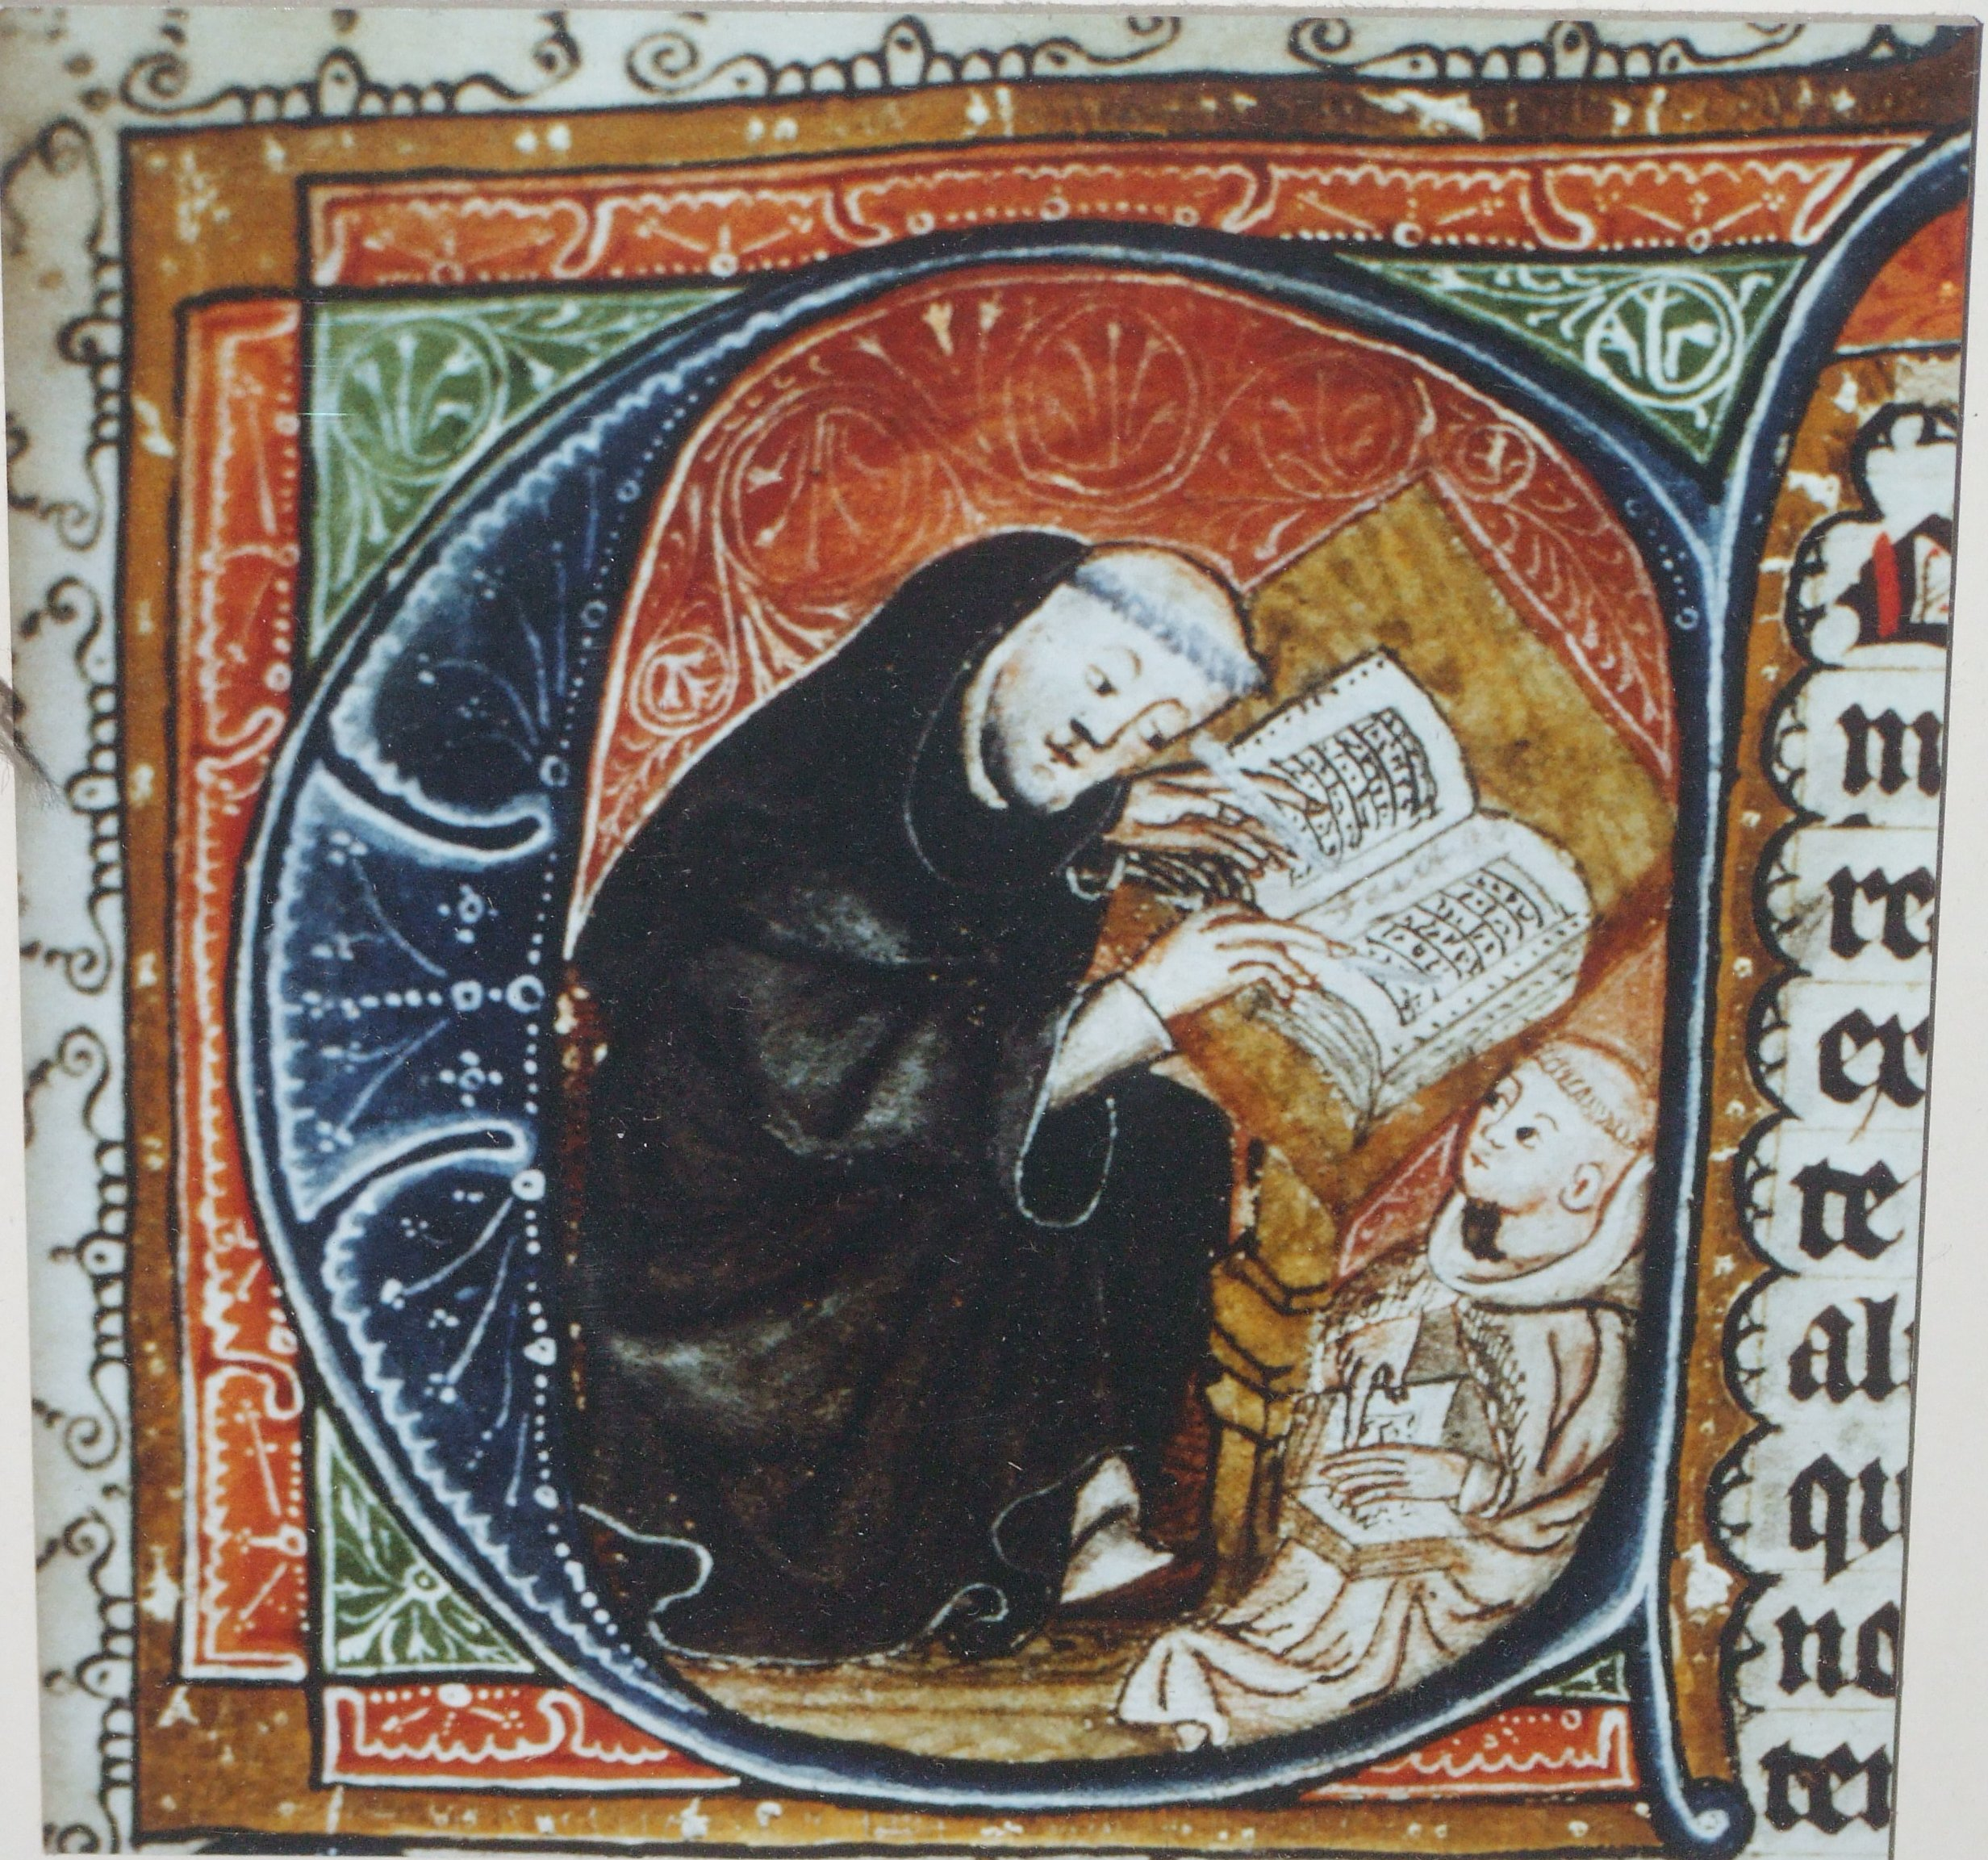
\includegraphics[width=20mm]{Caesarius_von_Heisterbach_als_Novizenmeister}
 \caption{Caesarius v. Heisterbach}
\end{marginfigure}
(inkl. Bildunterschrift) und Tabellen auf den Rand zu platzieren:

\begin{lfgwcode}{}
 \begin{marginfigure}
 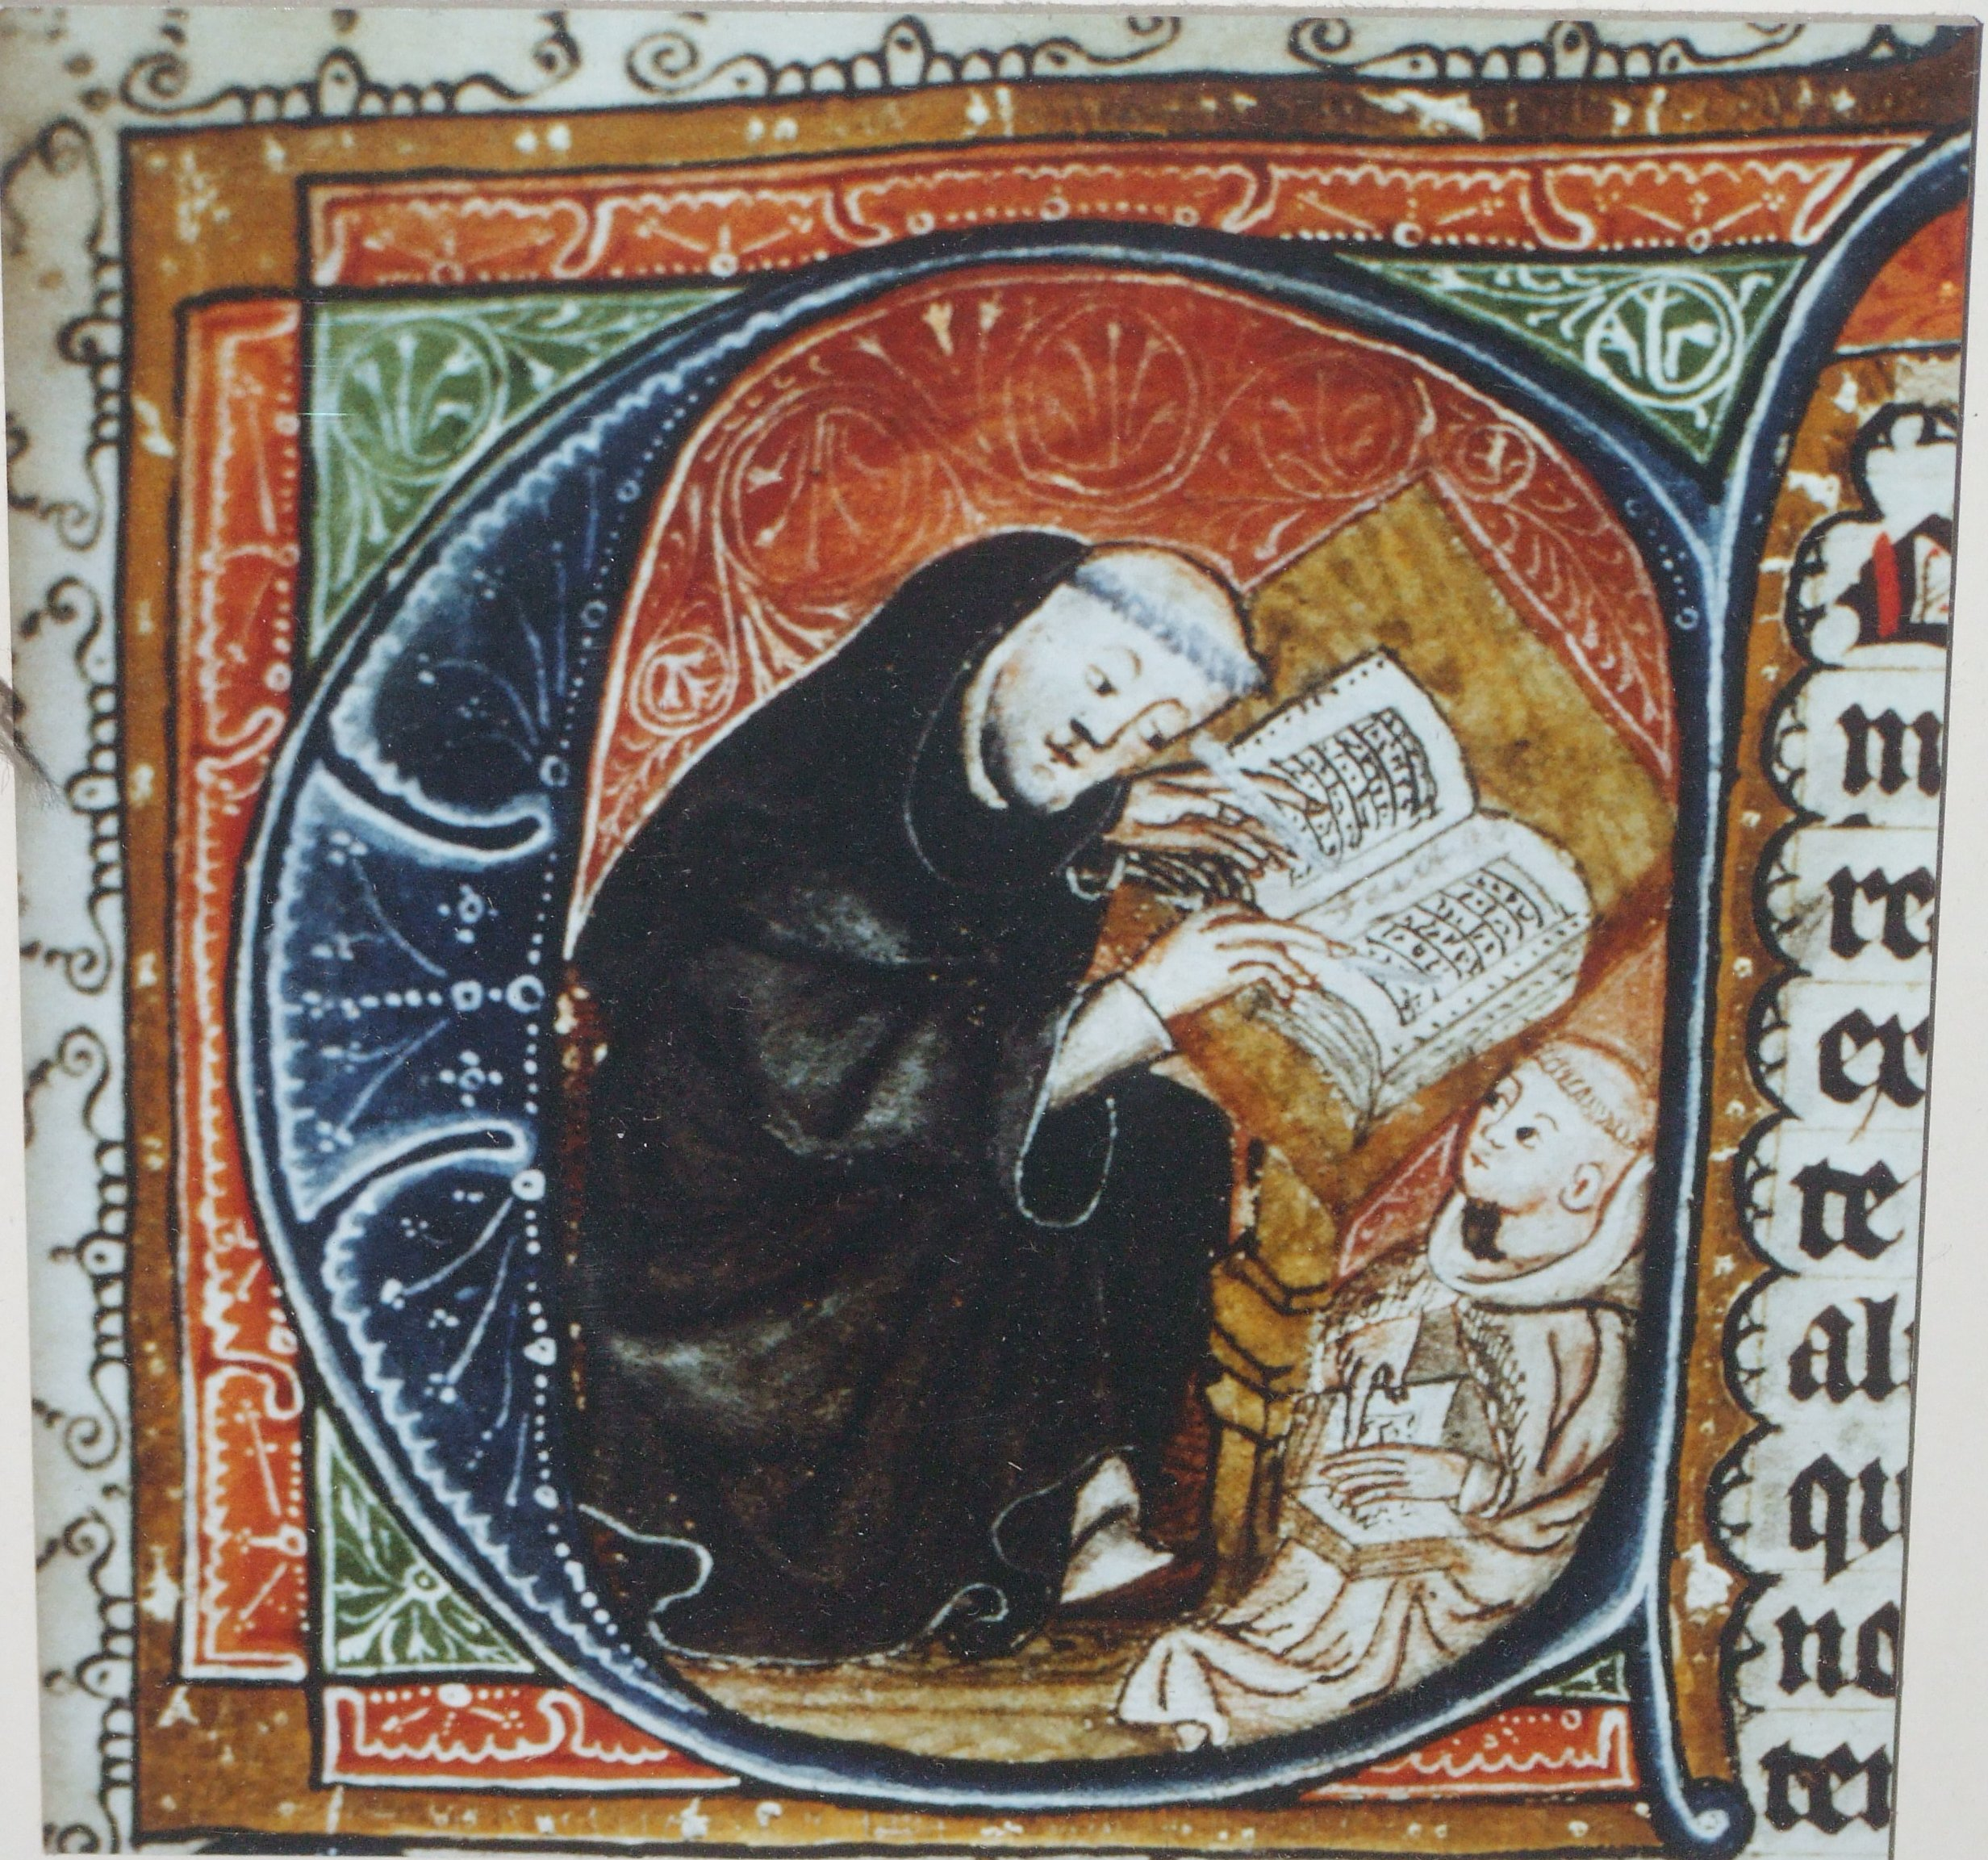
\includegraphics[width=20mm]{Caesarius_von_Heisterbach_als_Novizenmeister}
 \caption{Caesarius v. Heisterbach}
\end{marginfigure}
\end{lfgwcode}


Eine weitere Option ist, die Beschriftung einer Gleitumgebung (Bild, Tabelle) auf den Rand zu
setzen, während die Gleitumgebung selbst die gesamte Breite des Textfeldes einnimmt.

Auch Bilder und Tabellen, die sich über die ganze Seitenbreite, d.\,h. den eigentlichen Satzspiegel
\emph{und} die Marginalspalte erstrecken, werden unterstützt.

Nähere Informationen enthält die Paketdokumentation.


\section{Texte mehrspaltig setzen}

Es gibt in \LaTeX{} zwei verschiedene Wege, zweispaltigen Satz zu erreichen:
Bereits der \LaTeX{}-Kern bietet die Möglichkeit, Texte zweispaltig zu setzen;
daneben gibt es das Paket \paket{multicol}, dass mehrspaltige Einschübe in einem ansonsten
einspaltigen Dokument ermöglicht.

Beide Verfahren haben ihre Berechtigung, denn es ergeben sich jeweils verschiedene
Vor- und Nachteile bzw. Einschränkungen:

\minisec{Das ganze Dokument zweispaltig setzen}

Wird als Dokumentklassen-Option \lstinline/twocolumn/ angegeben, wird das Dokument
zweispaltig gesetzt.
Der Titel mit Datum, Autorangabe, Abstract etc. werden als einspaltiger Kopf über beide
Spalten gesetzt.


\minisec{Zweispaltige Einschübe in einem einspaltigen Dokument I: \LaTeX}

Daneben bietet \LaTeX{} die Möglichkeit, in einem Dokument eine zweispaltige Passage
zu integrieren. Die Passage wird mit dem Befehl \lstinline/\twocolumn[xxx] /
eingeleitet. Die angegebene Überschrift wird einspaltig über beide Spalten gesetzt.
Außer einer echten Überschrift (z.\,B. \lstinline/\section{}/) sind hier auch
längere Einleitungstexte etc. möglich.

Mit dem Befehl \lstinline/\onecolumn/ wird wieder auf einspaltigen Satz zurückgestellt.

Beide Kommandos beginnen jeweils eine neue Seite, was ihre praktische
Benutzbarkeit meines Erachtens nach stark einschränkt.


\minisec{Mehrspaltige Einschübe in einem einspaltigen Dokument II: \paket{multicol}}

\begin{multicols}{2}
 Die umfassendste Funktionalität bietet das Paket \paket{multicol} von Frank Mittelbach.
 Mit ihm lassen sich beliebige Textpassagen in mehreren Spalten in ein ansonsten
 einspaltiges Dokument einfügen.

 Der Beginn einer mehrspaltigen Passage wird durch \lstinline/\begin{multicols}{Zahl}/
 eingeleitet; die entsprechende Anweisung \lstinline/\end{multicols}/ schaltet wieder
 auf einspaltigen Satz um. \lstinline/Zahl/ steht dabei für die Anzahl der gewünschten
 Spalten.
\end{multicols}

\setlength{\columnseprule}{0.4pt}
\begin{multicols}{3}
 Dabei liegt es in der Verantwortung des Nutzers, nicht zu viele Spalten zu verlangen,
 da sonst die einzelnen Spalten zu schmal werden und sich Aussehen und Lesbarkeit erheblich
 verschlechtern.

 Faustregel: Der Wortabstand soll niemals größer sein als der Zeilenabstand.
 Evtl. kann es helfen, mehrspaltige Abschnitte im Flattersatz zu setzen.
 In typografischer Hinsicht ist dies ein sehr schlechter Absatz \dots

 Um dem Leser zu ermöglichen, die Spalten besser wahrzunehmen kann der Längenwert
 \lstinline/columnseprule/ auf einen Wert größer 0 gestellt werden;
 in diesem Beispiel liegt er bei 0.4pt: \lstinline/\setlength{\columnseprule}{0.4pt}/.

 Daneben bietet das Paket weitere Einstellmöglichkeiten, wie. z.\,B. den Spaltenabstand
 oder die Farbe der Trennlinie.
\end{multicols}



\section{Das Konzept der \enquote{Gleitumgebung}}
\dictum[Heraklit?]{Alles fließt.}

\minisec{Gleitumgebungen beschriften: Das Paket \paket{caption}}

\section{Grafiken einbinden}
\label{grafik-einbinden}
\index{Grafik}
\index{Bilder}
\index{Abbildungen}

Voraussetzung: Paket \paket{graphicx} in Dokumentpräambel einbinden:
\lstinline/\usepackage{graphicx}/.

Dann fügt der Befehl \lstinline/\includegraphics[Optionen]{Name}/ an der jeweiligen Stelle
die angegebene Grafik (als eigenen Absatz) ein.
Als Option sollte z.\,B. die gewünschte Abbildungsgröße eingestellt werden.
Wieder sind sowohl absolute Angaben möglich als auch Bezugnahmen z.\,B. auf
\lstinline/\textwidth/.

Meist möchte man die Abbildung jedoch in eine Gleitumgebung einfügen, so dass das Satzprogramm
flexibler die Positionierung entscheiden kann (s. vorheriger Abschnitt).
Dazu dient die Umgebung \lstinline/figure/.
Dann ist auch die Angabe einer Bildunterschrift mit dem Paket \paket{caption} möglich.

Ggf. empfiehlt sich auch noch das Einbetten in eine \lstinline/center/-Umgebung,
um das Bild auf die Mitte des Satzspiegels zu zentrieren.

Alles zusammen sieht dann so aus:

\begin{lstlisting}
\begin{figure}
 \begin{center}
  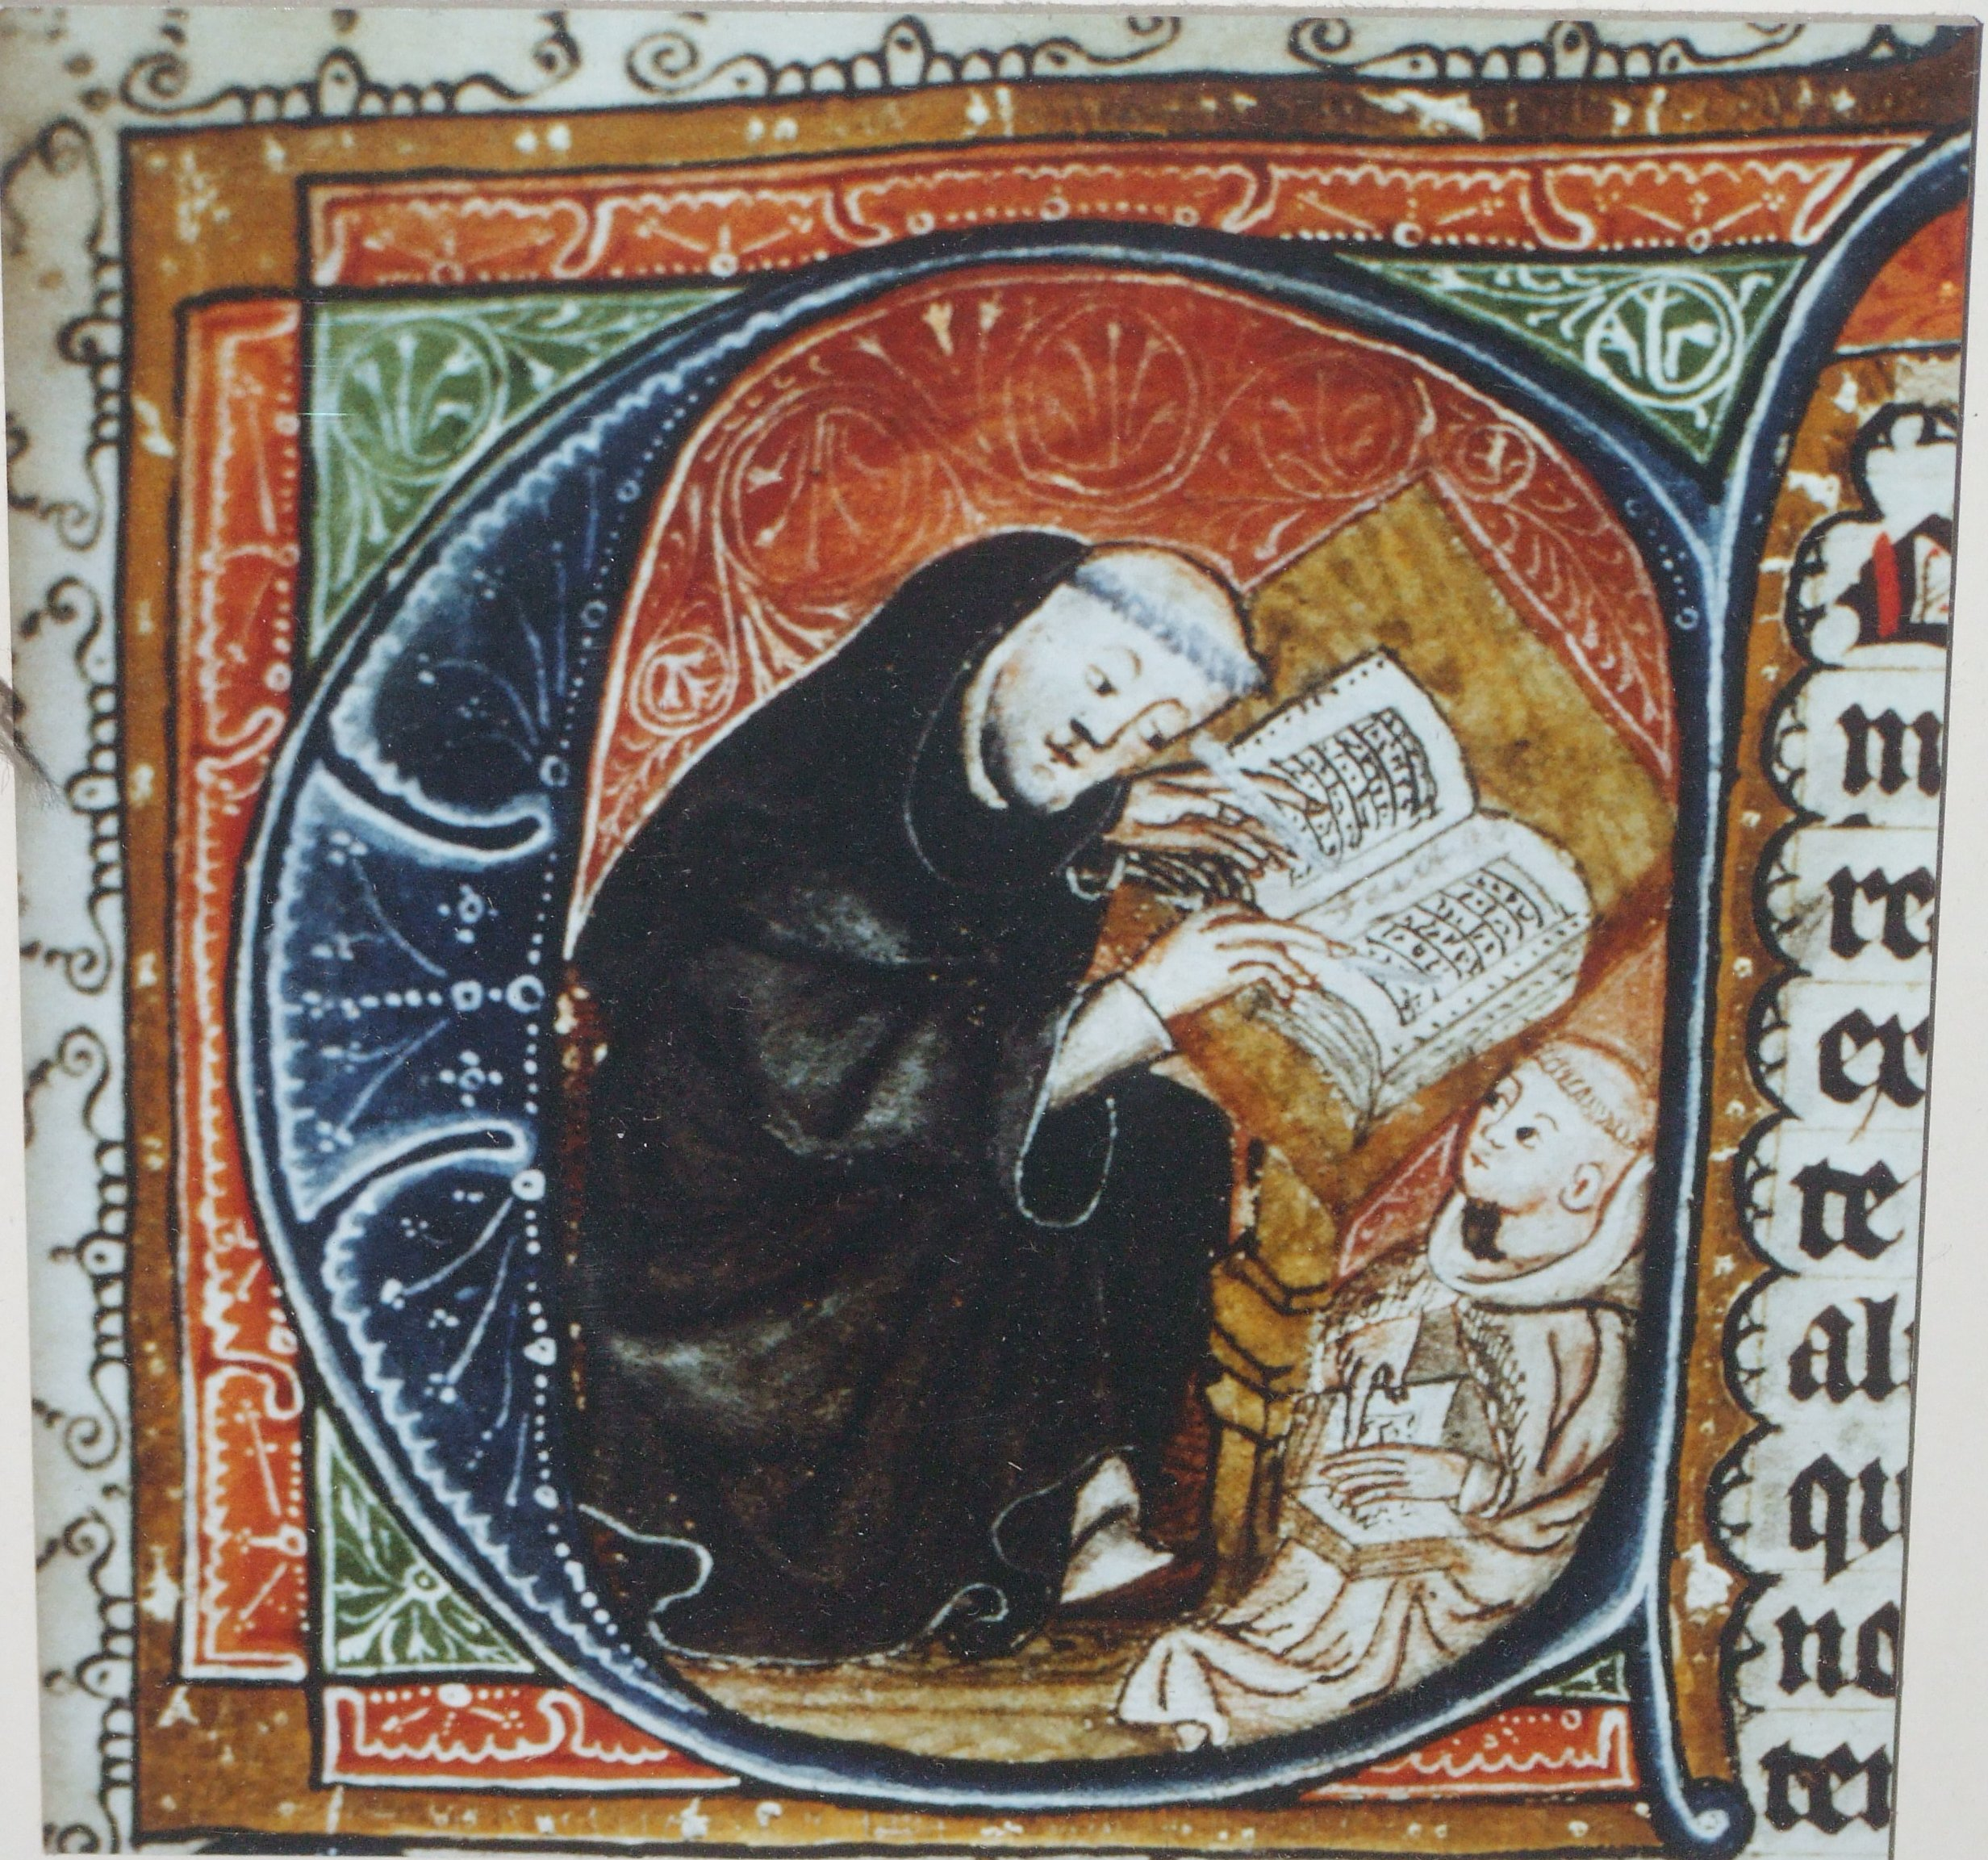
\includegraphics[width=.5\textwidth]{Caesarius_von_Heisterbach_als_Novizenmeister}
  \caption{Caesarius von Heisterbach als Novizenmeister}
 \end{center}
\end{figure}
\end{lstlisting}


\begin{figure}[!htb]
\centering
  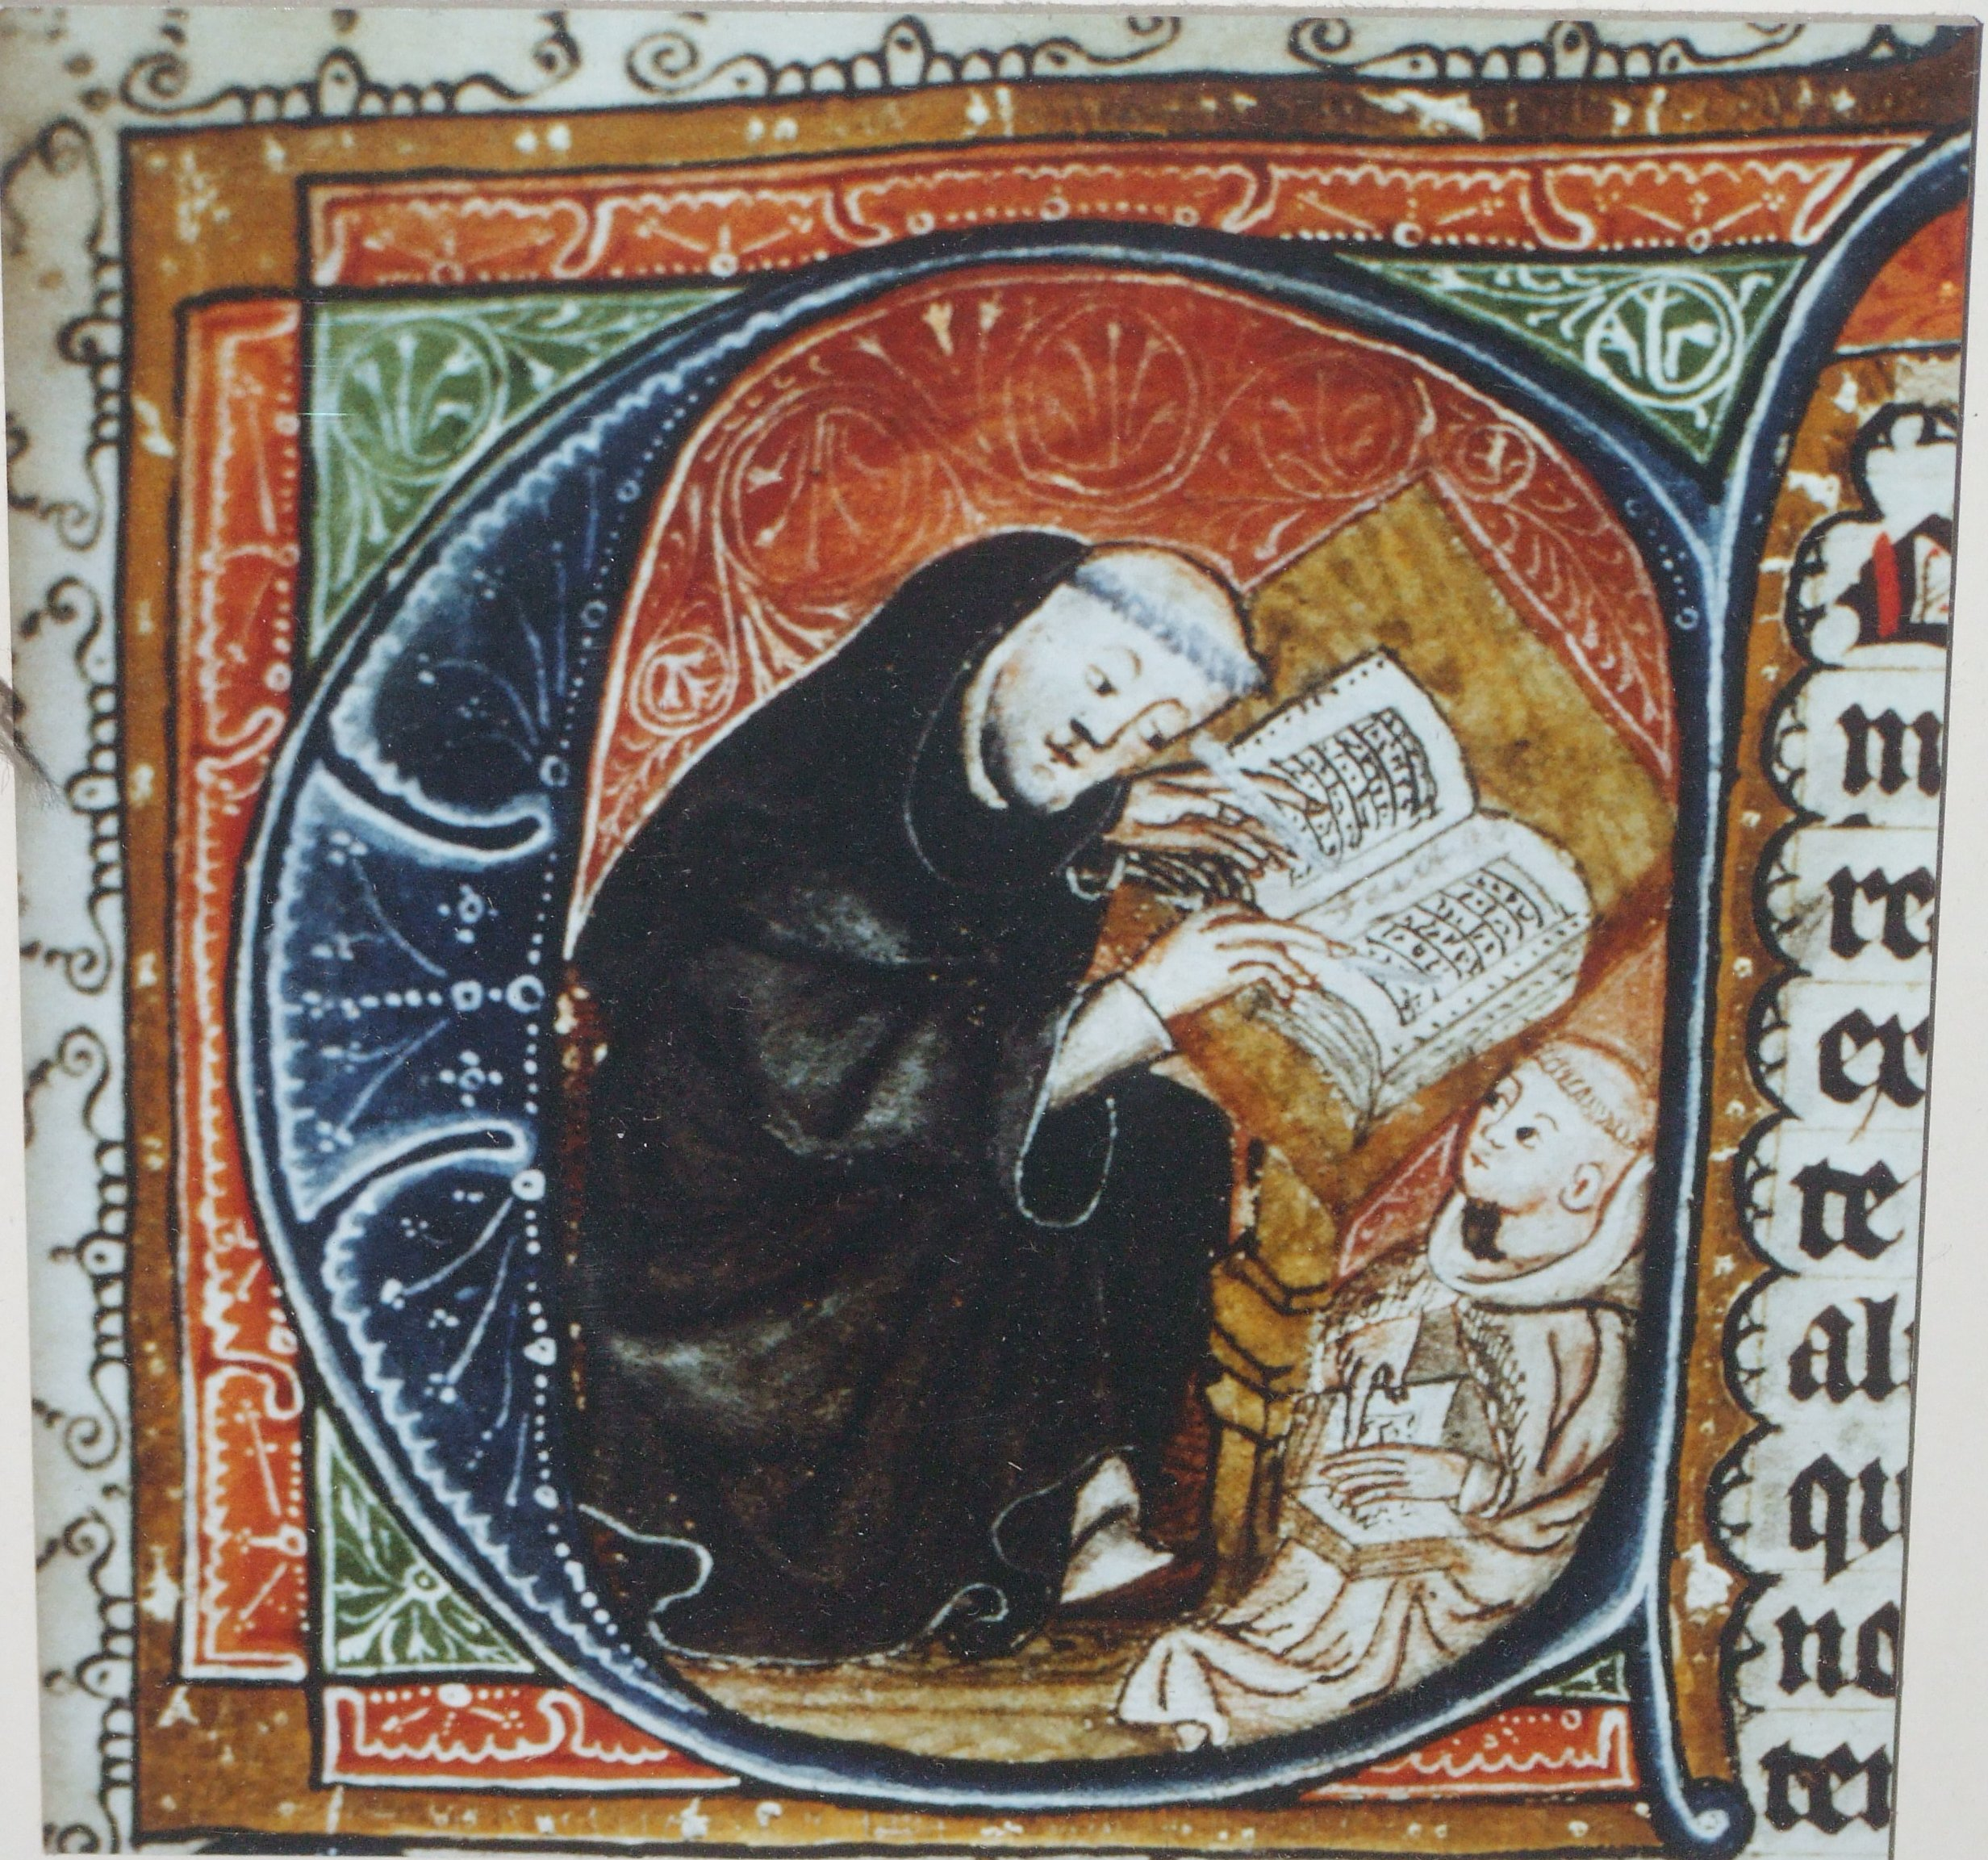
\includegraphics[width=.7\textwidth]{Caesarius_von_Heisterbach_als_Novizenmeister}
  \caption{Caesarius von Heisterbach als Novizenmeister}
\end{figure}

\section{Unter-Abbildungen mit \protect\paket{subcaption}}


\section{Tabellen erstellen}

Komplexes Thema, Spezialliteratur gerechtfertigt.\footcite{voss:tabellen}


\paket{tabularx}

\paket{longtable}

\minisec{Tabellen drehen}
\index{Drehen von Texten}

\paket{rotatebox}


\section{Umgang mit Bibelstellen}
\index{Bibelstellen}

Vor allem im Rahmen größerer Projekte empfiehlt es sich dringend, Bibelstellenangaben nicht einfach
\enquote{frei Hand} in den Text zu schreiben, sondern diese in einer eindeutigen Form
-- mit Hilfe eines \LaTeX{}-Befehls, der auszuzeichnen.
Dafür gibt es zwei Gründe:

\begin{itemize}
    \item Wenn man die Bibelstellenangaben auszeichnet, kann man in seinem Editor rasch alle
    Stellenangaben aufsuchen, etwa um sie nachzuschlagen, auf Vollständigkeit zu überprüfen etc.
    \item Die eindeutige Auszeichnung ist Voraussetzung für eine automatische Erfassung in einem
    Index.
    \item Während der langen Rezeptionsgeschichte der Bibel haben sich verschiedene Standards der
    Bezeichnung der einzelnen biblischen Bücher herausgebildet. Stützt man seine Stellenangaben
    auf eine eindeutig definierte maschinenlesbare Codierung, kann man den Computer automatisch
    dafür sorgen lassen, dass alle Bibelstellenangaben einer bestimmten Wiedergabekonvention folgen.
    Also, dass z.\,B. das erste Buch der Bibel einheitlich entweder als \enquote{Genesis} oder als \enquote{1. Buch Mose}
    referenziert wird.
\end{itemize}

Im Folgenden geht es darum, für die Zitierweise von Bibelstellen eine eindeutige Codierung zu verwenden,
die es einerseits ermöglicht, die auftretenden Bibelstellenangaben eindeutig und automatisch
verarbeitbar zu erfassen.
Andererseits soll die Erfassung möglichst komfortabel sein, das heißt möglichst wenige
kryptische Steuerzeichen in den Text bringen und außerdem in gewissen Grenzen tolerant gegenüber
menschlicher Uneinheitlichkeit und Neigung zu Fehlern sein.

Zweck dieses Codierungsaufwandes ist die einheitliche Formatierung der Bibelstellenangaben
entsprechend etablierter Leitlinien sowie die automatische Erstellung eines Bibelstellenregisters.

Zu diesem Zweck existieren auf \url{https://ctan.org} mehrere Pakete, die den Umgang
auch mit großen Mengen an Bibelstellenangaben sehr komfortabel machen:

\begin{itemize}
    \item \paket{bibleref}
    \item \paket{bibleref-german}
    \item \paket{bibleref-parse}
\end{itemize}

\minisec{Das Paket \paket{bibleref}}

Das Paket \paket{bibleref} von Nicola Talbot bietet die genannten Vorzüge, richtet sich aber primär
an die Bedürfnisse englischsprachiger Nutzer.
Dennoch lohnt sich ein Blick auf das Paket, weil es die konzeptionelle Grundlage für
\paket{bibleref-german} bildet, dessen Funktionsweise man verstanden haben sollte.

\paket{bibleref} stellt hauptsächlich zwei Makros bereit, die zuallererst wichtig sind:

\begin{itemize}
    \item \lstinline/\bibleref { Buch } ( Verse )/ dient zur Angabe einer Bibelstelle.
    Für Buch ist ein definiertes Kürzel einzugeben, dass in der Ausgabe ggf. durch eine vollständigere
    Schreibweise einheitlich ersetzt wird. (Das lässt sich einstellen; verschiedene Stile sind vordefiniert.)
    \item \lstinline/\ibibleref { Buch } ( Verse )/ dito, zugleich wird im Bibelstellenregister (s.u.)
    ein Eintrag vorgenommen.
\end{itemize}

Mit diesen beiden Befehlen lassen sich Bibelstelleneingaben eindeutig bezeichnen und deshalb
mit Programmhilfe einheitlich formatiert ausgeben und im Register erschließen.
Voraussetzung ist natürlich das Einbinden des Paketes in der Präambel:
\lstinline/\usepackage{bibleref}/
Ein Beispiel:

\begin{lfgwcode}{}
Es gibt vier Evangelien:
\ibibleverse{Mt},
\ibibleverse{Mk},
\ibibleverse{Lk} und \ibibleverse{John}.

Diese Stelle kommt nicht ins Register: \bibleverse{Rev}(13:15-17),
während diese dort schon erscheint: \ibibleverse{John}(3:17).
Die Bergpredigt steht übrigens in \ibibleverse{Mt}(5-7:).
\end{lfgwcode}

Die Bearbeitung mit \LaTeX\ führt dazu, dass die Bibelstellen einheitlich formatiert ausgegeben werden:

\begin{quotation}
    Es gibt vier Evangelien: Matthew, Mark, Luke und John.
    Diese Stelle kommt nicht ins Register: Revelation 13:15–17, während diese dort schon
    erscheint: John 3:17. Die Bergpredigt steht übrigens in Matthew 5–7.
\end{quotation}

Doch das Paket hat noch mehr zu bieten:
\paket{bibleref} erlaubt, durch optionale Angabe eines Zitierstiles,%
\footnote{Paketoption \lstinline|biblerefstyle|.}
die Bibelstellen auf verschiedene
Weise auflösen zu lassen:
\lstinline/\usepackage[biblrefstyle=...]{bibleref}/

Zur Wahl stehen angloamerikanische und international verbreitete Zitierstile:

\begin{labeling}{anglosaxon}
    \item[default] 2 Corinthians 12:1-5
    \item[jerusalem] 2 Co 12:1-5
    \item[anglosaxon] II Cor. XII.1-5
    \item[JEH] 2 Cor. xii. 1-5
    \item[NTG] 2 Cor xii, 1-5
    \item[MLA] 2 Cor. xii.1-5
    \item[chicago] 2 Cor. xii: 1-5
    \item[text] Second Epistle to the Corinthians, chapter twelve verse one to five
\end{labeling}

Betrachtet man die entstandene Ausgabe unseres Beispieltextes, so fallen
dem deutschen Leser (mindestens) vier Wünsche ein, die der unmittelbaren Verwendung von
\paket{bibleref} in deutschsprachigen Texten im Wege stehen:

\begin{itemize}
    \item Einzelne Kürzel sind im deutschen Sprachraum unhandlich: \enquote{John} statt \enquote{Jo}.
    (Übrigens: Verwendet man die Abkürzung \enquote{Jo}, wird diese zu \enquote{Joel} expandiert.)
    \item Die in der Ausgabe erzeugten Bezeichnungen der biblischen Bücher sind englisch bzw.
    -- je nach eingestelltem Zitierstil -- lateinisch.
    \item Die Zeichensetzung der ausgegebenen Stellenangaben ist für deutsche Gewohnheiten ungewohnt:
    Wir erwarten statt Angaben wie \enquote{Gen 1:1} eher das Format \enquote{Gen 1,1}:
    Buch -- Kapitel -- Komma -- Vers.
    \item Die Codierung der Versangaben im Quelltext ist etwas unhandlich.
\end{itemize}

Alle vier Einschränkungen lassen sich umgehen;
für die ersten drei Punkte hilft \paket{bibleref-german},
für die letzte Einschränkung wurde \paket{bibleref-parse} entwickelt.
Es ist besonders praktisch, dass sich beide Pakete kombinieren lassen.


\minisec{Das Paket \paket{bibleref-german}}

Das Paket \paket{bibleref-german} wurde von Dr. Dominik Waßenhoven entwickelt und bietet die Leistungen von \paket{bibleref}
angepasst an die Bedürfnisse deutscher Nutzer.

Es stellt im deutschsprachigen Raum das Standardwerkzeug zum Umgang mit Bibelreferenzen dar,
deshalb soll seine Funktionalität etwas genauer demonstriert werden.

Mit Hilfe von \paket{bibleref} erstellte Dokumente sind unverändert lauffähig, wenn man nur
den Paketaufruf austauscht. (Übrigens stehen auch die englischsprachigen Ausgabeformate von
\paket{bibleref} unter \paket{bibleref-german} zur Verfügung.)

Das Ergebnis desselben Eingabetextes wie oben entspricht weit mehr deutschen Erwartungen, wenn man
nur den Paketaufruf in der Präambel ersetzt
(\lstinline/\usepackage{bibleref-german}/): XXXX

\begin{quotation}
    Es gibt vier Evangelien: Matthäus, Markus, Lukas und Johannes.
    Diese Stelle kommt nicht ins Register: Offenbarung 13,15–17, während diese dort schon
    erscheint: Johannes 3,17. Die Bergpredigt steht übrigens in Matthäus 5–7.
\end{quotation}

%\begin{figure}
%\includegraphics[scale=.5]{listing_bibleref-german}
%\caption{Das Ergebnis von Listing 2.}
%\end{figure}

Das Ersetzen von \paket{bibleref} durch \paket{bibleref-german} hat
drei Dinge zur Folge:

\begin{itemize}
    \item Das Paket \enquote{versteht} als Eingabe sowohl die im deutschsprachigen Raum üblichen Kürzel -- übrigens
    auch die englischen -- als auch die ausgeschriebenen Buchnamen. Man braucht keine Namenskonventionen
    zu \enquote{lernen}, meistens versteht biblref-german, welches Buch man meint.
    Teilweise sind mehrere Bezeichnungen für das gleiche Buch definiert -- z.B. sind Numeri, Num, 4Mos und
    IVMos gleichbedeutend.
    (Selbstverständlich enthält die Paketdokumentation eine vollständige Auflistung der Buchbezeichnungen.)%
    \footnote{Achtung! Die Eingabecodierung \enquote{Jo} wird zum Buch Joel aufgelöst; das Johannes-Evangelium
        ist als \enquote{Joh} einzugeben, was dann bei Verwendung des Vulgata-Stils zu Io interpoliert wird.
        So kompliziert kann die Welt sein\ldots }
    \item In der Ausgabe erscheinen deutsche Buchtitel.
    \item Die Zeichensetzung entspricht deutschen Gewohnheiten.
\end{itemize}

Über die Konfigurationsmöglichkeiten des englischsprachigen \paket{bibleref} lässt sich das Ausgabeformat der Bibelstellenangaben bei \paket{bibleref-german} in
zweierlei Weise modifizieren:

\begin{itemize}
    \item Zitierstil:
    Durch die Angabe als Paketoption oder alternativ mit \cs{biblerefstyle\marg{Stil}} lässt sich die Ausgabekonvention verändern.
    Mögliche Werte sind die im deutschsprachigen Raum meist verwendeten Standards:
    \begin{itemize}
        \item \lstinline/Einheitsübersetzung/ (der voreingestellte Standardwert),
        \item \lstinline/Lutherbibel/ (in der Form von 1984),
        \item \lstinline/LThK/ (die Konventionen des Lexikons für Theologie und Kirche),
        \item \lstinline/RGG/ (Religion in Geschichte und Gegenwart),
        \item \lstinline/TRE/ (Theologische Realenzyklopädie) und
        \item \lstinline/Vulgata/ (die lateinischen Bezeichnungen der Vulgata).
    \end{itemize}

    \item Format:
    Für jeden dieser Zitierstile definiert \paket{bibleref-german} noch vier Formate, die die Wiedergabe der
    Stellenangaben definieren und durch den Befehl \lstinline/\biblerefformat{<Format>}/ eingestellt
    werden können:

    \begin{itemize}
        \item kurz -- Offb 13,17
        \item lang -- Offenbarung 13,17
        \item Terminus -- Die Offenbarung des Johannes 13,17
        \item Zahlwort -- Die Offenbarung des Johannes, Kapitel dreizehn, Vers siebzehn
    \end{itemize}

\end{itemize}

Mit beiden Angaben lässt sich die Ausgabe der Belege sehr differenziert an die eigenen Bedürfnisse
anpassen:

%\lstinputlisting[caption=Beispiel 3: Die selbe Stelle in verschiedenen Formaten und Stilen]
%    {listing_bibleref-german_stile}

\begin{lstlisting}
\documentclass{scrartcl}
\usepackage[utf8]{inputenc}
\usepackage[T1]{fontenc}
\usepackage[ngerman]{babel}

\usepackage{bibleref-german}

\begin{document}
\bibleverse{Jo}(1:1)

\bibleverse{Joh}(3:17)

\biblerefstyle{Vulgata}
\bibleverse{Offb}(1:1)

\biblerefformat{lang}
\bibleverse{Offb}(1:1)

\biblerefstyle{LThK}
\bibleverse{Joh}(3:17)

\biblerefformat{Terminus}
\bibleverse{Joh}(3:17)

\biblerefformat{Zahlwort}
\bibleverse{Joh}(3:17)

\biblerefstyle{Vulgata}
\biblerefformat{kurz}
\bibleverse{Joh}(1:1)
\end{document}
\end{lstlisting}

Es ergibt sich eine erstaunliche Variationsbreite an Zitiermöglichkeiten:

\begin{quotation}
    Joël 1,1

    Johannes 3,17

    Apc 1,1

    Apocalypsis 1,1

    Johannes 3,17

    Das Evangelium nach Johannes 3,17

    Das Evangelium nach Johannes, Kapitel drei, Vers siebzehn

    Io 1,1
\end{quotation}


Die Formate Terminus und Zahlwort sind im Deutschen wegen der notwendigen Flexion der bestimmten Artikel
problematischer als die englischsprachigen \texttt{text}-Variante des Paketes \paket{bibleref}.
Ihre Benutzung ist wahrscheinlich eher die Ausnahme.
Anzumerken ist, dass der Stil Zahlwort ausgaben wie ``Kapitel one'' ergibt, wenn nicht mit babel
die Sprache auf german (oder ngerman) eingestellt wurde. Das Babel-Paket muss vor bibleref-german
eingebunden werden.

Selbstverständlich muss der verantwortungsbewusste Textautor selbst entscheiden, in welchem Maße
das Vermischen verschiedener Formate und insbesondere Stile innerhalb eines Dokumentes sinnvoll ist.

Mit \paket{bibleref-german} lassen sich die deutschsprachigen Gepflogenheiten bei der Formatierung von
Bibelstellenangaben sehr präzise abbilden. Wenn jetzt noch das Eingabeformat (hinsichtlich Kapitel- und
Versangabe) etwas handlicher wäre \dots


\subsection{Das Paket \paket{bibleref-parse}}

Genau dies ist das Ziel des Paketes \paket{bibleref-parse} von Sebastian Kuhnert:
\enquote{The bibleref-parse package parses Bible passages that are given in a human readable format.}
\footnote{Sebastian Kuhnert, The bibleref-parse Package, S. 1}
Die beiden wichtigsten Befehle, die von dem Paket definiert werden, lauten analog zu
\paket{bibleref} und \paket{bibleref-german}:

\begin{itemize}
    \item\lstinline/\pbibleref { Buch mit Kapitel- u. Versangabe } / (Man beachte das \textbf{p}!)
    \footnote{Die Umbenennung der beiden Befehle ist deshalb nötig, weil innerhalb desselben
        Dokuments sowohl Bibelstellen im Eingabeformat von \paket{bibleref} bzw. \paket{bibleref-german} als auch
        im Format von \paket{bibleref-parse} möglich sind. Wahrscheinlich ist es empfehlenswert, bei einer größeren
        Arbeit sich auf \paket{bibleref-parse} festzulegen und eine eigene Abkürzung zu definieren, z.B.
        \lstinline/bibel/ für normale Stellen und \lstinline/bibelx/ für Stellen, die im Index
        erfasst werden sollen.}
    definiert einen Bibelstellenverweis.
    \item\lstinline/\pibibleref { Buch mit Kapitel- u. Versangabe } / (nicht vergessen: \textbf{p}!) dito, zugleich wird im Bibelstellenregister (s.u.)
    ein Eintrag vorgenommen.
\end{itemize}

Mit ihnen ist es möglich, Bibelstellen so zu zitieren, wie es der deutschsprachige Nutzer gewohnt ist.
Dabei stellt sich der Parser sehr weitgehend auf die vielen Sonderfälle ein, die in Bibelstellen
auftreten können. Deshalb ist die Hauptregel ganz einfach:
\enquote{The  basic message is: Just use your intuition. This is what this package was created for.}%
\footnote{ebd. S. 3.}

Diese Erklärung verspricht nicht zuviel, wie das folgende Listing zeigt:
bibleref-parse in Zusammenspiel mit biblref-german:
Bequemer geht's nicht. Nur das \enquote{p} am Beginn der Bibelstellen-Kennungen darf man nicht vergessen\ldots

%\lstinputlisting[caption=Beispiel 4: bibleref-parse in Zusammenspiel mit biblref-german:
%    Bequemer geht's nicht. Nur das ``p'' am Beginn der Bibelstellen-Kennungen darf man nicht vergessen...]
%    {listing_bibleref-german-parse}

\begin{lstlisting}
\documentclass{scrartcl}
\usepackage[utf8]{inputenc}
\usepackage[T1]{fontenc}

\usepackage{bibleref-german} % Ausgabe: deutsche Gepflogenheiten
\usepackage{bibleref-parse}  % Eingabe: quasi künstliche Intelligenz ;-)


\begin{document}
Es gibt vier Evangelien:
\pibibleverse{Mt},
\pibibleverse{Markus},
\pibibleverse{Luke}
und \pibibleverse{Joh}.
Diese Stelle kommt nicht ins Register: \pbibleverse{Offb 13,15-17},
während diese dort erscheint: \pibibleverse{Joh 3,17}.
Die Bergpredigt steht übrigens in \pibibleverse{Mt 5-7}.
\end{document}
\end{lstlisting}

%\begin{figure}
%\includegraphics[scale=.5]{listing_bibleref-german-parse}
%\caption{Das Ergebnis von Listing 4.}
%\end{figure}

Nur der Vollständigkeit halber die \enquote{Auflösung} durch \LaTeX\ldots

\begin{quotation}
    Es gibt vier Evangelien: Matthäus, Markus, Lukas und Johannes. Diese Stelle kommt
    nicht ins Register: Offenbarung 13,15–17, während diese dort erscheint: Johannes 3,17.
    Die Bergpredigt steht übrigens in Matthäus 5–7.
\end{quotation}

Die Aufgabenstellung, unter Benutzung einer leicht handhabbaren, \enquote{menschenfreundlichen} Codierung
Bibelstellenangaben mit computerischer Einheitlichkeit auszugeben -- und das auch noch in verschiedenen
vordefinierten Stilen -- ist mit Hilfe von \paket{bibleref-german} und \paket{bibleref-parse} gelöst.

Damit ist zugleich die Voraussetzung für die ebenso mühelose Erstellung eines Bibelstellenindex geschaffen.

Zur Registererstellung vgl. \fullref{Bibelstellenregister}.


% Section Lyrik-Satz von Christine Römer - thm 6.3.2017

%% lfgw: 2.19 Lyrik-Satz


%% !TEX root = lfgw.tex

\RequirePackage{iftex}
\RequireLuaTeX
\RequirePackage{luatex85}

\documentclass[%
   ibycus,polutonikogreek,english,french,latin,ngerman,%global definiert!
   %%%draft=false,%
   fontsize=11pt,%
   paper=17cm:24cm,%
   DIV=13,%
   listof=totoc,%
   bibliography=totoc,%
   pagesize%
   ]{scrbook}

\KOMAoption{bibliography}{leveldown}

\usepackage{yfonts}
\usepackage{textgreek}
\usepackage{cjhebrew}[2017/03/06]
\usepackage{amsmath,amssymb} % für forrest
%%%\usepackage{textcomp}
\usepackage{unicode-math}
\usepackage{fontspec}
\defaultfontfeatures{Ligatures=TeX,Scale=MatchLowercase}
%\newfontfamily\GFSDidot{GFS Didot}
\newcommand\gkk[1]{%{\GFSDidot
#1}

\usepackage[]{babel}
%\usepackage[ngerman,noftligs]{selnolig}
%%%\setmainfont{Libertinus Serif} %reicht auch, unten evtl. besser wegen SB
\setmainfont{libertinusserif}[
   Extension = {.otf},
   UprightFont = {*-regular}, ItalicFont = {*-italic},
   BoldFont = {*-bold}, BoldItalicFont = {*-bolditalic},%
   FontFace = {sb}{\updefault}{*-semibold},%
   FontFace = {sb}{it}{*-semibolditalic}]%
\setsansfont{Libertinus Sans}
\setmonofont[Scale=MatchLowercase,FakeStretch=0.85]{DejaVu Sans}%das wird für Griechisch in Codebeispielen gebraucht
\setmathfont{Libertinus Math}
\makeatletter
\newcommand*\sustyle{\addfontfeatures{VerticalPosition=Superior}}
\DeclareTextFontCommand{\textsu}{\sustyle}
\def\@makefnmark{\hbox{\sustyle\@thefnmark}}
\makeatother
\DeclareTextCommandDefault{\textborn}{{\char"002A}}
\DeclareTextCommandDefault{\textdied}{{\char"2020}}
\usepackage[% microtype
   final,%
   tracking=smallcaps,%
   expansion=alltext,%
   protrusion=true%
   ]{microtype}%
\SetTracking{encoding=*,shape=sc}{50}%
\UseMicrotypeSet[protrusion]{basicmath} % disable protrusion for tt fonts

\usepackage[headsepline]{scrlayer-scrpage}
\clearscrheadfoot
\ihead{\headmark}
\ohead{\pagemark}
\pagestyle{scrheadings}

\usepackage[autostyle]{csquotes}
\usepackage[newcommands]{ragged2e}

\usepackage{graphicx}
\graphicspath{{bilder/}}

\usepackage{grffile}
\usepackage[a4,center,cross]{crop}

\usepackage{listings}
\lstdefinestyle{listinglfgw}{%
  inputencoding=utf8,
  extendedchars=true,
  language=[LaTeX]{TeX},
  numbers=left, 
  %stepnumber=3,
  numbersep=5pt, 
  numberfirstline=false,  
  numberstyle=\tiny\textsf,
  basicstyle=\ttfamily\footnotesize,
  keywordstyle=\bfseries,%
  texcsstyle=*\ttfamily\footnotesize\bfseries,%
  %frame=tlrb,
  breaklines=true,
  breakatwhitespace=true,
  breakindent=5pt,
  %postbreak=\mbox{$\hookrightarrow$},
  escapeinside={*@}{@*},
  %showstringspace=false, 
  captionpos=b,
  upquote=true,
  %%%classoffset=0,
  morekeywords={%
  %a
  addbibresource,addplot,Afootnote,alteSeite,autocite,autopar,answerline,alertblock,
  %b
  beginnumbering,Bfootnote,biblerefformat,biblerefmap,biblerefstyle,bonuspointpoints,bibleref,block,
  %c
  Cfootnote,chapter,chbpword,chpword,chpgword,chqword,chsword,chtword,citeauthor,cites,citetitle,columnrulewidth,Columns,columnsposition, center,
  chronology,columns,
  %d
  draw,dictum,deffootnote,deffootnote,description,
  %e
  edtext,endnumbering,enquote,enumi,example,exampleblock,
  %f
  firstlinenum,firstlinenumR,firstpageheadrule,footcite,footcites,footfullcite,fullcite,fillwithgrid,fillwithlines,fillwithdottedlines,Forest,Forest*,
  footnotemargin,fillwithlines, fillwithgrid,
  %h
  hpword,hqword,hsword,htword,hypertarget,hyperlink,hideallsubsection,
  %i
  includegraphics,includeonlyframes,ibibleref,invisible,
  %l
  Lcolwidth,ledsidenote,lemma,linenumincrement,linenumincrementR,
  %m
  msdata,mode,maketitle,multifootsep,
  %n
  newfontface,newfontfamily,node,
  %o
  only,onslide,
  %p
  Pages,parencite,parencites,part,pend,pibibleverse,pbibleverse,pointpoints,printbibheading,printbibliography,printindex,pstart,pgfimage,pgfusepath,
  pgfplothandlerlineto,pgfplotsset,pgfplotxyfile,pbibleref,pibibleref,pgf-pie,plain,
  %q
  quell,question,quote,quotaion,
  %r
  Rcolwidth,reledmac,
  %s
 selectlanguage,setlength,setmainfont,setmonofont,setmsdatalabel,setromanfont,setsansfont,smartcite,smartcites,solutiontitle,setbeamerfont,setbeamercovered,subsection,subsection*,subsubsection,subtitle,solution,solutionorgrid,
  %t
  text,textborn,textcite,textcites,textdelta,textDelta,textdied,texteuro,textgamma,textGamma,textmarried,textsubscript,thealteSeite,tableofcontents,th,TH,
  textalpha, textbeta, textgamma, textdelta, textepsilon, textzeta, texteta, texttheta, textiota, textkappa, textlambda, textmu, textnu,
  textxi, textomikron, textpi, textrho, textsigma, texttau, textupsilon, textphi, textchi,  textpsi, textomega,
  textAlpha, textBeta, textGamma, textDelta, textEpsilon, textZeta, textEta, textTheta, textIota, textKappa, textLambda, textMu, textNu,
  textXi, textOmikron, textPi, textRho, textSigma, textTau, textUpsilon, textPhi, textChi,  textPsi, textOmega, twocolumn,
  %u
  usetheme,usecolortheme,usebackgroundtemplate,useforestlibrary,usepackage,usetikzlibrary,
  %v
  vari,verse,
  %x
  Xafternumber,Xarrangement,Xlemmaseparator,Xinplaceoflemmaseparator,Xinplaceofnumber,Xnonbreakableafternumber,Xnotenumfont,Xnumberonlyfirstinline,Xnumberonlyfirstintwolines,Xsymlinenum,Xtwolines,Xtwolinesbutnotmore,Xtxtbeforenotes
  },   
  literate=
  {á}{{\'a}}1 {é}{{\'e}}1 {í}{{\'i}}1 {ó}{{\'o}}1 {ú}{{\'u}}1
  {Á}{{\'A}}1 {É}{{\'E}}1 {Í}{{\'I}}1 {Ó}{{\'O}}1 {Ú}{{\'U}}1
  {à}{{\`a}}1 {è}{{\`e}}1 {ì}{{\`i}}1 {ò}{{\`o}}1 {ù}{{\`u}}1
  {À}{{\`A}}1 {È}{{\'E}}1 {Ì}{{\`I}}1 {Ò}{{\`O}}1 {Ù}{{\`U}}1
  {ä}{{\"a}}1 {ë}{{\"e}}1 {ï}{{\"i}}1 {ö}{{\"o}}1 {ü}{{\"u}}1
  {Ä}{{\"A}}1 {Ë}{{\"E}}1 {Ï}{{\"I}}1 {Ö}{{\"O}}1 {Ü}{{\"U}}1
  {â}{{\^a}}1 {ê}{{\^e}}1 {î}{{\^i}}1 {ô}{{\^o}}1 {û}{{\^u}}1
  {Â}{{\^A}}1 {Ê}{{\^E}}1 {Î}{{\^I}}1 {Ô}{{\^O}}1 {Û}{{\^U}}1
  {œ}{{\oe}}1 {Œ}{{\OE}}1 {æ}{{\ae}}1 {Æ}{{\AE}}1 {ß}{{\ss}}1
  {ç}{{\c c}}1 {Ç}{{\c C}}1 {ø}{{\o}}1 {å}{{\r a}}1 {Å}{{\r A}}1
  {€}{{\EUR}}1 {£}{{\pounds}}1
}
\lstset{style=listinglfgw}
  
\usepackage[% tcolorbox
  skins,%
  listings,%
  breakable,%
]{tcolorbox}
\tcbset{%
lfgwstyle/.style={%
    before skip=\baselineskip,
    boxrule=0pt,
    %bottomrule=2pt,
    %toprule=2pt,
    %colframe=black,
    colback=black!5,
    coltitle=white,
    bicolor,
    sharp corners,
    colbacklower=white,
    fonttitle=\sffamily\bfseries,
    breakable,
    %label=#1,
}}


\newtcblisting[auto counter,number within=chapter]{lfgwexample}[1]{%
    lfgwstyle,
    fontupper=\small\ttfamily,
    sidebyside,
    listing and text,
    title={Beispiel \thetcbcounter},
    listing options={style=listinglfgw},
    #1,
%text and listing,
}

\newtcblisting[use counter from=lfgwexample,number within=chapter]{lfgwcode}[1]{%
    lfgwstyle,
    fontupper=\small\ttfamily,
    listing only,
    title={Beispiel \thetcbcounter},
    listing options={style=listinglfgw},
    #1,
}

\newtcblisting[use counter from=lfgwexample,number within=chapter]{lfgwprint}[1]{%
    fontupper=\small,
    lfgwstyle,
    text only,
    title={Beispiel \thetcbcounter},
    listing options={style=listinglfgw},
    #1,
}


\usepackage{showexpl}
%\lstset{explpreset={escapeinside={*@}{@*}}}

\usepackage[pagewise]{lineno}
\usepackage{sidenotes}
\usepackage{multicol}
% Für den Abschnitt über Konstituentenanylyse von C. Römer:
\usepackage[linguistics]{forest}
\forestapplylibrarydefaults{linguistics,edges}
\useforestlibrary{edges}
\makeatletter
\let\pgfmathModX=\pgfmathMod@
\usepackage{pgfplots}%
\pgfplotsset{compat=1.14}
\let\pgfmathMod@=\pgfmathModX
\makeatother
%http://tex.stackexchange.com/questions/328972/presence-of-pgfplots-package-breaks-forest-environment-%w-folder-option-en/329015

% Pakete im Bereich Kapitel 3 - Diagramme zeichnen
\usepackage{tikz}
\usepackage[all]{genealogytree}
\usepackage{chronology}
\usepackage{pgf-pie}
\usetikzlibrary{pgfplots.dateplot}
\usetikzlibrary{mindmap}

\deffootnote[1.5em]{1.5em}{1.5em}{\makebox[1.5em][l]{{\fontseries{sb}\selectfont\thefootnotemark\ }}}

\usepackage{enumitem}			% for simple list modifications
\setlist{leftmargin=*,before=\setlength{\rightmargin}{\leftmargin}}

%\usepackage{parallel}


%- Für Lyrik-Satz, Christine Römer:
\usepackage{verse}
\newcommand\He{\textbackslash\xspace}
\newcommand\Se{$\cup$\xspace} 
\newcommand*{\Zr}{\unskip\textunderscore}
\newcommand\daktylus{\textbackslash$\cup\cup$\xspace} 
\newcommand\anapaest{$\cup\cup$\textbackslash\xspace}

% ------------
\usepackage{runic}
\usepackage{hieroglf}
\usepackage[normalem]{ulem} %%% MS: Wofür? Unterstreichungen sollten vermieden werden! LCB: kann \xout
%\usepackage{letterspace} %%% MS: Wofür. Besser direkt \textls aus dem Microtypepaket
%% ------------------------------------------------------------------------
%%   This is a stand-alone version that only provides the letterspacing
%%   commands. Do not use this package together with the `microtype' package.
%%   Please refer to section 7 of the `microtype' documentation.
%% ------------------------------------------------------------------------ 
\usepackage[hyphens]{url}
\usepackage{hologo}
\usepackage{philex}
\def\fg{}
\usepackage{siunitx} %Supreme typesetting of units
%\sisetup{%
%    tight-spacing=true, %
%    %math-rm=\mathsf, 
%    %		text-rm=\sffamily,
%    detect-all, %Zahlen werden in der aktuellen Schrift angezeigt
%    detect-family,
%    exponent-to-prefix  	= true,%
%    round-mode          	= places,% 
%    round-precision     	= 2,%
%    group-minimum-digits 	= 4, % Für "Tausenderpunkt" --> 1.234 anstatt 1234
%    group-separator			={.},% für "12.345" statt "12 345"
%    %  scientific-notation = engineering, % Use multiples of 3 as exponent
%    locale					=DE, % Typeset numbers and units the German way
%    range-phrase 			={$\times$},%
%    %		zero-decimal-to-integer,%aus "2.0" wird "2"
%    range-units				=single,  % --> 2 x 2 m, - auskommentieren für 2 m x 2 m
%    %%%---------
%%    unit-color=myred,
%}

\usepackage[german]{keystroke}% Computer-Tastatur-Tasten in Anweisungs-Texte zu setzen (z.B. \Shift, \Ctrl, \Spacebar).

\usepackage{imakeidx}
\indexsetup{level = \subsection*, toclevel = subsection, noclearpage, headers = {\indexname}{\indexname}}
\makeindex[                title = {Allgemeiner Index}]
\makeindex[name = pakete,  title = {Verzeichnis der Paketnamen}]
\usepackage[% biblatex
   style=authoryear,  
%  style=historische-zeitschrift, % das am liebsten - aber der geht (bei mir?) nicht!
%  pageref=true,
	backend=biber
	]{biblatex}
\addbibresource{lfgw-bibliographie.bib}
%%%\defbibheading{bibliography}{\addchap{#1}} %%%Besser bei \addchap bleiben

\usepackage{fancyvrb}
\makeatletter
\usepackage[% reledmac
   series={A,B,C},%nur die Apparate A B C aktivieren
   noend,%keine Endotenapparate
   noeledsec%keine eledsections et al.
   %noledgroup%keine ledgroups -- das muss hier auskommentiert werden, damit die minipages funktionieren!
]{reledmac}%
\@ifpackagelater{reledmac}{2017/03/20}{%
   % Package is new enough
}{%
\PackageError{reledmac}{Es wird reledmac >= 2.18.1 benötigt.}%
}
\makeatother
\usepackage{reledpar}

\usepackage{varioref}
\usepackage{hyperxmp}
\usepackage{hyperref}
\hypersetup{					% setup the hyperref-package options
	pdftitle={LaTeX für Geisteswissenschaftler},	% 	- title (PDF meta)
	pdfsubject={Handbuch},% 	- subject (PDF meta)
	pdfauthor={varia},	% 	- author (PDF meta)
	pdfauthortitle={},
	pdfcopyright={Copyright (c) \the\year\. All rights reserved.},
	pdfhighlight=/N,
	pdfdisplaydoctitle=true,
	pdfdate={\the\year-\the\month-\the\day}
	pdflang={de},
   pdfencoding=unicode,   % Sorgt für korrekte Umlaute in den pdf-Lesezeichen - thm
	pdfcaptionwriter={varia},
	pdfkeywords={{LaTeX}, {Geisteswissenschaften}},
	pdfproducer={LuaLaTeX},
	pdflicenseurl={http://creativecommons.org/licenses/by-nc-nd/4.0/},
	plainpages=false,			% 	- 
   colorlinks   = true, %Colours links instead of ugly boxes
   urlcolor     =  blue!50!black, %Colour for external hyperlinks
   linkcolor    = blue, %Colour of internal links
   citecolor   = green!50!black, %Colour of citations
   linktoc=page,
  	pdfborder={0 0 0},			% 	-
	breaklinks=true,			% 	- allow line break inside links
 %   bookmarks=true,
	bookmarksnumbered=true,		%
	bookmarksopenlevel=2,
	bookmarksopen=true,		%
   bookmarksdepth=3,
   pdfdisplaydoctitle,
	final=true	% = true, nur bei web-Dokument!! (wichtig!!)
}
\usepackage{bookmark}%advanced bookmarks
\usepackage[% cleveref
  sort,
  nameinlink
  ]{cleveref}%nach hyperref laden

\crefname{tcb@cnt@lfgwexample}{Beispiel}{Beispiele}
\addto\captionsngerman{%
    \crefformat{lfgwexample}{#2Beispiel\,#1#3}%
    \crefformat{lfgwcode}{#2Beispiel\,#1#3}%
    \crefformat{lfgwprint}{#2Beispiel\,#1#3}%
}

\setkomafont{pagehead}{\normalcolor\normalfont\small\upshape}
\setkomafont{pagenumber}{\normalcolor\normalfont\normalsize\bfseries}

\renewcommand*{\glqq}{\textquotedblleft}
\renewcommand*{\grqq}{\quotedblbase}

\providecommand*{\reledmac}{\mbox{\Package{reledmac}}\xspace}

\providecommand*{\LaTeXTeX}{\hologo{(La)TeX}}
\providecommand*{\AmSLaTeX}{\hologo{AmSLaTeX}}
\providecommand*{\AmSTeX}{\hologo{AmSTeX}}
\providecommand*{\biber}{\hologo{biber}}
\providecommand*{\BibTeX}{\hologo{BibTeX}}
\providecommand*{\BibTeXacht}{\hologo{BibTeX8}}
\providecommand*{\ConTeXt}{\hologo{ConTeXt}}
\let\context\ConTeXt
\providecommand*{\emTeX}{\hologo{emTeX}}
\providecommand*{\eTeX}{\hologo{eTeX}}
\providecommand*{\ExTeX}{\hologo{ExTeX}}
\providecommand*{\HanTheThanh}{\hologo{HanTheThanh}}
\providecommand*{\iniTeX}{\hologo{iniTeX}}
\providecommand*{\KOMAScript}{\hologo{KOMAScript}}
\providecommand*{\LaTeX}{\hologo{LaTeX}}
\providecommand*{\LaTeXe}{\hologo{LaTeX2e}}
\providecommand*{\LaTeXIII}{\hologo{LaTeX3}}
\providecommand*{\LaTeXML}{\hologo{LaTeXML}}
\providecommand*{\LuaLaTeX}{\hologo{LuaLaTeX}}
\let\lualatex\LuaLaTeX
\providecommand*{\LuaTeX}{\hologo{LuaTeX}}
\let\luatex\LuaTeX
\providecommand*{\LyX}{\hologo{LyX}}
\providecommand*{\METAFONT}{\hologo{METAFONT}}
\let\MF\METAFONT
\providecommand*{\MetaFun}{\hologo{MetaFun}}
\providecommand*{\METAPOST}{\hologo{METAPOST}}
\providecommand*{\MetaPost}{\hologo{MetaPost}}
\let\MP\METAPOST
\providecommand*{\MiKTeX}{\hologo{MiKTeX}}
\providecommand*{\NTS}{\hologo{NTS}}
\providecommand*{\OzMF}{\hologo{OzMF}}
\providecommand*{\OzMP}{\hologo{OzMP}}
\providecommand*{\OzTeX}{\hologo{OzTeX}}
\providecommand*{\OzTtH}{\hologo{OzTth}}
\providecommand*{\PCTeX}{\hologo{PCTeX}}
\providecommand*{\pdfTeX}{\hologo{pdfTeX}}
\let\pdftex\pdfTeX
\providecommand*{\pdfLaTeX}{\hologo{pdfLaTeX}}
\let\pdflatex\pdfLaTeX
\providecommand*{\PiC}{\hologo{PiC}}
\providecommand*{\PiCTeX}{\hologo{PiCTeX}}
\providecommand*{\plainTeX}{\hologo{plainTeX}}
\providecommand*{\SageTeX}{\hologo{SageTeX}}
\providecommand*{\SLiTeX}{\hologo{SLiTeX}}
\providecommand*{\teTeX}{\hologo{teTeX}}
\providecommand*{\TeXivht}{\hologo{TeX4ht}}
\providecommand*{\TTH}{\hologo{TTH}}
\providecommand*{\virTeX}{\hologo{virTeX}}
\providecommand*{\VTeX}{\hologo{VTeX}}
\providecommand*{\XeLaTeX}{\hologo{XeLaTeX}}
\providecommand*{\XeTeX}{\hologo{XeTeX}}
%%
\newcommand\BibTool{\textsc{Bib\hskip-.1em
      T\hskip-.15emo\hskip-.05emo\hskip-.05eml}\xspace}
\providecommand*{\TikZ}{\textsf{Ti\textit{k}Z}}
%\providecommand*{\pgf/tikz}{\textsf{pgf/Ti\textit{k}Z}}
\def\pgf/tikz{\textsf{pgf/Ti\textit{k}Z}}
\providecommand*{\ALEPH}{\ensuremath{\aleph}}

\providecommand\eV{e.V\kern-0.18em\@ifnextchar.{}{.}\kern0.18em}
\providecommand\dante{\mbox{DANTE~\eV}}
\providecommand\Dante{DANTE,
   Deutschsprachige Anwendervereinigung \TeX~\eV}
\providecommand\DTK{Die \TeX\-ni\-sche Ko\-m{\"o}\-die}
\providecommand\PS{Post\-Script}
\providecommand\TUG{\TeX{} Users Group}
\providecommand\TUGboat{\textsl{TUGboat}}
\let\DANTE\dantelogo
\providecommand*{\TeXLive}{\TeX{}Live}

\def\BibLaTeX{Bib\hologo{LaTeX}}
\let\biblatex\BibLaTeX
\providecommand*{\CTAN}{\texttt{CTAN}\xspace}

\providecommand*{\prog}[1]{\texttt{#1}}
\let\Program\prog

\providerobustcmd*{\paket}[2][]{\textsf{#2}\index[pakete]{\if$#1$#2\else#1\fi}}
\let\Package\paket%zwecks kompatibilität mit DTK
\let\Paket\paket
\newcommand*{\opt}[1]{\texttt{#1}}
\newcommand*{\file}[1]{\texttt{#1}}
\newcommand*{\env}[1]{\texttt{#1}}

\makeatletter
\DeclareRobustCommand\cs[1]{\texttt{\bfseries\char`\\#1}}
\DeclareRobustCommand\meta[1]{%
   \ensuremath\langle
   \ifmmode \expandafter \nfss@text \fi
   {%
      \meta@font@select
      \edef\meta@hyphen@restore
      {\hyphenchar\the\font\the\hyphenchar\font}%
      \hyphenchar\font\m@ne
      \language\l@nohyphenation
      #1\/%
      \meta@hyphen@restore
   }\ensuremath\rangle
}
\def\marg{\@ifstar{\@@marg}{\@marg}}
\providecommand\@marg[1]{%
   {\ttfamily\mdseries\char`\{}\meta{#1}{\ttfamily\mdseries\char`\}}}
\providecommand\@@marg[1]{%
   {\ttfamily\mdseries\char`\{}{\mdseries #1}{\ttfamily\mdseries\char`\}}}
\def\oarg{\@ifstar{\@@oarg}{\@oarg}}
\providecommand\@oarg[1]{%
   {\ttfamily\mdseries[}\meta{#1}{\ttfamily\mdseries]}}
\providecommand\@@oarg[1]{%
   {\ttfamily\mdseries[}{#1}{\ttfamily\mdseries]}}
\providecommand\parg[1]{%
   {\ttfamily\mdseries(}\meta{#1}{\ttfamily\mdseries)}}
\def\meta@font@select{\itshape\mdseries}
\makeatother

\tolerance 1414
\hbadness 1414
\emergencystretch 1.5em
\hfuzz 0.3pt
\widowpenalty=10000
\displaywidowpenalty=10000
\clubpenalty=5000
\interfootnotelinepenalty=9999
\brokenpenalty=2000
\vfuzz \hfuzz
%%%\raggedbottom


% Autorkennung:   Wie soll's aussehen?
\providecommand{\autor}[1]{\hfill\textbf{#1}}

\endinput



%\usepackage{verse}
%\newcommand\He{\textbackslash\xspace}
%\newcommand\Se{$\cup$\xspace} 
%\newcommand*{\Zr}{\unskip\textunderscore}
%\newcommand\daktylus{$\textbackslash\cup\cup$\xspace} 
%\newcommand\anapaest{$\cup\cup\textbackslash$\xspace}
%\makeatother

%\begin{document}
%\author{Christine Römer}

%\chapter{Lyrik-Satz}

\section{Lyrik-Satz}
\index{Gedicht} \index{Lyrik}
\autor{Christine Römer}

\subsection{Einführung}

Lyrische Texte wurden früher nach strengen Regeln gedichtet. Deshalb ist für 
die Literaturwissenschaft "`für
die Lyrikinterpretation [\ldots] die Kenntnis der Metrik, der Reimformen, der
wichtigsten Strophen- und Gedichtformen"' grundlegend. (\cite[S.\,8]{Neuhaus})
Heutige Lyrik lehnt jedoch oftmals Formregeln ab, dass es sich um Lyrik handeln
soll, wird nur noch durch die Einteilung in Verse angezeigt. Diese Entwicklung ist
jedoch noch nicht in das allgemeine Wissen eingegangen. In einer aktuellen Diskussion 
zu einem Gedicht wurde dies kürzlich sichtbar. Der nachfolgende 
Limerick \cite{Svoboda} aus einer Satirezeitschrift nimmt dies auch auf die Schippe.
\poemtitle{Was gesagt werden muss}
\settowidth{\versewidth}{und das hat sich nicht mal gereimt.}
\begin{verse}[\versewidth]
Es gab mal zwei Staaten in Nahost\\
die war`n über`nander erbost.\\
\vin Da kam Günter Grass\\
\vin \vin und dichtete was,\\
und das hat sich nicht mal gereimt.\\
\end{verse}

Mit \TeX{} und seinen Verwandten kann man Gedichte nicht nur typografisch
ansprechend setzen  und ihre Form der Sprache individuell anpassen, sondern auch die 
formalen Merkmale von Gedichten anzeigen. 

\subsection{Gedichte setzen}

In \cite[S.\,94]{Willberg} wird das Setzen von Gedichten als etwas Schwieriges
charakterisiert, dass "`vom Typografen äußerstes Feingefühl"` erfordert. "`Schriftcharakter, Schriftgrößen, Zeilenabstände, Laufweite und Wortzwischenraum [\ldots] müssen aufs Sorgfältigste der Sprache angepasst werden."'

Innerhalb der KOMA-Textklassen gibt es die Umgebung \verb|\begin{verse} ... \end{verse}|.
In ihr werden die Zeilen links und rechts eingezogen.\footnote{Siehe \texttt{scrguide.pdf},
S.~126}
Mit dem Einfügen des Befehls \verb|\nopagebreak| kann ein Seitenumbruch verhindert werden. 

Zum Setzen von Gedichten wird in den \LaTeX -Nachschlagewerken in der Regel
auf die Umgebung "`verse"' aus dem gleichnamigen  Paket ("`Typesetting simple 
verse with \LaTeX "') verwiesen. 

\begin{lstlisting}
\usepackage{verse}

\begin{verse}  Gedicht  \end{verse}
\end{lstlisting}

In dieser Umgebung werden die Verse als eine Art von Liste eingerückt und zentriert
ausgegeben und Strophen mit einer Leerzeile beendet. Für die
Strukturierung eines Gedichtes gibt es grundlegende Befehle, einige werden
nachfolgend aufgeführt, weitere können in \cite[S.\,5\,f.]{Wilson} nachgelesen
werden:

~\\
\begin{tabular}{ll}
\verb|\\| & neuer Vers (Zeile) \\
\verb|\\!|& leere Zwischenzeile vor neuer Strophe \\
\verb|\poemtitle{TITEL}| & Gedichttitel \\
\verb|\vin| & Einrücken des Verses um 1,5 em \\
\verb|\poemlines{ZAHL}| & entsprechend der Zahl werden die Verse nummeriert\\
\verb|\poemtitlefont| & spezifiziert den Font und die Position des Titels\\
\verb|\verselinebreak| & Versumbrechen \\
\verb|\\>| & Abkürzung für \verb|\verselinebreak|\\
\end{tabular}

~\\
\LaTeX\ benötigt zur korrekten Berechnung der Ausrichtung des Gedichtes und
eventuellen Zeilenumbrüchen eine Referenzzeile. Nach dieser richtet sich dann die 
genaue Position des Gedichtes. Diese Referenzzeile muss nicht der längste Vers des 
Gedichtes sein, sondern kann und sollte in der Regel dem Mittelwert entsprechen.
Weiterhin werden Verse, die länger als die Referenzzeile sind,
automatisch umgebrochen und in der nächsten Zeile 
passend weitergeführt. \cite{wilson} 
\begin{lstlisting}
\settowidth{\versewidth}{Referenzvers}
\begin{verse}[\versewidth] Gedicht \end{verse}
\end{lstlisting}

\newcommand{\attrib}[1]{\nopagebreak{\raggedleft\footnotesize #1\par}}
\def\poemtitlefont#1\par{%
\normalfont\large\centering\MakeUppercase{#1}\par}
\poemtitle{Fortschritt}
 \settowidth{\versewidth}{Immer verwandter werden mir die Dinge}
 \poemlines{4} %  Alle 4 Zeilen erscheint die Nummerierung 
 
 \begin{verse}[\versewidth]
 %\textsc{Und} wieder rauscht mein tiefes Leben lauter,\\
 als ob es jetzt in breitern Ufern ginge.\\
 Immer verwandter werden mir die Dinge\\
 und alle Bilder immer angeschauter.\\
 Dem Namenlosen fühl ich mich vertrauter:\\
 Mit meinen Sinnen, wie mit Vögeln, reiche\\
 ich in die windigen Himmel aus der Eiche\\
 und in den abgebrochnen Tag der Teiche\\
 sinkt, wie auf Fischen stehend, mein Gefühl.
 \end{verse}
 \attrib{Rainer Maria Rilke}

\begin{lstlisting}
\newcommand{\attrib}[1]{\nopagebreak{\raggedleft\footnotesize #1\par}}
% Erstellen des Kommandos, um den Autor anzeigen lassen zu können

\def\poemtitlefont#1\par{%
\normalfont\large\centering\MakeUppercase{#1}\par}
% von R. Niepraschk (Meinews.de, 1.3.2010), voreingestellt Normalfont
	 
\poemtitle{Fortschritt}
% Titel des Gedichtes
\settowidth{\versewidth}{Immer verwandter werden mir die Dinge}
% Referenzzeile
\poemlines{4}
% Alle 4 Zeilen erscheint die Nummerierung 
 
\begin{verse}[\versewidth]
  UND wieder rauscht mein tiefes Leben lauter,\\
  als ob es jetzt in breitern Ufern ginge.\\
  Immer verwandter werden mir die Dinge\\
  und alle Bilder immer angeschauter.\\
  Dem Namenlosen fühl ich mich vertrauter:\\
  Mit meinen Sinnen, wie mit Vögeln, reiche\\
  ich in die windigen Himmel aus der Eiche\\
  und in den abgebrochnen Tag der Teiche\\
  sinkt, wie auf Fischen stehend, mein Gefühl.
\end{verse}
\attrib{Rainer Maria Rilke}
\end{lstlisting}

Dichter benutzen öfters auch den Einzug von Versen für lyrische Ef\/fekte.
Dies ist beispielsweise in dem Gedicht "`Zwei Städte"' von Jewgeni Jewtuschenko
(deutscher Nachdichter Volker Braun) der Fall, wo sich das beschriebene 
Hin und Her in der Verstypografie der ersten Strophe reflektiert. 

In der Umgebung \texttt{verse} können variable Einzüge mit 
\verb|\hspace{ABSTAND}| eingefügt werden. 
\renewcommand{\poemtitlefont}{%
\normalfont\large\itshape\centering}

\poemtitle{Zwei Städte}

 \settowidth{\versewidth}{zwischen der Stadt Ja und zwischen der Stadt Nein}
 \poemlines{0}   

\begin{verse}[\versewidth]
Ich bin ein Zug,\\
\hspace{2.3cm} der fährt jahraus -- jahrein\\
 zwischen der Stadt Ja\\
\hspace{3.2cm}                          und der Stadt Nein.\\
 Meine Nerven sind gespannt\\
\hspace{4.3cm}                            aus Eisendraht\\
 zwischen der Stadt Nein\\
 \hspace{3.7cm}  und der Stadt Ja.\\!
 Alles ist tot, alles bang in der Stadt Nein.\\
 Sie ist ein Zimmer tapeziert mit Pein.\\
 \relax [\ldots]\\
\end{verse}
 \attrib{Jewgeni Jewtuschenko}

\begin{lstlisting}
\renewcommand{\poemtitlefont}{%
\normalfont\large\itshape\centering}
\poemtitle{Zwei Städte}
\settowidth{\versewidth}{zwischen der Stadt Nein und der Stadt Ja}
% lange Zeile für mittige Gedichtpositionierung
\poemlines{0}   

\begin{verse}[\versewidth]
  Ich bin ein Zug,\\
  \hspace{2.3cm} der fährt jahraus -- jahrein\\
  zwischen der Stadt Ja\\
  \hspace{3.2cm} und der Stadt Nein.\\
  Meine Nerven sind gespannt\\
  \hspace{4.3cm} aus Eisendraht\\
  zwischen der Stadt Nein\\
  \hspace{3.7cm} und der Stadt Ja.\\!
  Alles ist tot, alles bang in der Stadt Nein.\\
  Sie ist ein Zimmer tapeziert mit Pein.\\
  \relax [\ldots]\\
\end{verse}
\attrib{Jewgeni Jewtuschenko}
\end{lstlisting}


In "`memoir"' hat der Paketautor von "`verse"' weitere Befehle
zur Verfügung gestellt \cite[Kap.\,14]{wilson}, beispielsweise nachfolgende:

\begin{tabular}{ll}
 \verb|\PoemTitle*| & für  \verb|\poemtitle|\\
 \verb|\PoemTitle|  & dem Titel wird eine Nummer vorangestellt\\
 \verb|\PlainPoemTitle| & ohne Titel \\
\verb|\vinphantom| & simuliert Text, Vers rückt um Größe TEXT ein \\
\end{tabular}

Da, wie man oben an dem Jewtuschenko-Gedicht zu sehen ist, es mit 
\verb|\hspace{ABSTAND}| ziemlich schwierig ist, Versteile bündig untereinander 
zu setzen und bei Schriftwechsel müssen die Abstände neu eingerichtet werden. Dies
kann nun 
mit \verb|\vinphantom| exakt erfolgen:

\begin{lstlisting}
Ich bin ein Zug,\\*
\vinphantom{Ich bin ein Zug,}
der fährt jahraus -- jahrein
\end{lstlisting}

Mit den neuen Makros \verb|\brokenline| und \verb|\brokenlinethree|
von H. Oberdiek, die \verb|\vinphantom| 
mit \verb|\providecommand| in \texttt{verse} umdefinieren, kann die doppelte
Tipparbeit eingespart werden, die \verb|\vinphantom| verlangt. Diese Makros 
funktionieren auch in \texttt{memoir}.
Mit ihnen kann alternativ auch \verb|\vinphantom| ignoriert werden und gleich 
\verb|\leavevmode\phantom| in den Definitionen von \verb|\brokenline| und 
\verb|\brokenlinethree| verwendet werden.

In einem kleinen Ausschnitt aus dem Gedicht "`Einsamkeit"' von Jewgeni Jewtuschenko
kommen beide neuen Makros zum Einsatz.


\begin{lstlisting}
\documentclass[12pt]{article}
\usepackage[utf8]{inputenc}
\usepackage[T1]{fontenc}
\usepackage[ngerman]{babel}

\usepackage{tgpagella}
\usepackage{verse}
\pagestyle{empty}
\begin{document}

\newcommand{\attrib}[1]{\nopagebreak{\raggedleft\footnotesize #1\par}}
% Erstellen des Kommandos, um den Autor anzeigen lassen zu können

\renewcommand{\poemtitlefont}{\normalfont\large\itshape\centering}
\poemtitle{Zwei Städte}
\settowidth{\versewidth}{uns den erstbesten Kumpels in die Arme wirft}
% lange Zeile für mittige Gedichtpositionierung
\poemlines{0}

\providecommand*{\vinphantom}[1]{\leavevmode\phantom{#1}}
\newcommand*{\brokenline}[2]{#1\\\vinphantom{#1}#2}
\newcommand*{\brokenlinethree}[3]{%
  #1\\%
  \vinphantom{#1}#2\\%
  \vinphantom{#1}\vinphantom{#2}#3%
}

\begin{verse}[\versewidth]
  [\ldots]\\ 
  \brokenlinethree{Wir,}{schämen uns, und Angst vor solcher}{Einsamkeit}\\
  uns den erstbesten Kumpels in die Arme wirft,\\
  \relax [\ldots]\\
  Wie sinnlos trifft man, schüttelt man die Hände sich --\\
  \brokenline{hier säuft und säuft man bloß,}{und find$'$t ein Ende nicht.}\\
  \relax [\ldots]\\
\end{verse}
\attrib{Jewgeni Jewtuschenko}

\end{document}
\end{lstlisting}

\begin{center}
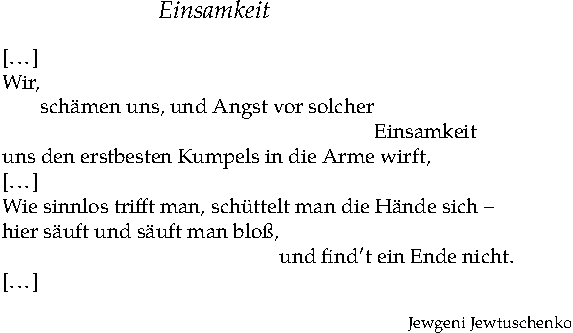
\includegraphics{Roemer-Beispiel3-crop}
\end{center}

Mit der Umgebung \texttt{altverse} können individuell gestaltete Strophen gesetzt werden; sie hat den Effekt, dass z.\,B. bei den paarweise 
strukturierten
Strophen die 2., 4. etc. Zeile um die Länge \verb|\vgap| einrückt.
Als Alternative wird für die \texttt{verse}-Umgebung der Einschluss einzelner
Verse in die \texttt{patverse}-Umgebung angeboten.

\begin{center}
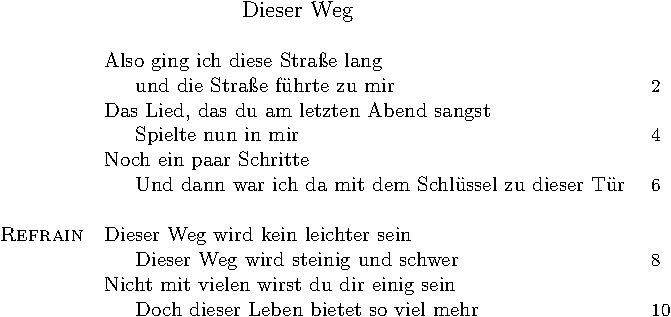
\includegraphics{Roemer-Beispiel-crop}
\end{center}

\begin{lstlisting}
\documentclass[ngerman,a4paper,article]{memoir}
[...]
\settowidth{\versewidth}{Das Lied, das du am letzten Abend sangst}
\PoemTitle*{Dieser Weg}
\begin{verse}[\versewidth]
\linenumberfrequency{2}
\begin{altverse}
  Also ging ich diese Straße lang\\
  und die Straße führte zu mir\\
  Das Lied, das du am letzten Abend sangst\\
  Spielte nun in mir\\
  Noch ein paar Schritte\\
  Und dann war ich da mit dem Schlüssel zu dieser Tür\\!
\end{altverse}

\begin{altverse}
\flagverse{\textsc{Refrain}\quad} Dieser Weg wird kein leichter sein\\
  Dieser Weg wird steinig und schwer\\
  Nicht mit vielen wirst du dir einig sein\\
  Doch dieser Leben bietet so viel mehr\\
\end{altverse}
\linenumberfrequency{0}
\end{verse}
\end{lstlisting}

Das neue poetrytex-Paket von Sam Whited (Juli 2012) ist primär für das Setzen
von poetischen Anthologien geschaffen worden. Die verse-Umgebung wurde darin
etwas modifiziert und in eine \texttt{poem}-Umgebung umgebaut.


\subsection{Darstellen von Reim, Rhythmus und Metrum}

Klassische Gedichte reimen nach bestimmten Schemata. So nennt man beispielsweise
ein Gedicht aus Vierzeilern Quartett. Wenn sich die ersten und die beiden letzten
Zeilen jeweils beim Aussprechen reimen, wird dies als Paarreim bezeichnet. 
Wenn sich das Ende von Verszeilen reimt, ist dies ein Endreim, den es wieder in
verschiedenen Ausprägungen gibt. Veranschaulicht wird dies in der Regel mit
Kleinbuchstaben:

\begin{tabular}{cl}
aabb & Paarreim \\
abab & Kreuzreim \\
abba & umarmender Reim \\
\ldots & \ldots \\
\end{tabular}

Rhythmus und Metrum werden auch Versmaß genannt. Die regelmäßige Abfolge von betonten
und unbetonten Silben ist der Rhythmus, der in der lyrischen Sprache nach einem sich 
wiederholenden Takt (Metrum) aufgebaut sein kann. Eine metrisch gebundene Verszeile 
umfasst mehrere Takte und wird damit als zwei-, drei- oder vierhebig bezeichnet. Man
unterscheidet traditionell nach den Metren verschiedene Rhythmen in den Wortsilben:
den Jambus (unbetont, betont) et cetera. Um mehr Übersichtlichkeit bei der Vermittlung und
Bestimmung des Versmaßes zu bekommen wird die Abfolge von Hebungen und Senkungen auch
graphisch dargestellt. Das übliche Modell nimmt dafür den Backslash (\verb|\|) für eine 
Hebung und "`ein kleines breites U"' ($\cup$) für die Senkung \cite[S.\,17]{Neuhaus}.

Beispielsweise wurde der Daktylus, der schon in der griechischen Ilias Verwendung fand,
während der Klassikepoche in der deutschen Verslehre als Abfolge einer 
betonten und zweier unbetonten Silben definiert.

\begin{tabular}{ll}
betont - unbetont - unbetont: &  \verb|\| $\cup$ $\cup$ \\
\end{tabular}

\begin{lstlisting}
 \verb|\| $\cup$ $\cup$ 
\end{lstlisting}

Um sich die Arbeit etwas zu erleichtern, ist es sinnvoll, Befehle zu definieren.
Es dürfen dafür aber keine Befehle genommen werden, die es schon gibt:
\begin{lstlisting}
\usepackage{xspace}

\newcommand\He{\textbackslash\xspace}%  Hebung
\newcommand\Se{$\cup$\xspace}%  Senkung 
\end{lstlisting}

Der Daktylus tritt in dem folgenden Beispiel auf:

\poemtitle{\textbf{Wür}de der \textbf{Frau}en}
\settowidth{\versewidth}{Ehret die Frauen! sie flechten und weben}
 \poemlines{1} 
\begin{verse}[\versewidth]
\textbf{Eh}ret die \textbf{Frau}en! sie \textbf{flech}ten und \textbf{we}ben\\
\textbf{Himm}lische \textbf{Ro}sen ins \textbf{ir}dische \textbf{Le}ben,\\
\textbf{Flech}ten der \textbf{Lie}be be\textbf{glüc}kendes \textbf{Band},\\
\textbf{Und} in der \textbf{Gra}zie \textbf{züch}tigem \textbf{Schlei}er\\
\textbf{Näh}ren sie \textbf{wach}sam das \textbf{e}wige \textbf{Feu}er\\
\textbf{Schö}ner Ge\textbf{füh}le mit \textbf{hei}liger \textbf{Hand}.\\
\end{verse}
\attrib{Friedrich Schiller}

Das Schema dazu:

\begin{center}

\begin{tabular}{@{}clc@{}}
Vers & Metrum & Reim \\ 
\hline 
  & \He\Se \Se \He\Se \\
1 & \He\Se \Se  \He\Se \Se \He\Se \Se \He\Se  & a\\
2 & \He\Se\Se \He\Se \Se \He\Se\Se \He\Se  & a\\
3 & \He\Se \Se \He\Se \Se\He\Se\Se \He & b\\
4 & \He \Se \Se \He\Se \He\Se\Se \He\Se & c\\
5 & \He\Se \Se \He\Se \Se \He\Se\Se \He\Se & c\\
6 & \He\Se \Se\He\Se \Se \He\Se\Se \He & b\\
\end{tabular}

\end{center}

\begin{lstlisting}
\begin{tabular}{@{}clc@{}}
Vers & Metrum & Reim \\ 
\hline 
 & \He\Se \Se \He\Se \\
1 & \He\Se \Se  \He\Se \Se \He\Se \Se \He\Se  & a\\
2 & \He\Se\Se \He\Se \Se \He\Se\Se \He\Se  & a\\
3 & \He\Se \Se \He\Se \Se\He\Se\Se \He & b\\
4 & \He \Se \Se \He\Se \He\Se\Se \He\Se & c\\
5 & \He\Se \Se \He\Se \Se \He\Se\Se \He\Se & d\\
6 & \He\Se \Se\He\Se \Se \He\Se\Se \He & d\\
\end{tabular}
\end{lstlisting}


Wie zu sehen ist, unterscheiden sich die Verse bei der Betonung der letzten 
Silbe; ist die letzte Silbe im Vers betont, liegt eine männliche, ist sie unbetont
eine weibliche Kadenz
vor. Der Titel, Vers 1, 2, 4, 5 haben weibliche und Vers 3 und 6 haben 
männliche Kadenz.

Wenn man sehen will, wie sich die Hebungen und Senkungen auf die
einzelnen Wörter verteilen, kann der Wortzwischenraum beispielsweise
durch einen Unterstrich markiert werden. Damit keine uneinheitlichen Abstände 
um den Unterstrich entstehen, kann man ein Makro für
den Wortzwischenraum (\verb|Zr|) verwenden:

\verb|\newcommand*{\Zr}{\unskip\textunderscore}|

Würde der Frauen: \He\Se\Zr\Se\Zr\He\Se =\verb|\He\Se\Zr\Se\Zr\He\Se|

%\He\Se\_\Se\_\He\Se \quad = \verb|\He\Se\_\Se\_\He\Se| 


Es ist auch möglich komplexe "`Bausteine"' zu definieren. Beispielsweise
\verb|\daktylus|: \daktylus{} (Daktylus) oder \verb|\anapaest| (Anapäst) 
\anapaest.

\begin{lstlisting}
\newcommand\daktylus{$\textbackslash\cup\cup$\xspace} 
\newcommand\anapaest{$\cup\cup\textbackslash$\xspace} 
\end{lstlisting}

\small
\begin{thebibliography}{1000}
\bibitem
{Neuhaus} Stefan Neuhaus:
\textsl{Grundriss der Literaturwissenschaft}. 
A. Francke Verlag: Tübingen und Basel, 3. überarbeitete und erweiterte Auf\/lage, 
2009.

\bibitem
{Svoboda} Atze Svoboda:
\textsl{Was gesagt werden muss}.
In: Eulenspiegel, Heft 5/2012, S.\,14.

\bibitem
{Willberg} Hans Peter Willberg /Friedrich Forsman:
\textsl{Lesetypografie.}
Verlag Hermann Schmidt: Mainz 2010.

\bibitem
{wilson} Peter R. Wilson/Lars Madsen:
\textsl{The Memoir Class for Configurable Typesetting. User Guide.}
The Herries Press, Normandy Park, WA 2011.
\url{macros/latex/contrib/memoir/memman.pdf}.

\bibitem
{Wilson} Peter R. Wilson:
\textsl{Typesetting simple verse with \LaTeX }. 2004.
\url{macros/latex/contrib/verse/verse.pdf}
\end{thebibliography}

%\end{document}



%\end{document}



\section{Dramen}
\autor{Thomas H. Meyer}

\paket{covington}
\paket{dramatist}
\footcite[xxx]{lesetypografie}




%% lfgw: 2.21 Linguistische Beispiele

%% !TEX root = lfgw.tex

\RequirePackage{iftex}
\RequireLuaTeX
\RequirePackage{luatex85}

\documentclass[%
   ibycus,polutonikogreek,english,french,latin,ngerman,%global definiert!
   %%%draft=false,%
   fontsize=11pt,%
   paper=17cm:24cm,%
   DIV=13,%
   listof=totoc,%
   bibliography=totoc,%
   pagesize%
   ]{scrbook}

\KOMAoption{bibliography}{leveldown}

\usepackage{yfonts}
\usepackage{textgreek}
\usepackage{cjhebrew}[2017/03/06]
\usepackage{amsmath,amssymb} % für forrest
%%%\usepackage{textcomp}
\usepackage{unicode-math}
\usepackage{fontspec}
\defaultfontfeatures{Ligatures=TeX,Scale=MatchLowercase}
%\newfontfamily\GFSDidot{GFS Didot}
\newcommand\gkk[1]{%{\GFSDidot
#1}

\usepackage[]{babel}
%\usepackage[ngerman,noftligs]{selnolig}
%%%\setmainfont{Libertinus Serif} %reicht auch, unten evtl. besser wegen SB
\setmainfont{libertinusserif}[
   Extension = {.otf},
   UprightFont = {*-regular}, ItalicFont = {*-italic},
   BoldFont = {*-bold}, BoldItalicFont = {*-bolditalic},%
   FontFace = {sb}{\updefault}{*-semibold},%
   FontFace = {sb}{it}{*-semibolditalic}]%
\setsansfont{Libertinus Sans}
\setmonofont[Scale=MatchLowercase,FakeStretch=0.85]{DejaVu Sans}%das wird für Griechisch in Codebeispielen gebraucht
\setmathfont{Libertinus Math}
\makeatletter
\newcommand*\sustyle{\addfontfeatures{VerticalPosition=Superior}}
\DeclareTextFontCommand{\textsu}{\sustyle}
\def\@makefnmark{\hbox{\sustyle\@thefnmark}}
\makeatother
\DeclareTextCommandDefault{\textborn}{{\char"002A}}
\DeclareTextCommandDefault{\textdied}{{\char"2020}}
\usepackage[% microtype
   final,%
   tracking=smallcaps,%
   expansion=alltext,%
   protrusion=true%
   ]{microtype}%
\SetTracking{encoding=*,shape=sc}{50}%
\UseMicrotypeSet[protrusion]{basicmath} % disable protrusion for tt fonts

\usepackage[headsepline]{scrlayer-scrpage}
\clearscrheadfoot
\ihead{\headmark}
\ohead{\pagemark}
\pagestyle{scrheadings}

\usepackage[autostyle]{csquotes}
\usepackage[newcommands]{ragged2e}

\usepackage{graphicx}
\graphicspath{{bilder/}}

\usepackage{grffile}
\usepackage[a4,center,cross]{crop}

\usepackage{listings}
\lstdefinestyle{listinglfgw}{%
  inputencoding=utf8,
  extendedchars=true,
  language=[LaTeX]{TeX},
  numbers=left, 
  %stepnumber=3,
  numbersep=5pt, 
  numberfirstline=false,  
  numberstyle=\tiny\textsf,
  basicstyle=\ttfamily\footnotesize,
  keywordstyle=\bfseries,%
  texcsstyle=*\ttfamily\footnotesize\bfseries,%
  %frame=tlrb,
  breaklines=true,
  breakatwhitespace=true,
  breakindent=5pt,
  %postbreak=\mbox{$\hookrightarrow$},
  escapeinside={*@}{@*},
  %showstringspace=false, 
  captionpos=b,
  upquote=true,
  %%%classoffset=0,
  morekeywords={%
  %a
  addbibresource,addplot,Afootnote,alteSeite,autocite,autopar,answerline,alertblock,
  %b
  beginnumbering,Bfootnote,biblerefformat,biblerefmap,biblerefstyle,bonuspointpoints,bibleref,block,
  %c
  Cfootnote,chapter,chbpword,chpword,chpgword,chqword,chsword,chtword,citeauthor,cites,citetitle,columnrulewidth,Columns,columnsposition, center,
  chronology,columns,
  %d
  draw,dictum,deffootnote,deffootnote,description,
  %e
  edtext,endnumbering,enquote,enumi,example,exampleblock,
  %f
  firstlinenum,firstlinenumR,firstpageheadrule,footcite,footcites,footfullcite,fullcite,fillwithgrid,fillwithlines,fillwithdottedlines,Forest,Forest*,
  footnotemargin,fillwithlines, fillwithgrid,
  %h
  hpword,hqword,hsword,htword,hypertarget,hyperlink,hideallsubsection,
  %i
  includegraphics,includeonlyframes,ibibleref,invisible,
  %l
  Lcolwidth,ledsidenote,lemma,linenumincrement,linenumincrementR,
  %m
  msdata,mode,maketitle,multifootsep,
  %n
  newfontface,newfontfamily,node,
  %o
  only,onslide,
  %p
  Pages,parencite,parencites,part,pend,pibibleverse,pbibleverse,pointpoints,printbibheading,printbibliography,printindex,pstart,pgfimage,pgfusepath,
  pgfplothandlerlineto,pgfplotsset,pgfplotxyfile,pbibleref,pibibleref,pgf-pie,plain,
  %q
  quell,question,quote,quotaion,
  %r
  Rcolwidth,reledmac,
  %s
 selectlanguage,setlength,setmainfont,setmonofont,setmsdatalabel,setromanfont,setsansfont,smartcite,smartcites,solutiontitle,setbeamerfont,setbeamercovered,subsection,subsection*,subsubsection,subtitle,solution,solutionorgrid,
  %t
  text,textborn,textcite,textcites,textdelta,textDelta,textdied,texteuro,textgamma,textGamma,textmarried,textsubscript,thealteSeite,tableofcontents,th,TH,
  textalpha, textbeta, textgamma, textdelta, textepsilon, textzeta, texteta, texttheta, textiota, textkappa, textlambda, textmu, textnu,
  textxi, textomikron, textpi, textrho, textsigma, texttau, textupsilon, textphi, textchi,  textpsi, textomega,
  textAlpha, textBeta, textGamma, textDelta, textEpsilon, textZeta, textEta, textTheta, textIota, textKappa, textLambda, textMu, textNu,
  textXi, textOmikron, textPi, textRho, textSigma, textTau, textUpsilon, textPhi, textChi,  textPsi, textOmega, twocolumn,
  %u
  usetheme,usecolortheme,usebackgroundtemplate,useforestlibrary,usepackage,usetikzlibrary,
  %v
  vari,verse,
  %x
  Xafternumber,Xarrangement,Xlemmaseparator,Xinplaceoflemmaseparator,Xinplaceofnumber,Xnonbreakableafternumber,Xnotenumfont,Xnumberonlyfirstinline,Xnumberonlyfirstintwolines,Xsymlinenum,Xtwolines,Xtwolinesbutnotmore,Xtxtbeforenotes
  },   
  literate=
  {á}{{\'a}}1 {é}{{\'e}}1 {í}{{\'i}}1 {ó}{{\'o}}1 {ú}{{\'u}}1
  {Á}{{\'A}}1 {É}{{\'E}}1 {Í}{{\'I}}1 {Ó}{{\'O}}1 {Ú}{{\'U}}1
  {à}{{\`a}}1 {è}{{\`e}}1 {ì}{{\`i}}1 {ò}{{\`o}}1 {ù}{{\`u}}1
  {À}{{\`A}}1 {È}{{\'E}}1 {Ì}{{\`I}}1 {Ò}{{\`O}}1 {Ù}{{\`U}}1
  {ä}{{\"a}}1 {ë}{{\"e}}1 {ï}{{\"i}}1 {ö}{{\"o}}1 {ü}{{\"u}}1
  {Ä}{{\"A}}1 {Ë}{{\"E}}1 {Ï}{{\"I}}1 {Ö}{{\"O}}1 {Ü}{{\"U}}1
  {â}{{\^a}}1 {ê}{{\^e}}1 {î}{{\^i}}1 {ô}{{\^o}}1 {û}{{\^u}}1
  {Â}{{\^A}}1 {Ê}{{\^E}}1 {Î}{{\^I}}1 {Ô}{{\^O}}1 {Û}{{\^U}}1
  {œ}{{\oe}}1 {Œ}{{\OE}}1 {æ}{{\ae}}1 {Æ}{{\AE}}1 {ß}{{\ss}}1
  {ç}{{\c c}}1 {Ç}{{\c C}}1 {ø}{{\o}}1 {å}{{\r a}}1 {Å}{{\r A}}1
  {€}{{\EUR}}1 {£}{{\pounds}}1
}
\lstset{style=listinglfgw}
  
\usepackage[% tcolorbox
  skins,%
  listings,%
  breakable,%
]{tcolorbox}
\tcbset{%
lfgwstyle/.style={%
    before skip=\baselineskip,
    boxrule=0pt,
    %bottomrule=2pt,
    %toprule=2pt,
    %colframe=black,
    colback=black!5,
    coltitle=white,
    bicolor,
    sharp corners,
    colbacklower=white,
    fonttitle=\sffamily\bfseries,
    breakable,
    %label=#1,
}}


\newtcblisting[auto counter,number within=chapter]{lfgwexample}[1]{%
    lfgwstyle,
    fontupper=\small\ttfamily,
    sidebyside,
    listing and text,
    title={Beispiel \thetcbcounter},
    listing options={style=listinglfgw},
    #1,
%text and listing,
}

\newtcblisting[use counter from=lfgwexample,number within=chapter]{lfgwcode}[1]{%
    lfgwstyle,
    fontupper=\small\ttfamily,
    listing only,
    title={Beispiel \thetcbcounter},
    listing options={style=listinglfgw},
    #1,
}

\newtcblisting[use counter from=lfgwexample,number within=chapter]{lfgwprint}[1]{%
    fontupper=\small,
    lfgwstyle,
    text only,
    title={Beispiel \thetcbcounter},
    listing options={style=listinglfgw},
    #1,
}


\usepackage{showexpl}
%\lstset{explpreset={escapeinside={*@}{@*}}}

\usepackage[pagewise]{lineno}
\usepackage{sidenotes}
\usepackage{multicol}
% Für den Abschnitt über Konstituentenanylyse von C. Römer:
\usepackage[linguistics]{forest}
\forestapplylibrarydefaults{linguistics,edges}
\useforestlibrary{edges}
\makeatletter
\let\pgfmathModX=\pgfmathMod@
\usepackage{pgfplots}%
\pgfplotsset{compat=1.14}
\let\pgfmathMod@=\pgfmathModX
\makeatother
%http://tex.stackexchange.com/questions/328972/presence-of-pgfplots-package-breaks-forest-environment-%w-folder-option-en/329015

% Pakete im Bereich Kapitel 3 - Diagramme zeichnen
\usepackage{tikz}
\usepackage[all]{genealogytree}
\usepackage{chronology}
\usepackage{pgf-pie}
\usetikzlibrary{pgfplots.dateplot}
\usetikzlibrary{mindmap}

\deffootnote[1.5em]{1.5em}{1.5em}{\makebox[1.5em][l]{{\fontseries{sb}\selectfont\thefootnotemark\ }}}

\usepackage{enumitem}			% for simple list modifications
\setlist{leftmargin=*,before=\setlength{\rightmargin}{\leftmargin}}

%\usepackage{parallel}


%- Für Lyrik-Satz, Christine Römer:
\usepackage{verse}
\newcommand\He{\textbackslash\xspace}
\newcommand\Se{$\cup$\xspace} 
\newcommand*{\Zr}{\unskip\textunderscore}
\newcommand\daktylus{\textbackslash$\cup\cup$\xspace} 
\newcommand\anapaest{$\cup\cup$\textbackslash\xspace}

% ------------
\usepackage{runic}
\usepackage{hieroglf}
\usepackage[normalem]{ulem} %%% MS: Wofür? Unterstreichungen sollten vermieden werden! LCB: kann \xout
%\usepackage{letterspace} %%% MS: Wofür. Besser direkt \textls aus dem Microtypepaket
%% ------------------------------------------------------------------------
%%   This is a stand-alone version that only provides the letterspacing
%%   commands. Do not use this package together with the `microtype' package.
%%   Please refer to section 7 of the `microtype' documentation.
%% ------------------------------------------------------------------------ 
\usepackage[hyphens]{url}
\usepackage{hologo}
\usepackage{philex}
\def\fg{}
\usepackage{siunitx} %Supreme typesetting of units
%\sisetup{%
%    tight-spacing=true, %
%    %math-rm=\mathsf, 
%    %		text-rm=\sffamily,
%    detect-all, %Zahlen werden in der aktuellen Schrift angezeigt
%    detect-family,
%    exponent-to-prefix  	= true,%
%    round-mode          	= places,% 
%    round-precision     	= 2,%
%    group-minimum-digits 	= 4, % Für "Tausenderpunkt" --> 1.234 anstatt 1234
%    group-separator			={.},% für "12.345" statt "12 345"
%    %  scientific-notation = engineering, % Use multiples of 3 as exponent
%    locale					=DE, % Typeset numbers and units the German way
%    range-phrase 			={$\times$},%
%    %		zero-decimal-to-integer,%aus "2.0" wird "2"
%    range-units				=single,  % --> 2 x 2 m, - auskommentieren für 2 m x 2 m
%    %%%---------
%%    unit-color=myred,
%}

\usepackage[german]{keystroke}% Computer-Tastatur-Tasten in Anweisungs-Texte zu setzen (z.B. \Shift, \Ctrl, \Spacebar).

\usepackage{imakeidx}
\indexsetup{level = \subsection*, toclevel = subsection, noclearpage, headers = {\indexname}{\indexname}}
\makeindex[                title = {Allgemeiner Index}]
\makeindex[name = pakete,  title = {Verzeichnis der Paketnamen}]
\usepackage[% biblatex
   style=authoryear,  
%  style=historische-zeitschrift, % das am liebsten - aber der geht (bei mir?) nicht!
%  pageref=true,
	backend=biber
	]{biblatex}
\addbibresource{lfgw-bibliographie.bib}
%%%\defbibheading{bibliography}{\addchap{#1}} %%%Besser bei \addchap bleiben

\usepackage{fancyvrb}
\makeatletter
\usepackage[% reledmac
   series={A,B,C},%nur die Apparate A B C aktivieren
   noend,%keine Endotenapparate
   noeledsec%keine eledsections et al.
   %noledgroup%keine ledgroups -- das muss hier auskommentiert werden, damit die minipages funktionieren!
]{reledmac}%
\@ifpackagelater{reledmac}{2017/03/20}{%
   % Package is new enough
}{%
\PackageError{reledmac}{Es wird reledmac >= 2.18.1 benötigt.}%
}
\makeatother
\usepackage{reledpar}

\usepackage{varioref}
\usepackage{hyperxmp}
\usepackage{hyperref}
\hypersetup{					% setup the hyperref-package options
	pdftitle={LaTeX für Geisteswissenschaftler},	% 	- title (PDF meta)
	pdfsubject={Handbuch},% 	- subject (PDF meta)
	pdfauthor={varia},	% 	- author (PDF meta)
	pdfauthortitle={},
	pdfcopyright={Copyright (c) \the\year\. All rights reserved.},
	pdfhighlight=/N,
	pdfdisplaydoctitle=true,
	pdfdate={\the\year-\the\month-\the\day}
	pdflang={de},
   pdfencoding=unicode,   % Sorgt für korrekte Umlaute in den pdf-Lesezeichen - thm
	pdfcaptionwriter={varia},
	pdfkeywords={{LaTeX}, {Geisteswissenschaften}},
	pdfproducer={LuaLaTeX},
	pdflicenseurl={http://creativecommons.org/licenses/by-nc-nd/4.0/},
	plainpages=false,			% 	- 
   colorlinks   = true, %Colours links instead of ugly boxes
   urlcolor     =  blue!50!black, %Colour for external hyperlinks
   linkcolor    = blue, %Colour of internal links
   citecolor   = green!50!black, %Colour of citations
   linktoc=page,
  	pdfborder={0 0 0},			% 	-
	breaklinks=true,			% 	- allow line break inside links
 %   bookmarks=true,
	bookmarksnumbered=true,		%
	bookmarksopenlevel=2,
	bookmarksopen=true,		%
   bookmarksdepth=3,
   pdfdisplaydoctitle,
	final=true	% = true, nur bei web-Dokument!! (wichtig!!)
}
\usepackage{bookmark}%advanced bookmarks
\usepackage[% cleveref
  sort,
  nameinlink
  ]{cleveref}%nach hyperref laden

\crefname{tcb@cnt@lfgwexample}{Beispiel}{Beispiele}
\addto\captionsngerman{%
    \crefformat{lfgwexample}{#2Beispiel\,#1#3}%
    \crefformat{lfgwcode}{#2Beispiel\,#1#3}%
    \crefformat{lfgwprint}{#2Beispiel\,#1#3}%
}

\setkomafont{pagehead}{\normalcolor\normalfont\small\upshape}
\setkomafont{pagenumber}{\normalcolor\normalfont\normalsize\bfseries}

\renewcommand*{\glqq}{\textquotedblleft}
\renewcommand*{\grqq}{\quotedblbase}

\providecommand*{\reledmac}{\mbox{\Package{reledmac}}\xspace}

\providecommand*{\LaTeXTeX}{\hologo{(La)TeX}}
\providecommand*{\AmSLaTeX}{\hologo{AmSLaTeX}}
\providecommand*{\AmSTeX}{\hologo{AmSTeX}}
\providecommand*{\biber}{\hologo{biber}}
\providecommand*{\BibTeX}{\hologo{BibTeX}}
\providecommand*{\BibTeXacht}{\hologo{BibTeX8}}
\providecommand*{\ConTeXt}{\hologo{ConTeXt}}
\let\context\ConTeXt
\providecommand*{\emTeX}{\hologo{emTeX}}
\providecommand*{\eTeX}{\hologo{eTeX}}
\providecommand*{\ExTeX}{\hologo{ExTeX}}
\providecommand*{\HanTheThanh}{\hologo{HanTheThanh}}
\providecommand*{\iniTeX}{\hologo{iniTeX}}
\providecommand*{\KOMAScript}{\hologo{KOMAScript}}
\providecommand*{\LaTeX}{\hologo{LaTeX}}
\providecommand*{\LaTeXe}{\hologo{LaTeX2e}}
\providecommand*{\LaTeXIII}{\hologo{LaTeX3}}
\providecommand*{\LaTeXML}{\hologo{LaTeXML}}
\providecommand*{\LuaLaTeX}{\hologo{LuaLaTeX}}
\let\lualatex\LuaLaTeX
\providecommand*{\LuaTeX}{\hologo{LuaTeX}}
\let\luatex\LuaTeX
\providecommand*{\LyX}{\hologo{LyX}}
\providecommand*{\METAFONT}{\hologo{METAFONT}}
\let\MF\METAFONT
\providecommand*{\MetaFun}{\hologo{MetaFun}}
\providecommand*{\METAPOST}{\hologo{METAPOST}}
\providecommand*{\MetaPost}{\hologo{MetaPost}}
\let\MP\METAPOST
\providecommand*{\MiKTeX}{\hologo{MiKTeX}}
\providecommand*{\NTS}{\hologo{NTS}}
\providecommand*{\OzMF}{\hologo{OzMF}}
\providecommand*{\OzMP}{\hologo{OzMP}}
\providecommand*{\OzTeX}{\hologo{OzTeX}}
\providecommand*{\OzTtH}{\hologo{OzTth}}
\providecommand*{\PCTeX}{\hologo{PCTeX}}
\providecommand*{\pdfTeX}{\hologo{pdfTeX}}
\let\pdftex\pdfTeX
\providecommand*{\pdfLaTeX}{\hologo{pdfLaTeX}}
\let\pdflatex\pdfLaTeX
\providecommand*{\PiC}{\hologo{PiC}}
\providecommand*{\PiCTeX}{\hologo{PiCTeX}}
\providecommand*{\plainTeX}{\hologo{plainTeX}}
\providecommand*{\SageTeX}{\hologo{SageTeX}}
\providecommand*{\SLiTeX}{\hologo{SLiTeX}}
\providecommand*{\teTeX}{\hologo{teTeX}}
\providecommand*{\TeXivht}{\hologo{TeX4ht}}
\providecommand*{\TTH}{\hologo{TTH}}
\providecommand*{\virTeX}{\hologo{virTeX}}
\providecommand*{\VTeX}{\hologo{VTeX}}
\providecommand*{\XeLaTeX}{\hologo{XeLaTeX}}
\providecommand*{\XeTeX}{\hologo{XeTeX}}
%%
\newcommand\BibTool{\textsc{Bib\hskip-.1em
      T\hskip-.15emo\hskip-.05emo\hskip-.05eml}\xspace}
\providecommand*{\TikZ}{\textsf{Ti\textit{k}Z}}
%\providecommand*{\pgf/tikz}{\textsf{pgf/Ti\textit{k}Z}}
\def\pgf/tikz{\textsf{pgf/Ti\textit{k}Z}}
\providecommand*{\ALEPH}{\ensuremath{\aleph}}

\providecommand\eV{e.V\kern-0.18em\@ifnextchar.{}{.}\kern0.18em}
\providecommand\dante{\mbox{DANTE~\eV}}
\providecommand\Dante{DANTE,
   Deutschsprachige Anwendervereinigung \TeX~\eV}
\providecommand\DTK{Die \TeX\-ni\-sche Ko\-m{\"o}\-die}
\providecommand\PS{Post\-Script}
\providecommand\TUG{\TeX{} Users Group}
\providecommand\TUGboat{\textsl{TUGboat}}
\let\DANTE\dantelogo
\providecommand*{\TeXLive}{\TeX{}Live}

\def\BibLaTeX{Bib\hologo{LaTeX}}
\let\biblatex\BibLaTeX
\providecommand*{\CTAN}{\texttt{CTAN}\xspace}

\providecommand*{\prog}[1]{\texttt{#1}}
\let\Program\prog

\providerobustcmd*{\paket}[2][]{\textsf{#2}\index[pakete]{\if$#1$#2\else#1\fi}}
\let\Package\paket%zwecks kompatibilität mit DTK
\let\Paket\paket
\newcommand*{\opt}[1]{\texttt{#1}}
\newcommand*{\file}[1]{\texttt{#1}}
\newcommand*{\env}[1]{\texttt{#1}}

\makeatletter
\DeclareRobustCommand\cs[1]{\texttt{\bfseries\char`\\#1}}
\DeclareRobustCommand\meta[1]{%
   \ensuremath\langle
   \ifmmode \expandafter \nfss@text \fi
   {%
      \meta@font@select
      \edef\meta@hyphen@restore
      {\hyphenchar\the\font\the\hyphenchar\font}%
      \hyphenchar\font\m@ne
      \language\l@nohyphenation
      #1\/%
      \meta@hyphen@restore
   }\ensuremath\rangle
}
\def\marg{\@ifstar{\@@marg}{\@marg}}
\providecommand\@marg[1]{%
   {\ttfamily\mdseries\char`\{}\meta{#1}{\ttfamily\mdseries\char`\}}}
\providecommand\@@marg[1]{%
   {\ttfamily\mdseries\char`\{}{\mdseries #1}{\ttfamily\mdseries\char`\}}}
\def\oarg{\@ifstar{\@@oarg}{\@oarg}}
\providecommand\@oarg[1]{%
   {\ttfamily\mdseries[}\meta{#1}{\ttfamily\mdseries]}}
\providecommand\@@oarg[1]{%
   {\ttfamily\mdseries[}{#1}{\ttfamily\mdseries]}}
\providecommand\parg[1]{%
   {\ttfamily\mdseries(}\meta{#1}{\ttfamily\mdseries)}}
\def\meta@font@select{\itshape\mdseries}
\makeatother

\tolerance 1414
\hbadness 1414
\emergencystretch 1.5em
\hfuzz 0.3pt
\widowpenalty=10000
\displaywidowpenalty=10000
\clubpenalty=5000
\interfootnotelinepenalty=9999
\brokenpenalty=2000
\vfuzz \hfuzz
%%%\raggedbottom


% Autorkennung:   Wie soll's aussehen?
\providecommand{\autor}[1]{\hfill\textbf{#1}}

\endinput


%\begin{document}

\section{Linguistische Beispiele}
\autor{Christine Römer}

\subsection{Belege einfügen mit \texttt{philex}}
\label{belege} \index{Belege}
\author{Christine Römer}

Die neuerliche Hinwendung der Linguistik zur Empirie hat es mit sich gebracht, dass eigentlich keine Feststellung ohne reale sprachliche Belege
auskommt. Dies geschieht in der Regel durch eingezogene, durchnummerierte Belege, die mit Grammatikalitätsurteilen in Form von festgelegten Abkürzungen (beispielsweise * =ungrammatisch, ? = fraglich) versehen werden können.
Im laufenden Text wird sich dann auf diese Beispiele bezogen. Im Unterschied zu mathematischen Texten steht die Beispielnummer links und nicht rechts.

Mit dem neueren Paket \paket{philex} ist dies einfach zu bewerkstelligen.
Es wird mit \verb|\usepackage[<package options>]{philex}|\footnote{Paketdokumentation: texdoc philex} in die Präambel eingebunden, es lädt dabei automatisch \paket{linguex}, auf dem es aufbaut, sowie \paket{xspace} und \paket{cgloss4e}. Die möglichen Paketoptionen sind \texttt{hyper, draft, oldpunkt}.

Der Befehl für die Basisumgebung ist  \verb|lb{}{}|, er hat also
zwei obligatorische Argumente: Das erste ist für das Label, den Anker und das zweite für den Inhalt (Beispiel~\ref{example:1}):

\begin{lfgwexample}{label={example:1}}
So wurde in der SDZ am 21.02.\,2017 der Neologismus \emph{Bierpreispremse} geprägt (siehe Beispiel \ref{bier}).

\lb{bier}{Die Bierpreisbremse soll im Zuge einer kompletten Neuorganisation der Wiesn-Finanzierung umgesetzt werden .}

und von weiteren Preisbremsen wird geschrieben, bspw. bei Reuters am 11.04.\,2016 von einer \enquote{Arznei-Preisbremse} (siehe \ref{arznei}).

\lb{arznei}{Pharmaindustrie kritisiert Pläne für Arznei-Preisbremse} 

\end{lfgwexample}

An Stelle einer Nummer kann der Zähler auch auf Buchstaben o.\,ä. mit dem Befehl \verb|\bpaformat{1}{(Beleg~}{)}| umgestellt werden
(wie in \ref{example:2}):

\begin{lfgwexample}{label={example:2}}
\bpaformat{1}{(Beleg~}{)}
\lbpa{kno}{Mietpreisbremse}
\lbpa{hu}{Preisbremse im Grundstückverkauf}
\end{lfgwexample}

Untergliederungen bei den Belegen sind auch möglich (wie in \ref{example:3}/\ref{example:4}):

\begin{lfgwcode}{label={example:3}}
\lbp{clauses}{AdvP}{Adverbiengebrauch:
\lba{first}{Die erste Klasse
\lba{firstnew}{adverbiell: Sie wohnt \emph{hier}.}
\lbb{lastnew}{prädikativ: Sie ist \emph{hier}.}
\lbz{attr}{attributiv: Die \emph{dort} wohnt hier.}}
\lbb{second}{Die zweite Klasse
\lba{adverb}{nur adverbial: Sie liest \emph{gern}.}}}
\end{lfgwcode}

\begin{lfgwprint}{label={example:4}}
\lbp{clauses}{AdvP}{Adverbiengebrauch:
\lba{first}{Die erste Klasse
\lba{firstnew}{adverbiell: Sie wohnt \emph{hier}.}
\lbb{lastnew}{prädikativ: Sie ist \emph{hier}.}
\lbz{attr}{attributiv: Die \emph{dort} wohnt hier.}}
\lbb{second}{Die zweite Klasse
\lba{adverb}{nur adverbial: Sie liest \emph{gern}.}}}
\end{lfgwprint}


Grammatikalitätsurteile mit dem Befehl \verb|\oddity{ }| einfügen (wie in \ref{example:5}/\ref{example:6}):

\begin{lfgwcode}{label={example:5}}
Genitiv-s für Eigennamen?
\lb{gram}{
\lba{grama}{\oddity{*}die Entwicklung Friedrich Schiller}
\lbb{gramb}{\oddity{?}die Entwicklung Friedrich Schiller-s}
\lbc{grama}{\oddity{*}die Entwicklung Friedrich Schiller}
}
\end{lfgwcode}

\begin{lfgwprint}{label={example:6}}
Genitiv-s für Eigennamen:
\lb{gram}{
\lba{grama}{\oddity{*}die Entwicklung Friedrich Schiller}
\lbb{gramb}{\oddity{??}die Entwicklung Friedrich Schiller-s}
\lbz{gramz}{\oddity{}die Entwicklung Friedrich Schiller}
}
\end{lfgwprint}

Auch für Glossierungen kann das Paket eingesetzt werden 
(wie in dem Beispiel \ref{example:7}/\ref{example:6} aus der Paketdokumentation):

\begin{lfgwcode}{label={example:7}}
\lb{gloss}{\gll Wenn jemand in die Wüste zieht ... \\
If someone in the desert draws and lives ... \\
\trans ‘if one retreats to the desert and ... ’}
\end{lfgwcode}

\begin{lfgwprint}{label={example:8}}
\lb{gloss}{\gll Wenn jemand in die Wüste zieht ... \\
If someone in the desert draws and lives ... \\
\trans ‘if one retreats to the desert and ... ’}
\end{lfgwprint}



%\end{document}




\section{Querverweise im Text}
\autor{Thomas Hilarius Meyer}

%Philipp meint: Lukas hatte vorgeschlagen, zumindest /auch/ das cleveref-Paket hier vorzustellen, das nimmt einem etwas Arbeit ab

\lstinline/\label{key}/

\lstinline/\ref{key}/

\lstinline/\pageref{key}/


\section{Eigene Kommandos und Umgebungen definieren}
\label{makros}

\minisec{Kommandos}

\minisec{Umgebungen}

% !TeX root = lfgw.tex
\usepackage[german]{keystroke}% Computer-Tastatur-Tasten in Anweisungs-Texte zu setzen (z.B. \Shift, \Ctrl, \Spacebar
\chapter{Textpassagen in nicht-lateinischen Alphabeten einbetten}

Hinweis von Lukas C. Bossert:
Für einzelne Wörter kann man auch \url{http://www.perseus.tufts.edu/hopper/morph} nutzen.
bzw. für antike Texte auch hieraus (\url{http://www.perseus.tufts.edu/hopper/collection?collection=Perseus:collection:Greco-Roman}) kopieren.

\section{Allgemeines: babel, Unicode}

Grundlegend ist der Artikel von Axel Kielhorn in der DTK.%
\footcite{kielhorn:dtk2014}

\section{Eingabe von Unicode-Sonderzeichen}
\label{unicodeeingabe}

\minisec{Eingabe von Unicode-Zeichen in
einem \Program{Emacs} Buffer}
\label{unicodeviaemacs}

\section{Test Block von arktisvogel}

\minisec{Wie arktisvogel die \texttt {lfgw}-Makros anwendet}
\label{cpftestalpha}

Es befriedigt \LaTeX{}-Benutzer die Programme \LuaLaTeX ,
\METAFONT , \pdfLaTeX und \XeLaTeX{} zu benutzen. Um einen
Kropfnugn zu gestalten, benutzen sie einen Paket wie
\Package{booktabs} oder \paket{graphicx}.
Nach einige \cs {biegen\marg {Buenos Aires}} in der
\cs {biegen\oarg {Sao Paulo}} zu bestimmen. Auch zwei
\cs {biegen\parg {Ciudad Mexico}} Sachen sind
\meta {skateboard} wichtig.

\minisec{Wie arktisvogel die \texttt {Keystroke}-Paket anwendet}
\label{cpftestbety}

Das Paket \paket{keystroke} bietet die Möglichkeit,
Tastendrücke darzustellen.

\minisec{Almut A.\ Altquist}

\textit{Achtung: zur Zeit die Benutzung der keystroke Paket
liefert nur französiche Tasten-Darstellungen!}\/ Das
Paket \paket{keystroke} bietet die Möglichkeit,
Tastendrücke darzustellen. Für ja,
die \hbox{\keystroke{J}-Taste} ist gut. Wenn sie \Del{} und %
\Ins{}%
und %
\Esc{}%
und %
\Shift{}%
und %
\Ctrl{}%
und %
\Home{}%
und %
\End{}%
und %
\PgUp{}%
und %
\PgDown{}%
und %
\PrtScroll{}%
und %
\Spacebar{}%
und %
\Break{} sehen wollen, geht es in Ordnung.

\minisec{Bertha B.\ Bertzbach}
Der Schriftsteller Markus Arktisvogel braucht die Symbole %
\Esc{}%
und %
\Shift{}%
und %
\Ctrl{}%
und %
\Alt{}%
und %
\Return{}%
und %
\Spacebar{}%
um alle Probleme zu lösen.

Karl hat drei \Spacebar{}%
und %
\Return{}%
und %
\BSpace{}%
und %
\Tab{}%
und %
\Alt{}%
und %
\AltGr{}%
und %
\NumLock{}%
und %
\UArrow{}%
und %
\DArrow{}%
und %
\LArrow{}%
und %
\RArrow{} vorhanden.

$$\diamondsuit\qquad\diamondsuit\qquad\diamondsuit$$

Zwei Methoden ermöglichen die Eingabe von
Unicode-Zeichen in \Program{Emacs}:

\minisec{Methode 1:\enspace Hexdezimalzahl eingeben}
\Program{Emacs}-Dokumentation benutzt die Schreibweise: %
\texttt{C-x 8}
um den Vorgang zu beschreiben: man druckt die Tastenkombination
\Ctrl$+$\keystroke{X}%
\space%
\keystroke{8}.

In diesem Fall heisst das: %
\Ctrl$+$\keystroke{X}%
\space%
\keystroke{8}%
\Return{}%
\meta{Unicode Codepoint}%
\Return . ermöglicht die direkte Eingabe einer Unicode
Zeichen.

Um einem \enquote{Capitulum} einzugeben: %
\hbox{\Ctrl$+$\keystroke{X}}%
\keystroke{8}%
\Return{}%
\keystroke{2}%
\keystroke{E}%
\keystroke{3}%
\keystroke{F}%
\space%
\Return{}%

% Die Unicode Codepoint 2021 ist: Double Dagger, und sieht so aus: ``‡''
% Die Unicode Codepoint 2045 ist: Left Square Bracket With Quill, und sieht so aus: ``⁅''
% Die Unicode Codepoint 2046 ist: Right Square Bracket With Quill, und sieht so aus: ``⁆''
% Die Unicode Codepoint 2e3f ist: Capitulum, und sieht so aus: ``⸿''
% Die Unicode Codepoint 02ad ist: Latin Letter Bidental Percussive, und sieht so aus: ``ʭ''
% Die Unicode Codepoint 169b ist: Ogham Feather Mark, und sieht so aus: ``᚛''
% Die Unicode Codepoint 169c ist: Ogham Reversed Feather Mark, und sieht so aus: ``᚜''
%
\minisec{Methode 2:\enspace \Program{Emacs}-Aliase Benutzen}

\Program{Emacs} hat eine lange Liste vorgefertigte Aliase%
\footnote{Ein \enquote{Alias} ist eine Aufruf, mit der
mehrere Funktionen, durch einen neuen Befehl ersetzt werden kann.
Es wird benutzt, um Zeit zu sparen und weniger zu tippen.}%
um oft benutzte Unicode Zeichen einzugeben. Zuerst, mit nur
drei Tastendrücke: um eine \enquote{no-break space} einzugeben: %
\hbox{\Ctrl$+$\keystroke{X}}%
\keystroke{8}%
\Spacebar .

Einige Aliase sind fertig nach drei Tastendrücke. Andere
benötige vier Tastendrücke. Ich möchte das Wort \enquote{Français}
eingeben. Mit %
\hbox{\Ctrl$+$\keystroke{X}}%
\keystroke{,}%
\keystroke{C}%
\space%
kann ich einen \enquote{c} mit eine Cedille eingeben.

Ich möchte das Wort \enquote{mañana} eingeben. Mit %
\hbox{\Ctrl$+$\keystroke{X}}%
\keystroke{\char126}%
\keystroke{N}%
\space%
kann ich einen \enquote{n} mit einen Tilde eingeben.

Es gibt auch Aliase für drei verschiedene Bruchzahlen. Aber
\TeX{}-Benutzer haben nie Probleme damit gehabt, Bruchzahlen
zu setzen.

\minisec{Eingabe von Unicode-Zeichen in \Program{gedit}}
\label{unicodeviagedit}

\Program{gedit} ermöglicht auch die direket Eingabe einer Unicode
Zeichen durch Tastendruck-Folge %
\hbox{\Shift$+$\Ctrl$+$\keystroke{U}}%
\meta{Unicode Codepoint}%
\Return{}%
\space%
ermöglicht die direkte Eingabe einer Unicode
Zeichen.

Mit %
\hbox{\Shift$+$\Ctrl$+$\keystroke{U}}%
\keystroke{2}%
\keystroke{0}%
\keystroke{2}%
\keystroke{2}%
\Return{}%
\space%
kann ich einen \enquote{Bullet} eingeben.

%% \minisec{Eingabe von Unicode-Zeichen in \Program{nano}}
%% \label{unicodevianano}

%% \Program{GNU nano} ermöglicht auch die direket Eingabe einer
%% Unicode Zeichen.

%% \begin{foreigndisplayquote}{english}
%% Entering Text

%% nano is a “modeless” editor. This means that all keystrokes, with the exception of Control and Meta sequences, enter text into the file being edited.

%% Characters not present on the keyboard can be entered in two ways:

%% For characters with a single-byte code, pressing the Esc key twice and then typing a three-digit decimal number (from 000 to 255) will enter the character with the corresponding value.

%% For any possible character, pressing M-V (Alt+V) and then typing a six-digit hexadecimal number (starting with 0 or 1) will enter the character with the corresponding Unicode value.
%% \end{foreigndisplayquote}
%%
%% \textbf{Texteingabe}

%% \Program{nano} erlaubt die Eingabe jede mögliche Zeichen
%% (ausser Meta-Sequenzen und Steuerung-Sequenzen) direkt in
%% einem Textdatei einzugeben.

%% Es gibt eine Methode um Zeichen die in dem Bereich 0$_{10}$
%% bis zum 255$_{10}$ (hex FF$_{16}$)~-- ein Byte Zeichen~--
%% einzugeben. Ein zweite Methode erlaubt die Eingabe von zwei
%% Byte Zeichen.

%% Methode 1:~zweimal die %
%% \Esc\Esc{}$\langle$\texttt {dreistellige Dezimalzahl}$\rangle$

%% Methode 2:~\Alt$+$\keystroke{V}$\langle$\texttt {sechsstellige Hexadezimalzahl}$\rangle$%

\minisec{Eingabe direkt mit der Tastatur}

Lohnend besonders bei den modernen Fremdsprachen: Anschaffen einer Tastatur in der jeweiligen
Sprache.

Problem im altphilologischen Bereich: Akzente und (bei Hebräisch) Vokalzeichen sind heute
nicht mehr verwendet und fehlen deshalb auf den heutigen Tastaturen.

\minisec{Auswahl über Maus-gestützte tools}
KCharselect

\begin{figure}
 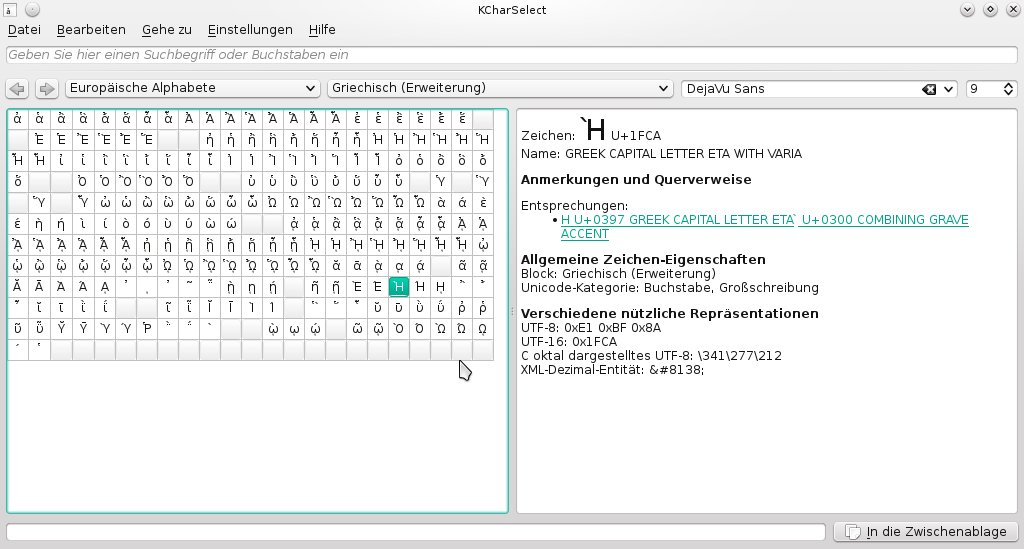
\includegraphics[width=\textwidth]{kcharselect}
 \caption{Mit dem KDE-Programm KCharselect kann man Unicode-Buchstaben immerhin mit der Maus
 auswählen.}
\end{figure}

\minisec{Eingabe über die Zeichennummer}

Vgl.\ Abschnitt \ref{utf8codes} auf Seite \pageref{utf8codes}.

\section{Griechisch}
\index{Griechisch}

Es gibt (mindestens...) drei verschiedene Möglichkeiten, griechische Textpassagen einzubinden;
je nach Aufgabenbreich sind diese verschieden gut geeignet:


\minisec{Möglichkeit I: Einzelbuchstaben}

Die erste Möglichkeit besteht in der Eingabe m.\,H. der Einzelnbuchstaben-Symbole des Paketes
\paket{textgreek}; das Verfahren ist in Abscnitt \ref{griechEinzelbuchstaben}, 
S.~\pageref{griechEinzelbuchstaben}, beschrieben.

Dieses Verfahren eignet sich eigentlich nur für ganz kurze Einsprengsel im Umfang von 
einzelnen Zeichen bis maximal ca.\ einem Wort.


\minisec{Möglichkeit II: Transkription mit \paket{ibycus}}

Die zweite Methode eignet sich demgegenüber hervorragend, wenn es darum geht auch etwas 
längere (alt-)griechische Passagen in ein ansonsten deutschsprachiges Dokument~-- m.\,H. eines
deutschen Computers mit QWERTZ-Tastatur~-- einzugeben.

Dabei wird für die griechischen Buchstaben eine Art Transkription in lateinischen Buchstaben
vorgenommen, die sich bei etwas Übung sehr leicht benutzen lässt.

Das Paket \paket{ibycus}%
\footnote{Paketdokumentation: texdoc ibycus-babel}
definiert dabei eine Art Pseudosprache für \paket{babel},
in der Dokumenpräambel ist also anzugeben:

\begin{lstlisting}
 \usepackage[ibycus,ngerman]{babel}
\end{lstlisting}

Im Dokument stehen dann eine Umgebung \lstinline/ibycus/ sowie ein Befehl \lstinline/\ibygr{}/
zur Verfügung:


Das wird zu:

 \begin{ibycus}
  (Hrodo'tou Qouri’ou i(stori’hs a)po’decis h(’de,
  ...
  h(‘n ai)ti’hn e)pole’mhsan a)llh’loisi. 
  \end{ibycus}

  Und jetzt ein einzelnes griechisches Wort~-- \ibygr{a)rxai=a gra’mmata}~-- im Text.





\minisec{Möglichkeit III: Direkteingabe von Unicode-Text}

Die dritte Möglichkeit besteht darin, die griechischen Schriftzeichen direkt als Unicode-Zeichen
in das \LaTeX -Dokument einzufügen. Dazu reicht es aus, dem Paket \paket{babel} die 
(alt-)griechische Sprache als zusätzliche Option anzugeben: 
\lstinline/\usepackage[polutonikogreek,ngerman]{babel}/.
\footnote{Achtung! Bei den meisten \LaTeX -Installationen im Rahmen von Linux-Distributionen muss
man Pakete nachinstallieren!}
Damit \LaTeX{} den griechischen Font richtig ansprechen kann, braucht auch das Paket \paket{fontenc} 
eine Modifikation: \lstinline/\usepackage[OT1,T1]{fontenc}/.

Dann kann mit \lstinline/\selectlanguage{polutonikogreek}/ auf Griechisch umgeschaltet werden.

Der folgende Bibelvers wurde aus dem Internet unverändert in das \LaTeX -Dokument
kopiert. Derzeit werden nicht alle Zeichen in meinem KDE-Editor (kile) korrekt dargestellt (vgl. Abb.);
dennoch gibt \LaTeX{} alle Zeichen richtig wider:

\begin{figure}
 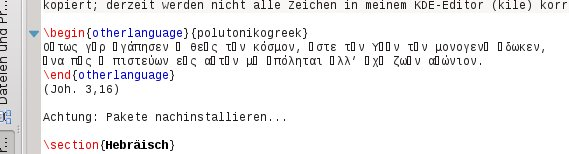
\includegraphics[width=\textwidth]{ersatzdarstellung}
 \caption{KDE kann nicht alle aus dem Internet kopierten Unicode-Zeichen korrekt darstellen;
 Buchstaben mit Akzent und Spiritus bekommen eine (nichtssagende) Ersatzdarstellung!}
\end{figure}


\begin{otherlanguage}{polutonikogreek}
Οὕτως γὰρ ἠγάπησεν ὁ Θεὸς τὸν κόσμον, ὥστε τὸν Υἱὸν τὸν μονογενῆ ἔδωκεν, 
ἵνα πᾶς ὁ πιστεύων εἰς αὐτὸν μὴ ἀπόληται ἀλλ’ ἔχῃ ζωὴν αἰώνιον.
\end{otherlanguage}
(Joh. 3,16)

Diese Methode dürfte sich in der Praxis am ehesten eignen, wenn bereits ein Textcorpus
(z.\,B. via Internet) ediert und Unicode-Erfasst vorliegt, und Textpartien ins eigene Dokument
ohne Veränderungen übernommen werden sollen~-- so wie z.\,B. bei Zitaten aus der Bibel oder
der klassischen Literatur.

Will man selbst (alt-)griechische Textpassagen schreiben, scheint das Ibykus-Verfahren
wesentlich angenehmer und effizienter.


\section{Hebräisch}
\index{Hebräisch}

Das Paket \paket{cjhebrew} von Christian Justen eignet sich hervorragend für 
Theologen und Orientalisten, denn es erlaubt auch die Vokalisierung sowie die Verwendung 
von Akzenten. Auch das Problem der rechts- bzw. linksläufigen Schriften wird sehr
Anwenderfreundlich~-- im Sinne von Anwendern an einem westlichen PC mit ansonsten 
lateinischen Alphabet~-- gelöst:

Nach \lstinline/\usepackage{cjhebrew}/%
\footnote{Eine besondere Angabe z.\,B. bei \paket{babel} ist nicht nötig.}
steht v.\,a. der Befehl \lstinline/\cjRL{}/ 
-- für hebräische Einzelworte im laufenden Absatz~-- sowie die 
Umgebung \lstinline/cjhebrew/ 
-- für ganze Absätze in Hebräisch~-- zur Verfügung.

Beide drehen die Folge der Schriftzeichen automatisch um, so dass hebräische Textpartien
ganz gewohnt eingegeben werden können. Dabei sind für die einzelnen Zeichen sehr leicht 
merkbare Codes definiert worden:

Der Beginn des biblischen Buches Genesis~-- \enquote{Im Anfang schuf Gott Himmel und Erde...} --
wird so eingegeben:

\begin{lstlisting}
\begin{cjhebrew}
 b*e:re'+siyt b*ArA' 'E:lohim 'et ha+s*amayim w:'et hA'ArE.s;
\end{cjhebrew} 
\end{lstlisting}

Mit etwas Eingewöhnung arbeitet man mit diesem System \emph{wesentlich} schneller und 
angenehmer, als wenn man etwa die Unicode-Zeichen mit Hilfe eines grafischen Auswahlwerkzeuges
einzeln auswählt...

Die Bearbeitung mit \LaTeX{} ergibt:

\begin{cjhebrew}
 b*e:re'+siyt b*ArA' 'E:lohim 'et ha+s*amayim w:'et hA'ArE.s;
\end{cjhebrew}

Wegen der Einzelheiten der Zeichen-, Vokal-, Akzent- und Satzzeichen-Codierung (inkl. z.\,B. 
Mem finalis) sei auf die Paketdokumentation verwiesen.

\section{Russisch}
\index{Kyrillisch}
\index{Russisch}

\section{Koptisch}
\index{Koptisch}

\section{Altkirchenslawisch}
\index{Altkirchenslawisch}

\paket{churchslavonic}


\section{Arabisch}
\index{Arabisch}

Ist \paket{arabtex} noch aktuell?

\section{Hieroglyphen}
\index{Hieroglyphen}
\index{Ägyptologie}

\paket{hieroglf}~-- \enquote{The Poor Man’s Hieroglyphic Font}


 \pmglyph{K:l-i-o-p-a-d:r-a} 
 

\section{Keilschrift}
\index{Keilschrift}

\paket{archaic} und andere...

\section{Runen}
\index{Runen}

Das Paket \paket{runic} von Peter Wilson stellt die Runen des sog.\ Futhark-Alphabets bereit.
Nach \lstinline/\usepackage{runic}/ gibt es den Befehl \lstinline/\textfut{}/, der 
die Runen ausgibt. Dies ist die Transkription:

\begin{center}
\begin{tabular}{ll}
 \lstinline/F/ &	\textfut{F} \\
 \lstinline/U/ &	\textfut{U} \\
 \lstinline/\Fthorn/ &	\textfut{\Fthorn} \\
 \lstinline/A/ &	\textfut{A} \\
 \lstinline/R/ &	\textfut{R} \\
 \lstinline/K/ &	\textfut{K} \\
 \lstinline/G/ &	\textfut{G} \\
 \lstinline/W/ &	\textfut{W} \\
 \lstinline/H/ &	\textfut{H} \\
 \lstinline/N/ &	\textfut{N} \\
 \lstinline/I/ &	\textfut{I} \\
 \lstinline/J/ &	\textfut{J} \\
 \lstinline/Y/ &	\textfut{Y} \\
 \lstinline/P/ &	\textfut{P} \\
 \lstinline/X/ &	\textfut{X} \\
 \lstinline/S/ &	\textfut{S} \\
 \lstinline/T/ &	\textfut{T} \\
 \lstinline/B/ &	\textfut{B} \\
 \lstinline/E/ &	\textfut{E} \\
 \lstinline/M/ &	\textfut{M} \\
 \lstinline/L/ &	\textfut{L} \\
 \lstinline/\Fng/ &	\textfut{\Fng} \\
 \lstinline/D/ &	\textfut{D} \\
 \lstinline/O/ &	\textfut{O} \\
 \lstinline/:/ &	\textfut{:} \\
 \end{tabular}
 \end{center}


\section{Phonetische Alphabete}


\section{Kurzschriften}
\index{Kurzschrift}
\index{Schnellschrift}

\minisec{Tironische Noten}
\index{Tironische Noten}


\minisec{Deutsche Einheits-Kurzschrift}
DEK\footcite{sarman:dtk2009/1}
\index{Deutsche Einheits-Kurzschrift}
\index{DEK}


\minisec{Pitman-Kurzschrift}
\index{Pitman}

% !TeX root = lfgw.tex
%\chapter{Texte parallel setzen}

\newcommand\reledpar{\mbox{\Package{reledpar}}\xspace}

\section{Vertikal parallelisierte Texte}
\autor{Philipp Pilhofer}

\DefineShortVerb{\+}

\noindent Es gibt mehrere \LaTeX-Pakete, mit denen man Texte spalten- oder seitenweise parallel setzen kann, d.h., dass die entsprechenden Paragraphen in der linken und der rechten Spalte bzw. auf der linken und der rechten Seite immer auf der jeweils gleichen Höhe beginnen.
Hier wird das Paket \reledpar vorgestellt, weil es gut funktioniert, viele Möglichkeiten bietet und auch aktuell noch gewartet wird.
Dieses Paket arbeitet eng mit dem im vorangegangenen Kapitel vorgestellten \reledmac-Paket zusammen; daher werden einige der hier besprochenen Befehle und Einstellungen in der \reledmac-Dokumentation erklärt.

Um Texte vertikal zu parallelisieren, ist nicht viel zu tun. Ich gehe hier erst auf die spaltenweise Parallelisierung ein, danach komme ich zur seitenweisen Parallelisierung. Zuerst muß das Paket geladen werden: +\usepackage{reledpar}+.


\subsection{Spaltenweise parallelisierte Texte}

Wie schon für \reledmac gezeigt,%
\footnote{Im folgenden beziehe ich mich öfters auf den Abschnitt zu den \reledmac-Grundlagen, \cref{apparate-grundlagen-anfang}, \cpagerefrange{apparate-grundlagen-anfang}{apparate-grundlagen-ende}.}
muß der Text für die linken und rechten Spalten jeweils mit +\beginnumbering+ und +\endnumbering+ eingefasst werden.%

Der Einfachheit halber lassen wir hier die Paragraphen-Einteilung durch +\autopar+ erledigen;
die Paragraphen werden dann automatisch erkannt und jeweils auf derselben Höhe begonnen.
Damit dies auch funktioniert, müssen vor und nach den Paragraphen Leerzeilen stehen.

Die Textabschnitte für die linke Spalte müssen nun noch in eine +Leftside+-Umgebung eingefügt werden, analog die rechte Spalte in eine +Rightside+-Umgebung.
Diese beiden Umgebungen selbst müssen von einer +pairs+-Umgebung (man beachte die jeweilige Groß-/Kleinschreibung) umfaßt werden.

Die Spalten werden nun mit +\Columns+ ausgegeben. Hier ein Beispiel:


%das hier steht hier nur, um die im vorigen Kapitel vorgenommenen Einstellungen zurückzunehmen
\firstlinenum{5}
\linenumincrement{5}

\begin{lfgwcode}{}
\begin{pairs}
\begin{Leftside}
\beginnumbering
\autopar
\selectlanguage{latin}

Gallia est omnis divisa in partes tres, 
    quarum unam incolunt Belgae,
    aliam Aquitani,
    tertiam, qui ipsorum lingua Celtae, nostra Galli appellantur.

Hi omnes lingua institutis legibus inter se differunt.

\endnumbering
\end{Leftside}

\begin{Rightside}
\beginnumbering
\autopar

Gallien als ganzes ist in drei Teile gegliedert,
    deren erster die Belger bewohnen,
    den zweiten die Aquitanier,
    den dritten jene, die in ihrer eigenen Sprache Kelten, in der unseren Gallier genannt werden.

Sie alle unterscheiden sich hinsichtlich der Sprache, 
    der (staatlichen) Einrichtungen und der Gesetze von einander.
    
\endnumbering
\end{Rightside}
\end{pairs}

\Columns
\end{lfgwcode}

Dieser Code wird so ausgegeben:

%damit die columns in die bsp-box passen:
\columnsposition{C}
\setlength{\Lcolwidth}{0.425\textwidth}
\setlength{\Rcolwidth}{0.425\textwidth}

\begin{lfgwprint}{}
\begin{pairs}
\begin{Leftside}
\beginnumbering
\autopar
\selectlanguage{latin}

Gallia est omnis divisa in partes tres, 
    quarum unam incolunt Belgae,
    aliam Aquitani,
    tertiam, qui ipsorum lingua Celtae, nostra Galli appellantur.

Hi omnes lingua institutis legibus inter se differunt.

\endnumbering
\end{Leftside}

\begin{Rightside}
\beginnumbering
%\pstart
\autopar

Gallien als ganzes ist in drei Teile gegliedert,
    deren erster die Belger bewohnen,
    den zweiten die Aquitanier,
    den dritten jene, die in ihrer eigenen Sprache Kelten, in der unseren Gallier genannt werden.

Sie alle unterscheiden sich hinsichtlich der Sprache, 
    der (staatlichen) Einrichtungen und der Gesetze von einander.
    
\endnumbering
\end{Rightside}
\end{pairs}

\Columns
\end{lfgwprint}

Analog zu den oben für \reledmac vorgestellten Optionen gibt es nun für die rechten Spalten entsprechende Befehle.
Für die Zeilenzähler sind dies beispielsweise +\firstlinenumR{<num>}+ und +\linenumincrementR{<num>}+.
Hinzu kommen die für Spaltensatz erwartbaren Möglichkeiten:
Mit der Länge +\columnrulewidth+ kann man einen Trennungsstrich einführen, mit +\Lcolwidth+ und +\Rcolwidth+ die Spaltenbreite verändern.
Mit dem Befehl +\columnsposition{<pos>}+ läßt sich die Orientierung der Spalten ändern: Standardmäßig orientieren sie sich am rechten Rand, mit +Ĺ+ orientieren sie sich am linken Rand, mit +C+ sind sie zentriert.
Alle Längen müssen mit +\setlength{<name>}{<laenge>}+ angepaßt werden, hier ein Beispiel für die vorgestellten Befehle: 

\begin{lfgwcode}{}
\firstlinenumR{2}
\linenumincrementR{2}
\setlength{\columnrulewidth}{0.5pt}
\setlength{\Lcolwidth}{0.425\textwidth}
\setlength{\Rcolwidth}{0.425\textwidth}
\columnsposition{C}
\end{lfgwcode}

Bemerkenswert ist vielleicht noch die Paket-Option +movecolumnspositiononrightpage+ für Bücher:
Ist diese gesetzt, werden die \enquote{rechten} Spalten auf rechten Seiten links gesetzt, d.h. die \enquote{rechten} Spalten stehen immer auf der Innenseite.
Weitere Optionen bietet das \reledpar-Handbuch.


\subsection{Seitenweise parallelisierte Texte}

Nach der Lektüre des vorangegangenen Abschnittes ist es sehr einfach, Texte seitenweise zu parallelisieren, was sich vor allem bei Editionen mit Übersetzung anbietet:
So kann auf den linken Seiten der Originaltext gedruckt werden, auf der rechten Seite die Übersetzung; die einzelnen Paragraphen stehen, wie im spaltenweise parallelisierten Satz, auf derselben Höhe.

Die Texte müssen, wie im Spaltensatz, in +\beginnumbering+/+\endnumbering+ und +\autopar+ sowie die +Leftside+-/+Rightside+-Umgebung eingefaßt werden.
Anders sind hier nur die Namen der äußeren Umgebung, die heißt statt +pairs+ in diesem Fall +pages+, und der Befehl, um alles auszugeben, lautet statt +\Columns+ nun +\Pages+.



%%\begin{lfgwprint}
%\begin{pages}
%\begin{Leftside}
%\beginnumbering
%der Text für die linken Spalten/Seiten
%\endnumbering
%\end{Leftside}
%
%\begin{Rightside}
%\beginnumbering
%der Text für die rechten Spalten/Seiten
%\endnumbering
%\end{Rightside}
%\end{pages}
%
%\Pages
%%\end{lfgwprint}
\UndefineShortVerb{\+}

%%%das war früher einmal:
%Das Paket \paket{parallel} von Matthias Eckermann stellt eine Umgebung 
%\lstinline/Parallel/ zur Verfügung, in der mit den Befehlen 
%\lstinline/\ParallelLText{...}/ und 
%\lstinline/\ParallelRText{...}/ die jeweils links- bzw. rechtsstehenden Texte
%angegeben werden können.
%
%Durch den Befehl \lstinline/\ParallelPar/ wird ein neuer \enquote{Doppelabsatz} begonnen.
%
%\begin{lstlisting}
% \linenumbers
% \begin{Parallel}{.45\textwidth}{.45\textwidth}
%  \ParallelLText{Gallia est omnis divisa in partes tres ...}
%  \ParallelRText{Gallien als ganzes ist in drei Teile...}
%  \ParallelPar
%  \ParallelLText{Hi omnes...}
%  \ParallelRText{Sie alle...}
% \end{Parallel}
%\end{lstlisting}
%
%Beim Erzeugen der \lstinline/Parallel/-Umgebung ist für die linke und rechte Seite ihre
%jeweilige Breite anzugeben; das kann als absolute Angabe (in mm oder cm) oder als 
%Bezugnahme zu einem Wert wie \lstinline/\textwidth/ (der Breite des aktuellen 
%Satzspiegels) erfolgen.
%
%Das obige Beispiel erzeugt folgende Ausgabe:
%\bigskip 
%
%\linenumbers
%\begin{Parallel}{.45\textwidth}{.45\textwidth}
%  \ParallelLText{Gallia est omnis divisa in partes tres, 
%    quarum unam incolunt Belgae,
%    aliam Aquitani,
%    tertiam, qui ipsorum lingua Celtae, nostra Galli appellantur.}
%  \ParallelRText{Gallien als ganzes ist in drei Teile gegliedert,
%    deren erster die Belger bewohnen,
%    den zweiten die Aquitanier,
%    den dritten jene, die in ihrer eigenen Sprache Kelten, in der unseren Gallier genannt werden.}
%  \ParallelPar
%  \ParallelLText{Hi omnes lingua institutis legibus inter se differunt.}
%  \ParallelRText{Sie alle unterscheiden sich hinsichtlich der Sprache, 
%    der (staatlichen) Einrichtungen und der Gesetze von einander.}
% \end{Parallel}
%\nolinenumbers
%
%(Zu der Zeilennummerierung vgl. Abschnitt \ref{zeilennummer} auf S.~\pageref{zeilennummer}.)
%
%\minisec{Das Paket \paket{paracol}}
%
%\paket{paracol}
% !TEX root = lfgw.tex

\chapter[Mehrere Apparate setzen: Erstellen einer kritischen Edition]{Mehrere Apparate setzen:\\Erstellen einer kritischen Edition\footnote{Dieses Kapitel bildet eine aktualisierte Fassung meines Artikels \cite{pilhofer:dtk2017}.}}

%\dictum[?]{Kritik ist überall, zumal in Deutschland, nötig.}

\autor{Philipp Pilhofer}

\index{Apparat} \index{Varianten}%TODO %das geht noch more sophisticated
\index{reledmac|(}

\label{reledmac}

%\enquote{Edieren ist eine Erziehung zur Bescheidenheit [...] Es ist ferner eine Erziehung zur 
%Genauigkeit, wie alle Philologie.}%
%\footnote{Erich Trunz, Ein Tag aus Goethes Leben. Acht Studien zu Leben und Werk, München 1999, S.~213.}

\newcommand\vari[3][]{%
\edtext{#2}{%
  \if$#1$\lemma{\gkk{#2}}\else\lemma{\gkk{#1}}\fi
  \Cfootnote{#3}}}

\newcommand\quell[3][]{%
\edtext{#2}{%
  \if$#1$\lemma{\gkk{#2}}\else\lemma{\gkk{#1}}\fi
  \Bfootnote{#3}}}

\newsavebox\bspbox
\newenvironment{reledmacbsp}[1]{%
  \begin{lrbox}{\bspbox}
  \begin{minipage}[t]{0.95\linewidth}
  \beginnumbering
  #1%
  \pstart[\subsubsection*{Strabons Geographika XIV 5,1}]%
}%
{%
  \pend
  \endnumbering
  \end{minipage}%
  \end{lrbox}%
  \colorbox{black!5}{%
  \begin{minipage}{.985\textwidth}%
  \usebox\bspbox
  \end{minipage}}
  \medskip
}

\newcommand\bsplineenum{\firstlinenum{2}\linenumincrement{2}}

\newcounter{alteSeite}
\setcounter{alteSeite}{269}
\newcommand\alteSeite{{|\ledsidenote{\quad\emph{T}~\thealteSeite}}}%stepcounter machen wir hier nicht, sonst zählt er ja immer weiter ...

\VerbatimFootnotes
\DefineShortVerb{\+}

\section{Zur Geschichte des Problems}

In diesem Kapitel stelle ich einen Weg vor, mit \LaTeX\ eine wissenschaftlich-kritische Edition eines Textes zu setzen. Eine solche Edition stellt hohe Anforderungen an das Satzprogramm: weil mehrere voneinander unabhängige kritische Apparate unterstützt werden müssen. Diese können verschiedene Aufgaben haben, im vorgestellten Beispiel sind dies:

\begin{enumerate}\label{pil:apparat}
\item Der Zeugen-Apparat: Dieser zeigt zeilengenau an, auf Basis welcher Handschriften die entsprechenden Bereiche des Textes erstellt wurden.

\item Der Quellen-Apparat: In diesem Apparat wird auf Parallelstellen in anderen Texten verwiesen, die dem Autor/der Autorin 
möglicherweise als Vorlage dienten, oder auf die er/sie anspielt.

\item Der textkritische Apparat: Dieser ist das Kernstück der kritischen Edition. Hier werden Text-Varianten der einzelnen Handschriften angezeigt, die von dem oben gedruckten Text 
abweichen. 
Dabei wird die Zeile und das 
Wort (oder die Wörter) aus dem Haupttext (das »Lemma«) angegeben, dahinter die 
abweichenden Varianten mit den jeweiligen Handschriften.
\end{enumerate}

In Zeiten des Bleisatzes wurden einfach so viele Korrekturdurchgänge absolviert, 
bis das satztechnische Ergebnis zufriedenstellend war. In den Zeiten des beginnenden 
Computersatzes wurde die Lage unübersichtlicher, es gibt Berichte der 
Benutzung von Microsoft Word unter 
Zuhilfenahme von Schere und Kleber.~\cite[34]{stockhausen:mde2016/2} Heute wird meistens 
ein Word-ähnliches Programm namens \Program{Classical Text Editor (CTE)} verwendet, 
das die verschiedenen Apparate in vielen kleinen Fenstern organisiert. 
Der \Program{CTE} erfüllt also die technischen Grundbedingungen, dennoch liegen die 
Nachteile auf der Hand: Die entstehenden Dateien liegen in einem binären Format 
vor und können nur mit dem \Program{CTE} bearbeitet werden. 
Man ist also für alle Zeiten auf einen lauffähigen \Program{CTE} angewiesen, 
die Entwicklung des proprietären Codes hängt jedoch seit 20 Jahren an einer einzigen Person.
Eine spätere Weiterverarbeitung der druckfertigen Edition ist aus den binären Dateien 
fast nicht möglich; für eine digitale Edition beispielsweise müsste man wieder ganz von vorne beginnen.
In Zeiten schmaler werdender Budgets sind auch die Lizenzkosten nicht zu vernachlässigen.

Bei der Nutzung von \LaTeX{} stellen sich diese Probleme nicht, Darüber hinaus bieten sich 
weitere Vorteile wie der überlegene Textsatz. Mit \Package{ednotes} und \reledmac 
liegen zwei Pakete vor, die allen Anforderungen einer kritischen Edition gerecht 
werden.\footnote{Auf das Paket \Package{ednotes} von Uwe Lück gehe ich 
hier nicht weiter ein, ein ausführlicher \TUGboat-Artikel liegt diesem Paket bei. 
Eine Arbeit, die mit diesem Paket erstellt wurde, ist~\cite{mariev:joh_ant}.} 
\reledmac befindet sich seit Ende der 80er Jahren in mehr oder weniger steter Fortentwicklung. 
Der aktuelle Maintainer Maïeul Rouquette arbeitet Fehlerberichte oder Feature-Wünsche 
freundlich und effizient ab.%
\footnote{%
	Das Paket \reledmac geht 
	ursprünglich auf das \plainTeX{}-Paket \Package[reledmac]{edmac} von John Lavagnino und 
	Dominik Wujastyk zurück. Dieses wurde ab 2003 von Peter Wilson für \LaTeX{} 
	als \Package[reledmac]{ledmac} portiert und weiterentwickelt. Im Jahr 2011 hat Maïeul 
	Rouquette das Paket übernommen und erst als \Package[reledmac]{eledmac}, später als \reledmac fortgeführt. 
	Als Beispiel für die Effizienz mag hier erwähnt sein, dass ein Fehler im Paket 
	\reledmac, der beim Schreiben dieser Zeilen aufgefallen ist, ganze zwölf Minuten nach 
	Absenden des Bug-Reports gefixt war.
	Da \reledmac häufig mit Fehlerkorrekturen verbessert wird, lohnt es sich, das Paket auf dem aktuellsten Stand zu halten.}
Das Paket hat sich in mehreren publizierten 
Editions(groß)projekten als gleichermaßen stabil und flexibel erwiesen. %\footnote{
Beispielsweise verwendet die Erlanger Athanasius"=Arbeitsstelle %verwendet 
seit zehn Jahren 
\Package[reledmac]{(re)ledmac} und hat damit bereits mehrere Bände publiziert, unter anderem%beispielsweise 
~\cite{athanasius_3_1_4}. Zu den technischen und insbesondere \TeX{}nischen 
Hintergründen vgl.~\cite{stockhausen:mde2016/2}. Eine unvollständige Liste der Editionen in den unterschiedlichsten 
Sprachen, die auf \Package[reledmac]{(rel)edmac} basieren, findet sich unter~\cite{reledmac-benutzung}. 
\reledmac ist 
ausführlich dokumentiert, die verschiedenen Funktionen werden auf 70 Seiten 
erläutert; zudem liegen dem Paket 40 Beispieldateien bei, die viele der 
Konfigurationsmöglichkeiten vorführen.\footnote{Neben der Dokumentation des Paketes selbst beschäftigt sich weitere Literatur mit den Funktionen von \Package{reledmac}: \cite{reledmac-literatur}.}


\section{Die Grundlagen}\label{apparate-grundlagen-anfang}

Auf den folgenden Seiten will ich nicht alle dieser Funktionen vorstellen, sondern nur eine kurze Einführung geben und eine mögliche Grundkonfiguration für eine den Anforderungen entsprechende kritische Edition vorstellen. 
Davon ausgehend sollte es dann einfach sein, eventuelle Sonderwünsche mit Hilfe der Dokumentation umzusetzen.

Das Paket wird mit +\usepackage[<opt>]{reledmac}+ geladen. Da \reledmac ein sehr mächtiges Paket ist, kann es den \TeX-Durchlauf spürbar verlangsamen. Je nach Anforderungsszenario und verwendeter Hardware kann es sinnvoll sein, die nicht benötigten Funktionen des Paketes abzuschalten. Standardmäßig ermöglicht \reledmac je fünf Endnoten-, »kritische« Fußnoten- und »normale« Fußnoten-Apparate 
(jeweils mit A bis E bezeichnet). Es lassen sich auch weitere Apparate hinzufügen. Mit »normalen« Fußnoten bezeichne ich die üblichen Fußnoten, die oben im Text eine Zahl setzen 
und unten hinter der Zahl den Text der Fußnote. Bei einer »kritischen« Fußnote findet sich keine Markierung im Text, dafür wird 
unten eine Zeilenangabe gemacht und das Lemma wiederholt, bevor der Text der Fußnote folgt. In unserem Beispiel gehe ich nur auf die Fußnoten-Apparate ein, und wie oben erwähnt, brauchen wir nur drei dieser Apparate, der Rest 
(inklusive einiger weiterer hier nicht besprochener Möglichkeiten) wird also abgeschaltet:

\begin{lfgwcode}{}
\usepackage[%
  series={A,B,C},% nur die Apparate A B C aktivieren
  noend,         % keine Endnotenapparate
  noeledsec,     % keine eledsections et al.
  noledgroup     % keine ledgroups
]{reledmac}
\end{lfgwcode}

Der Text der Edition muss zwingend von +\beginnumbering+ \dots{} +\endnumbering+ 
eingefasst werden. Jeder Paragraph muss mit +\pstart+ begonnen und mit +\pend+ beendet 
werden. Alternativ kann dies mit +\autopar+ vereinfacht werden.~\cite[17]{reledmac-benutzung} 
Die Paragraphen-Nummer kann man automatisch ausgeben lassen, wenn man dies 
möchte.\footnote{Dafür gibt es die Befehle +\numberpstarttrue+ und +\sidepstartnumtrue+. 
  Der erste fügt zu Beginn des Paragraphen die Nummer ein, der zweite schreibt die Nummer an 
den Rand und schaltet den sichtbaren Zeilenzähler ab.} 
Hier ein Beispiel der bisher eingeführten Befehle:\footnote{Der Beispieltext ist Strabons Geographika XIV 5,1. 
Text und Übersetzung folgen dabei mit Abweichungen der Radtschen Ausgabe (\cite[96\psq]{radt:strabon4}). 
Die hier verwendeten Text-Varianten, Handschriftenzeugen und Quellen-Belege sind rein 
fiktiv und nur gewählt, um die Funktionsweise des Paketes \reledmac einfach zu veranschaulichen.}

\begin{lfgwcode}{}
\beginnumbering
\pstart[\subsubsection{Strabons Geographika XIV 5,1}]
§\null§Τῆς§~§Κιλικίας§~§δὲ§~§τῆς§~§ἔξω§~§τοῦ§~§Ταύρου§~§ἡ§~§μὲν§~§λέγεται§~§τραχεῖα§~§ἡ§~§δὲ§~§πεδιάς;
§\null§τραχεῖα§~§μέν,§~§ἧς§~§ἡ§~§παραλία§~§στενή§~§ἐστι§~§καὶ§~§οὐδὲν§~§ἢ§~§σπανίως§~§ἔχει§~§\dots{}
\pend
\endnumbering
\end{lfgwcode}

Das Ergebnis sähe bisher folgendermaßen aus:

\bigskip\bigskip%warum sich die Abstände hier anders verhalten ...?

\noindent
\begin{reledmacbsp}{}
\gkk{Τῆς Κιλικίας δὲ τῆς ἔξω τοῦ Ταύρου ἡ μὲν λέγεται τραχεῖα ἡ δὲ πεδιάς;
τραχεῖα μέν, ἧς ἡ παραλία στενή ἐστι καὶ οὐδὲν ἢ σπανίως ἔχει \dots{}}
\end{reledmacbsp}

Die Zeilen zwischen den +numbering+-Befehlen werden fortlaufend gezählt. Schon bei der Zeilenzählung gibt es viele Einstellungsmöglichkeiten. 
Mit dem Befehl +\lineation{<arg>}+ lässt sich erreichen, dass der Zeilenzähler auf jeder Seite (+page+) oder mit jedem Paragraphen 
(+pstart+) zurückgesetzt wird. Normalerweise wird der Stand des Zeilenzählers in jeder fünften Zeile angezeigt. 
Dies lässt sich mit +\linenumincrement{<num>}+ ändern: Um die Funktionalität auf möglichst wenig 
Raum erklären zu können, wollen wir hier mit +\linenumincrement{2}+ den Zählerstand in 
jeder zweiten Zeile anzeigen lassen. Mit +\firstlinenum{2}+ wird eingestellt, dass der Zeilenzähler in der 2. Zeile auch zum ersten Mal steht.

Für Zwischenüberschriften, die keine Zeilennummern (und also auch keinen Apparat) erhalten sollen, kann man die üblichen Befehle verwenden: 
+\chapter+, +\section+ usw. Zu beachten ist dabei, dass diese als optionales Argument des +\pstart+"=Befehles 
mitgegeben werden müssen. Möglich sind auch Überschriften mit Zeilenzählung und Apparat, dazu sind die Befehle +\eledchapter+, +\eledsection+, usw. zu verwenden 
(diese können innerhalb eines Paragraphen ohne Beschränkungen verwendet werden).\footnote{Da wir diese Art von Überschriften im vorliegenden Beispiel nicht brauchen, haben wir sie in der Präambel mit +noeledsec+ abgeschaltet.}

Neben dem Text sind Randbemerkungen durch verschiedene Befehle möglich, beispielsweise über +\ledsidenote{<anm>}+. 
Diese Randbemerkungen lassen sich etwa dazu verwenden, den Seitenumbruch einer älteren Edition desselben Textes anzuzeigen. Dazu definiert man am besten einen Befehl, der einerseits an der richtigen Stelle der Zeile ein entsprechendes Zeichen 
(hier: +|+) setzt und gleichzeitig am Rand die neue Seite ausgibt.
Durch einen eingebauten Zähler wird die ausgegebene Seitenzahl bei jeder Benutzung automatisch um eins erhöht.
Dieses Beispiel gibt am Rand den Buchstaben \emph{T} (der für die alte Edition steht) mit der Seitenzahl 269 aus:

\begin{lfgwcode}{}
\newcounter{alteSeite}
\setcounter{alteSeite}{269}
\newcommand\alteSeite{{|\ledsidenote{\emph{T}~\thealteSeite\stepcounter{alteSeite}}}}
\end{lfgwcode}

Mit den nun neu eingeführten Befehlen sieht der Beispielcode so aus:

\begin{lfgwcode}{}
\firstlinenum{2}% ab der zweiten Zeile die Nummern anzeigen
\linenumincrement{2}% ... und zwar jede zweite Zeile
\beginnumbering
\pstart[\subsubsection{Strabons Geographika XIV 5,1}]
§\null§Τῆς§~§Κιλικίας§~§δὲ§~§τῆς§~§ἔξω§~§τοῦ§~§Ταύρου§~§ἡ§~§μὲν§~§λέγεται§~§τραχεῖα§~§ἡ§~§δὲ§~§πεδιάς;
§\null§τραχεῖα§~§μέν,§~§ἧς§~§ἡ§~§παραλία§~§\alteSeite{}§~§στενή§~§ἐστι§~§καὶ§~§οὐδὲν§~§ἢ§~§σπανίως§~§ἔχει§~§\dots{}
\pend
\endnumbering
\end{lfgwcode}

Das Ergebnis hat sich damit auch verändert und sähe nun folgendermaßen aus:

\noindent
\begin{reledmacbsp}{\bsplineenum}
\gkk{Τῆς Κιλικίας δὲ τῆς ἔξω τοῦ Ταύρου ἡ μὲν λέγεται τραχεῖα ἡ δὲ πεδιάς;
τραχεῖα μέν, ἧς ἡ παραλία \alteSeite{} στενή ἐστι καὶ οὐδὲν ἢ σπανίως ἔχει \dots{}}
\end{reledmacbsp}

\label{apparate-grundlagen-ende}


\section{Die Apparate}

Ich hatte oben drei Apparate erwähnt, die wir für unser Beispiel verwenden wollen: 
Zeugen-Apparat, Quellen-Apparat und textkritischer Apparat (siehe Seite~\pageref{pil:apparat}). 
Die letzten beiden haben eine ähnliche Funktionsweise: 
Ein Wort (oder einige Wörter) aus dem Text, das Lemma, soll unten im Apparat mit Zeilenangabe wiedergegeben werden, dahinter folgt eine Art von Kommentar oder Anmerkung 
zum Lemma. Der erstgenannte Apparat hingegen soll zeilenweise angeben, 
bei welchen Handschriften (den »Zeugen«) die jeweiligen Zeilen nachgewiesen werden können.


\subsection{Quellen- und textkritischer Apparat}

Ich gehe zuerst auf den Quellen-Apparat und den textkritischen Apparat ein. Diese Apparate lassen sich 
mit dem Befehl +\edtext{<lemma>}{<befehl>}+ ansprechen. +lemma+ ist dabei das Wort (oder die Wörter), 
zu dem im Apparat eine Anmerkung gemacht werden soll:\footnote{In dem Fall, dass ein Wort mehrfach 
innerhalb einer Zeile vorkommt, ist der Befehl +\sameword{<lemma>}+ anzuwenden. Es ist zu beachten, dass 
der unten eingeführte Befehl +\vari+ auf den Befehl +\lemma+ zurückgreift: Dieser Tatsache muss 
bei der Benutzung von +\sameword+ Rechnung getragen werden. Näheres ist der Dokumentation von 
\reledmac zu entnehmen.} Das +lemma+ wird einmal normal oben im Text ausgegeben und einmal im Apparat mit Zeilenangabe. Bei +befehl+ ist einzutragen, 
in welchen Apparat die Anmerkung mit 
dem +lemma+ aufgenommen werden soll, 
dazu existieren die Befehle +\Afootnote{<anm>}+, +\Bfootnote{<anm>}+ usw. Für den textkritischen Apparat, der ganz unten stehen soll, wählen wir Apparat C. Eine textkritische Bemerkung zum Wort \gkk{Κιλικίας} sähe also so aus, wenn die Handschrift V dort \gkk{Πισιδίας} liest 
(es ist zu beachten, dass \reledmac bis zu drei \LaTeX"=Durchläufe braucht, bis die Zeilennummern im Apparat richtig sind):

\begin{lfgwcode}{}
§\null§Τῆς§~§\edtext{§\null§Κιλικίας}{\Afootnote{§\null§Πισιδίας§~§V}}§~§δὲ§~§τῆς§~§ἔξω§~§τοῦ§~§Ταύρου§~§\dots{}
\end{lfgwcode}

Wenn das +lemma+ etwas länger ist, kann es sinnvoll sein, es nicht vollständig im Apparat wiederzugeben, sondern es
stattdessen abzukürzen. 
Dafür existiert der Befehl +\lemma{<lemma_kurz>}+, der auch im +befehl+-Feld von +\edtext+ zu verwenden ist.
Die Verwendung ist auch dann sinnvoll, wenn der Text des Lemmas andere Befehle enthält, die unten im Apparat nicht noch einmal wiederholt werden sollen, wie +\alteSeite+ oder verschachtelte +\edtext+-Befehle.
Hier ein Anwendungsbeispiel (unten auf Seite~\pageref{Pilhofer-Beispiel-Lemma-kurz} wird dies auch noch anschaulich gemacht):

\begin{lfgwcode}{}
\dots{},§~§ἧς§~§\edtext{§\null§ἡ§~§παραλία§~§\alteSeite{}§~§στενή§~§ἐστι}{\lemma{§\null§ἡ§~§\dots{}
§\null§ἐστι}\Bfootnote{Anmerkungstext}}§~§καὶ§~§οὐδὲν§~§ἢ§~§σπανίως§~§ἔχει§~§\dots{}
\end{lfgwcode}

Da dies schnell etwas unübersichtlich wird, führen wir einen Befehl für Text-Varianten ein, 
nämlich: +\vari[<lemma_kurz>]{<lemma>}{<anm>}+ (die Angabe des abgekürzten Lemmas ist optional). Dieser erledigt alle genannten Aufgaben auf einmal:

\begin{lfgwcode}{}
\newcommand\vari[3][]{%
  \edtext{#2}{\if$#1$#2\else\lemma{#1}\fi
    \Cfootnote{#3}}}
\end{lfgwcode}

Der neue Befehl sieht im Beispieltext dann so aus:

\begin{lfgwcode}{}
§\null§Τῆς§~§\vari{§\null§Κιλικίας}{§\null§Πισιδίας§~§V}§~§δὲ§~§τῆς§~§ἔξω§~§τοῦ§~§Ταύρου§~§\dots{}
\end{lfgwcode}

Der angegebene Code führt nach genügend vielen Durchläufen zu diesem Ergebnis:

\noindent
\begin{reledmacbsp}{\bsplineenum}
\gkk{Τῆς \vari{Κιλικίας}{\gkk{Πισιδίας} V} δὲ τῆς ἔξω τοῦ Ταύρου \dots{}}
\end{reledmacbsp}

Für den Quellen-Apparat wählen wir Apparat B und definieren entsprechend den Befehl +\quell[<lemma_kurz>]{<lemma>}{<anm>}+:

\begin{lfgwcode}{}
\newcommand\quell[3][]{%
  \edtext{#2}{\if$#1$#2\else\lemma{#1}\fi
    \Bfootnote{#3}}}
\end{lfgwcode}

Gehen wir hier einmal davon aus, dass die Wörter \gkk{ἡ παραλία στενή ἐστι} schon bei einem fiktiven 
älteren Autor namens Konon Paraliotes stehen, in seinem ebenso fiktiven Werk \gkk{Κοσμογραφία} VI 7. Dann würde der Beispielcode so aussehen (nun auch unter Verwendung des abgekürzten 
Lemmas und zudem mit einer weiteren Lesart: Handschrift G bietet das \gkk{ἔξω} nicht):

\begin{lfgwcode}{}
§\null§Τῆς§~§\vari{§\null§Κιλικίας}{§\null§Πισιδίας§~§V}§~§δὲ§~§τῆς§~§\vari{§\null§ἔξω}{\emph{del.}§~§G}
§\null§τοῦ§~§Ταύρου§~§ἡ§~§μὲν§~§λέγεται§~§τραχεῖα§~§ἡ§~§δὲ§~§πεδιάς;
§\null§τραχεῖα§~§μέν,§~§ἧς§~§\quell[§\null§ἡ§~§\dots{}§~§ἐστι]{§\null§ἡ§~§παραλία§~§\alteSeite{}§~§στενή§~§ἐστι}%
{Konon§~§Paraliotes,§~§Κοσμογραφία§~§VI§~§7}§~§καὶ§~§οὐδὲν§~§ἢ§~§σπανίως§~§ἔχει§~§\dots{}
\end{lfgwcode}

Mit beiden Apparaten kommen wir zu diesem Zwischenergebnis:

\noindent
\begin{reledmacbsp}{\bsplineenum}
\gkk{Τῆς \vari{Κιλικίας}{\gkk{Πισιδίας} V} δὲ τῆς \vari{ἔξω}{\emph{del.} G} 
τοῦ Ταύρου ἡ μὲν λέγεται τραχεῖα ἡ δὲ πεδιάς;
τραχεῖα μέν, ἧς \quell[\gkk{ἡ \dots{} ἐστι}]{ἡ παραλία \alteSeite{} στενή ἐστι}%
{Konon Paraliotes, \gkk{Κοσμογραφία} VI 7} καὶ οὐδὲν ἢ σπανίως ἔχει \dots{}}
\end{reledmacbsp}


\subsection{Der Zeugen-Apparat}

Jetzt benötigen wir nur noch den Zeugen-Apparat. Dieser funktioniert etwas anders als die beiden bisher beschriebenen 
Apparate. Standardmäßig verwendet \reledmac dafür den Apparat A.\footnote{Dies lässt sich über +\setmsdataseries{<app>}+ ändern.} 
Mit dem Befehl +\msdata{<zeugen>}+ werden die ab dieser Stelle herangezogenen Handschriften angegeben. Diese Angabe ist gültig bis 
zur nächsten Angabe über +\msdata{<zeugen>}+ oder bis zu einem +\stopmsdata+.

Nehmen wir an, unser Text sei in insgesamt vier Handschriften V, U, G und T belegt; 
in V und T sind nur die ersten Zeilen erhalten, in U und G der komplette Text. Dann sähe unser Beispiel so aus:

\begin{lfgwcode}{}
\msdata{G§~§T§~§U§~§V}§\null§Τῆς§~§\vari{§\null§Κιλικίας}{§\null§Πισιδίας§~§V}§~§δὲ§~§τῆς§~§\vari{§\null§ἔξω}{\emph{del.}§~§G}
§\null§τοῦ§~§Ταύρου§~§ἡ§~§μὲν§~§λέγεται§~§τραχεῖα§~§ἡ§~§δὲ§~§πεδιάς;
§\null§τραχεῖα§~§μέν,§~§ἧς§~§\quell[§\null§ἡ§~§\dots{}§~§ἐστι]{§\null§ἡ§~§παραλία§~§\alteSeite{}§~§στενή§~§ἐστι}%
{Konon§~§Paraliotes,§~§Κοσμογραφία§~§VI§~§7}§~§καὶ§~§οὐδὲν
\vari{§\null§ἢ§~§σπανίως}{§\null§ἢ§~§σπανιαίτερον§~§V§~§U;§~§\emph{del.}§~§T}§~§ἔχει§~§τι§~§χωρίον
\msdata{G§~§U}§\null§ἐπίπεδον,§~§καὶ§~§ἔτι§~§ἧς§~§ὑπέρκειται§~§ὁ§~§Ταῦρος§~§οἰκούμενος§~§κακῶς§~§μέχρι§~§καὶ§~§τῶν
§\null§προσβόρρων§~§πλευρῶν§~§τῶν§~§περὶ§~§Ἴσαυρα§~§καὶ§~§τοὺς§~§Ὁμοναδέας§~§μέχρι§~§τῆς§~§Πισιδίας;
\end{lfgwcode}

Noch nicht sonderlich schön, aber immerhin technisch vollständig, sieht der Zwischenstand so aus:

\label{Pilhofer-Beispiel-Lemma-kurz}%
\noindent
\begin{reledmacbsp}{\bsplineenum}
\gkk{\msdata{G T U V}
Τῆς \vari{Κιλικίας}{\gkk{Πισιδίας} V} δὲ τῆς \vari{ἔξω}{\emph{del.} G} 
τοῦ Ταύρου ἡ μὲν λέγεται τραχεῖα ἡ δὲ πεδιάς;
τραχεῖα μέν, ἧς \quell[\gkk{ἡ \dots{} ἐστι}]{ἡ παραλία \alteSeite{} στενή ἐστι}%
{Konon Paraliotes, \gkk{Κοσμογραφία} VI 7} καὶ οὐδὲν 
\vari{ἢ σπανίως}{\gkk{ἢ σπανιαίτερον} V U; \emph{del.} T} ἔχει τι χωρίον\stopmsdata
\msdata{G U}ἐπίπεδον, καὶ ἔτι ἧς ὑπέρκειται ὁ Ταῦρος οἰκούμενος κακῶς μέχρι καὶ τῶν
προσβόρρων πλευρῶν τῶν περὶ Ἴσαυρα καὶ τοὺς Ὁμοναδέας μέχρι τῆς Πισιδίας;\stopmsdata}
\end{reledmacbsp}


\section{Die satztechnischen Feinheiten}

Nun wollen wir noch einige optische Feinheiten anpassen und die Anmerkungen platzsparender organisieren. 
Ich stelle hier einige der Möglichkeiten vor. Es kommen nun zahlreiche verschiedene Befehle vor, 
die aufgrund der vielen Einstellungsmöglichkeiten etwas verwirrend erscheinen mögen. Man sollte 
sich jedoch vor Augen halten, dass man diese Einstellungen nur einmal vornehmen muss, 
und sobald alles nach Wunsch aussieht, 
muss man daran nichts mehr ändern. 
%Der Vorteil ist aber, wenn dann doch noch etwas geändert 
%werden muss, braucht es nur eine einzige Änderung an einem dieser Befehle, und schon ist das ganze Dokument umgestellt.
Muss aber doch noch etwas geändert werden, genügt eine
          einzige Korrektur an einem dieser Befehle, um das ganze
          Dokument umzustellen.

Fast alle der hier vorgestellten Befehle haben ein optionales Argument: Wenn es leer bleibt, gilt der Befehl für alle Apparate; wenn man dort einen oder 
mehrere Apparate mit ihrem Buchstaben angibt, gilt der Befehl nur für diese.
%
Die Anordnung der Anmerkungen im Apparat wird mit dem Makro +\Xarrangement[<app>]{<option>}+ angepasst. 
Ich wähle hier die platzsparende Option +paragraph+, es wären aber auch zwei- oder dreispaltiger Satz der Anmerkungen möglich: +twocol+, +threecol+. Der Befehl muss \emph{vor} dem +\beginnumbering+ stehen. 

\begin{sloppypar}
Im gezeigten Beispiel sind in Z.~1 mehrere Varianten zu besprechen; die Zeilennummer wird 
im Moment einfach wiederholt. Schöner ist es, wenn stattdessen nur ein Trennsymbol 
angezeigt wird. Setzt man +\Xnumberonlyfirstinline[<app>][<bool>]+ auf +true+, ist die doppelte 
Zeilennummer weg. Dann muss auch noch +\Xnumberonlyfirstintwolines[<app>][<bool>]+ auf \texttt{true} 
gesetzt werden, damit bei mehrzeiligen Lemmata auf jeden Fall die Zeilennummern 
angezeigt werden. Mit +\Xsymlinenum{<symbol>}+ kann noch ein Trennsymbol 
definiert werden, in unserem Fall +||+.
%
Um die Übersichtlichkeit der Apparate zu steigern, lassen wir durch den Befehl 
+\Xnotenumfont[<app>]{<stil>}+ die Zeilennummern etwas dicker setzen.
%
Mit +\Xnonbreakableafternumber[<app>]+ verhindern wir, dass im Apparat nach der Angabe der Zeilennummer die Zeile umgebrochen wird.
\end{sloppypar}

Für den Fall, dass ein Lemma über zwei Zeilen geht, soll nicht beispielsweise »2--3« 
ausgegeben werden, sondern »2\,f.«. Dies legen wir mit +\Xtwolines[<app>]{<abk>}+ 
fest. Bei Lemmata, die über drei oder mehr Zeilen gehen, sollen die Zeilennummern 
aber vollständig ausgegeben werden, daher benutzen wir: +\Xtwolinesbutnotmore[<app>]+.

Mit +\Xlemmaseparator[<app>]{<sep>}+ kann eingestellt werden, was direkt hinter dem 
Lemma ausgegeben werden soll, die Standard-Einstellung ist +]+. Für den Quellen-Apparat 
und den textkritischen Apparat soll es stattdessen ein »+:+« sein.

%%der Zeugen-Apparat:
%\setmsdatalabel{}%kein Label-Text ("Ms.") benötigt
%\Xtxtbeforenotes[A]{}%kein Text am Anfang des Apparats
%\Xafternumber[A]{0pt}%kein spatium nach der Zeilennummer
%\Xlemmaseparator[A]{}%kein Lemma-Trenner
%\Xinplaceofnumber[A]{0pt}%kein spatium, wenn die Zeilennummern nicht angezeigt werden (auf Seiten ohne neue msdata)

Dann nehmen wir noch einige Einstellungen für den Sonderfall des Zeugen-Apparates vor. Bisher 
steht hier hinter den Zeilennummern »Ms.«, dann der Lemma\-sepa\-rator und dann die 
Zeugen. Hinter den Zeilennummern sollen aber nur die Zeugen stehen, weiter nichts. 
Mit +\setmsdatalabel{<label>}+ streichen wir das »Ms.« vor jeder Anmerkung; 
allerdings erscheint nun am Anfang des Apparates ein »Ms.« Dieses entfernen 
wir mit dem Befehl +\Xtxtbeforenotes[<app>]{<label>}+. Mit +\Xafternumber[<app>]{<laenge>}+ 
setzen wir das \emph{Spatium} nach der Zeilennummer auf +2pt+, mit dem gerade 
schon verwendeten Befehl +\Xlemmaseparator+ löschen wir den Lemmaseparator. 
Damit statt des Lemmaseparators kein \emph{Spatium} erscheint, setzen wir 
+\Xinplaceoflemmaseparator[<app>]{<laenge>}+ auf +0pt+.

Auf Seiten, die durchgehend durch dieselben Handschriften bezeugt sind, stehen keine Zeilenangaben, sondern nur diese Handschriften. Bei den aktuellen Einstellungen wäre davor ein überflüssiges \emph{Spatium}, 
das sich mit +\Xinplaceofnumber[<app>]{<laenge>}+ noch entfernen lässt.

Damit haben wir folgende neue Optionen gesetzt:

\begin{lfgwcode}{}
%% generell zu den Apparaten
% auf jeden Fall vor \beginnumbering:
\Xarrangement{paragraph}%
% kann auch nach \beginnumbering stehen:
\Xnumberonlyfirstinline[][true]%
\Xnumberonlyfirstintwolines[][true]%
\Xsymlinenum{||}%
\Xnotenumfont[]{\bfseries}%
\Xnonbreakableafternumber[]%
\Xtwolines{f.}%
\Xtwolinesbutnotmore%

%% Quellen- und textkritischer Apparat
\Xlemmaseparator[B,C]{:}

%% Zeugen-Apparat:
\setmsdatalabel{}%
\Xtxtbeforenotes[A]{}%
\Xafternumber[A]{2pt}%
\Xlemmaseparator[A]{}%
\Xinplaceoflemmaseparator[A]{0pt}%
\Xinplaceofnumber[A]{0pt}%
\end{lfgwcode}

Bei diesen Optionen sieht das Ergebnis nun so aus:

%muss vor beginnumbering stehen, daher schon hier:
\Xarrangement{paragraph}%

\noindent
\begin{reledmacbsp}{%
%% generell zu den Apparaten
\Xnumberonlyfirstinline[][true]%
\Xnumberonlyfirstintwolines[][true]%
\Xsymlinenum{||}%
\Xnotenumfont[]{\bfseries}%
\Xnonbreakableafternumber[]%
\Xtwolines{f.}%
\Xtwolinesbutnotmore%
%
%% Quellen- und textkritischer Apparat
\Xlemmaseparator[B,C]{:}%
%
%% Zeugen-Apparat:
\setmsdatalabel{}%
\Xtxtbeforenotes[A]{}%
\Xafternumber[A]{2pt}%
\Xlemmaseparator[A]{}%
\Xinplaceoflemmaseparator[A]{0pt}%
\Xinplaceofnumber[A]{0pt}%
%
\bsplineenum
}
\gkk{\msdata{G T U V}
Τῆς \vari{Κιλικίας}{\gkk{Πισιδίας} V} δὲ τῆς \vari{ἔξω}{\emph{del.} G} τοῦ Ταύρου ἡ μὲν λέγεται τραχεῖα ἡ δὲ πεδιάς;
τραχεῖα μέν, ἧς \quell[\gkk{ἡ \dots{} ἐστι}]{ἡ παραλία \alteSeite{} στενή ἐστι}%
{Konon Paraliotes, \gkk{Κοσμογραφία} VI 7} καὶ οὐδὲν 
\vari{ἢ σπανίως}{\gkk{ἢ σπανιαίτερον} V U; \emph{del.} T} ἔχει τι χωρίον\stopmsdata
\msdata{G U}ἐπίπεδον, καὶ ἔτι ἧς ὑπέρκειται ὁ Ταῦρος οἰκούμενος κακῶς μέχρι καὶ τῶν
προσβόρρων πλευρῶν τῶν περὶ Ἴσαυρα καὶ τοὺς Ὁμοναδέας μέχρι τῆς Πισιδίας;\stopmsdata}
\end{reledmacbsp}

Zum Abschluss sei hier noch auf die Befehle für Querverweise hingewiesen. Mit +\edlabel{<label>}+ 
lässt sich ein Label definieren, das dann etwa mit den Befehlen 
+\edpageref{<label>}+, +\edlineref{<label>}+ und +\pstartref{<label>}+ angesprochen werden kann: 
Man kann sich also die Seite, die Zeile oder die Paragraphennummer eines Labels ausgeben lassen; 
dies ist eine sehr praktische Funktion, solange der Seiten- und Zeilenumbruch noch nicht 
feststeht. Eine Reihe weiterer Befehle ermöglicht automatische Querverweise auf Anmerkungen im Apparat, Zeilenenden u.\,v.\,m.

Viele weitere Einstellungsmöglichkeiten bietet das ausführliche Benutzerhandbuch von +reledmac+. Die wichtigsten Funktionen des Paketes sind hier jedoch schon vorgestellt worden, genug jedenfalls, um eine den technischen und wissenschaftlichen Ansprüchen genügende, sehr schön anzusehende Edition zu erstellen.

\index{reledmac|)}

\UndefineShortVerb{\+}

\includer{literaturverwaltung}
\includer{register}
% !TeX root = lfgw.tex
\chapter[Prüfungen erstellen mit exam]{Prüfungen erstellen mit \paket{exam}}
\autor{Uwe Ziegenhagen}

% \section{Einleitung}

CTAN%
\footcite[Vgl.][]{ziegenhagen:dtk2016/2} 
hält eine Reihe von Paketen bereit, um Klausuren und Übungsblätter zu setzen, neben \paket{exam} sind hier \paket{eqexam}, \paket{exercise} und \paket{exsheets} zu nennen. 
Im folgenden möchte ich nur auf \paket{exam} weiter eingehen, dem geneigten Leser sei die Lektüre der Dokumentationen für die anderen Pakete ans Herz gelegt.

\paket{exam} wird von Philip Hirschhorn (Wellesley College, USA) betreut, das Paket kann auf eine Geschichte zurückblicken, die bis ins Jahr 1994 reicht. 
Die aktuelle Version, die als Grundlage für diesen Artikel dient, datiert auf Mai 2015. 
Da dieses Kapitel nicht alle Funktionen der Klasse detailliert beschreiben kann, sei an dieser Stelle ein Hinweis auf die exzellente Dokumentation erlaubt, die auf mehr als 100 Seiten den Umgang mit \paket{exam} erläutert.

\section{Minimalbeispiel}

Listing \ref{lis:b01} zeigt ein Minimalbeispiel, das eine einzelne Frage in ein Dokument setzt. 
Neben der obligatorischen Angabe der Dokumentenklasse \texttt{exam}, die intern auf \texttt{article} basiert, werden alle Fragen mittels \texttt{\textbackslash question} Befehl in eine \texttt{questions} Umgebung gesetzt. 

\begin{lfgwcode}{label={lis:b01}}
\documentclass[12pt]{exam}
\begin{document}
\begin{questions}
\question[5]
Wieviel wiegt Luft?

\question[5]
Wieviel wiegt Blei?
\end{questions}
\end{document}
\end{lfgwcode}

Dem  \cs{question} Befehl kann noch optional die Anzahl der möglichen Punkte für diese Frage übergeben werden. 
\paket{exam} kann -- sofern die Klassenoption \enquote{addpoints} gesetzt ist -- die Punkte zusammenaddieren und auch eine Bewertungstabelle ausgeben; eine hilfreiche Funktion, die den Dozenten vor lästigen Rechenfehlern bewahren kann.

Neben \enquote{addpoints} gibt es noch eine weitere Klassenoption, die an dieser Stelle nicht unerwähnt bleiben soll: \enquote{answers}. Sie steuert, ob die Antworten auf eine Frage unter die Frage gesetzt werden sollen oder nicht, dazu später mehr.

Betrachten wir uns das Ergebnis von \ref{lis:b01} in \cref{fig:b01}, so fällt auf dass statt \enquote{Punkte} \enquote{points} gesetzt wurde. 
Dies liegt daran, dass das Paket standardmäßig mit englischen Begriffen arbeitet, die erst eingedeutscht werden müssen. Außerdem war das Minimalbeispiel so minimal, dass eine Reihe von nützlichen oder notwendigen Paketen noch nicht eingebunden ist. 
Da ich persönlich noch am liebsten mit \prog{pdflatex} arbeite, enthält meine Paketliste (siehe Listing \ref{lis:pak}) noch Pakete, die bei der Nutzung von \XeLaTeX\ oder \LuaLaTeX\ nicht unbedingt notwendig sind.

\begin{figure}
\fbox{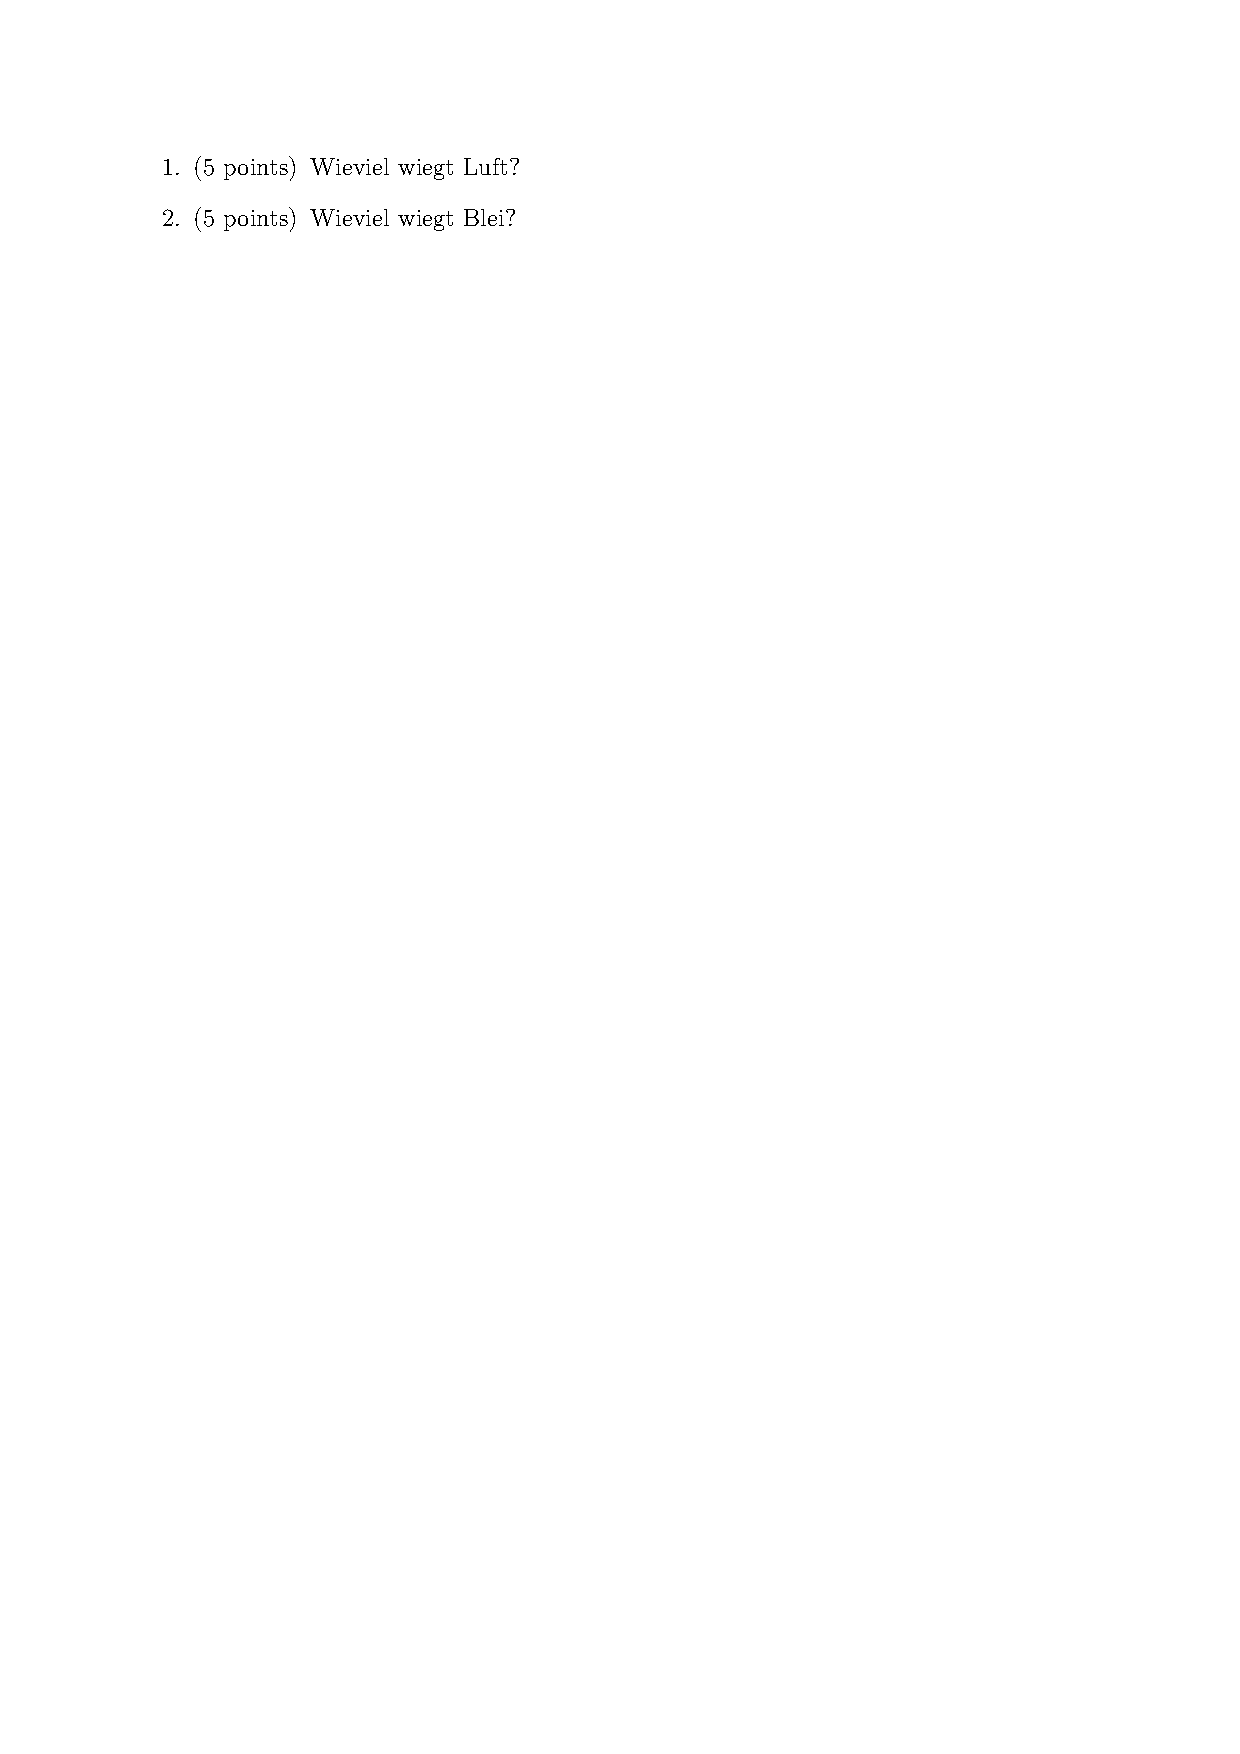
\includegraphics[clip,trim=2cm 25cm 6cm 1cm,width=\textwidth]{./Examples/exam/beispiel-01}}
\caption{Ergebnis von Listing \ref{lis:b01}, \texttt{beispiel-01.tex}}\label{fig:b01}
\end{figure}



\begin{lfgwcode}{label={lis:pak}}
\usepackage[ngerman]{babel} % ngerman mal nicht als Klassenoption
\usepackage[utf8]{inputenc}
\usepackage[T1]{fontenc}
\usepackage{booktabs} % schöne Tabellen
\usepackage{csquotes} % Anführungszeichen mit \enquote{}
\usepackage{paralist} % für kompakte Aufzählungen
\usepackage[math]{iwona} % Font mit Mathe-Support
\usepackage{amsmath,textcomp,tikz} %diverses
\usepackage{eso-pic} % Bilder im Hintergrund
\end{lfgwcode}


Die Anpassung der Begriffe geschieht in \texttt{exam} über spezielle Befehle, eine Auswahl der in späteren Beispielen notwendigen finden sich in Listing \ref{lis:lang}, die Dokumentation enthält noch eine Reihe anderer entsprechender Befehle.

\begin{lfgwcode}{label={lis:lang}}
\pointpoints{Punkt}{Punkte}
\bonuspointpoints{Bonuspunkt}{Bonuspunkte}
\renewcommand{\solutiontitle}{\noindent\textbf{Lösung:}\enspace}
 
\chqword{Frage}   
\chpgword{Seite} 
\chpword{Punkte}   
\chbpword{Bonus Punkte} 
\chsword{Erreicht}   
\chtword{Gesamt}

\hpword{Punkte:} % Punktetabelle
\hsword{Ergebnis:}
\hqword{Aufgabe:}
\htword{Summe:}
\end{lfgwcode}

Kombinieren wir nun die Paketliste aus Listing \ref{lis:pak} mit dem Minimalbeispiel aus Listing \ref{lis:b01}, so erhalten wir beim Übersetzen die Ausgabe von Abbildung \ref{fig:b02}.

\begin{figure}[b]
\fbox{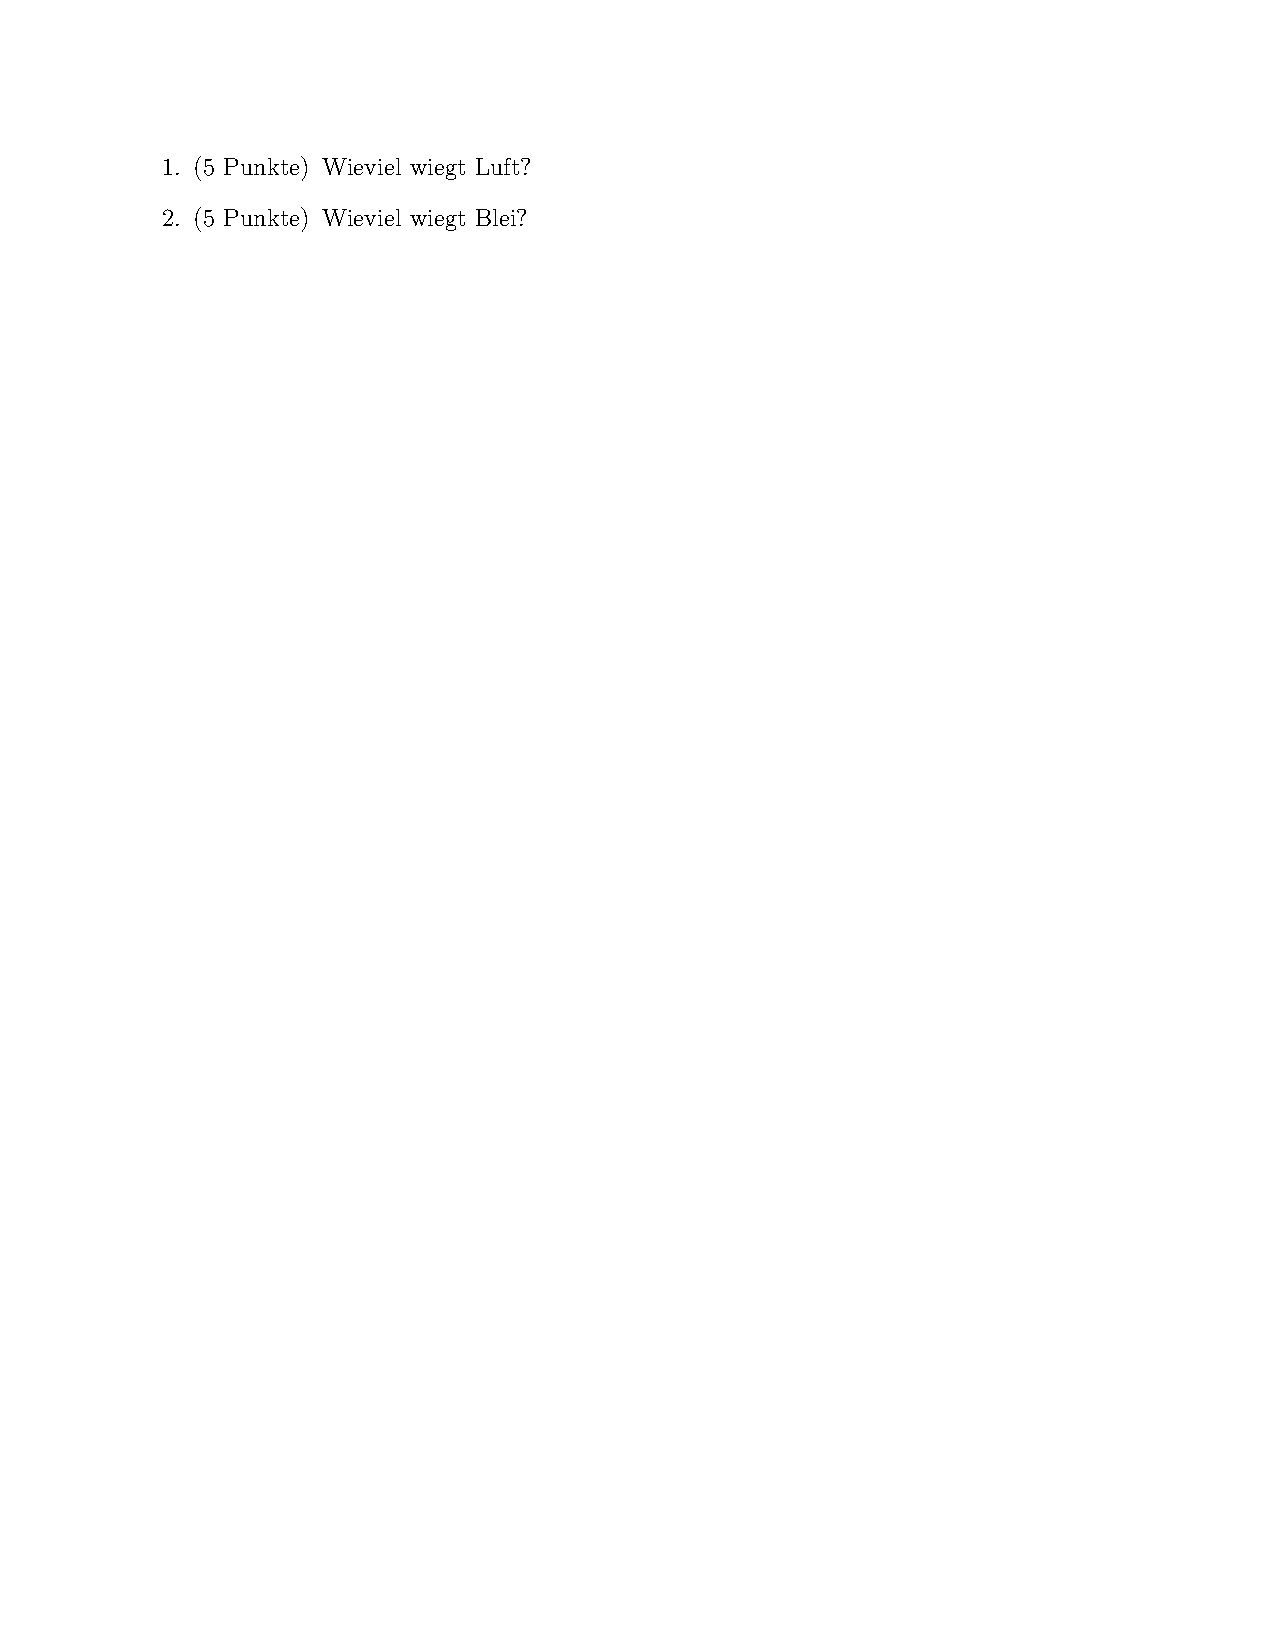
\includegraphics[clip,trim=1cm 22cm 8cm 1cm,width=\textwidth]{./Examples/exam/beispiel-02}}
\caption{Listings \ref{lis:b01} und \ref{lis:lang} kombiniert, \texttt{beispiel-02.tex}}\label{fig:b02}
\end{figure}

\section{Formatierung von Kopf \& Fuß}

\texttt{exam} bietet eine Reihe von Möglichkeiten für die Anpassung von Kopf und Fuß. 
Listing \ref{lis:headfoot} zeigt, wie \texttt{firstpageheader} und -\texttt{footer} für die Titelseite beziehungsweise \texttt{runningpageheader} und -\texttt{footer} für Folgeseiten mit Angabe von Fach und Dozent ausgestattet werden können.
Horizontale Linien unter den Kopfzeilen werden durch die entsprechenden \texttt{\dots headrule} Befehle gesetzt. 
Abbildung \ref{fig:headfoot} zeigt das entsprechende Ergebnis.

\begin{lfgwcode}{label={lis:headfoot}}
\newcommand{\dozent}{Dr. Uwe Ziegenhagen}
\newcommand{\fach}{Klausur Statistik}
 
\pagestyle{headandfoot}
\firstpageheadrule
\runningheadrule

\firstpageheader{}{}{\dozent \\ \fach}
\runningheader{}{}{\dozent \\ \fach}
\firstpagefooter{}{}{\thepage\,/\,\numpages}
\runningfooter{}{}{\thepage\,/\,\numpages}
\end{lfgwcode}

\begin{figure}[b]
\fbox{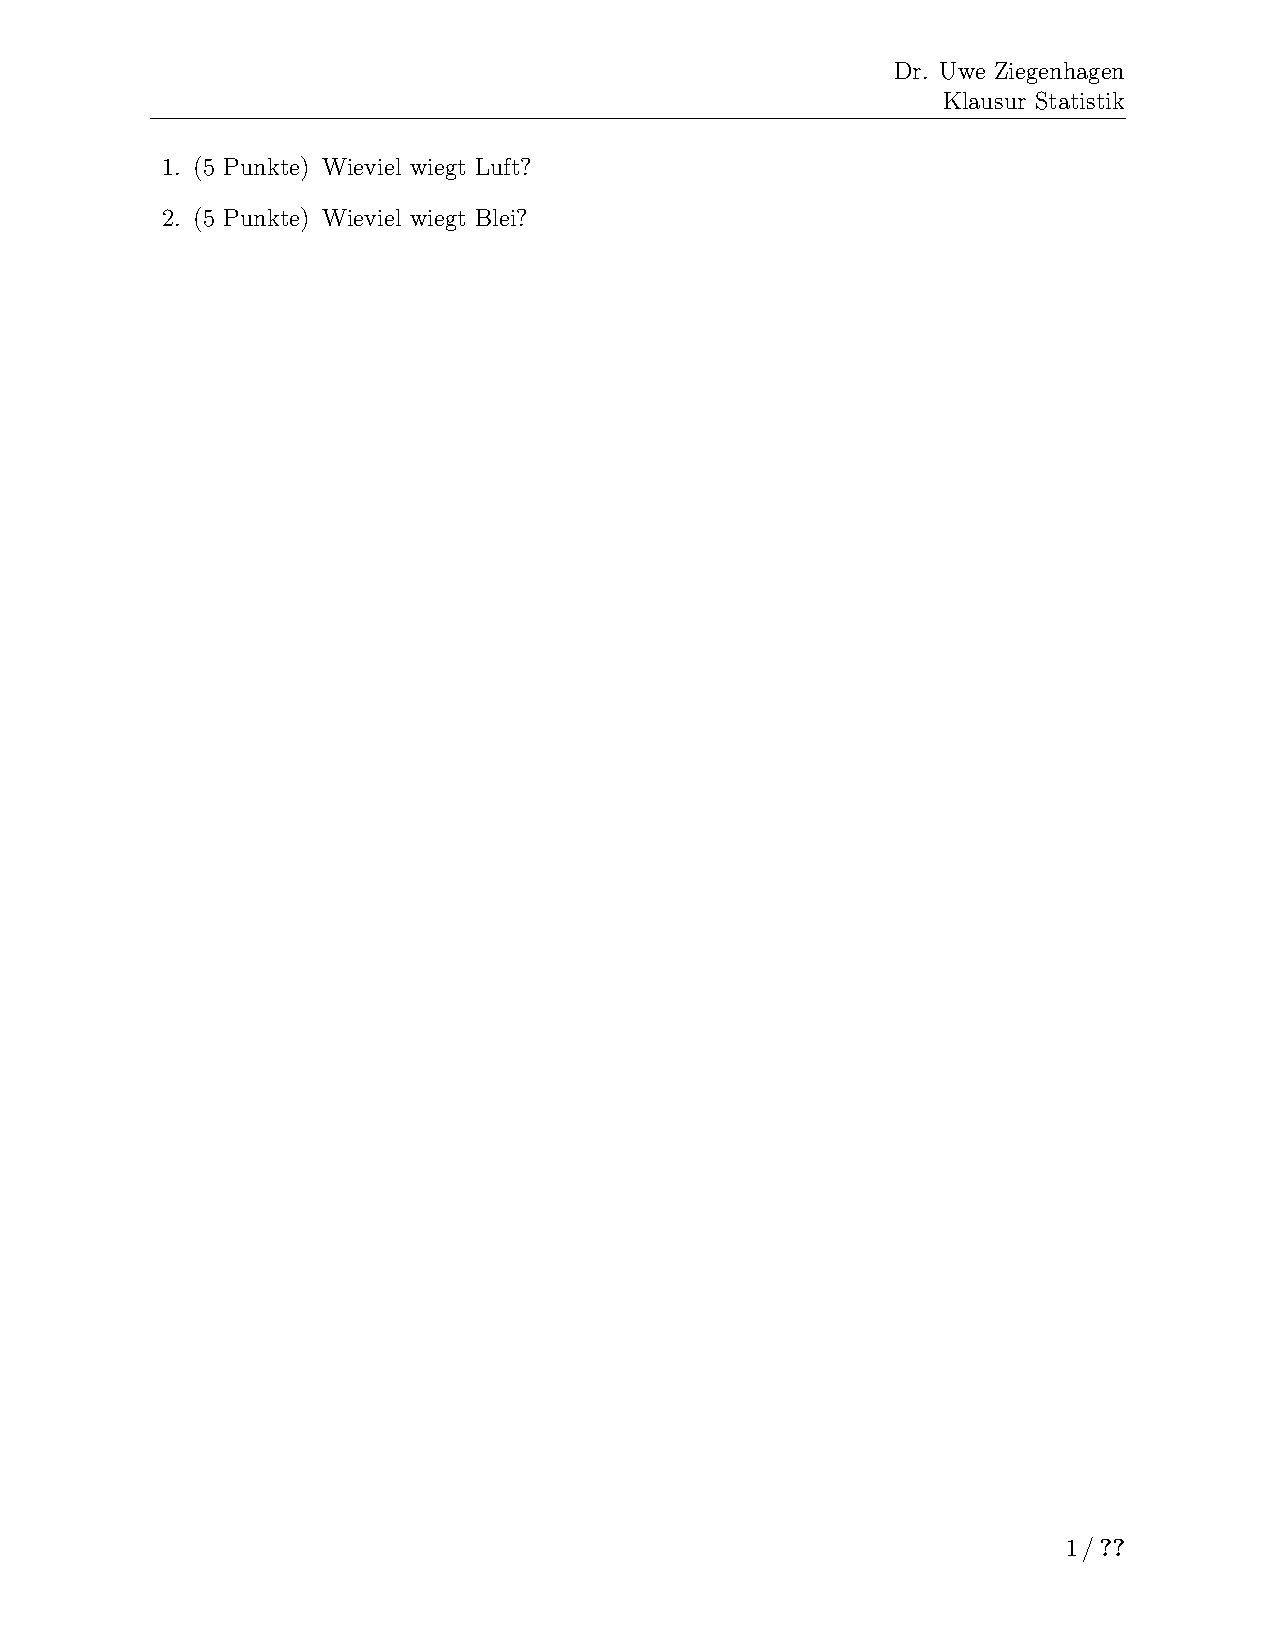
\includegraphics[trim=2cm 18cm 2cm 0.5cm,width=\textwidth]{./Examples/exam/beispiel-03}}
\caption{Ergebnis von Listing \ref{lis:headfoot}, \texttt{beispiel-03.tex}}\label{fig:headfoot}
\end{figure}

\clearpage

\section{Einfügen von Teilfragen}

Einzelne Fragen, die mit \texttt{\textbackslash question} gesetzt wurden, lassen sich noch in Unterfragen unterteilen. 
\paket{exam} bietet dazu folgende Umgebungen und dazugehörige Befehle an, die wie \texttt{\textbackslash question} zu nutzen sind:

\begin{itemize}
	\item \texttt{parts} Umgebung mit \texttt{\textbackslash part} Befehl
	\item \texttt{subparts} Umgebung mit \texttt{\textbackslash subpart} Befehl
	\item \texttt{subsubparts} Umgebung mit \texttt{\textbackslash subsubpart} Befehl
\end{itemize}

Listing \ref{lis:parts} zeigt, wie man eine Frage in zwei \texttt{\textbackslash part} Unterfragen unterteilt, Abbildung \ref{fig:allparts} die Ausgabe eines erweiterten Beispiels, das auch \texttt{\textbackslash subpart} und \texttt{\textbackslash subsubpart} nutzt.

\begin{lfgwcode}{label={lis:parts}}
\question[5]
Wieviel wiegt Luft?

\begin{parts}
\part[3] Geben Sie den Wert in Gramm pro Kubikmeter an!

\part[2] Geben Sie den Wert in Kilogramm pro Kubikkilometer an!
\end{parts}
\end{lfgwcode}


\begin{figure}[b]
\fbox{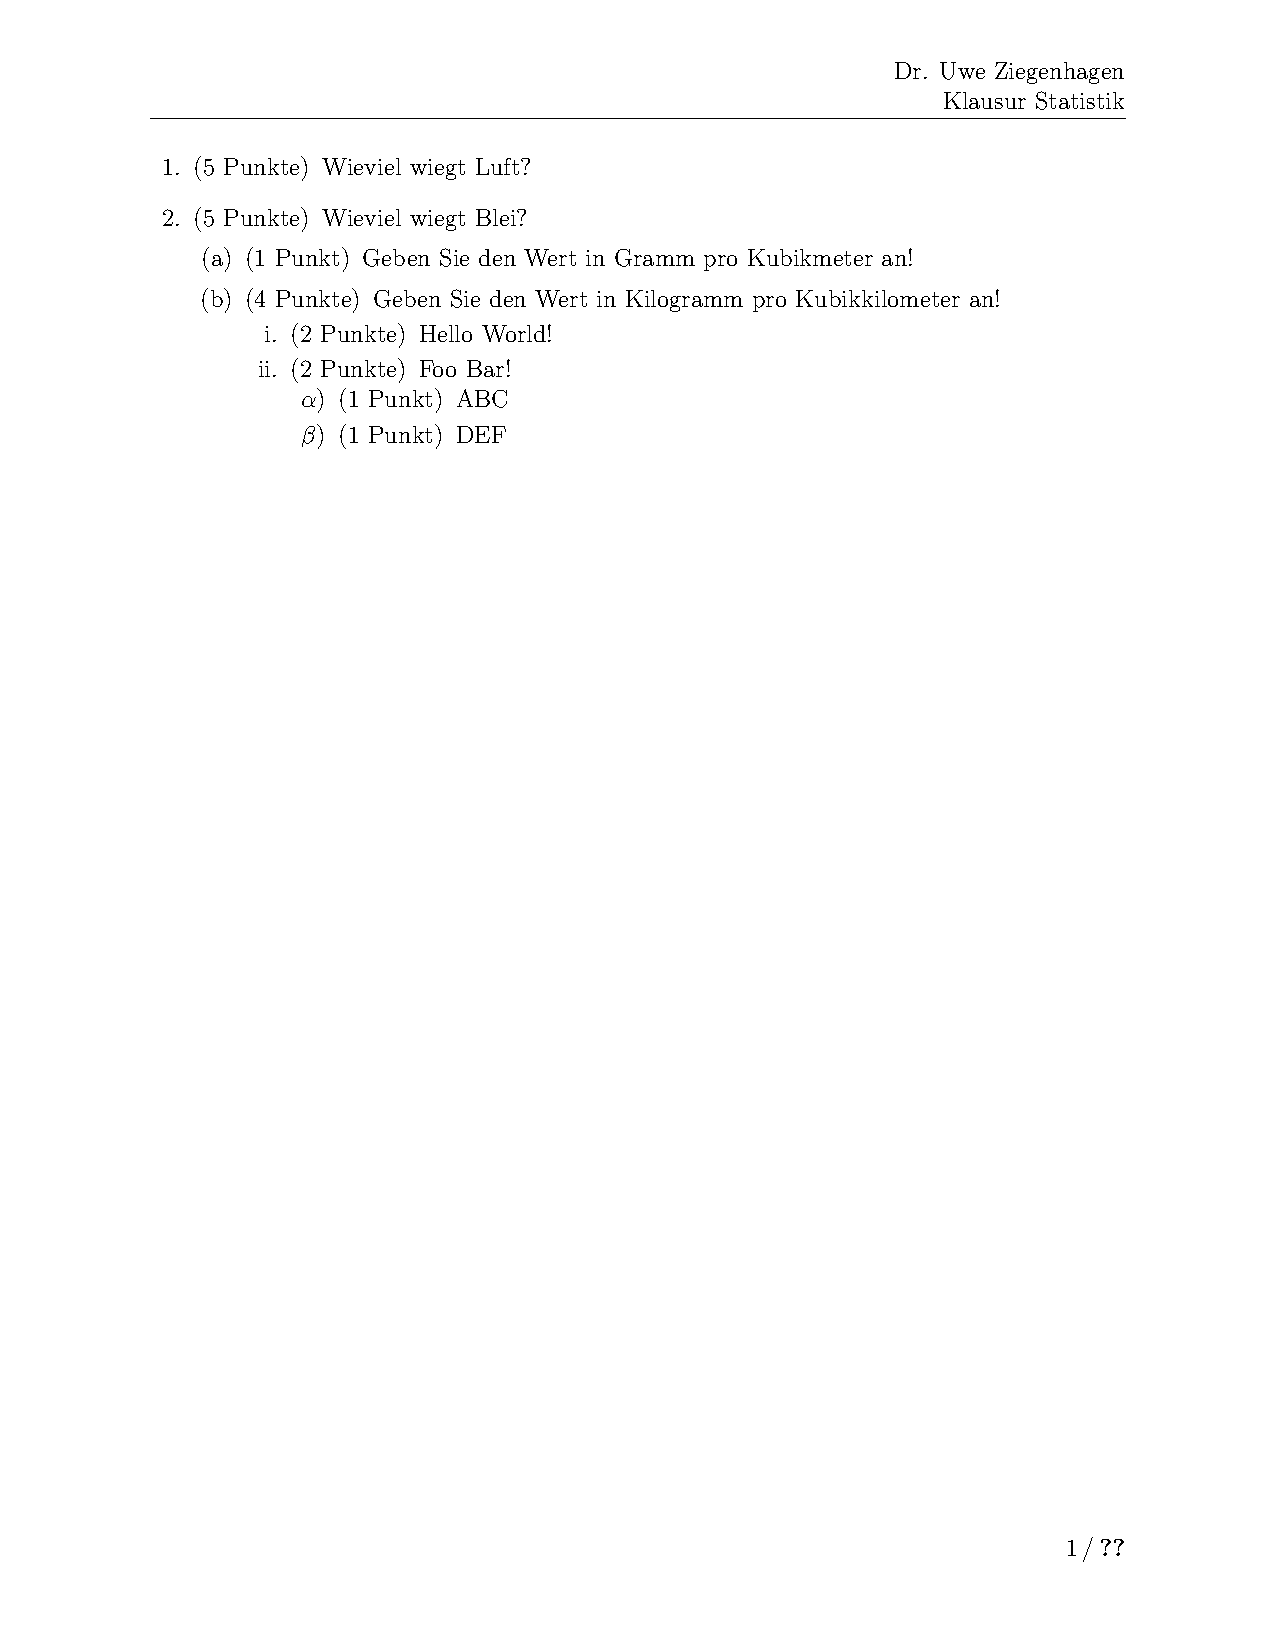
\includegraphics[trim=2cm 19cm 2cm 0.5cm,width=\textwidth]{./Examples/exam/beispiel-04}}
\caption{Ergebnis von Listing \ref{lis:parts}, \texttt{beispiel-04.tex}}\label{fig:allparts}
\end{figure}


\section{Weitere Aufgabentypen}

Neben Textaufgaben unterstützt \texttt{exam} auch sogenannte Multiple-Choice Aufgaben und Lückentexte. 
Es stellt dazu folgende Umgebungen bzw. Befehle bereit:

\begin{description}
\item[choices] Umgebung, stellt dem Eintrag einen Buchstaben voran
\item[checkboxes] Umgebung, nutzt keinen Buchstaben sondern einen  Kreis, der angekreuzt werden kann
\item[oneparcheckboxes] Umgebung wie \texttt{checkboxes}, jedoch in einem Absatz nebeneinander anstatt untereinander
\item[fillin] Befehl für Lückentext, als optionaler Parameter wird das Lösungswort übergeben
\end{description}

Für die drei genannten Umgebungen gilt, dass die jeweils richtige Antwort bzw. die richtigen Antworten mittels \texttt{\textbackslash CorrectChoice} von den falschen Antworten unterschieden werden können. 
Setzt man die \enquote{answers} Option wie oben beschrieben als Klassenoption, so werden diese richtigen Antworten entsprechend markiert. 
Listing \ref{lis:mchoice1} und \ref{lis:mchoice2} zeigen die entsprechenden Code-Beispiele, Abbildung \ref{fig:mchoicea} die Ausgabe mit \enquote{answers} aktiviert.

\begin{lfgwcode}{label={lis:mchoice1}}
\question Wer war kein Beatle?

\begin{choices}
\choice John
\choice Paul
\choice George
\choice Ringo
\CorrectChoice Socrates
\end{choices}

\question Wer war kein Beatle?

\begin{checkboxes}
\choice John
\choice Paul
\choice George
\choice Ringo
\CorrectChoice Socrates
\end{checkboxes}
\end{lfgwcode}

\clearpage

\begin{lfgwcode}{label={lis:mchoice2}}

\question Wer war kein Beatle?

\begin{oneparcheckboxes}
\choice John
\choice Paul
\choice George
\choice Ringo
\CorrectChoice Socrates
\end{oneparcheckboxes}

\question \fillin[James Bond] ist der coolste Superheld.

\end{lfgwcode}

\begin{figure}
\fbox{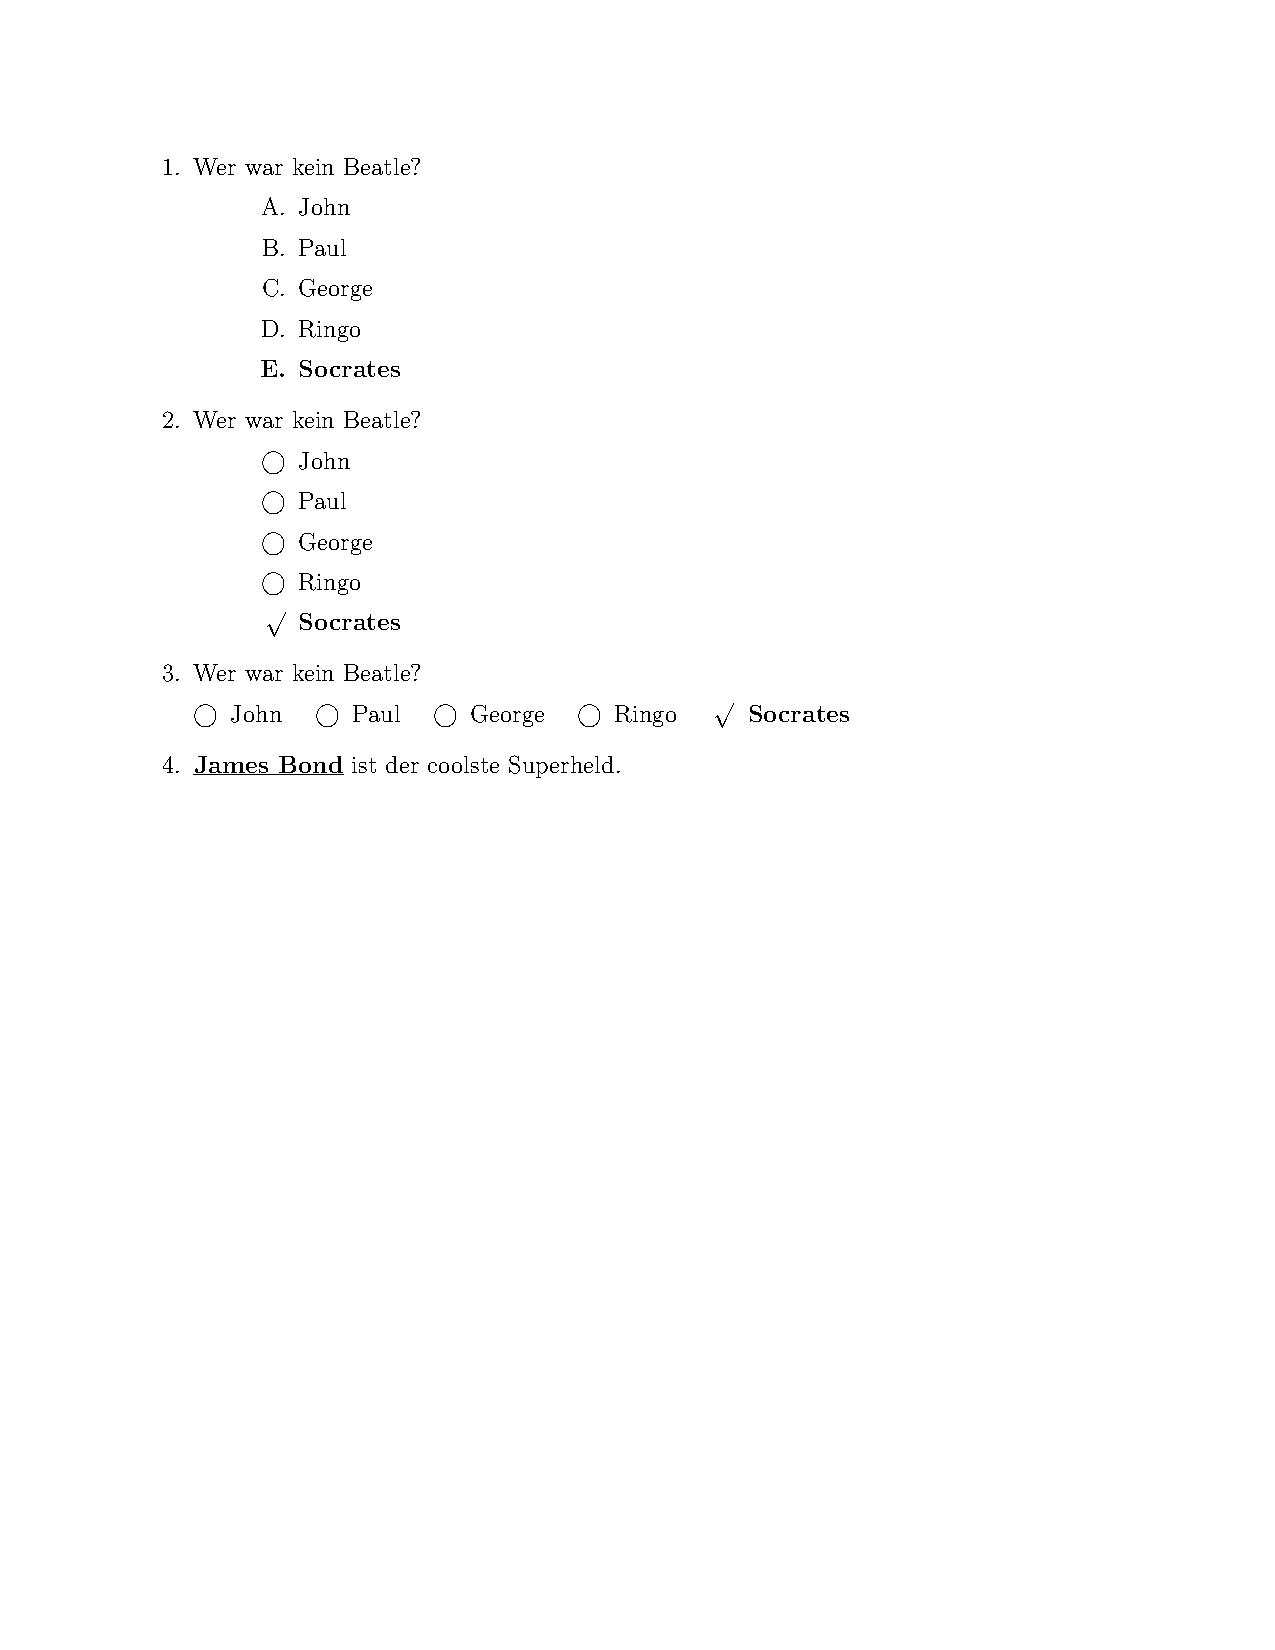
\includegraphics[trim=1cm 13.5cm 3cm 1cm,width=0.95\textwidth]{./Examples/exam/beispiel-06}}
\caption{Listings \ref{lis:mchoice1} und \ref{lis:mchoice2} kombiniert, \texttt{beispiel-06.tex}}\label{fig:mchoicea}
\end{figure}

\clearpage

\section{Platz für Antworten}

\texttt{exam} erlaubt es dem Dozenten auch, unterschiedliche Leerräume für die Antworten von Schülern und Studenten bereitzuhalten. 
Neben einfachem Leerraum mittels \texttt{\textbackslash vspace} und umrahmten Boxen mittels (siehe Listing \ref{lis:vspace1} sowie die Ausgabe in Abbildung \ref{fig:vspace1}) stellt \texttt{exam} auch linierte und gepunktete Linien sowie karierten Platz bereit.

\begin{lfgwcode}{label={lis:vspace1}}
% einfacher Abstand
\vspace{<Länge>}

%bis zum Seitenende
\vspace*{\stretch{1}}
\newpage

% leere umrahmte Box
\makeemptybox{<Länge>}

%leere umrahmte Box bis zum Seitenende
\makeemptybox{\stretch{1}}
\newpage
\end{lfgwcode}

\begin{figure}[b]
\fbox{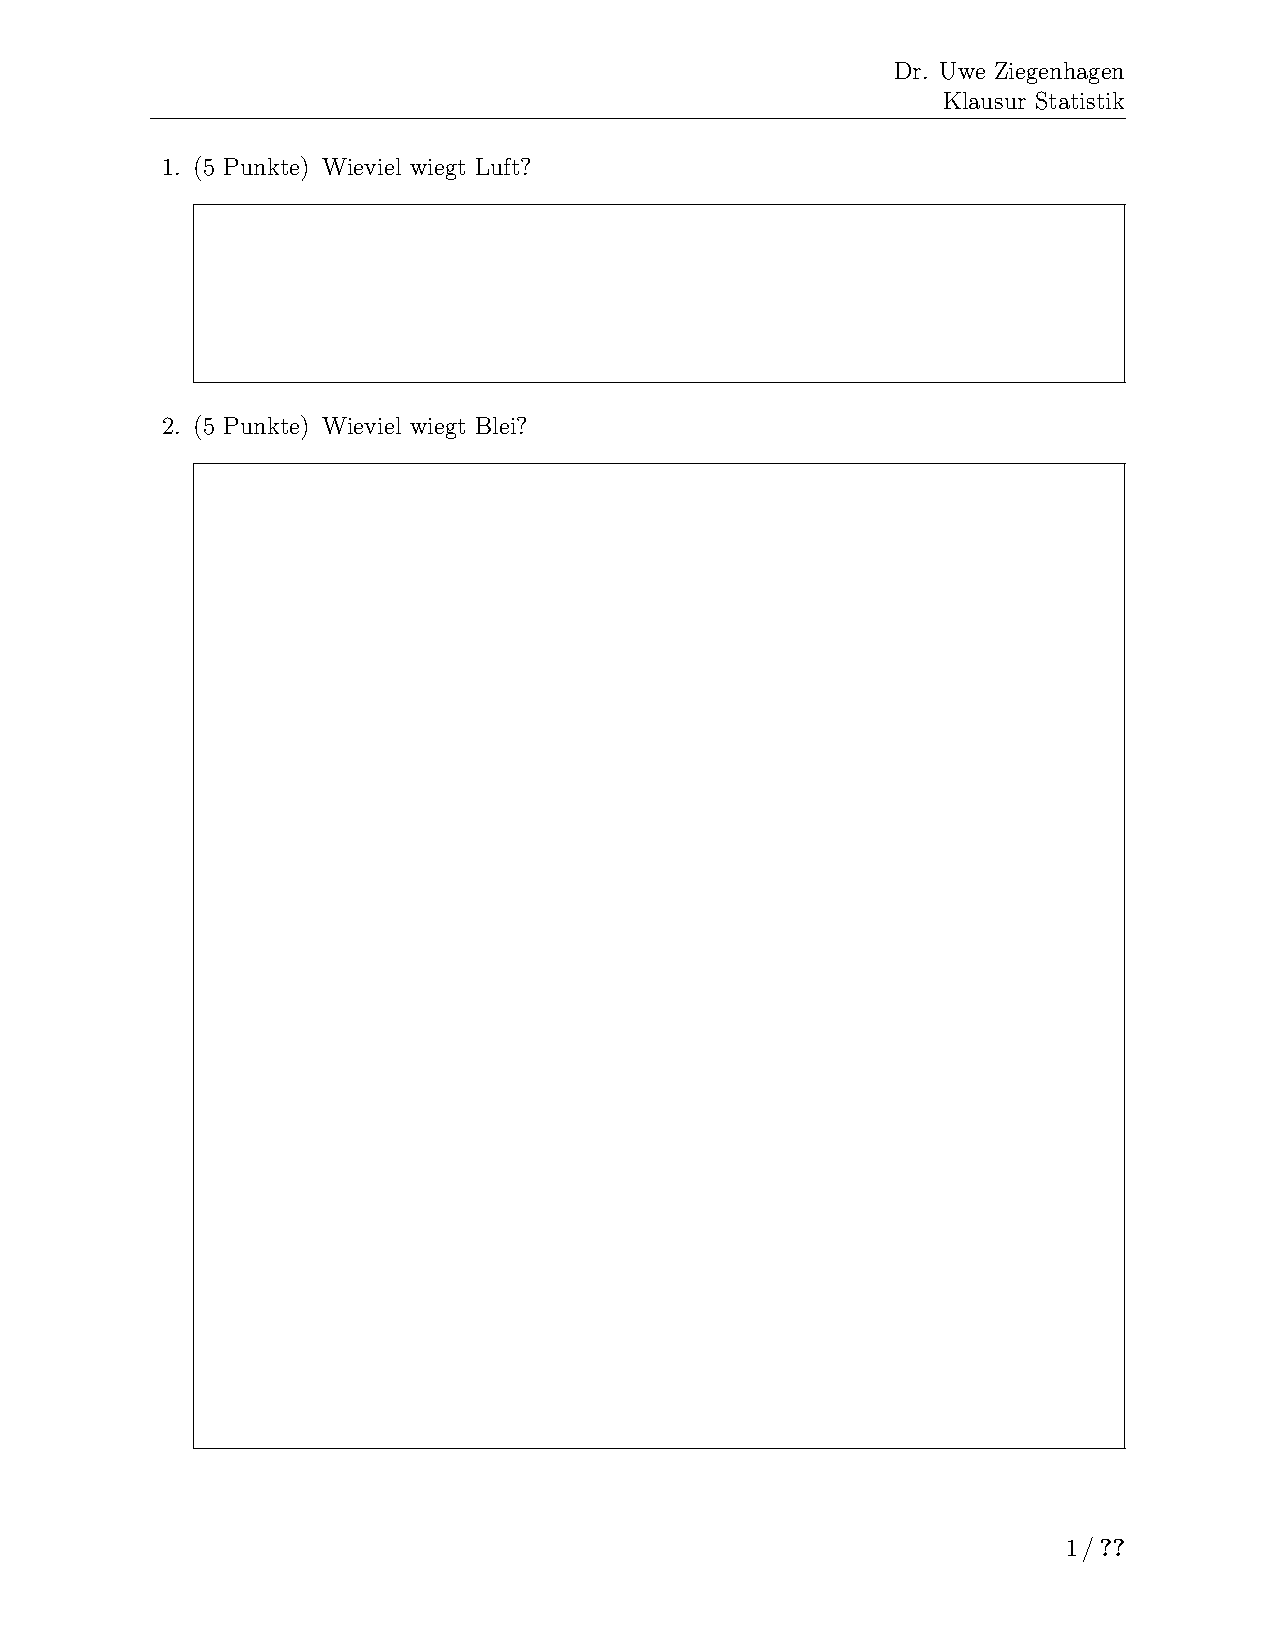
\includegraphics[clip, trim=2cm 17cm 1.5cm 2.5cm,width=\textwidth]{./Examples/exam/beispiel-07}} % 
\caption{Ergebnis von Listing \ref{lis:vspace1}, \texttt{beispiel-07.tex}}\label{fig:vspace1}
\end{figure}

Für Linien nutzt man \texttt{\textbackslash fillwithlines}, für gepunktete Linien \texttt{\textbackslash fillwithdottedlines}, und für ein kariertes Raster \texttt{\textbackslash fillwithgrid}. 
Alle drei Befehle benötigen als Parameter die vertikale Länge des Platzes, den sie für die Antworten reservieren sollen. 
Außerdem stellt \texttt{exam} noch den \texttt{\textbackslash answerline} Befehl bereit, der Platz für ein Wort oder einen Satz schafft, der optional für die Lösungsausgabe angegeben werden kann.

Beispiele für die Nutzung dieser Befehle finden sich in Listing \ref{lis:fill}, für die Ausgaben siehe die Abbildungen \ref{fig:fill1} und \ref{fig:fill2}. 

\begin{lfgwcode}{label={lis:fill}}
\fillwithlines{<Länge>} % für linierten Platz
% Hinweis: \linefillheight für Abstand zwischen Linien

\fillwithdottedlines{<Länge>} % für gepunktete Linien
% Hinweis: Abstand in \dottedlinefillheight

\fillwithgrid{<Länge>} % 
% \setlength{\gridsize}{5mm}
% \setlength{\gridlinewidth}{0.1pt}

\answerline[Antwort] % für kurze Antworten
\end{lfgwcode}

\begin{figure}[b]
\fbox{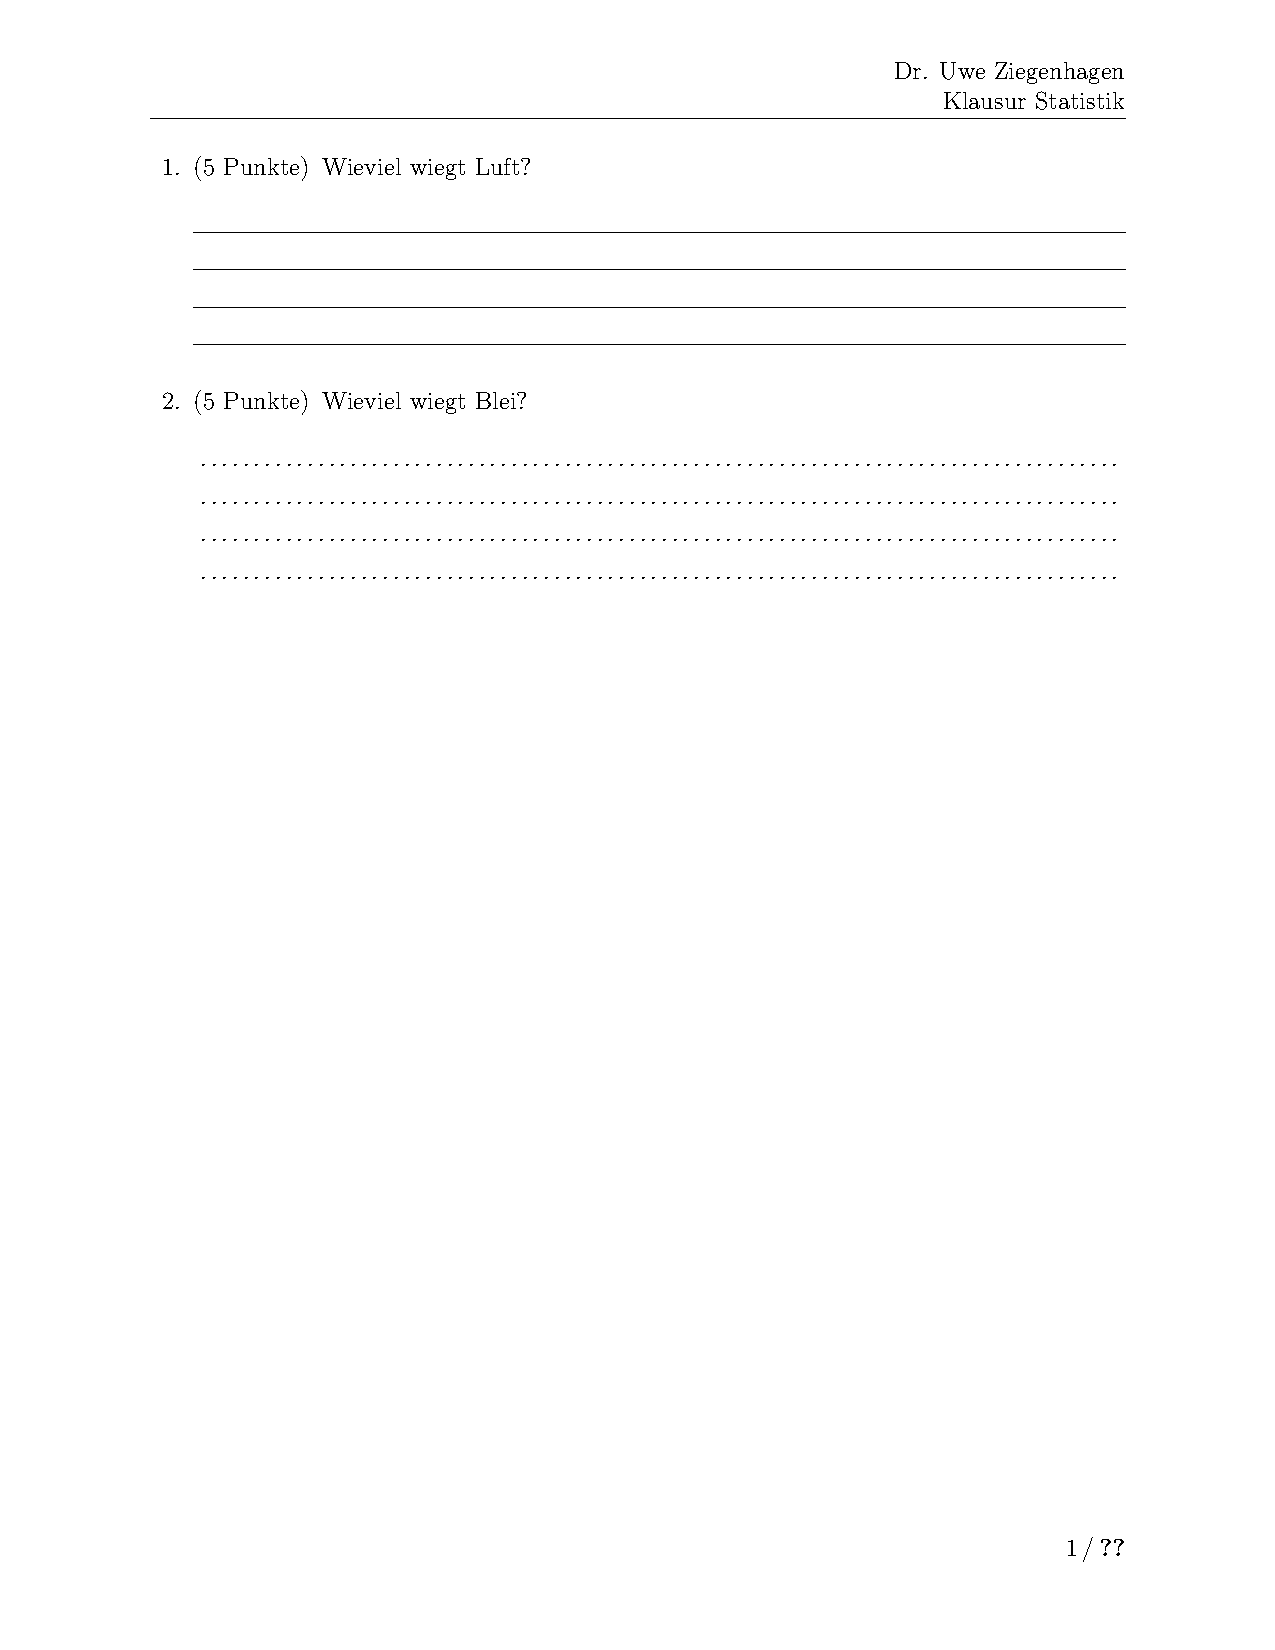
\includegraphics[clip, trim=2cm 16.5cm 2cm 2.5cm,width=\textwidth]{./Examples/exam/beispiel-08}} % 
\caption{Ausgabe von Listing \ref{lis:fill}, Teil 1}\label{fig:fill1}
\end{figure}

\begin{figure}
\fbox{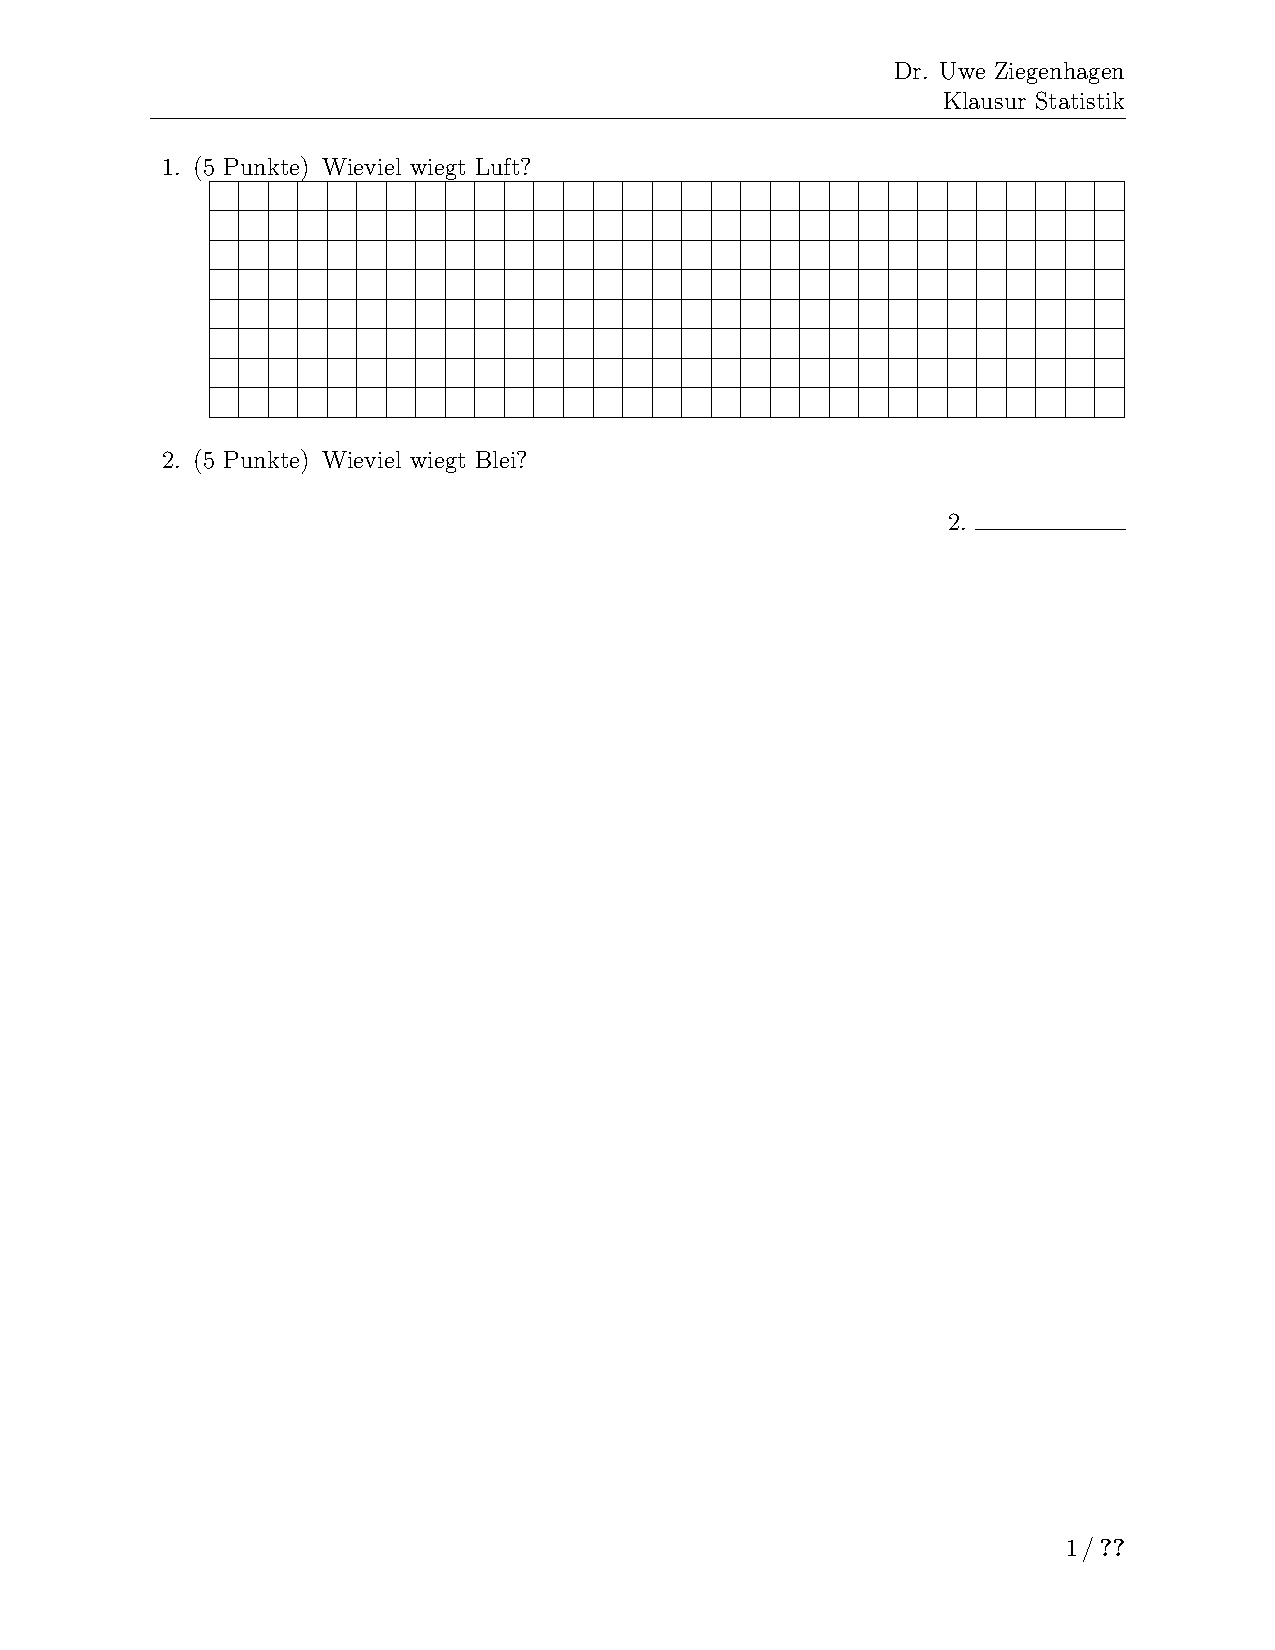
\includegraphics[clip, trim=2cm 18cm 2cm 2.5cm,width=\textwidth]{./Examples/exam/beispiel-09}} % 
\caption{Ausgabe von Listing \ref{lis:fill}, Teil 2}\label{fig:fill2}
\end{figure}

\section{Ausgabe von Lösungen}

Wie bereits erwähnt, steuert die globale Option \enquote{answers}, ob die hinterlegten Lösungen angezeigt werden sollen oder nicht. 
Die Hinterlegung von Lösungen bei Textaufgaben im Text erfolgt dabei über eingefügte \texttt{solution} Umgebungen, die hinter jede \texttt{\textbackslash question} gesetzt werden.
Listing \ref{lis:sol1} zeigt ein entsprechendes Beispiel, Abbildung \ref{fig:sol2} die entsprechende Ausgabe.

\begin{lfgwcode}{label={lis:sol1}}
\question Was ist die Antwort auf alle Fragen?

\begin{solution}
42
\end{solution}
\end{lfgwcode}

\begin{figure}
\fbox{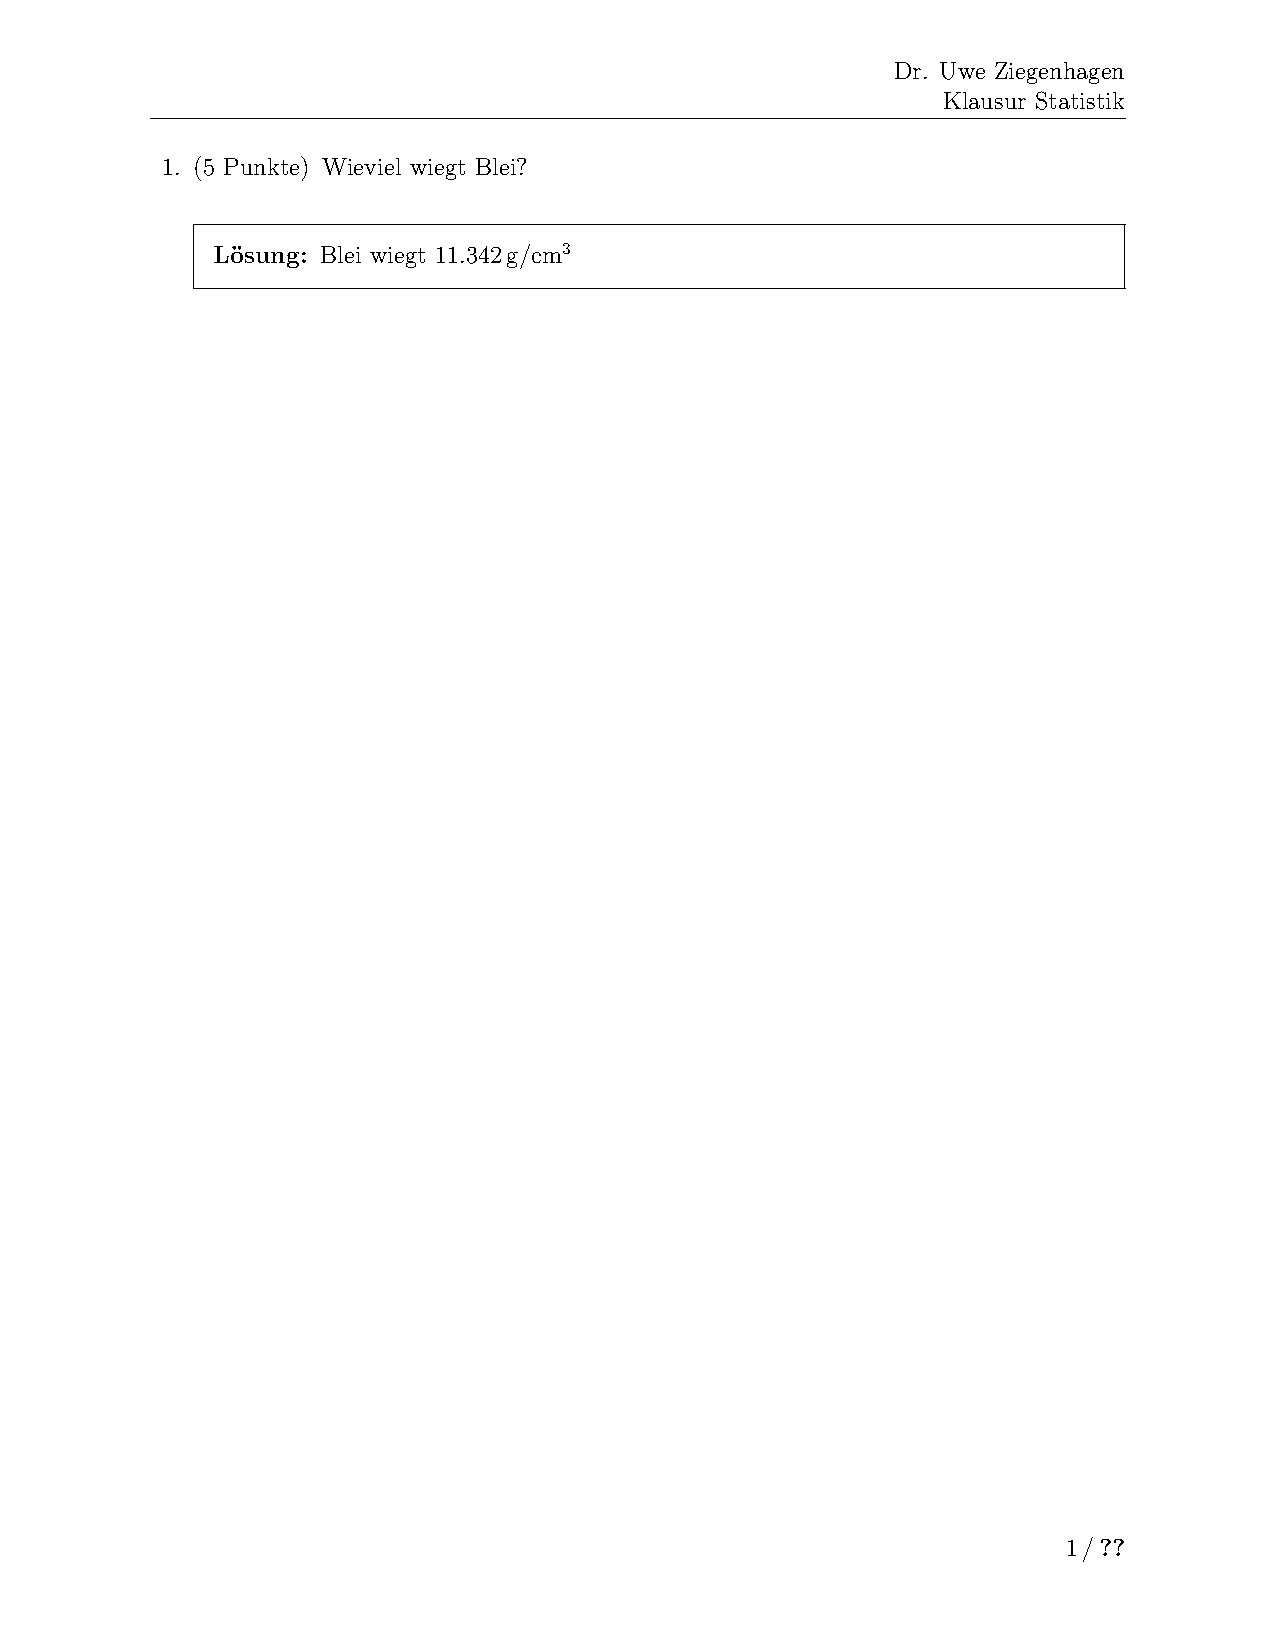
\includegraphics[clip, trim=2cm 22.5cm 2cm 0.7cm,width=\textwidth]{./Examples/exam/beispiel-10}} % 
\caption{Beispiel für die \texttt{solution} Umgebung}\label{fig:sol2}
\end{figure}

Alternativ biete das \texttt{exam} Paket auch die Möglichkeit, je nach gesetzter \enquote{answers} Option entweder die hinterlegte Lösung oder den Platz für die Antworten zu hinterlegen. 
Dazu stellt \texttt{exam} die folgenden Umgebungen bereit, deren jeweilige Bedeutung sich leicht aus dem Namen erschließt:

\begin{itemize}
	\item solutionorbox
	\item solutionorlines
	\item solutionordottedlines
	\item solutionorgrid
\end{itemize}

Die Abbildungen \ref{fig:solbox1} und \ref{fig:solbox2} zeigen am Beispiel von \texttt{solutionorgrid}, wie dies aussehen kann. Abbildung \ref{fig:solbox1} zeigt ein Gitter an, in das die Schüler die Lösung zeichnen können, Abbildung \ref{fig:solbox2} die Version mit Lösung\footnote{Für den Plot siehe \url{http://tex.stackexchange.com/questions/226277/how-to-plot-a-quadratic-equation-in-tikz}}.

\begin{figure}
\fbox{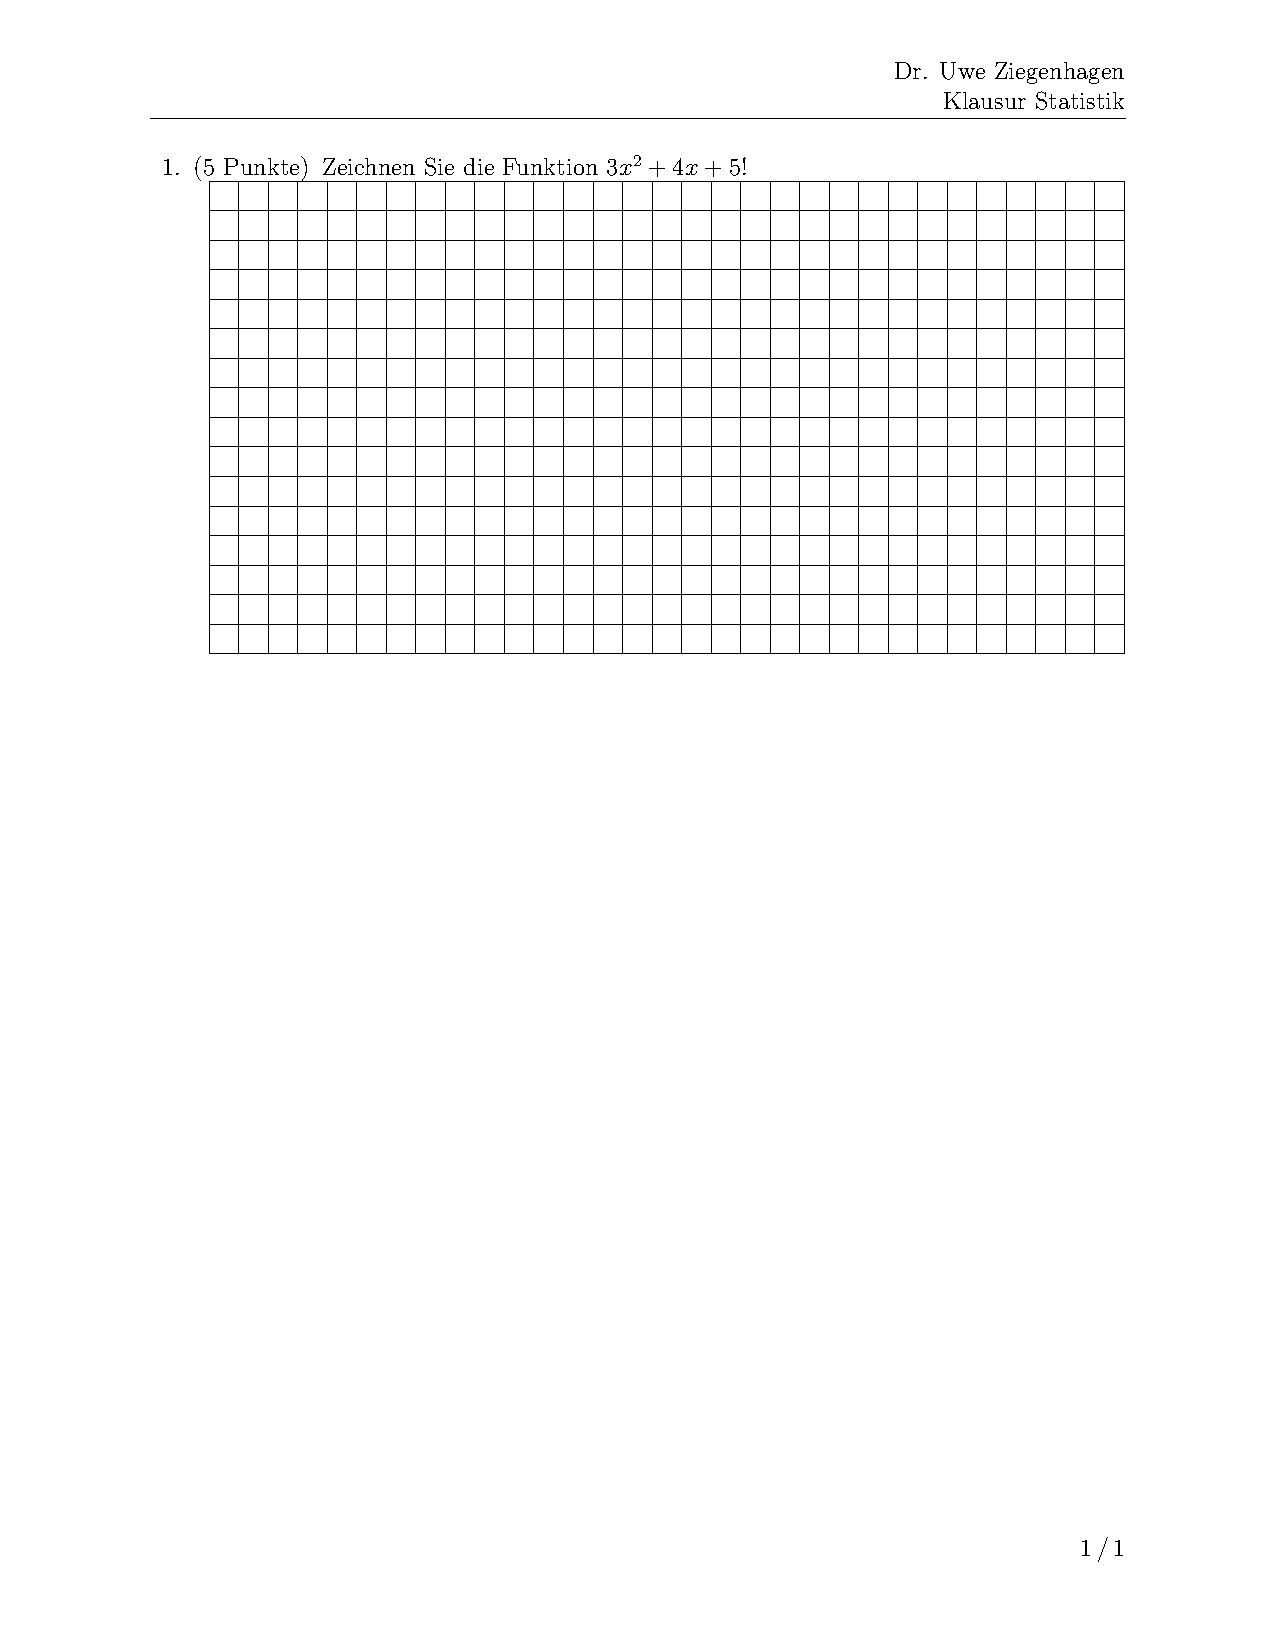
\includegraphics[clip, trim=2cm 16.5cm 2cm 0.7cm,width=\textwidth]{./Examples/exam/beispiel-11}} % 
\caption{Ausgabe von \texttt{\textbackslash solutionorgrid} ohne gesetztes \enquote{answers}}\label{fig:solbox1}
\end{figure}

\begin{figure}
\fbox{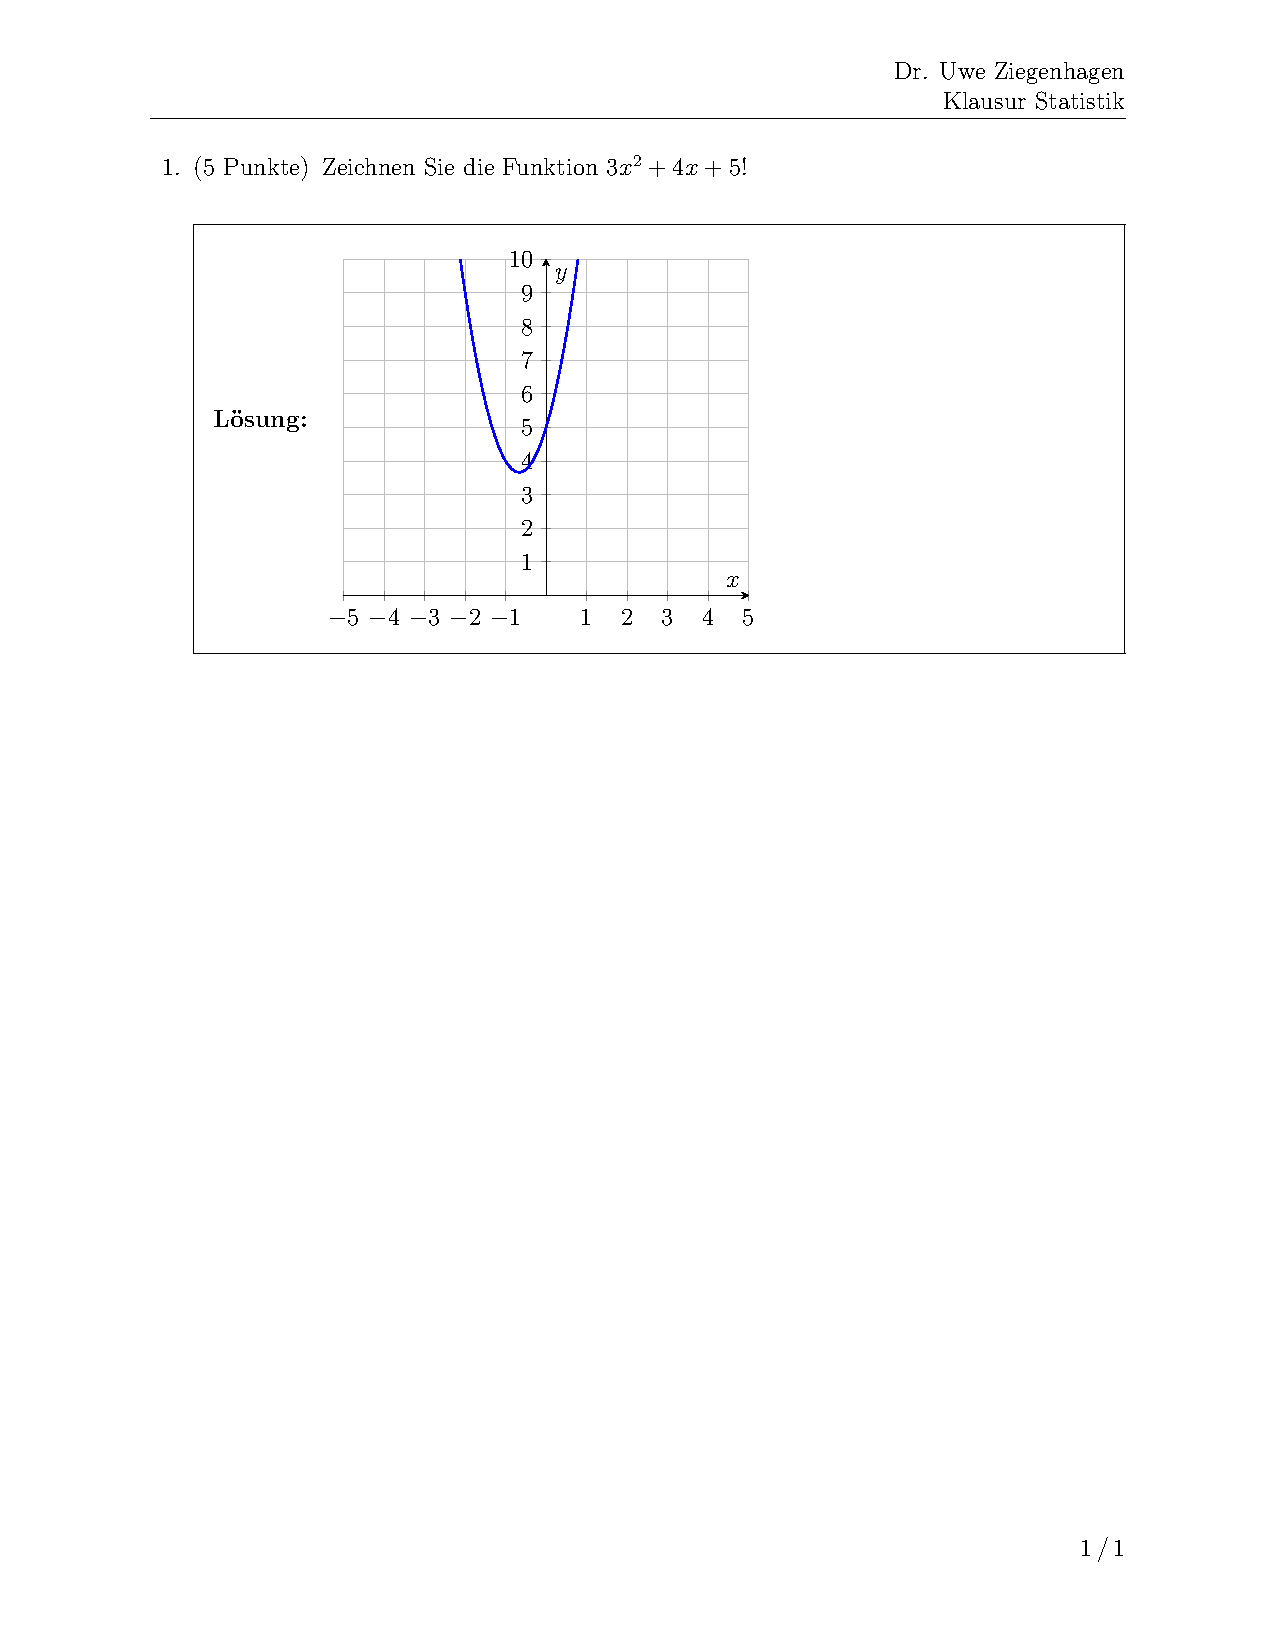
\includegraphics[clip, trim=2cm 15.5cm 2cm 0.7cm,width=\textwidth]{./Examples/exam/beispiel-12}} % 
\caption{Ausgabe von \texttt{\textbackslash solutionorgrid} mit gesetztem \enquote{answers}}\label{fig:solbox2}
\end{figure}

\section{Ausgabe von Notentabellen}

Wie bereits erwähnt kann \texttt{exam} auch Bewertungstabellen setzen, vertikal und horizontal, nach Aufgaben und nach Seiten. Listing \ref{lis:bew} zeigt die entsprechenden Befehle, die Abbildungen \ref{fig:hor} und \ref{fig:ver} zeigen jeweilige Ausgaben für horizontale Tabellen nach Fragen und Seiten.

\begin{lfgwcode}{label={lis:bew}}
\gradetable[v][questions] vertikal nach Fragen
\gradetable[h][questions] horizontal nach Fragen
\gradetable[v][pages] vertikal nach Seiten
\gradetable[h][pages] horizontal nach Seiten
\end{lfgwcode}

\begin{figure}[b]
\fbox{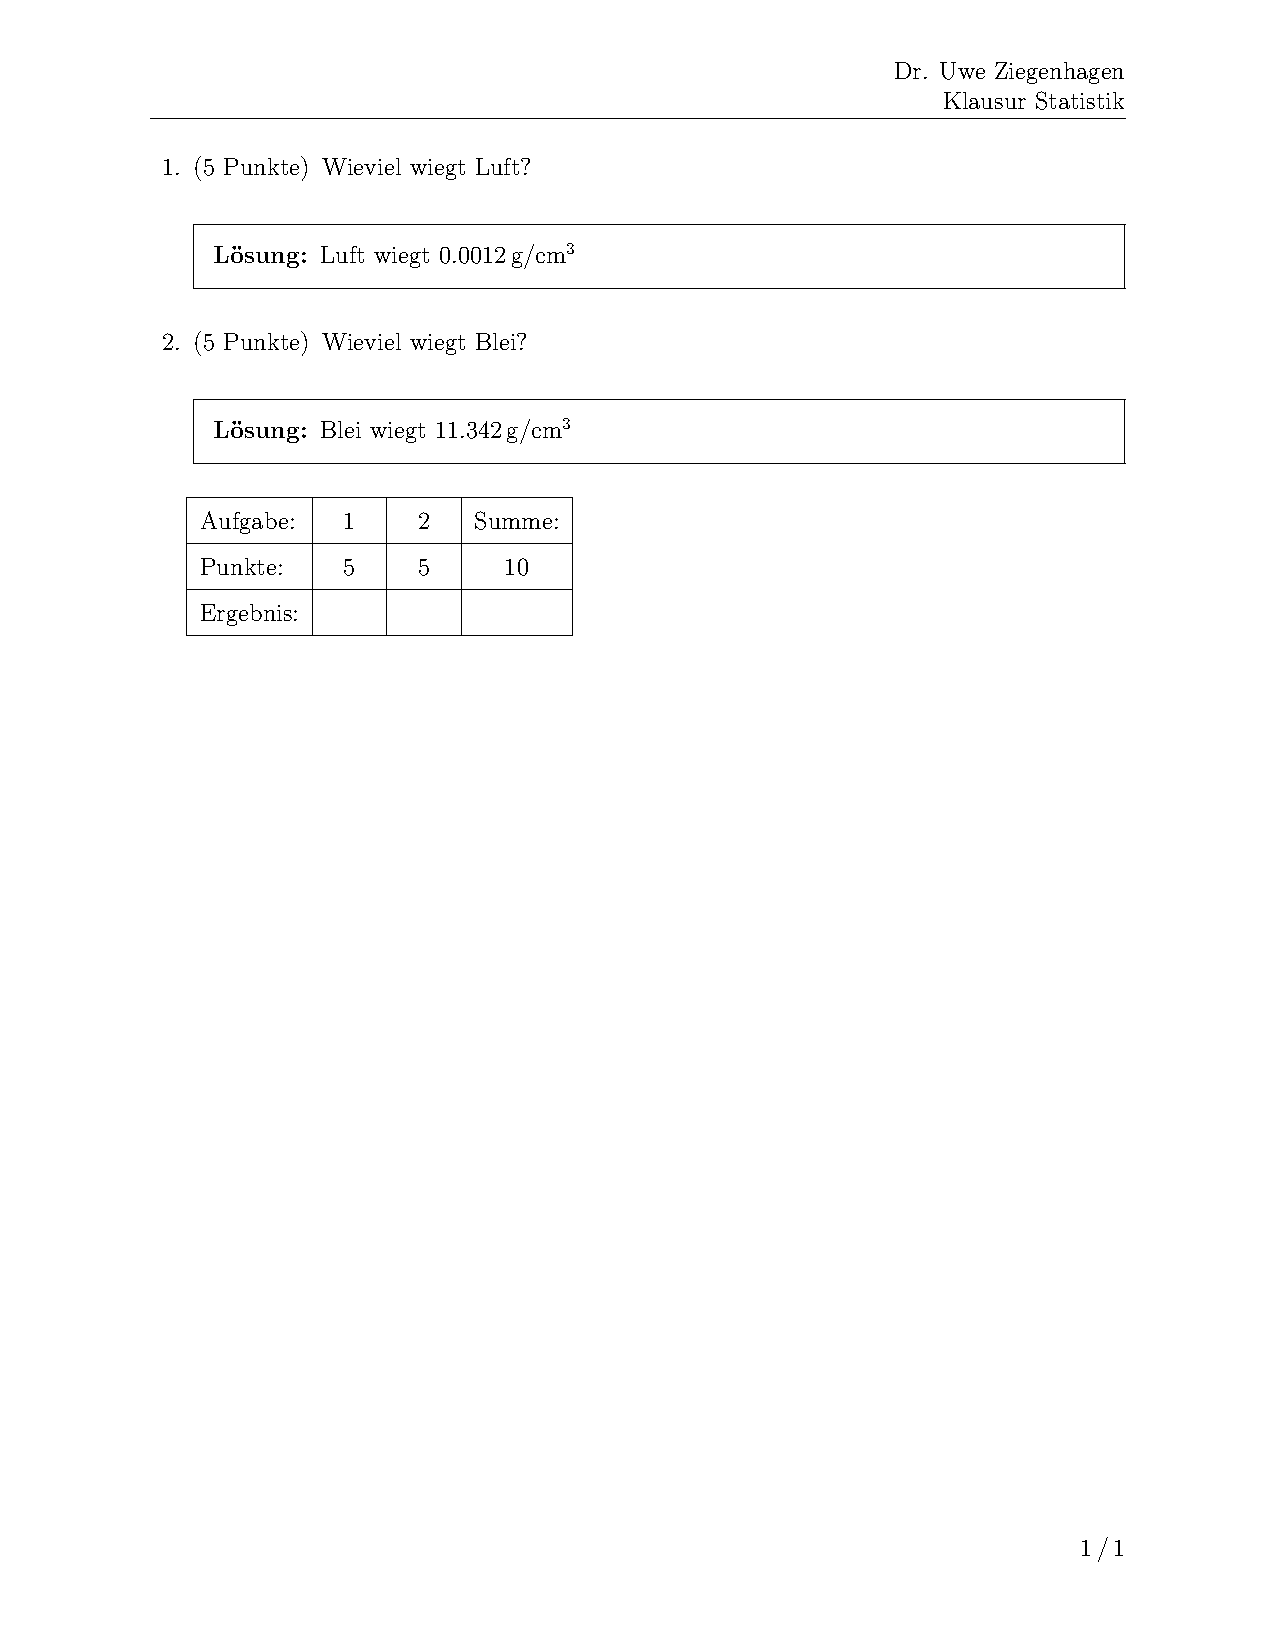
\includegraphics[clip, trim=2.5cm 15cm 2.5cm 0.7cm,width=\textwidth]{./Examples/exam/beispiel-13}} % 
\caption{Bewertungstabelle horizontal nach Fragen}\label{fig:hor}
\end{figure}

\begin{figure}
\fbox{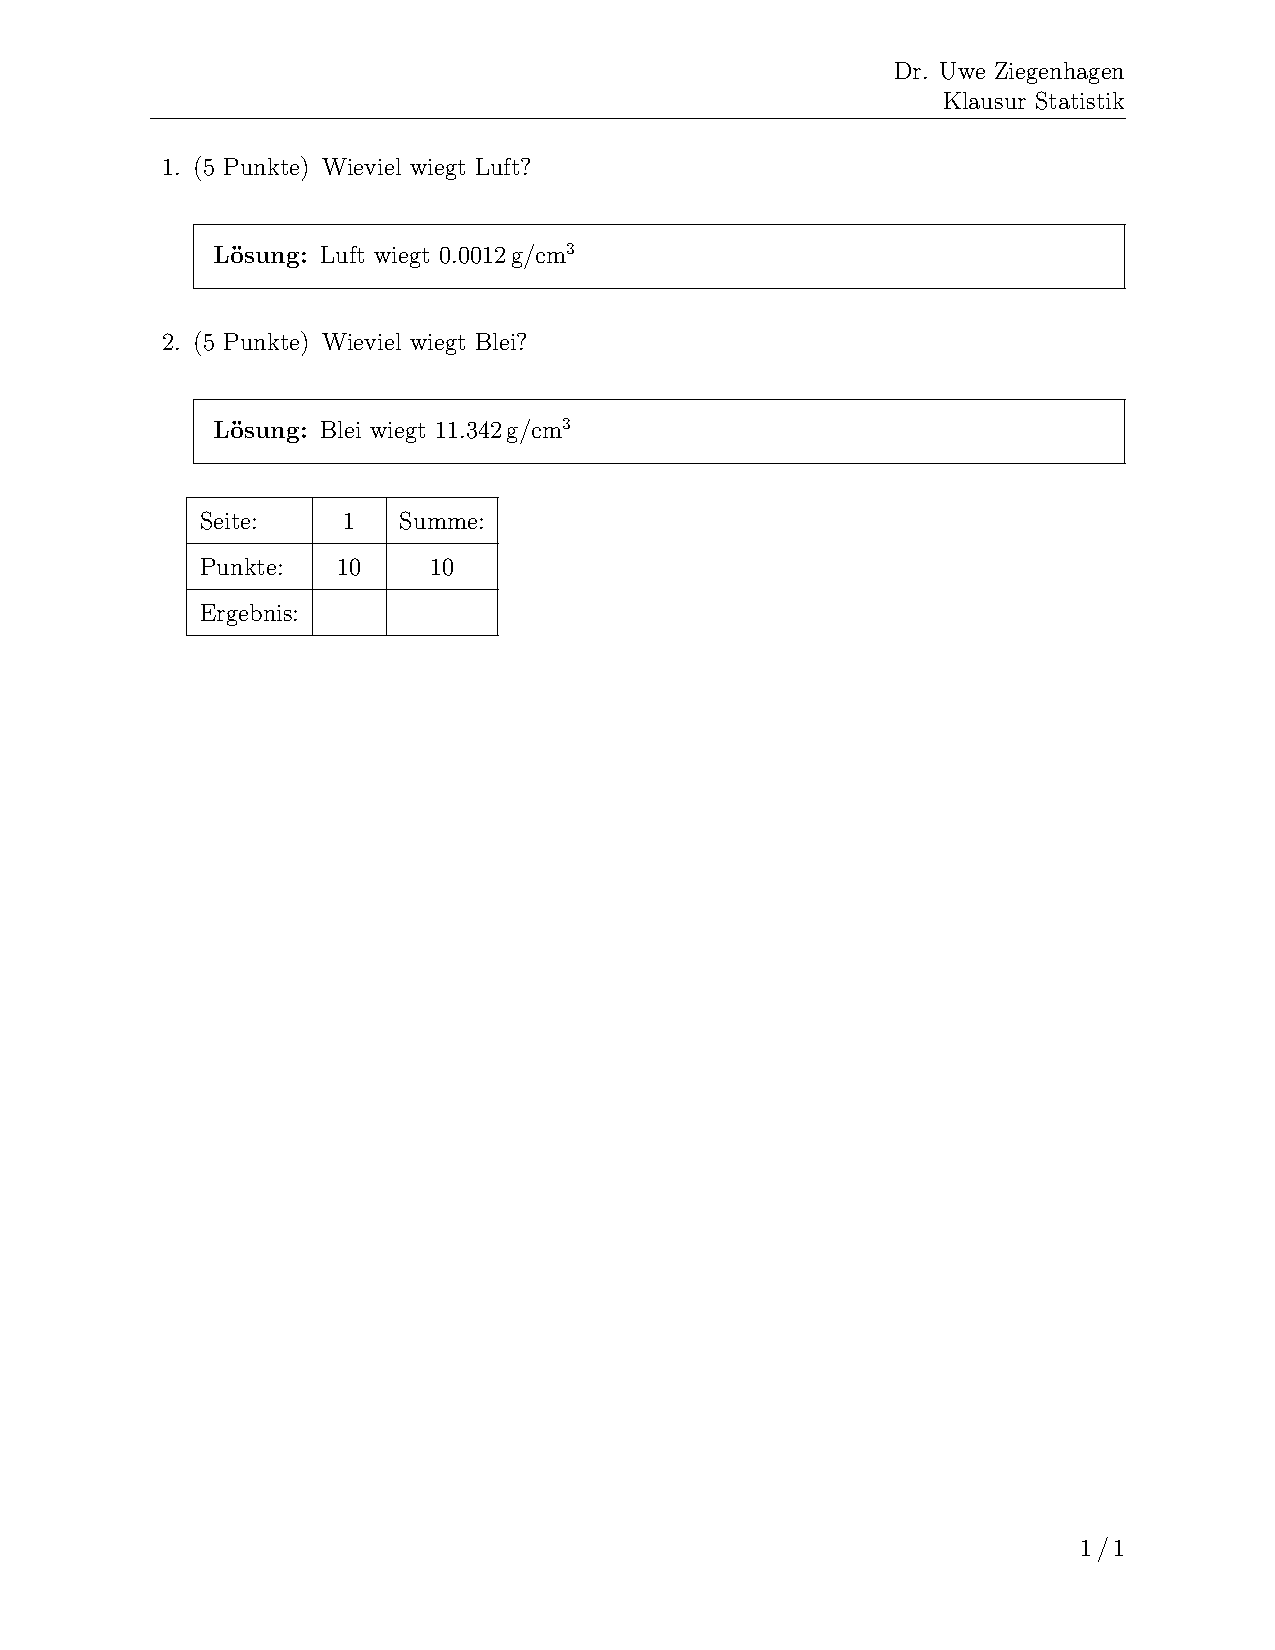
\includegraphics[clip, trim=2.5cm 17cm 2.5cm 0.7cm,width=\textwidth]{./Examples/exam/beispiel-14}} % 
\caption{Bewertungstabelle horizontal nach Seiten}\label{fig:ver}
\end{figure} 


\paket{exam} bietet noch mehr, als diese kurze Einführung zeigen konnte, interessierten Lesern möchte ich daher nochmals die Dokumentation zum Paket empfehlen. 
% !TEX root = lfgw.tex
\chapter{Präsentationen mit Beamer}
\autor{Axel Kielhorn}

\noindent Die Beamer Klasse bietet eine einfache Möglichkeit Präsentationen zu
erstellen.  Aufgrund der großen Auswahl an Themen und der reichhaltigen
Optionen, ist der Einstieg jedoch nicht so leicht.  Eine
Beispielpräsentation\footnote{%
\url{http://www.dante.de/events/dante2014/Programm/Vortraege/kielhorn-beamer.zip}}
zeigt einige Optionen und umschifft einige der Klippen, die sich einem 
Anfänger in den Weg stellen.

Mit Beamer lässt sich sowohl die Präsentation, als auch das Begleitmaterial
(Hand"-out) erstellen.  Dazu werden zwei Steuerdateien benötigt, eine für die
Präsentation, eine für den Ausdruck.

\section{Optionen -- Präsentation}

\begin{lfgwcode}{}
\documentclass[ignorenonframetext,%
utf8,
%aspectratio=169, % 16:9 (160 x 90 mm) default is 4:3 (128 x 96 mm)
%11pt, % 8pt, 9pt, 10pt, 11pt, 12pt, 14pt, 17pt
%draft,
%xcolor=dvipsnames, svgnames, x11names, 
]{beamer}
\end{lfgwcode}

Das Standardformat für die Ausgabe ist 128~mm $\times$ 96~mm, also im
Seitenverhältnis 4:3. Mit den Optionen \texttt{aspectratio=169} bzw.
\texttt{aspectratio=1610} lässt sich das Seitenverhältnis für
Breitbildprojektoren umschalten.  Zusätzlich gibt es noch die Formate
\texttt{149} (14:9), \texttt{141} (1,14:1; DIN A6), \texttt{32} (3:2;
Kleinbildfilm) und \texttt{54} (5:4).

Beamer nutzt \Package{xcolor} für die Farbdarstellung. Über die
entsprechenden Optionen können benannte Farben aus den entsprechenden
Farbräumen benutzt werden.

Über die Option \texttt{ignorenonframetext} wird sichergestellt, das für die
Präsentation nur der Inhalt der Frames berücksichtigt wird. Dies hat zur
Folge, das Anweisungen für die Präsentation explizit aktiviert werden
müssen.

Viele Beispiele im Internet gehen von einer reinen Präsentation aus, diese
müssen an geeigneten Stellen um ein

\begin{lfgwcode}{}
\mode<presentation>
{
...
}
\end{lfgwcode}

ergänzt werden.

\subsection{Das Aussehen der Präsentation: Themes}

Das Layout der Präsentation wird über sogenannte Themes gesteuert. Ohne
Angabe wird das \texttt{default} Theme verwendet. Unter
\url{http://www.hartwork.org/beamer-theme-matrix/} gibt es eine Liste mit
allen Themes, kombiniert mit allen Farb-Themes.

\begin{lfgwcode}{}
\mode<presentation>
{
  %\usetheme{CambridgeUS}        % rot
  %\usetheme{EastLansing}        % grün einfach
  %\usetheme{Copenhagen}         % blau mit section / subsection im Kopf
  %\usetheme{Montpellier}        % blau mit Navigationsbaum im Kopf 
  %\usetheme{Antibes}            % blau mit Navigationsbaum im Kopf
  %\usetheme{JuanLesPins}        % blau mit Navigationsbaum im Kopf mit Schatten
  %\usetheme{Ilmenau}            % blau mit Fortschrittsanzeige
  %\usetheme{Bergen}             % blau mit Seitenleiste
  %  \def\insertauthorindicator{Wer\,?}         % Who
  %  \def\insertinstituteindicator{Vom\,?}      % From
  %  \def\insertdateindicator{Wo\,?}            % When
  %  \setbeamercolor{description item}%
  %    {use=structure,bg=white,fg=structure.fg!75!black}
  %  \setbeamercolor{description item}%
  %    {use=structure,bg=white,fg=structure.fg}
  %\usetheme[width=20mm]{Berkeley} % blau mit Inhaltsverzeichnis
  \usetheme[width=20mm]{PaloAlto} % blau mit Inhaltsverzeichnis abgerundet
  %\usetheme{PaloAlto} % blau mit Inhaltsverzeichnis abgerundet
  %\usetheme[width=20mm]{Hannover} % hellblau mit Inhaltsverzeichnis
  %
  %\pgfdeclareimage[width=16mm]{logo}{DANTE2klein}
  %\logo{\pgfuseimage{logo}}
}
\end{lfgwcode}

Bei Themes der \texttt{Berkeley} Klasse (farbiger Streifen am linken Rand)
lässt sich die Breite des Streifens über eine Option einstellen.

Das Theme \texttt{Bergen} benutzt einige fest codierte Texte, diese müssen
bei Bedarf angepasst werden.  Außerdem erzeugt es bei \texttt{description}
Umgebungen weißen Text auf weißem Grund.

Das Logo wird an einer von Theme vorgegebenen Stelle eingefügt, der Anwender
hat darauf keinen Einfluss.

\subsection{Farbe -- mehr oder weniger}

Über ein Farb-Thema (Colortheme) lässt sich die Farbe der Präsentation
einstellen.  Bei den grauen Farb-Themen sind einige Hervorhebungen
(\texttt{example} Umgebung) nicht hervorgehoben.  Diese müssen bei Bedarf
angepasst werden.

\begin{lfgwcode}{}
\mode<presentation>
  %\usecolortheme{spruce}                    % grün
  %\usecolortheme[named=MSUgreen]{structure} % für Aufzählungen
  %\usecolortheme{albatross}                 % blau bunt
  %\usecolortheme[overlystylish]{albatross}  % blau bunt
  %\usecolortheme{beetle}                    % blau grau
  %\usecolortheme{crane}                     % gelb orange
  %\usecolortheme{dove}                      % grau
  \usecolortheme{seagull}                    % grauer
}
\end{lfgwcode}

\subsection{Globale Einstellungen}

Eine häufig benutzte Option von Beamer ist das stückweise (inkrementelle)
Aufdecken.  Dies kann global für alle Umgebungen die dies unterstützen
eingeschaltet werden. Sollten einzelne komplett angezeigt werden, so kann
die globale Einstellung durch Angabe von \texttt{<*>} bei den entsprechenden
Befehlen überschrieben werden.

Außerdem ist es möglich, den noch nicht angezeigten
Text transparent darzustellen.

Am rechten unteren Rand erscheinen Navigationssymbole, diese lassen sich
konfigurieren oder ganz ausschalten.

\begin{lfgwcode}{}
\mode<presentation>
{
% Falls Aufzählungen immer schrittweise gezeigt werden sollen, 
% kann folgendes Kommando benutzt werden:
  \beamerdefaultoverlayspecification{<+->}
% Aufzählungen mit Vorschau zeigen
  \setbeamercovered{transparent}
% Navigationssymbole
  %\setbeamertemplate{navigation symbols}[default]  % horizontal
  %\setbeamertemplate{navigation symbols}[vertical] % vertikal
  %\setbeamertemplate{navigation symbols}[only frame symbol]
  \setbeamertemplate{navigation symbols}{}          % keine
}
\end{lfgwcode}

\subsection{Teilweise Bearbeitung}

Bei Umfangreichen Präsentationen kann es sinnvoll sein, nur den aktuellen
Frame zu bearbeiten.  Mit \cs{includeonlyframes} kann man die zu
bearbeitenden Frames festlegen.  Wenn der aktuelle Frame den
\texttt{label=current} trägt, so wird nur dieser Frame bearbeitet.  Ist die
Bearbeitung abgeschlossen, wird der Label entfernt und im nächsten Frame
gesetzt.  Zur Bearbeitung des kompletten Dokuments wird die Zeile
auskommentiert.

Wird ein Label mehrfach verwendet, gibt es eine Warnung in der
\texttt{.log}-Datei, das Dokument wird aber trotzdem komplett bearbeitet.

\begin{lfgwcode}{}
\includeonlyframes{current}
\end{lfgwcode}

Zum Schluss wird die eigentliche Präsentation geladen:

\begin{lfgwcode}{}
\input{Beamerws}
\end{lfgwcode}

\section{Optionen -- Article}

Die Steuerdatei für die Papierversion ist deutlich einfacher. Es wird
lediglich die Dokumentklasse und das Paket \Package{beamerarticle} geladen.

Beamer befindet sich jetzt im \textit{Article} Modus. 

Bei der Bearbeitung wird auch der Text zwischen den Frames berücksichtigt.

\begin{lfgwcode}{}
\documentclass[a4paper,11pt]{article}
\usepackage{beamerarticle}
\input{Beamerlfgw}
\end{lfgwcode}

\section{Die Präsentation}

\subsection{Präambel}

Alle gemeinsamen Einstellungen sollten im Hauptdokument vorgenommen werden.
Bei den Schriften ist darauf zu achten, das Beamer die serifenlose Schrift benutzt.
Einige Schriften sind nicht vorhanden wenn man die \texttt{small} Version von 
\TeXLive{} installiert.

\begin{lfgwcode}{}
\usepackage[utf8]{inputenc}
\usepackage[german]{babel}
%
% Schriften
%
\usepackage[TS1,T1]{fontenc}
%\usepackage{charter}   \renewcommand{\sfdefault}{bch}
%\usepackage{utopia}    \renewcommand{\sfdefault}{put}
%\usepackage{lmodern}
\usepackage{dejavu}
%\usepackage{PTSans}
\end{lfgwcode}

Angaben für die Titelseite, eine Kurzform in eckigen Klammern ist möglich.

\begin{lfgwcode}{}
\title{Präsentationen mit Beamer}
%\subtitle {Untertitel} % (optional)
\author{Axel Kielhorn}
\date[LFGW]{Präsentation zum Buch}
\end{lfgwcode}

\subsection{Der Inhalt}

\begin{lfgwcode}{}
\begin{document}
\end{lfgwcode}

Eine Beamer Präsentation besteht aus Rahmen (Frames).
Ist die Option \texttt{ignorenonframetext} gesetzt, wird alles außerhalb
eines Frames für die Präsentation ignoriert. Eine Ausnahme bilden hier 
die Gliederungsbefehle \cs{section}, \dots.

Es gibt zwei Möglichkeiten einen Frame zu definieren.
Die \LaTeX\ Methode und die \TeX\ Methode. Bei letzterer muss der
\cs{frametitle} über einen Befehl eingegeben werden, bei der ersten ist
auch ein optionales Argument möglich. 

\subsection{Rahmen}
\begin{lfgwcode}{}
\begin{frame}{Rahmen}
    Inhalt
\end{frame}

\frame{
      \frametitle{Rahmen}
      Inhalt
      }
\end{lfgwcode}

\subsection{Overlayspezifikationen}

Beamer erzeugt aus einem Frame eine oder mehrere PDF-Seiten.
Welcher Frame-Inhalt auf welcher Seite erscheint, bestimmt die
Overlayspezifikation. Diese kann für den gesamten Frame oder Teile davon
gelten.

Die Overlayspezifikation wird in spitzen Klammern in \cs{frame}-Befehl 
angegeben, in diesem Fall gilt sie für den gesamten Frame.
Die Overlayspezifikation \texttt{<beamer>} bewirkt, das dieser Frame nur im Modus
\textit{Beamer} erscheint, im Modus \textit{Article} wird er unterdrückt.

Die Overlayspezifikation \texttt{[<*>]} sorgt für komplettes Aufdecken, auch
wenn für das Dokument inkrementelles Aufdecken definiert ist. (Wirkt sich
nur für \texttt{Bergen} aus.) 

Die Papierversion erhält ebenfalls eine Titelseite, da der Befehl außerhalb
eines Frames steht, wird er in der Präsentation ignoriert.

\begin{lfgwcode}{}
\begin{frame}<beamer>[<*>][label=titel]{}
  \titlepage
\end{frame}

\maketitle % Für article
\end{lfgwcode}

Das Inhaltsverzeichnis erscheint ebenfalls nur in der Präsentation.

\begin{lfgwcode}{}
\begin{frame}<beamer>{Inhalt}
% Nur im Beamer-Mode anzeigen 
   \tabelofcontents[pausesections]
\end{frame}
\end{lfgwcode}

Die Option \texttt{pausesections} führt zu einer inkrementellen Ausgabe, bei
der für jede Section eine neue Seite erzeugt wird. Alternativ kann man auch
\texttt{currentsection} angeben, dann werden nur die vorherige und die aktuelle Section
angezeigt, die vorherige Section erscheint transparent.

Möchte man nur die Sections ohne Subsections aufführen, 
so lassen sich letztere mit der Option \texttt{hideallsubsections} unterdrücken.

\begin{lfgwcode}{}
    \tableofcontents[currentsection] % nur aktuelle Section
\end{lfgwcode}

\subsection{Inkrementelle Aufzählungen}

Sehr beliebt sind die nacheinander aufgedeckten Aufzählungspunkte.
Sie werden durch die Overlayspezifikation \texttt{<+->} 
aktiviert und erzeugen für jeden Aufzählungspunkt eine neue Seite.

\begin{lfgwcode}{}
\begin{itemize}[<+->]
  \item Erstens
  \item Zweitens
  \item Drittens
\end{itemize}
\end{lfgwcode}

Möchte man mehr Kontrolle, so gibt es die Möglichkeit die
Overlayspezifikationen direkt anzugeben. Im folgenden Beispiel werden die
beiden letzten Punkte gleichzeitig aufgedeckt.

\begin{lfgwcode}{}
\begin{itemize}
  \item <1->Erstens
  \item <2->Zweitens
  \item <3->Drittens
  \item <3->"`Drittens"' in einer postsekundaren Gesellschaft
\end{itemize}
\end{lfgwcode}

Gleiches lässt sich auch mit weniger Schreibarbeit erreichen, indem man als
Spezifikation \texttt{<.->} angibt.

\begin{lfgwcode}{}
\begin{itemize}[<+->]
  \item Erstens
  \item Zweitens
  \item Drittens
  \item <.->"`Drittens"' in einer postsekundaren Gesellschaft
\end{itemize}
\end{lfgwcode}

Eine weiter Möglichkeit Overlayspezifikationen einzusetzen bietet der
\cs{only} Befehl. Mit ihm lässt sich in einem Frame Text ausgeben, der
nur in der \textit{Article} Version erscheint.

\begin{lfgwcode}{}
\begin{itemize}[<+->]
  \item Erstens
    \only<article>{Erklärung zu Erstens, nur im \textit{Article}.}
  \item Zweitens
    \only<article>{Erklärung zu Zweitens.}
  \item Drittens
    \only<article>{Erklärung zu Drittens.}
\end{itemize}
\end{lfgwcode}

Bei \texttt{description} Umgebungen kann es leicht passieren, das der
Aufzählungstext nicht in den reservierten Bereich passt. Das führt dann zu
einer hässlichen Aufzählung, wie in Abbildung~\ref{fig:aufz1} zu sehen ist.

\begin{lfgwcode}{}
\begin{description}[<*>]
  \item[Spruce]
    Dezent
  \item[Pointless Albatross]
    Aufdringlich
  \item[Beetle]
    Seriös
\end{description}
\end{lfgwcode}

\begin{figure}
  
\includegraphics[width=\textwidth]{beamer-aufz1}
  \caption{Eine unschöne \texttt{description}.}
  \label{fig:aufz1}
\end{figure}

Mit einem optionalen Argument lässt sich das jedoch leicht beheben. (Abbildung~\ref{fig:aufz2})

\begin{lfgwcode}{}
\begin{description}[<*>][Pointless Albatross]
  \item[Spruce]
    Dezent
  \item[Pointless Albatross]
    Aufdringlich
  \item[Beetle]
    Seriös
\end{description}
\end{lfgwcode}

\begin{figure}
  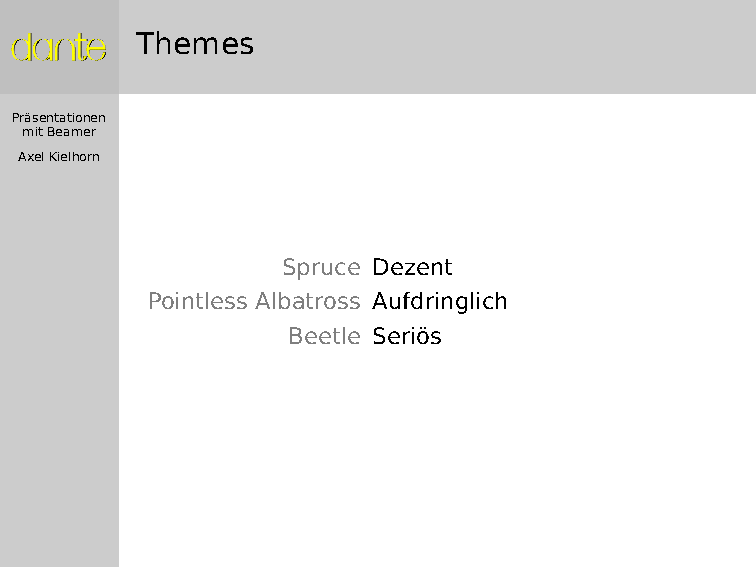
\includegraphics[width=\textwidth]{beamer-aufz2}
  \caption{Mit wenig Aufwand repariert.}
  \label{fig:aufz2}
\end{figure}

Auffälliger als Aufzählungen sind Blöcke. Beamer stellt drei Versionen zur
Verfügung, neben dem normalen \texttt{block} gibt es den \texttt{alertblock}
in rot und den \texttt{exampleblock} in grün. Da die Farben in einem grauen 
Farbtheme nicht erkennbar sind, wurde für Abbildung~\ref{fig:block} die 
Schrift verändert.

\begin{lfgwcode}{}
\setbeamerfont{block title example}{shape=\itshape}
\setbeamerfont{block body example}{family=\ttfamily}
\end{lfgwcode}

\begin{lfgwcode}{}
\begin{block}{Erstens}
    Nicht vergessen!
\end{block}
\begin{alertblock}{Zweitens}
    Unbedingt dran denken!
\end{alertblock}
\begin{exampleblock}{Drittens}
    Sehr wichtig!
\end{exampleblock}
\end{lfgwcode}

\begin{figure}
  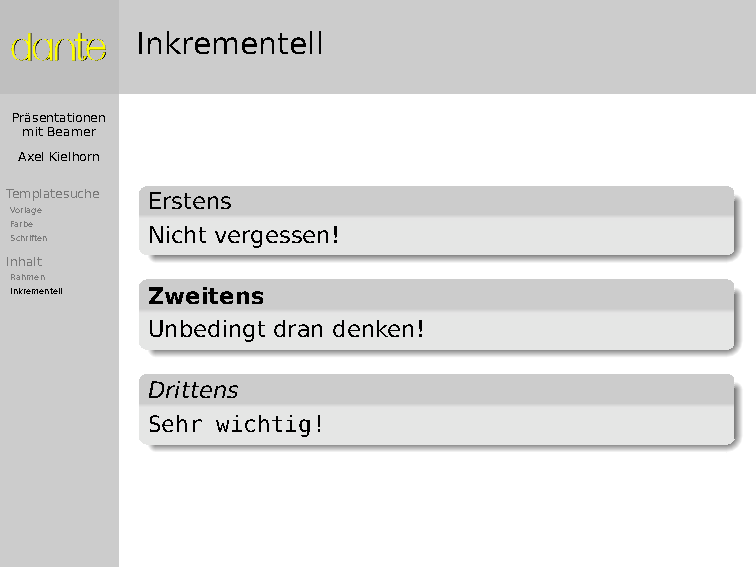
\includegraphics[width=\textwidth]{beamer-block}
  \caption{Blöcke statt Aufzählungen}
  \label{fig:block}
\end{figure}

\subsection{Inkrementelle Tabellen}

Bei Tabellen ist der Aufwand deutlich größer, es muss jedem Objekt
mitgeteilt werden, wann es sichtbar sein soll. Dies geschieht mit dem
\cs{uncover}-Befehl. Die Overlayspezifikationen \texttt{<2>} gibt an, das das
Objekt nur auf Seite 2 sichtbar ist. 

\begin{lfgwcode}{}
\begin{tabular}{llrrr}
Version    & Wert 1 & Wert 2          & \uncover<2>{Wert 2} \\
           &        &                 & \uncover<2>{optimiert}\\
2.7        & $0.85$ &           39\%  & \uncover<2>{35\%}\\
2.8        & $0.95$ & \alert<2>{49\%} & \uncover<2>{\alert<2>{44\%}}\\
2.9        & $0.98$ &           55\%  & \uncover<2>{51\%}
\end{tabular}
\end{lfgwcode}

Mehrere Objekte lassen sich in der \texttt{columns} Umgebung nebeneinander
platzieren. Die Spalten können oben \texttt{[t]}, unten \texttt{[b]} oder
zentriert \texttt{[c]} ausgerichtet werden.

Diese Art des Mehrspaltensatzes funktioniert nicht im
\textit{Article} Modus.

\begin{lfgwcode}{}
\begin{columns}[t]
  \begin{column}<1->{0.5\textwidth}
    Es ist so eng hier. Muss man das denn unbedingt zweispaltig setzen?
  \end{column}%
  \begin{column}<2->{0.5\textwidth}
    Ich will raus!
  \end{column}
\end{columns}
\end{lfgwcode}
  
\subsection{Übergänge}

Beamer unterstützt animierte Seitenwechsel, jedoch nur bei Verwendung von
Acrobat Reader, Evince oder Okular im Vollbildmodus. Die Befehle müssen auf
der Zielseite gegeben werden und gelten beim blättern auf diese Seite. Werden
sie für einen Frame gegeben, gelten sie für alle Seiten des Frames.

\begin{labeling}{\texttt{transblindshorizontal}}
  \item[\texttt{transdissolve}] Eine Seite löst sich in Punkten auf und eine neue entsteht
  \item[\texttt{transblindshorizontal}] oder \texttt{vertical}, der Jalousie-Effekt.
  \item[\texttt{transboxin}] oder \texttt{boxout}, rein- oder rauszoomen.
  \item[\texttt{transwipe}] Neue Seite wischt alte Seite weg.
\end{labeling}

\subsection{Sprünge}

Frames mit einem \texttt{label} können als Sprungziele verwendet werden.
Außerdem ist es möglich explizite Sprungziele zu definieren. Über einen
Hyperlink können diese Ziele angesprungen werden. Bei den Buttons handelt es
sich nur um Bilder, der \cs{beamerreturnbutton} bietet keine
Zurück-Funktion im Sinne eines Sprung-Stacks.

\begin{lfgwcode}{}
\hypertarget{Bilder}{}
\hyperlink{Bilder}{\beamergotobutton{Zu Bilder springen}}
\hyperlink{Bilder}{\beamerskipbutton{Zu Bilder springen}}
\hyperlink{Bilder}{\beamerreturnbutton{Zurück zu Bilder}}
\end{lfgwcode}

\begin{figure}
  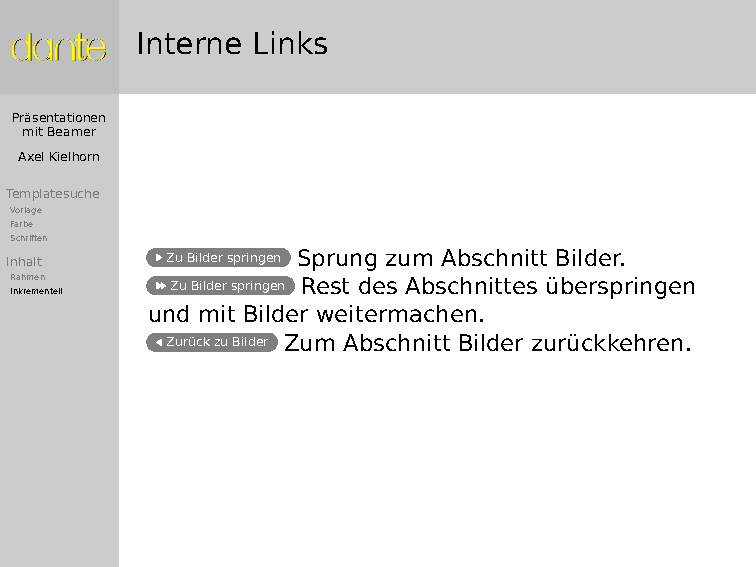
\includegraphics[width=\textwidth]{beamer-sprung}
  \caption{Sprünge zur näheren Erläuterung, oder bei Zeitmangel.}
  \label{fig:sprung}
\end{figure}

Die Überschriften im linken Rand sind ebenfalls Links.
Hier kann man schnell zum gewünschten Abschnitt springen.

\subsection{Bilder}

Bilder lassen sich wie gewohnt mit \cs{includegraphics} einbinden.

\begin{lfgwcode}{}
\includegraphics[width=\textwidth]{Bild.png}
\end{lfgwcode}

Benötigt man für ein großes Bild besonders viel Platz, kann man einen
\texttt{plain} Frame erzeugen. In diesem Fall ist die unterschiedliche
Skalierung für \textit{Beamer} und \textit{Article} zu beachten.

\begin{lfgwcode}{}
\begin{frame}[plain]
  \begin{centering}%
    \pgfimage<beamer>[width=1\paperwidth]{Bild.png}%
    \pgfimage<article>[width=1\textwidth]{Bild.png}%
    \par%
  \end{centering}%
\end{frame}
\end{lfgwcode}

Bei Themes mit farbigen Balken an der linken Seite funktioniert das nicht.
Hier muss für den \texttt{plain} Rahmen etwas mehr Aufwand getrieben werden.
Außerdem sind zwei \TeX-Läufe erforderlich.

\begin{lfgwcode}{}
\begin{frame}<beamer>[plain]
   \begin{tikzpicture}[remember picture,overlay]
      \node[at=(current page.center)] {\pgfimage[width=1\paperwidth]
      {Bild.png}};
   \end{tikzpicture}
\end{frame}
\end{lfgwcode}

\subsection{Tikz im Beamer}

Overlayspezifikationen funktionieren nicht nur für Text.
Im folgenden Beispiel wird im ersten Durchlauf das Koordinatenkreuz
gezeichnet und auf der zweiten Seite die Funktion geplottet.

Damit die zweite Seite nicht durchscheint und das Ergebnis verrät wird der
Uncovermodus explizit auf \texttt{invisible} gesetzt.

\begin{lfgwcode}{}
\mode<presentation>{
  \setbeamercovered{invisible}
}

\begin{frame}[fragile,label=tikz]{Tikz}
  \begin{tikzpicture}[scale=0.6]
     \draw[help lines] (0,0) grid (13,4);
     \draw[gray] (-0.4,0) node {0} (-0.4,1) node {1} 
                 (-0.4,2) node {2} (-0.4,3) node {3} (-0.4,4) node {4};
     \draw[gray] (0,-.4)  node {0} (3,-.4)  node {3} 
                 (6,-.4)  node {6} (9,-.4)  node {9} (12,-.4) node {12};
      \pgfplothandlerlineto 
      \onslide<2>\pgfplotxyfile{Daten.dat}
      \pgfusepath{stroke}
  \end{tikzpicture}
\end{frame}
\end{lfgwcode}

\subsection{Hintergrundbilder}

Natürlich kann man den Standardhintergrund durch ein Bild ersätzen, entweder
für die gesamte Präsentation, oder für einzelne Frames. Auch hier ist es
erforderlich den Präsentationsmodus zu aktivieren, um das
\texttt{backgroundtemplate} zu definieren.

\begin{lfgwcode}{}
\mode<presentation>{
\usebackgroundtemplate{\includegraphics[width=\paperwidth]{Hintergrund}}
}

\begin{frame}<beamer>[plain,b] % b = bottom
  \huge\bfseries\color{structure!15} Noch Fragen?
  \vspace{0.3cm} % Etwas Luft nach unten
\end{frame}

\mode<presentation>{
\usebackgroundtemplate{}
}
\end{lfgwcode}

Und damit schließt die Präsentation.

\begin{lfgwcode}{}
\end{document}
\end{lfgwcode}

Die komplette Anleitung (\cite{tantau:beamer}) zu \paket{Beamer} ist Bestandteil von \TeXLive{} und kann
über den Befehl \texttt{texdoc beamer} aufgerufen werden.

Außerdem gibt es noch ein Buch von Herbert Voß aus der Dante-Edition: \cite{voss:praesentationen}



% !TeX root = lfgw.tex
\chapter{Eigene \LaTeX-Erfindungen dokumentieren}%%%MS: Erfindungen finde ich den falschen Begriff

Man muss kein besonders gewiefter \TeX{}niker sein, um in die Verlegenheit zu kommen, eigene 
\LaTeX-\enquote{Erfindungen} dokumentieren zu müssen
-- und sei es nur ein einzelnes kleines \lstinline/\renewcommand/
im Rahmen eines Projektes mit mehreren Mitarbeitern.

Auf den zweiten Blick ist dies für Geisteswissenschaftler gar nicht so anders, 
als die anderen Dinge auch, die Philologen mit Textverarbeitungsprogrammen so anstellen:

dokumentierter text  ---  dokumentierender text ...


\minisec{Wiedergabe der \TeX-typischen Logos}

Das Paket \paket{hologo} von Heiko Oberdiek stellt den Befehl \lstinline/\hologo{Name}/ zur 
Verfügung, das u.\,a. folgende Logos erzeugen kann:

\begin{center}
 \begin{tabular}{ll}
  (La)TeX & \hologo{(La)TeX} \\
  AmSLaTeX & \hologo{AmSLaTeX} \\
  AmSTeX & \hologo{AmSTeX} \\
  biber & \hologo{biber} \\
  BibTeX & \hologo{BibTeX} \\
  HanTheThanh & \hologo{HanTheThanh} \\
  KOMAScript & \hologo{KOMAScript} \\
  La & \hologo{La} \\
  LaTeX & \hologo{LaTeX} \\
  LaTeX2e & \hologo{LaTeX2e} \\
  LaTeX3 & \hologo{LaTeX3} \\
  LaTeXe & \hologo{LaTeXe} \\
  LuaLaTeX & \hologo{LuaLaTeX} \\
  LuaTeX & \hologo{LuaTeX} \\
  LyX & \hologo{LyX} \\
  METAFONT & \hologo{METAFONT} \\
  MetaFun & \hologo{MetaFun} \\
  METAPOST & \hologo{METAPOST} \\
  MetaPost & \hologo{MetaPost} \\
  MiKTeX & \hologo{MiKTeX} \\
  teTeX & \hologo{teTeX} \\
  TeX & \hologo{TeX} \\
  Xe & \hologo{Xe} \\
  XeLaTeX & \hologo{XeLaTeX} \\
  XeTeX & \hologo{XeTeX} \\
 \end{tabular}

\end{center}





\minisec{Listings einbinden}

\paket{listings}


\minisec{Latex-Quelltext und seine Ausgabe wiedergeben}

\paket{showexpl}

% !TeX root = lfgw.tex
\chapter{Anhang}

\section{Ein Beispiel, das (fast) alles kann}

In der folgenden Musterdatei wird (fast) alles vorgeführt, was das Skript erklärt.
Sie kompiliert in kile durch ALT+6...

\lstinputlisting{lfgw-musterdatei}


\section{Unicode}
\label{unicode} \index{Unicode}

\subsection{Einstellen des Editors auf Unicode}

\subsection{Umcodieren vorhandener Dateien}

Programm recode


\subsection{Häufig benötigte Unicode-Zeichen}

\label{utf8codes}

\section{Wie installiere ich die Software/Pakete etc.}

\minisec{Die radikale Alternative: Cloud-Lösung}
\index{overleaf}
\index{sharelatex}


\minisec{Windows: miktex}
\index{miktex}

\minisec{Standardwerkzeug der Linux-Distribution}

\minisec{ctan}
\index{ctan}


\section{Woher beziehe ich Dokumentation zu den Paketen?}

\minisec{Welche Pakete könnten interessant sein?}

ctan

\minisec{Wie funktionieren die schon installierten Pakete?}

texdoc PAKETNAME


\section{Welche Bücher sollte ich mir kaufen?}

Erster Schritt: Dokument \enquote{\LaTeXe -Kurzbeschreibung} mit 
\lstinline/texdoc lshort/. Dieses Dokument (ca. 50 Seiten) sollte man am besten ausdrucken.

Einen grundlegenden Überblick über das Gesamtsystem bietet
\cite{voss:einfuehrung}

Wenn man sich zur Benutzung der \KOMAScript -Klassen entscheidet, ist die ultimative Referenz,
mit der man erst das ganze Paket ausnutzen kann:
\cite{kohm:2014}

Die einzige Spezialmonographie zum Thema \LaTeX{} in den Geisteswissenschaften ist
\cite{rouquette:2012}

Ideal zum Nachschlagen bestimmter Befehle eignet sich:
\cite{voss:referenz}

Spezialtitel, je nach individuellem Bedürfnis:

\cite{voss:praesentationen}

\cite{voss:bibliografien}

\cite{voss:pstricks}


\section{Bücher veralten. Wer hält mich auf dem Laufenden?}

dante e.\,V.

\printbibliography
\chapter{Register} %%%MS: Besser \addchap
\printindex          % der "allgemeine" Index
\printindex[pakete]


\vfill
\minisec{Kolophon}

opensuse 13.2 auf lenovo ideapad s10e von 2008

kile

pdflatex mit \KOMAScript 

Klasse scrbook

geometry, DIV,  BCOR ...

babel

lstlisting

biblatex und biber

Bibliografiestil der Historischen Zeitschrift (\lstinline/\usepackage[style=historische-zeitschrift]{biblatex}/)

imakeidx
\end{document}
